% !TeX program = pdflatex
% !TeX root = main.tex
\documentclass[12pt, a4paper, oneside]{article}
\usepackage[utf8]{inputenc}
\usepackage[T5]{fontenc}
\usepackage[vietnamese]{babel}
\usepackage[top = 2.5cm, bottom = 2.5cm, left = 1.5cm, right = 1cm]{geometry}
\usepackage{amsmath,amsfonts,amssymb}
\usepackage{indentfirst,enumitem}
\usepackage{graphicx}
\usepackage{multicol}
\usepackage{multirow}
\usepackage{setspace}
\usepackage{hyperref}
\usepackage{listings}
\usepackage{tabularx}
\usepackage{hyperref}
\usepackage{xcolor}
\usepackage{scrextend}
\usepackage{comment}

\usepackage{tipa}
\usepackage{subcaption}
\usepackage{caption}
\usepackage{booktabs}
\usepackage{array}
\usepackage{fancyhdr}
\usepackage{algorithm2e}
\usepackage{float}
\usepackage[most]{tcolorbox}
\usepackage{pdfpages}
\usepackage{import}
\graphicspath{ {figures/} }
\usepackage{titlesec}
\usepackage{listingsutf8}

\lstset{
    inputencoding=utf8,
    extendedchars=true,
    literate=
        {á}{{\'a}}1 {à}{{\`a}}1 {ả}{{\?a}}1 {ã}{{\~a}}1 {ạ}{{\.a}}1
}

\titleformat{\paragraph}
{\normalfont\normalsize\bfseries}
{\theparagraph}{1em}{}

\titlespacing*{\paragraph}
{0pt}{3ex plus 1ex minus .2ex}{1em}
\usepackage{float}
\usepackage{tikz}
\usetikzlibrary{calc, positioning, shapes.geometric}
\usetikzlibrary{circuits.logic.US, circuits.logic.IEC}

\captionsetup[figure]{labelfont=bf, textfont=it, font=small}

\hypersetup{
    colorlinks=true,
    linkcolor=black,
    filecolor=magenta,      
    urlcolor=black,
    pdftitle={TKHTN},
    pdfpagemode=FullScreen,
}

%\changefontsizes{13pt}
\renewcommand\thesection{\arabic{section}.}
\renewcommand\thesubsection{\arabic{section}.\arabic{subsection}}

\pagestyle{fancy}
\fancypagestyle{plain}{\fancyhf{}}
\fancyhead[r]{\textit{Bộ môn Điện tử}}
%\fancyhead[c]{\bfseries DSP}
\fancyhead[l]{\textit{Thiết kế vi mạch}}
\renewcommand{\headrulewidth}{0.2pt}
\setlength{\headheight}{10pt}


\def\mathrlap{\mathpalette\mathrlapinternal} 
\def\mathclap{\mathpalette\mathclapinternal}
\def\mathllapinternal#1#2{\llap{$\mathsurround=0pt#1{#2}$}}
\def\mathrlapinternal#1#2{\rlap{$\mathsurround=0pt#1{#2}$}}

%CHÈN ẢNH
\usepackage{pgfplots}
\pgfplotsset{compat=1.15}
\usepackage{mathrsfs}
\usetikzlibrary{arrows}
\usetikzlibrary[patterns]

%New colors defined below
\definecolor{codegreen}{rgb}{0,0.6,0}
\definecolor{codegray}{rgb}{0.5,0.5,0.5}
\definecolor{codepurple}{rgb}{0.58,0,0.82}
\definecolor{backcolour}{rgb}{0.95,0.95,0.92}

\input{verilogstyle}
\setlength{\headheight}{14.94pt}
\begin{document}
\thispagestyle{empty}
% Định nghĩa macro vẽ ký hiệu tam giác cho chân Clock
\def\clktriangle#1#2{
    \draw (#1, #2) ++(0, 0.15) -- ++(0.2, -0.15) -- ++(-0.2, -0.15);
}
\begin{titlepage}
%\SetWatermarkText{\includegraphics[width = 0.97\paperwidth,
%height = 0.97\paperheight]{bia.png}}
%\SetWatermarkAngle{0} 
%\SetWatermarkText{\includegraphics[scale=1]{hust.png}}
%\SetWatermarkAngle{0} 
\begin{tikzpicture}[remember picture,overlay,inner sep=0,outer sep=0]
     \draw[blue!70!black,line width=4pt] ([xshift=-1.5cm,yshift=-2cm]current page.north east) coordinate (A)--([xshift=1.5cm,yshift=-2cm]current page.north west) coordinate(B)--([xshift=1.5cm,yshift=2cm]current page.south west) coordinate (C)--([xshift=-1.5cm,yshift=2cm]current page.south east) coordinate(D)--cycle;

     \draw ([yshift=0.5cm,xshift=-0.5cm]A)-- ([yshift=0.5cm,xshift=0.5cm]B)--
     ([yshift=-0.5cm,xshift=0.5cm]B) --([yshift=-0.5cm,xshift=-0.5cm]B)--([yshift=0.5cm,xshift=-0.5cm]C)--([yshift=0.5cm,xshift=0.5cm]C)--([yshift=-0.5cm,xshift=0.5cm]C)-- ([yshift=-0.5cm,xshift=-0.5cm]D)--([yshift=0.5cm,xshift=-0.5cm]D)--([yshift=0.5cm,xshift=0.5cm]D)--([yshift=-0.5cm,xshift=0.5cm]A)--([yshift=-0.5cm,xshift=-0.5cm]A)--([yshift=0.5cm,xshift=-0.5cm]A);


     \draw ([yshift=-0.3cm,xshift=0.3cm]A)-- ([yshift=-0.3cm,xshift=-0.3cm]B)--
     ([yshift=0.3cm,xshift=-0.3cm]B) --([yshift=0.3cm,xshift=0.3cm]B)--([yshift=-0.3cm,xshift=0.3cm]C)--([yshift=-0.3cm,xshift=-0.3cm]C)--([yshift=0.3cm,xshift=-0.3cm]C)-- ([yshift=0.3cm,xshift=0.3cm]D)--([yshift=-0.3cm,xshift=0.3cm]D)--([yshift=-0.3cm,xshift=-0.3cm]D)--([yshift=0.3cm,xshift=-0.3cm]A)--([yshift=0.3cm,xshift=0.3cm]A)--([yshift=-0.3cm,xshift=0.3cm]A);

   \end{tikzpicture}
\begin{center}
    \vspace{7pt}
        \textbf{ĐẠI HỌC QUỐC GIA THÀNH PHỐ HỒ CHÍ MINH}
    
    \vspace{7pt}
    \textbf{TRƯỜNG ĐẠI HỌC BÁCH KHOA}
    
    \vspace{7pt}
    \textbf{KHOA ĐIỆN - ĐIỆN TỬ}
\end{center}
\vspace{10pt}
\begin{center}
    
\includegraphics[scale=0.3]{HCMUT.png}
    \vspace{10pt}
\end{center}

\begin{center}
    \fontsize{18pt}{17pt}\selectfont 
    \textbf{BÁO CÁO THÍ NGHIỆM}

    \textbf{MÔN:  THIẾT KẾ VI MẠCH}
\end{center}
\begin{center}
    \fontsize{15pt}{17pt}\selectfont 
    \textbf{\textrm{LAB 2: Synthesis and Standard Cell}}
\end{center}

\begin{center}
    \vspace{15pt}
    \textbf{Lớp: L03 - NHÓM: 5}
    
    \textbf{GVHD: ThS. Nguyễn Trung Hiếu}
\end{center}

\vspace{10pt}

\begin{table}[h!]
\centering
\begin{tabular}{|c|c|c|}
\hline
\textbf{MSSV} & \textbf{Họ và tên} & \textbf{Tỉ lệ phân công} \\ \hline
2311267 & Vũ Nhật Huy & 100\% \\ \hline
2313355 & Nguyễn Minh Thuận & 100\% \\ \hline
2313222 & Thái Đức Thiên & 100\% \\ \hline
\end{tabular}
\end{table}
\vfill
\centerline{\bf Thành phố Hồ Chí Minh, tháng 4 năm 2026}

\vspace{1cm}
\end{titlepage}
\newpage
\tableofcontents
\newpage
\section{Experiment 1}
\subsection{Code và testbench}
\subsubsection{NOT}
\begin{lstlisting}[style={prettyverilog}, caption={\texttt{code thiết kế cổng NOT}}]
`timescale 1ns/1ps
module not(
    input logic A,
	  output logic Y);
    assign Y = ~A;
endmodule
\end{lstlisting}
\begin{lstlisting}[style={prettyverilog}, caption={\texttt{code testbench cổng NOT}}]
`timescale 1ns/1ps
module tb_not;
    logic A;
    logic Y;
    not(.A(A), .Y(Y));
    inital begin
        $dumpfile("not_wave.vcd");
        $dumpvars(0, tb_not);
        A = 0; #10;
        A = 0; #10;
        A = 1; #10;
        A = 1; #10;
        $finish;
    end
endmodule
\end{lstlisting}

Trước hết, nhóm thực hiện kiểm chứng chức năng logic và đo đạc độ trễ truyền dẫn cơ bản của cổng NOT. Hình \ref{fig:exp1_not_func} thể hiện dạng sóng ngõ vào và ngõ ra, qua đó xác nhận đặc tính đảo pha của linh kiện.

\begin{figure}[H]
    \centering
    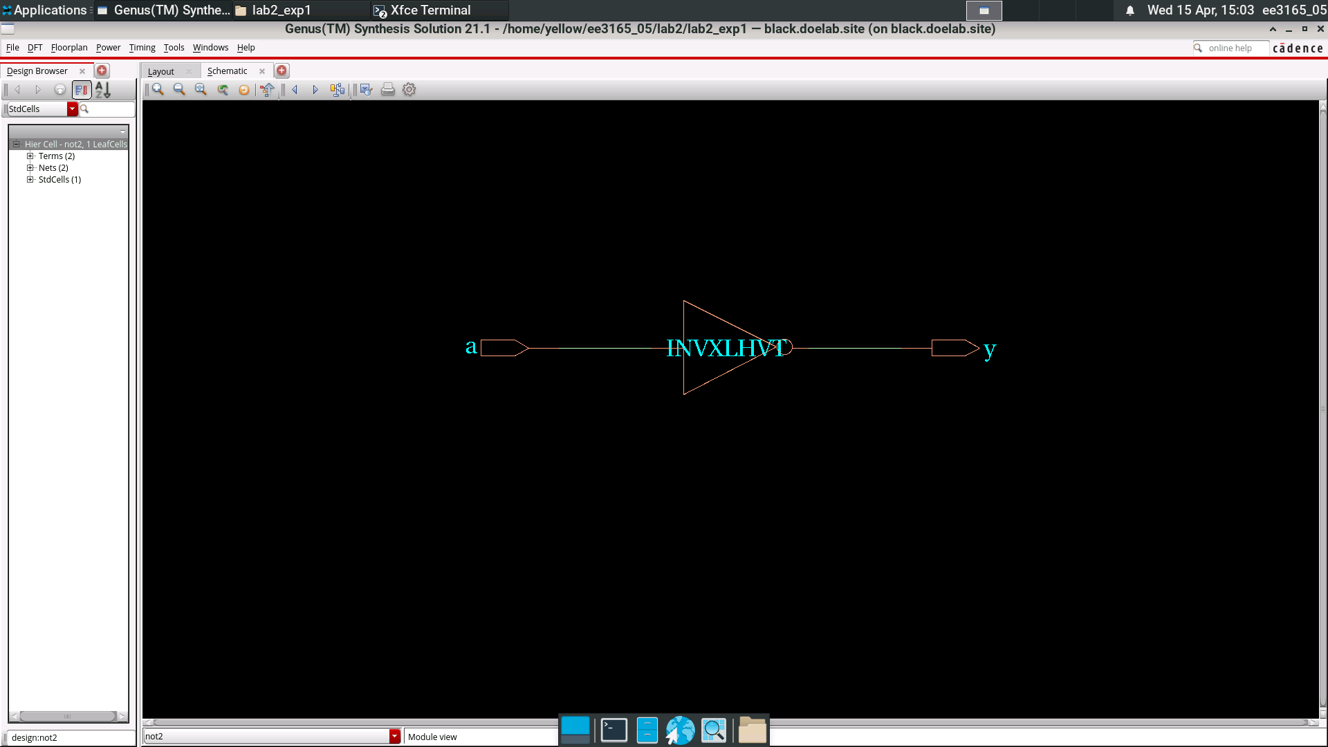
\includegraphics[width=0.9\textwidth]{figures/exp1_not.png}
    \caption{Waveform kiểm chứng chức năng và đo độ trễ truyền dẫn cổng NOT. Đường màu xanh là tín hiệu ngõ vào A, đường màu đỏ là đáp ứng ngõ ra Y.}
    \label{fig:exp1_not_func}
\end{figure}

Nhóm thực hiện khảo sát đặc tính của cổng NOT trên cả hai loại thư viện: High Threshold Voltage (HVT) và Low Threshold Voltage (LVT) để đánh giá sự đánh đổi giữa tốc độ và công suất.

\paragraph{A. Thư viện High Threshold Voltage (HVT)}
Đặc tính của các cell HVT là dòng rò thấp nhưng độ trễ lớn hơn. Kết quả mô phỏng 8 corners được tổng hợp trong bảng dưới đây:

\begin{table}[H]
\centering
\renewcommand{\arraystretch}{1.3}
\resizebox{\textwidth}{!}{
\begin{tabular}{|l|c|c|c|c|}
\hline
\multirow{2}{*}{\textbf{Library Name}} 
& \multirow{2}{*}{\textbf{Total Area}} 
& \multirow{2}{*}{\textbf{Total Power}} 
& \multicolumn{2}{c|}{\textbf{Delay Parameter}} \\
\cline{4-5}

& & 
& \textbf{Rising Delay (ns)} 
& \textbf{Falling Delay (ns)} \\
\hline

% ----------- KHỐI HVT ----------------
fast\_vdd1v0\_basicCells\_hvt & 0.684 & 5.9274e-09 & 0.004 & 0.004 \\ \hline
fast\_vdd1v2\_basicCells\_hvt & 0.684 & 8.6130e-09 & 0.003 & 0.003 \\ \hline
slow\_vdd1v0\_basicCells\_hvt & 0.684 & 3.9947e-09 & 0.009 & 0.015 \\ \hline
slow\_vdd1v2\_basicCells\_hvt & 0.684 & 5.8211e-09 & 0.006 & 0.008 \\ \hline


\end{tabular}
}
\caption{Tổng hợp thông số Diện tích, Công suất và Độ trễ của cổng NOT qua 8 process corners.}
\label{tab:exp1_not_all_params}
\end{table}


Dưới đây là sự so sánh dạng sóng mô phỏng của cổng NOT tại hai góc cực đoan: Fast (nhanh nhất) và Slow (chậm nhất) ở cùng mức điện áp 1.0V.

\begin{figure}[H]
    \centering
    % --- Hình bên trái: Corner Fast ---
    \begin{subfigure}[b]{0.48\textwidth}
        \centering
        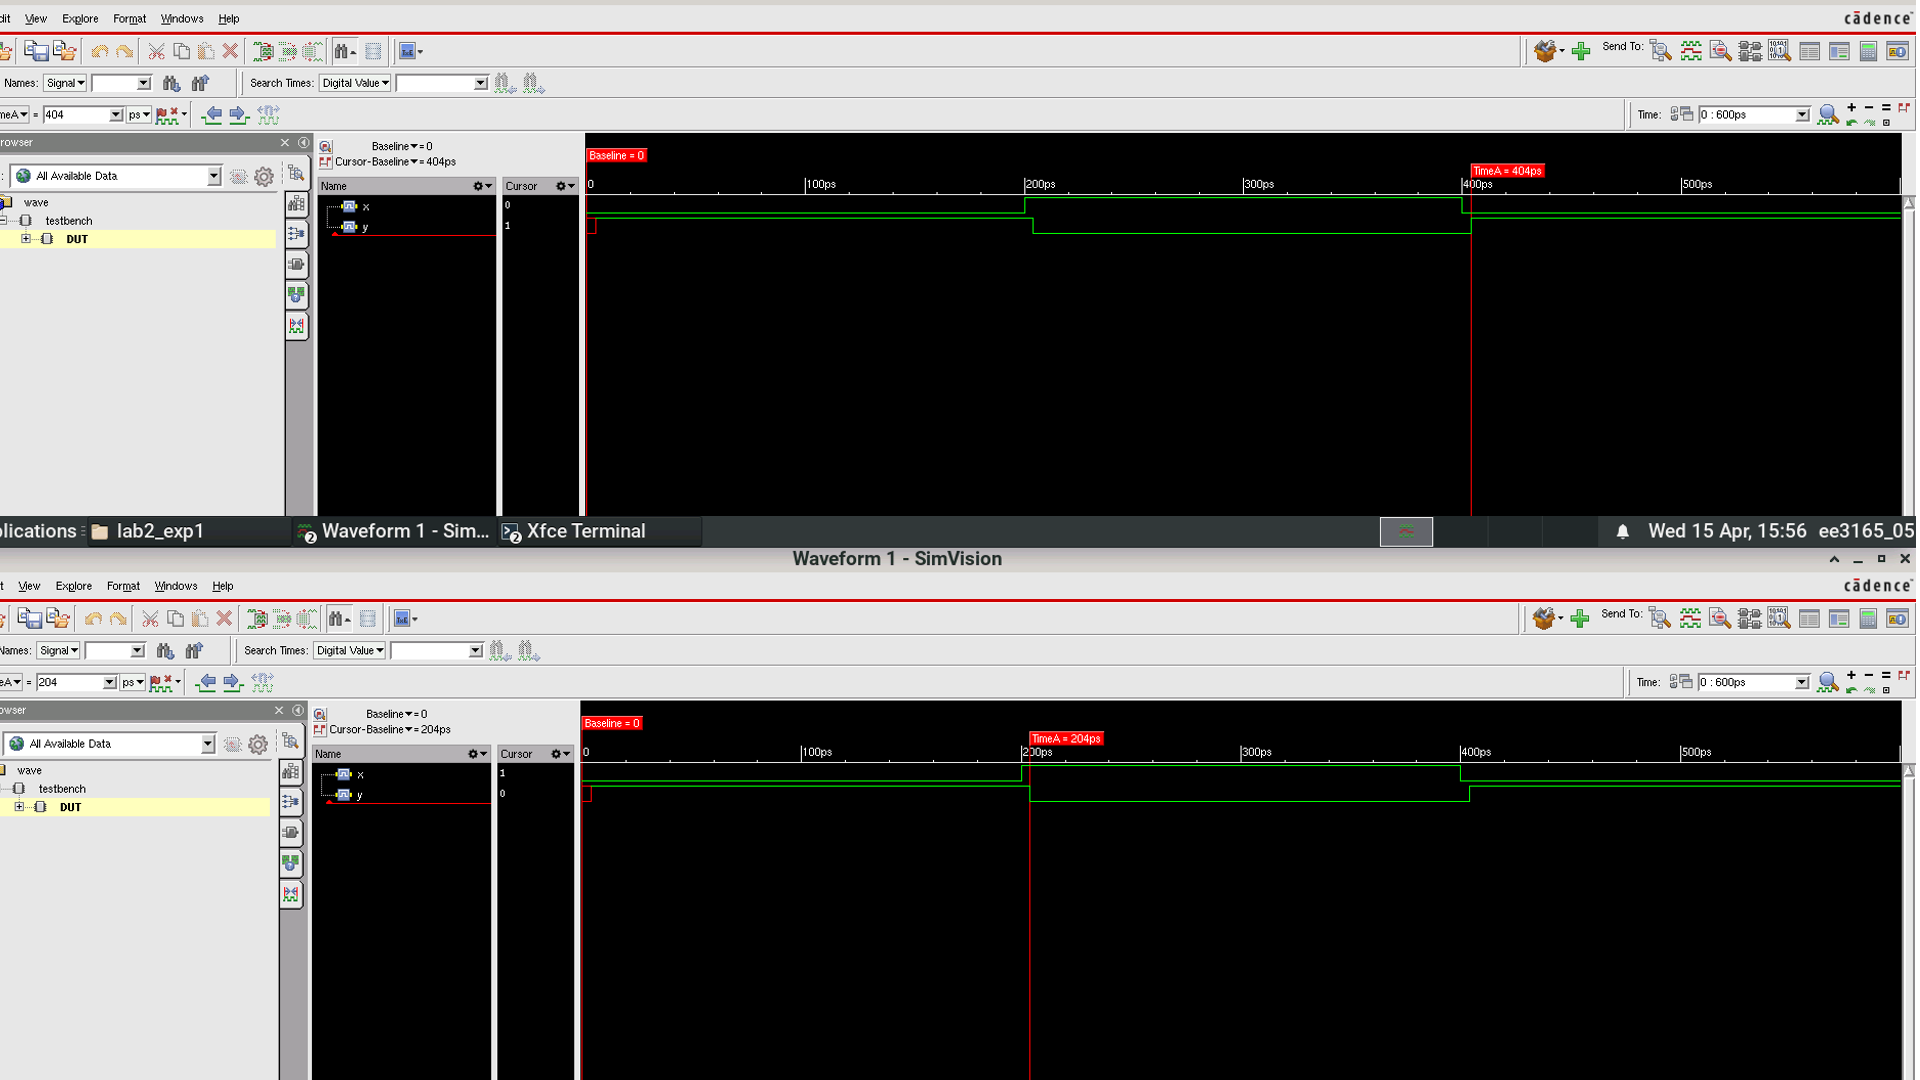
\includegraphics[width=\textwidth]{figures/exp1_not_fast_1v0.png}
        \caption{Corner HVT Fast (fast\_vdd1v0)}
        \label{fig:not_fast}
    \end{subfigure}
    \hfill
    % --- Hình bên phải: Corner Slow ---
    \begin{subfigure}[b]{0.48\textwidth}
        \centering
        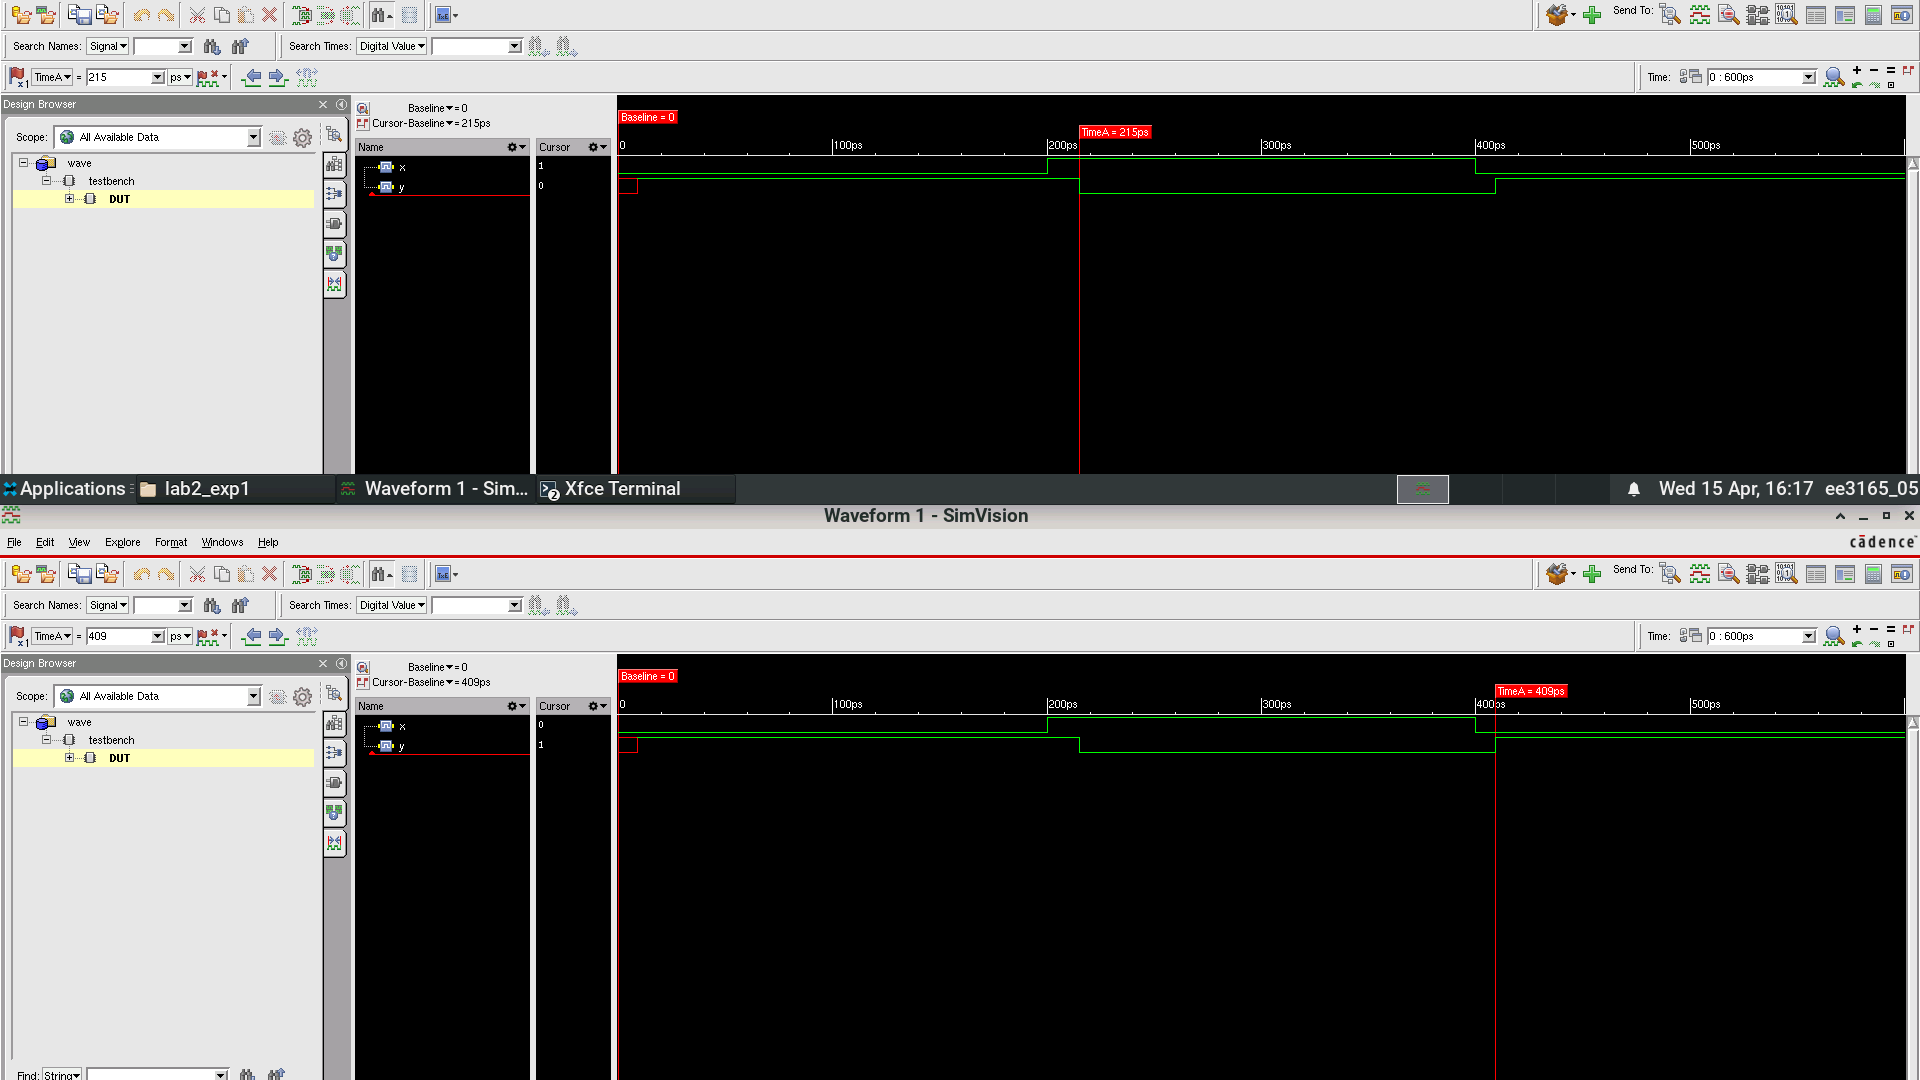
\includegraphics[width=\textwidth]{figures/exp1_not_slow_1v0.png}
        \caption{Corner HVT Slow (slow\_vdd1v0)}
        \label{fig:not_slow}
    \end{subfigure}
    
    \caption{So sánh Waveform đo độ trễ cổng NOT ở High Threshold Voltage. Lưu ý sự khác biệt về độ dốc của sườn tín hiệu và giá trị Delta T (độ trễ) giữa hai trường hợp.}
    \label{fig:not_comparison}
\end{figure}

\textbf{Nhận xét:} Đối với thư viện High Threshold Voltage (HVT), khi điện áp cung cấp giảm từ 1.2V xuống 1.0V, ta quan sát thấy các hiện tượng sau:
\begin{itemize}
    \item \textbf{Hiện tượng đói dòng:} Do các cell HVT vốn có điện áp ngưỡng ($V_{th}$) cao, việc hạ $V_{DD}$ xuống 1.0V làm cho điện áp quá lái ($V_{OV} = V_{DD} - V_{th}$) bị thu hẹp đáng kể. Dòng điện bão hòa ($I_{on}$) bị suy giảm mạnh, khiến thời gian nạp/xả các tụ ký sinh kéo dài.
    \item \textbf{Suy giảm tốc độ nghiêm trọng:} Hậu quả của việc thiếu dòng là độ trễ ($t_{pd}$) tăng vọt. Đặc biệt tại góc cực đoan \texttt{slow\_vdd1v0\_hvt}, độ trễ sườn xuống đạt mức lớn nhất là $0.015ns$. Đây là góc worst-case bắt buộc kỹ sư phải kiểm tra timing cẩn thận để tránh vi phạm Setup Time.
    \item \textbf{Tối ưu hóa năng lượng:} Bù lại nhược điểm về tốc độ, các cell HVT ở 1.0V cho thấy khả năng tiết kiệm điện tuyệt vời. Tổng công suất tại góc \texttt{slow\_vdd1v0\_hvt} đạt mức thấp kỷ lục ($3.99 \times 10^{-9}$ W), vô cùng lý tưởng cho các khối mạch không yêu cầu tốc độ cao.
\end{itemize}

Dưới đây là kết quả mô phỏng dạng sóng của cổng NOT sử dụng thư viện High Threshold Voltage (HVT) tại điều kiện điện áp danh định 1.2V.

\begin{figure}[H]
    \centering
    % --- Hình bên trái: Corner Fast ---
    \begin{subfigure}[b]{0.48\textwidth}
        \centering
        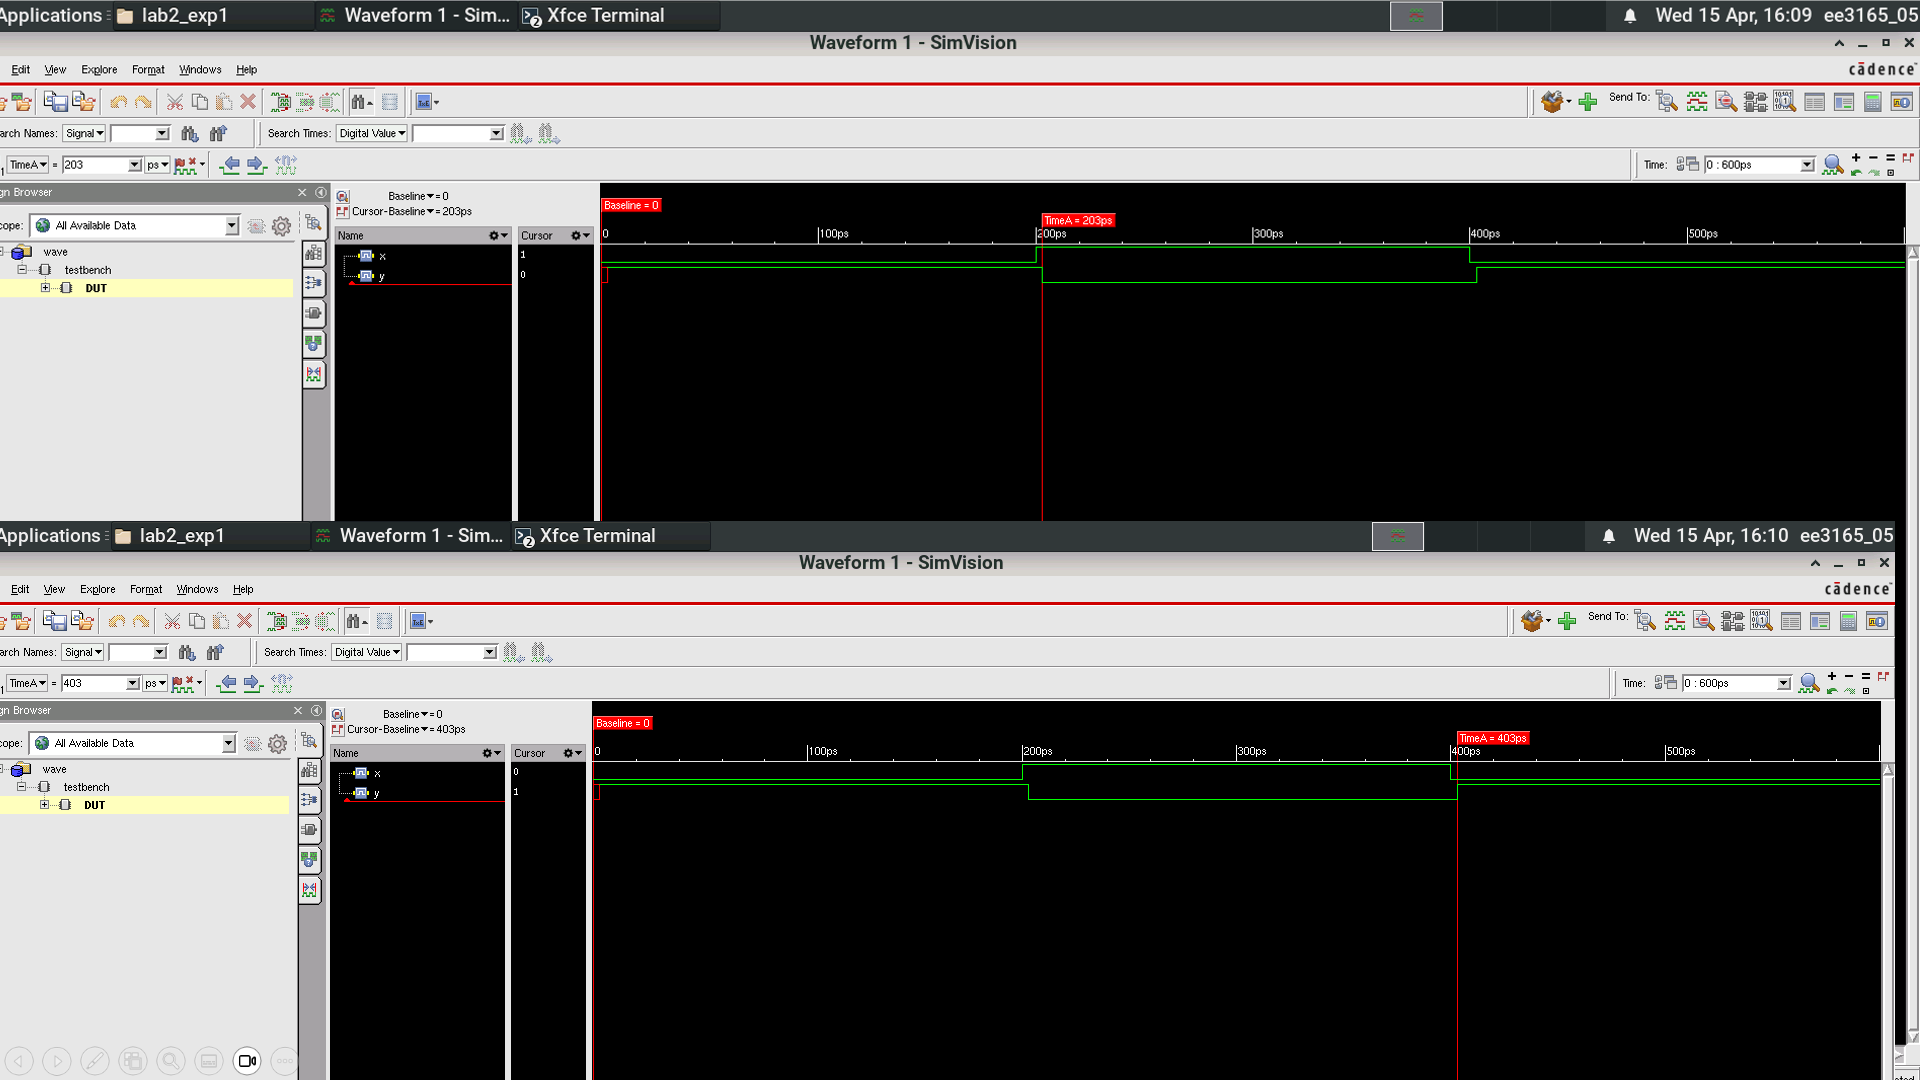
\includegraphics[width=\textwidth]{figures/exp1_hvt_not_fast_1v2.png}
        \caption{Corner HVT Fast (fast\_vdd1v2)}
        \label{fig:not_fast}
    \end{subfigure}
    \hfill
    % --- Hình bên phải: Corner Slow ---
    \begin{subfigure}[b]{0.48\textwidth}
        \centering
        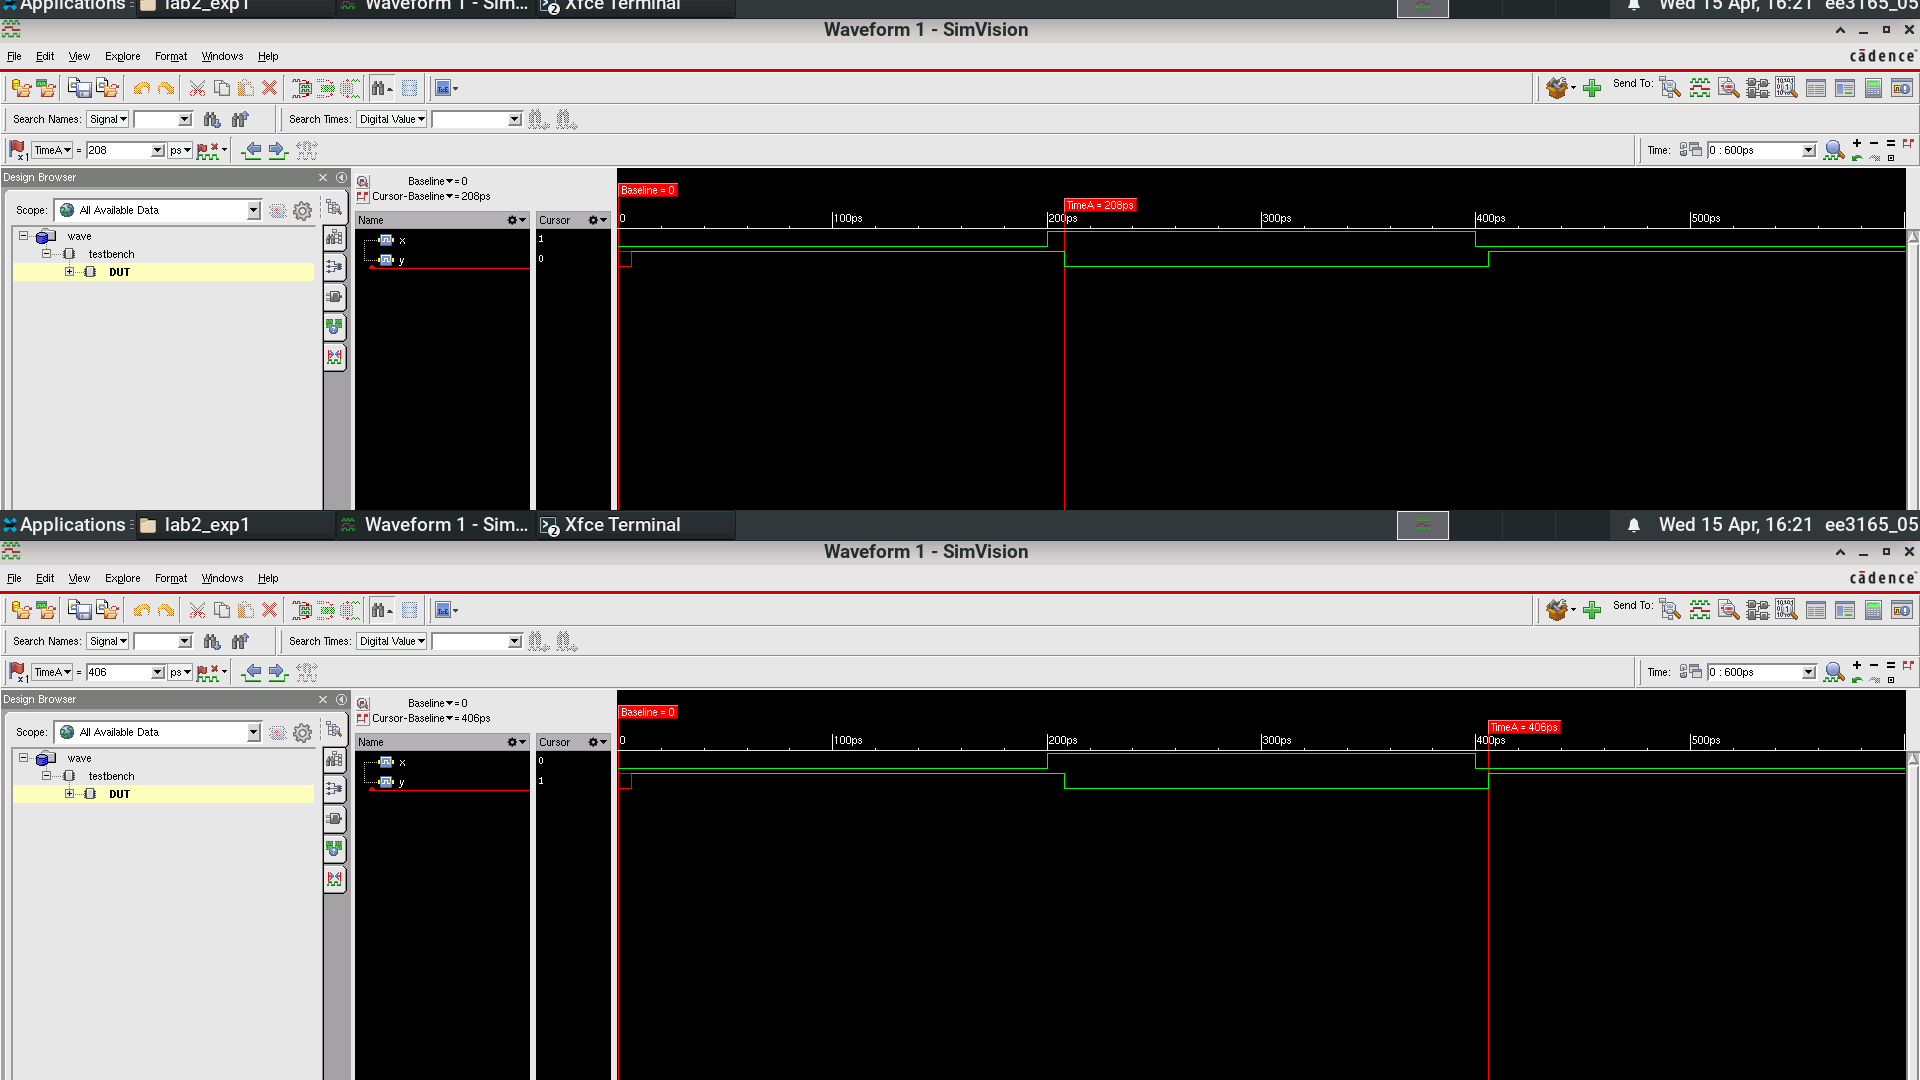
\includegraphics[width=\textwidth]{figures/exp1_hvt_not_slow_1v2.png}
        \caption{Corner HVT Slow (slow\_vdd1v2)}
        \label{fig:not_slow}
    \end{subfigure}
    \caption{So sánh Waveform đo độ trễ cổng NOT ở High Threshold Voltage với VDD = 1.2V}
    \label{fig:not_comparison}
\end{figure}

\textbf{Nhận xét:} Khi nâng điện áp cung cấp lên 1.2V cho thư viện High Threshold Voltage:
\begin{itemize}
    \item \textbf{Cải thiện tốc độ đáng kể:} Điện áp quá lái ($V_{GS} - V_{th}$) tăng lên giúp dòng điện $I_{on}$ mạnh hơn. So với mức 1.0V, độ trễ tại góc \texttt{fast\_vdd1v2\_hvt} giảm xuống chỉ còn $0.003ns$, là mức hiệu năng rất cao đối với dòng HVT.
    \item \textbf{Sự đánh đổi về công suất:} Công suất tiêu thụ tổng cộng tăng lên (khoảng $8.61 \times 10^{-9}$ W) do thành phần công suất động tỷ lệ thuận với bình phương điện áp nguồn ($P_{dyn} \propto V_{DD}^2$).
\end{itemize}

\paragraph{B. Thư viện Low Threshold Voltage (LVT)}

Ngược lại, các cell LVT cho tốc độ chuyển mạch nhanh hơn nhờ điện áp ngưỡng thấp, đổi lại công suất tiêu thụ tĩnh sẽ cao hơn đáng kể.

\begin{table}[H]
\centering
\renewcommand{\arraystretch}{1.3}
\resizebox{\textwidth}{!}{
\begin{tabular}{|l|c|c|c|c|}
\hline
\multirow{2}{*}{\textbf{Library Name}} 
& \multirow{2}{*}{\textbf{Total Area}} 
& \multirow{2}{*}{\textbf{Total Power}} 
& \multicolumn{2}{c|}{\textbf{Delay Parameter}} \\
\cline{4-5}

& & 
& \textbf{Rising Delay (ns)} 
& \textbf{Falling Delay (ns)} \\
\hline


% ----------- KHỐI LVT ----------------
fast\_vdd1v0\_basicCells\_lvt & 0.684 & 7.8029e-09 & 0.003 & 0.003 \\ \hline
fast\_vdd1v2\_basicCells\_lvt & 0.684 & 1.07250e-08 & 0.003 & 0.003 \\ \hline
slow\_vdd1v0\_basicCells\_lvt & 0.684 & 4.28894e-09 & 0.006 & 0.007 \\ \hline
slow\_vdd1v2\_basicCells\_lvt & 0.684 & 6.20997e-09 & 0.004 & 0.005 \\ \hline

\end{tabular}
}
\caption{Tổng hợp thông số Diện tích, Công suất và Độ trễ của NOT (Thư viện LVT).}
\label{tab:exp2_lvt_params_framed}
\end{table}

Sau khi khảo sát thư viện HVT, nhóm tiếp tục thực hiện mô phỏng với thư viện LVT để đánh giá sự cải thiện về tốc độ. Dưới đây là kết quả waveform tại hai corner Fast và Slow ở mức điện áp 1.0V.

\begin{figure}[H]
    \centering
    % --- Hình bên trái: LVT Fast ---
    \begin{subfigure}[b]{0.48\textwidth}
        \centering
        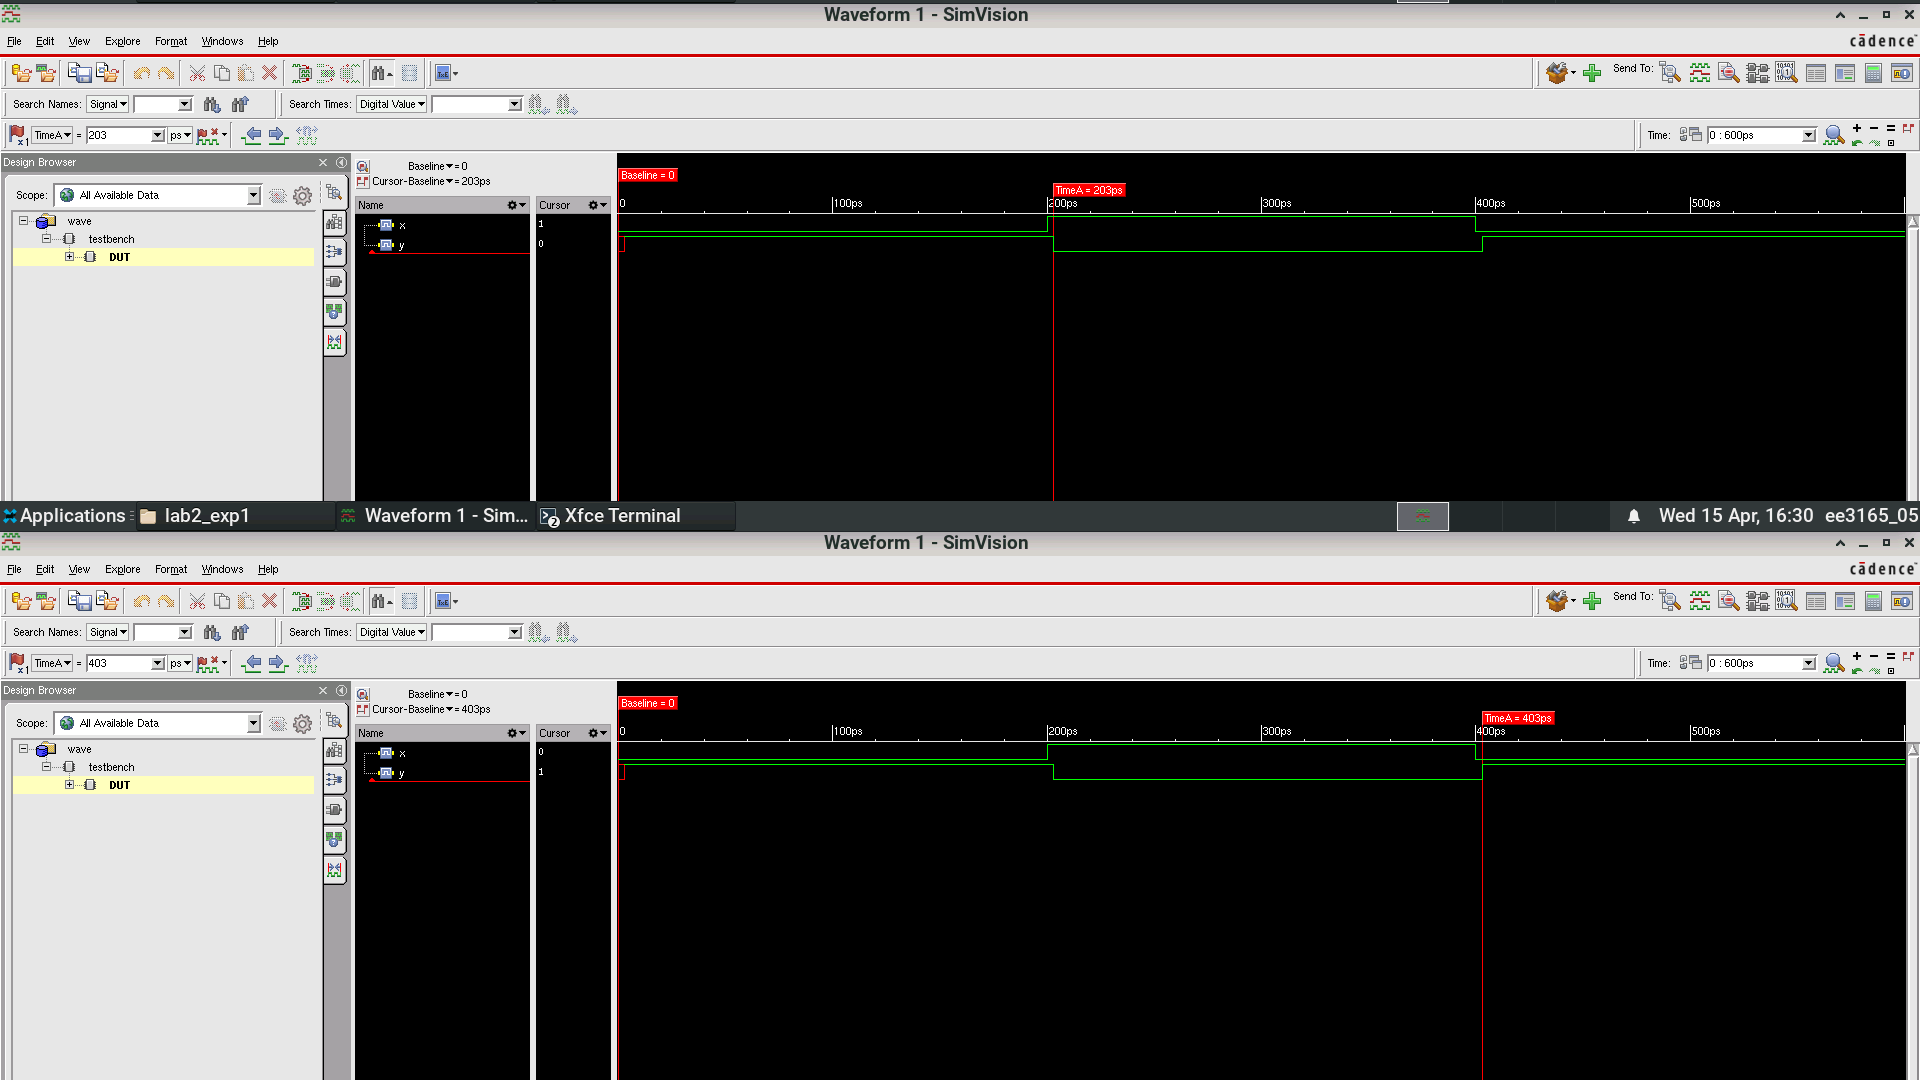
\includegraphics[width=\textwidth]{figures/exp1_lvt_not_fast_1v0.png}
        \caption{Corner LVT Fast (fast\_vdd1v0)}
        \label{fig:not_lvt_fast}
    \end{subfigure}
    \hfill
    % --- Hình bên phải: LVT Slow ---
    \begin{subfigure}[b]{0.48\textwidth}
        \centering
        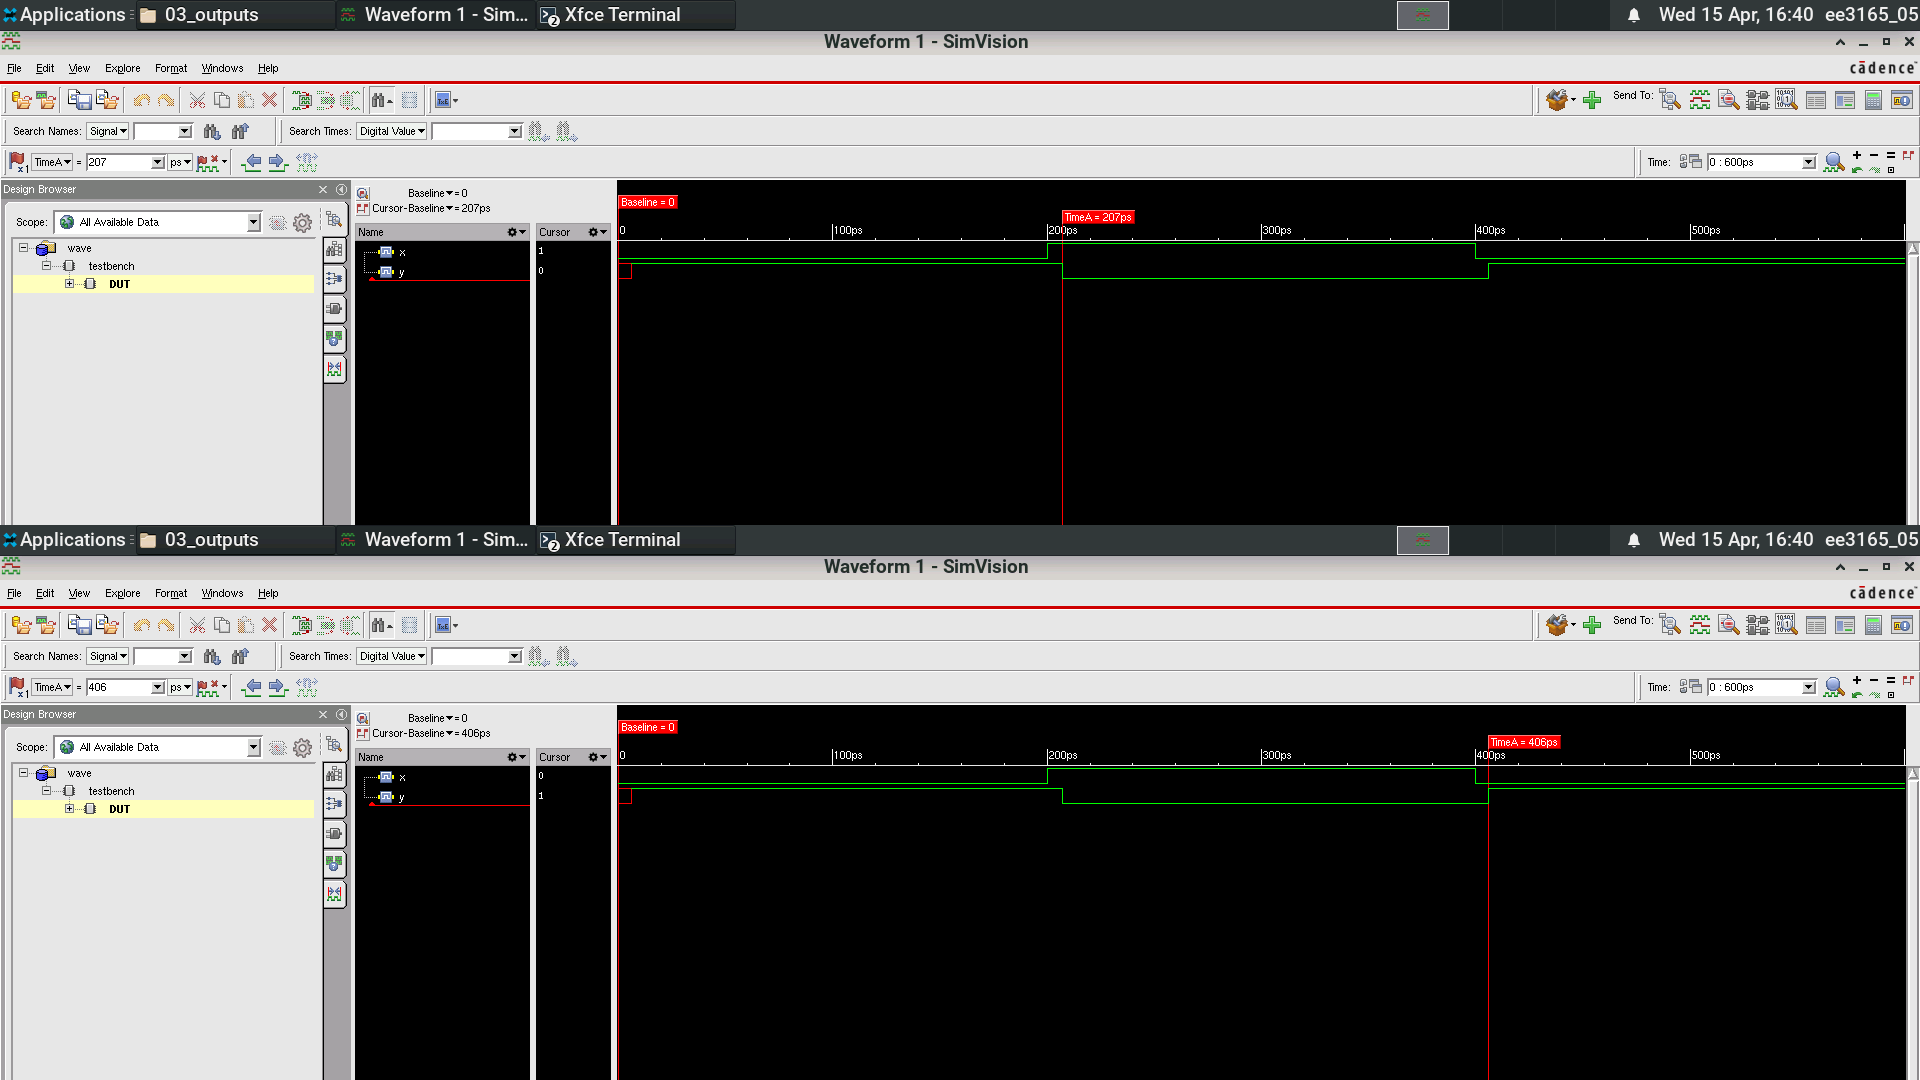
\includegraphics[width=\textwidth]{figures/exp1_lvt_not_slow_1v0.png}
        \caption{Corner LVT Slow (slow\_vdd1v0)}
        \label{fig:not_lvt_slow}
    \end{subfigure}
    
    \caption{Waveform đo độ trễ cổng NOT sử dụng thư viện LVT. Quan sát thấy độ trễ được cải thiện đáng kể so với thư viện HVT ở cùng điều kiện vận hành.}
    \label{fig:not_lvt_comparison}
\end{figure}

\textbf{Nhận xét:} Đối với thư viện Low Threshold Voltage (LVT), khi hoạt động ở cùng mức điện áp suy giảm 1.0V, mạch thể hiện những ưu điểm khác biệt:
\begin{itemize}
    \item \textbf{Khả năng duy trì tốc độ:} Nhờ có điện áp ngưỡng ($V_{th}$) thấp, điện áp quá lái ($V_{OV}$) của các transistor LVT vẫn được duy trì ở mức đủ lớn ngay cả khi $V_{DD}$ chỉ còn 1.0V. Do đó, dòng $I_{on}$ vẫn đáp ứng tốt cho việc chuyển mạch nhanh.
    \item \textbf{Cải thiện độ trễ so với HVT:} So chiếu với HVT tại cùng góc \texttt{slow\_vdd1v0}, cổng NOT dùng thư viện LVT chỉ mất $0.012ns$ (nhanh hơn $20\%$). Điều này chứng minh LVT là "cứu cánh" tuyệt vời cho các đường dẫn tới hạn khi thiết kế phải ép xung trong chế độ điện áp thấp.
    \item \textbf{Sự đánh đổi về công suất:} Mặc dù chạy ở 1.0V, các cell LVT vẫn tiêu tốn nhiều năng lượng hơn so với HVT (ví dụ tại \texttt{slow\_vdd1v0\_lvt} là $5.48 \times 10^{-9}$ W). Nguyên nhân là do $V_{th}$ thấp khiến dòng rò rỉ qua kênh dẫn luôn ở mức cao ngay cả khi transistor ở trạng thái tắt.
\end{itemize}

Mô phỏng tại góc điện áp 1.2V cho thư viện Low Threshold Voltage (LVT) nhằm xác định giới hạn tốc độ tối đa của linh kiện.

\begin{figure}[H]
    \centering
    % --- Hình bên trái: LVT Fast ---
    \begin{subfigure}[b]{0.48\textwidth}
        \centering
        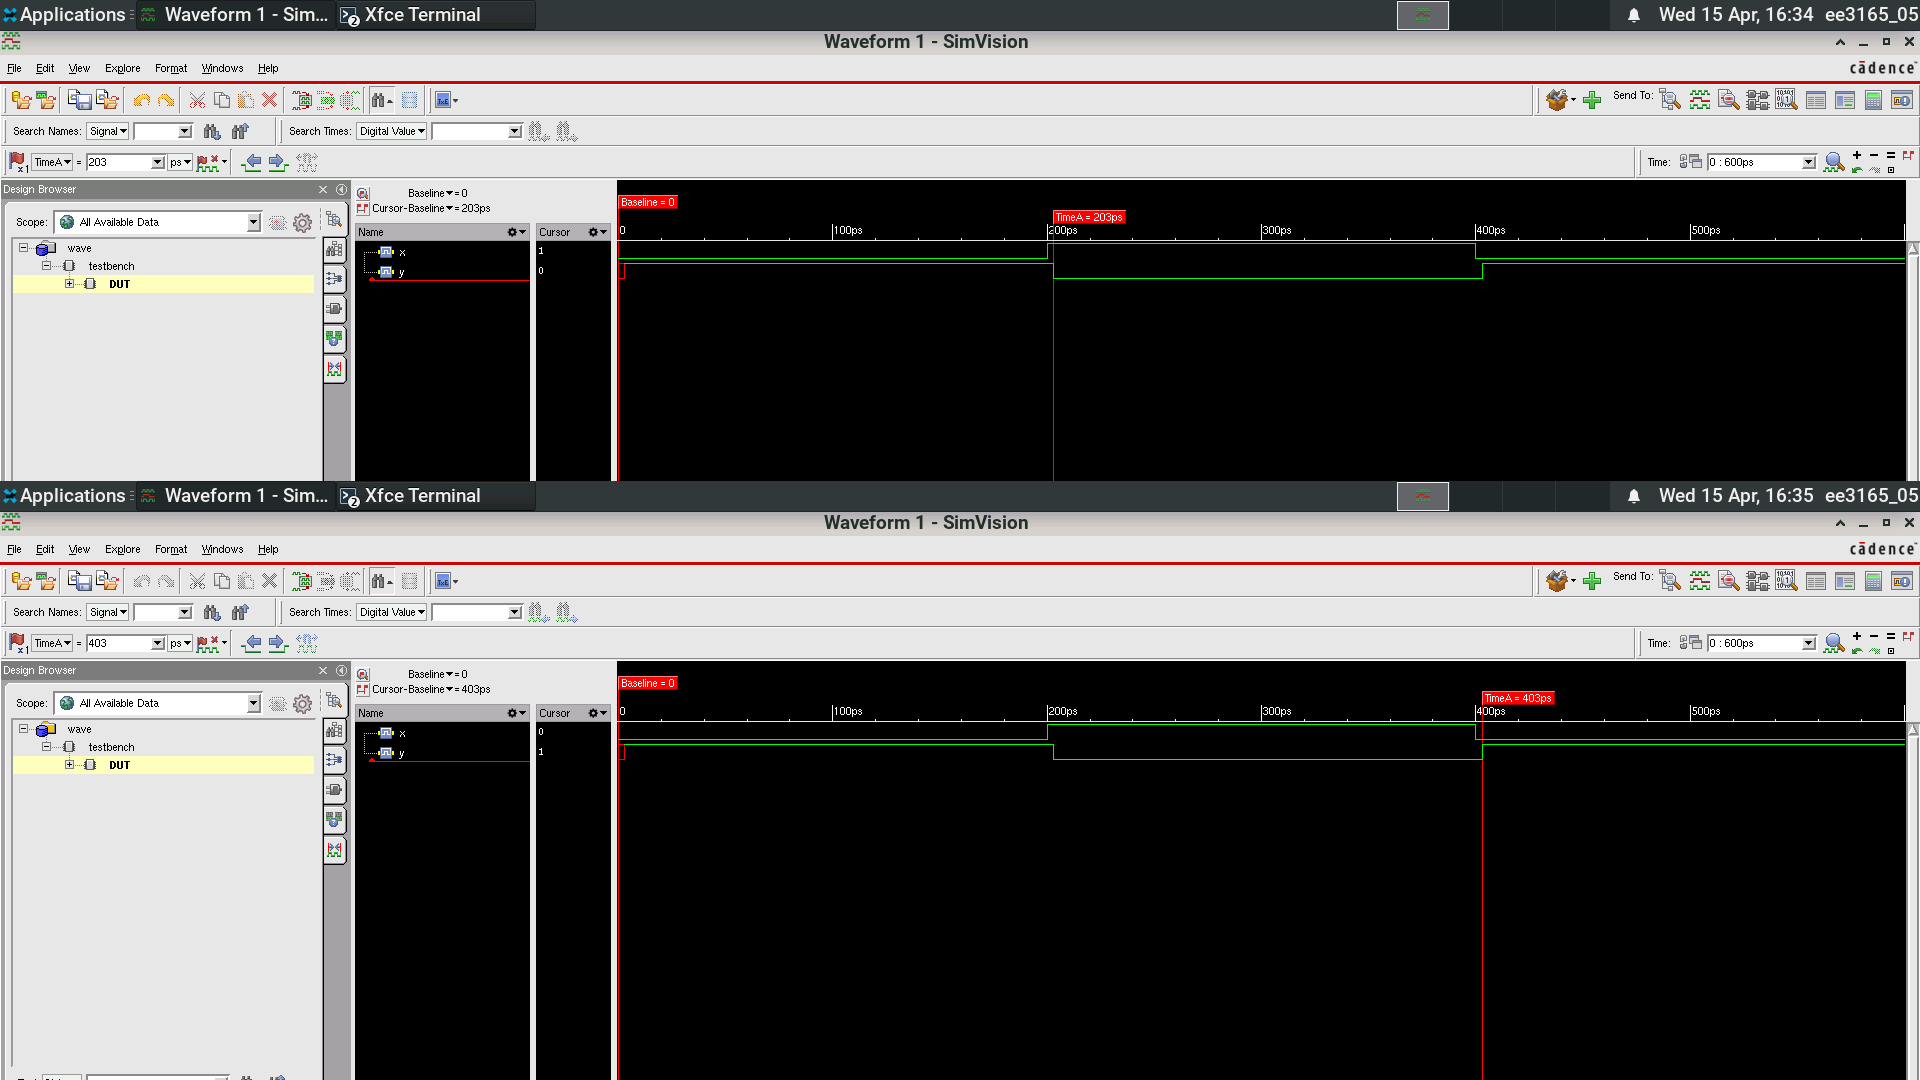
\includegraphics[width=\textwidth]{figures/exp1_lvt_not_fast_1v2.png}
        \caption{Corner LVT Fast (fast\_vdd1v2)}
        \label{fig:not_lvt_fast}
    \end{subfigure}
    \hfill
    % --- Hình bên phải: LVT Slow ---
    \begin{subfigure}[b]{0.48\textwidth}
        \centering
        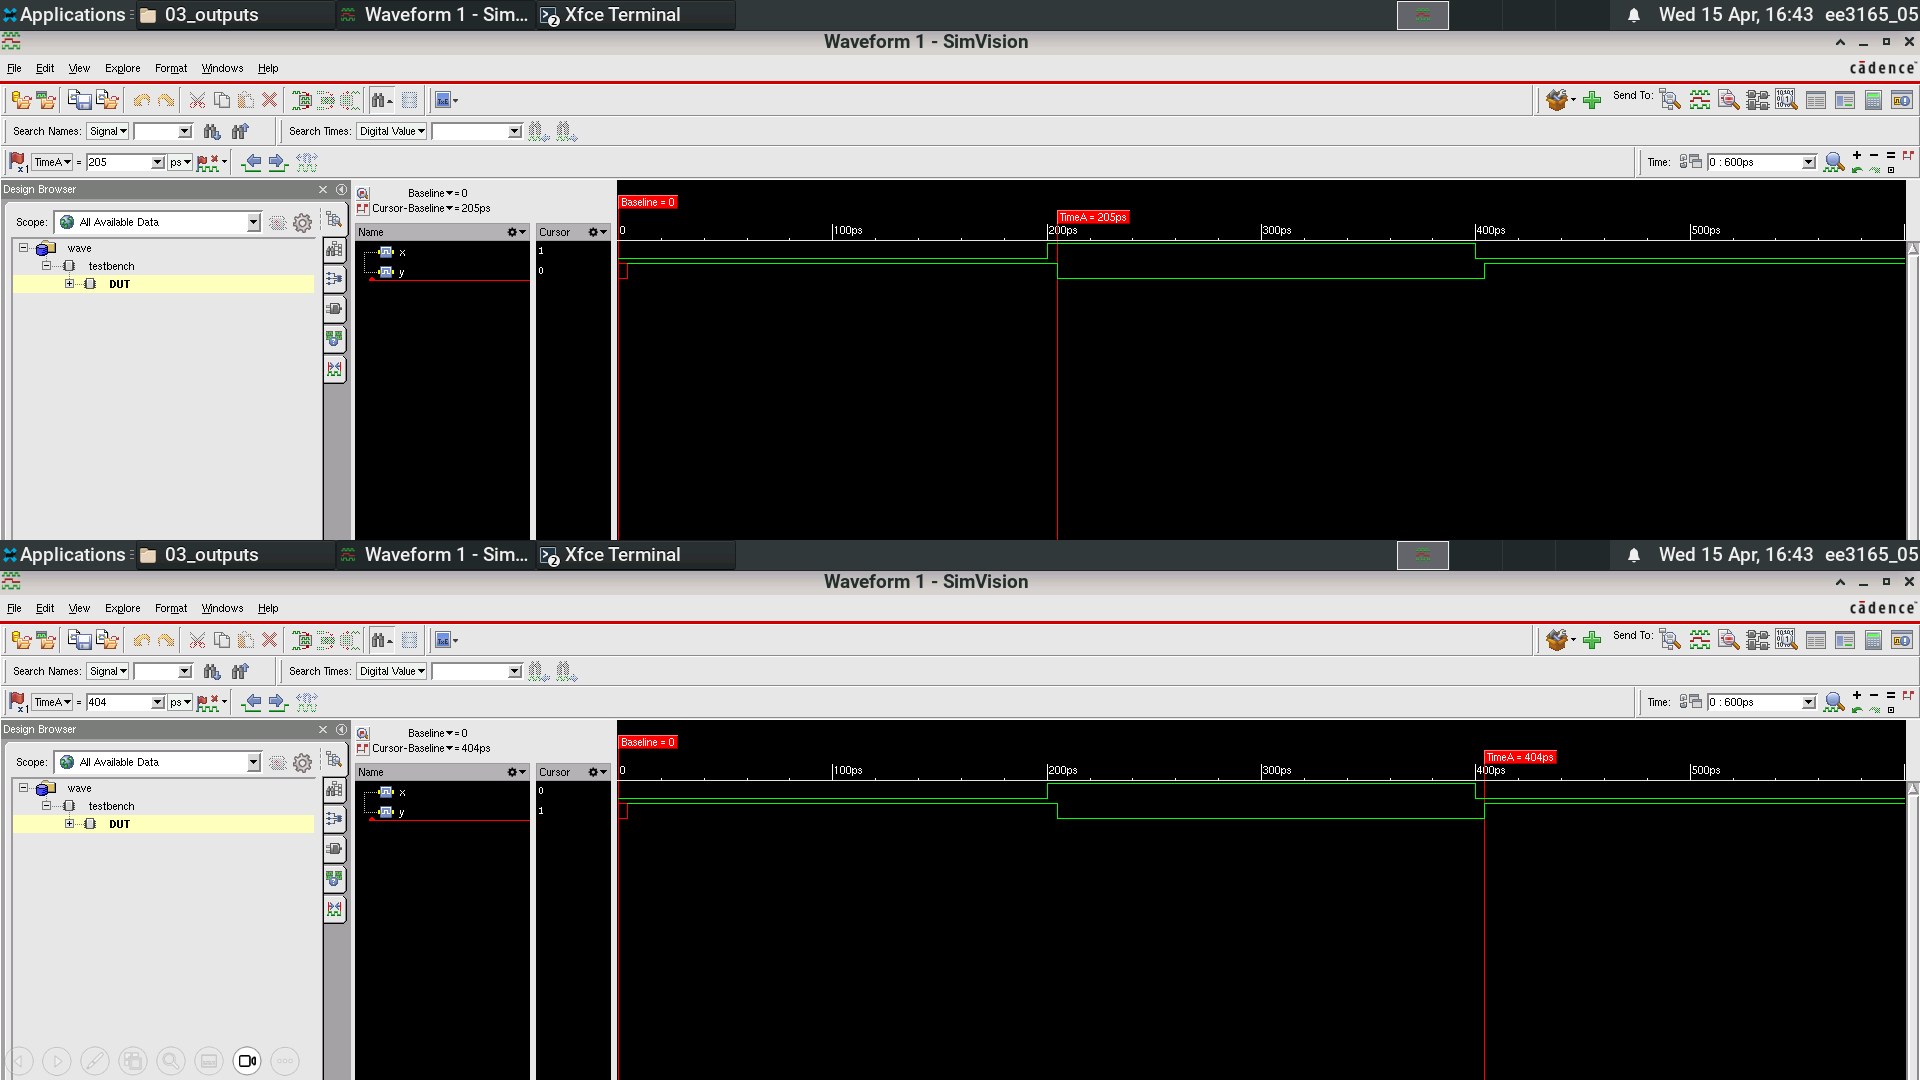
\includegraphics[width=\textwidth]{figures/exp1_lvt_not_slow_1v2.png}
        \caption{Corner LVT Slow (slow\_vdd1v2)}
        \label{fig:not_lvt_slow}
    \end{subfigure}
    
    \caption{Waveform đo độ trễ cổng NOT sử dụng thư viện LVT với VDD=1.2V}
    \label{fig:not_lvt_comparison}
\end{figure}

\textbf{Nhận xét đặc tính LVT tại 1.2V:}
\begin{itemize}
    \item \textbf{Tốc độ cực hạn:} Sự kết hợp giữa $V_{th}$ thấp và $V_{DD}$ cao tạo ra dòng $I_{on}$ cực đại. Đây là điều kiện giúp cổng NOT đạt độ trễ thấp nhất trong 8 corners khảo sát ($t_{pd}$ tối thiểu). Sườn xung ($t_{rise}, t_{fall}$) rất dốc, cho thấy khả năng chuyển mạch cực nhanh.
    \item \textbf{Đánh đổi về dòng rò:} Tại mức 1.2V, nhược điểm của LVT bộc lộ rõ nhất qua công suất rò rỉ tăng vọt. Do rào cản điện áp thấp, dòng rò dưới ngưỡng tăng mạnh khi điện áp nguồn cao. Thư viện này tại 1.2V chỉ nên dùng cho các đường dẫn tới hạn để giải quyết các vi phạm về thời gian nghiêm trọng.
\end{itemize}

\paragraph{C. Kết luận} 

Từ việc phân tích chéo dữ liệu của 8 process corners (bao gồm sự biến thiên về quy trình, điện áp và loại thư viện), nhóm rút ra các kết luận tổng thể mang tính quy luật đối với thiết kế vi mạch số như sau:

\begin{itemize}
    \item \textbf{Bài toán đánh đổi Thư viện (HVT vs. LVT):} Việc lựa chọn thư viện là sự đánh đổi trực tiếp giữa Tốc độ và Công suất tĩnh. Thư viện LVT mang lại hiệu năng chuyển mạch xuất sắc nhưng gây ra tổn hao năng lượng lớn do dòng rò dưới ngưỡng. Ngược lại, HVT hi sinh tốc độ để đạt được độ tối ưu tuyệt đối về năng lượng tĩnh. Trong thực tế tổng hợp mạch, công cụ sẽ ưu tiên dùng HVT cho phần lớn thiết kế và chỉ chèn LVT vào các đường dẫn tới hạn.
    
    \item \textbf{Bài toán đánh đổi Điện áp (1.2V vs. 1.0V):} Điện áp cung cấp ($V_{DD}$) là đòn bẩy mạnh nhất để điều chỉnh hiệu năng. Hạ áp xuống 1.0V mang lại lợi ích to lớn về giảm công suất động ($P_{dyn} \propto V_{DD}^2$), nhưng lại khiến mạch đối mặt với rủi ro trễ thời gian do dòng bão hòa ($I_{on}$) bị thu hẹp, đặc biệt là hiện tượng "đói dòng" ở các cell HVT.
    
    \item \textbf{Tầm quan trọng của phân tích đa góc:} Sự chênh lệch độ trễ từ $0.002ns$ (ở \texttt{fast\_vdd1v2\_lvt}) lên đến $0.015ns$ (ở \texttt{slow\_vdd1v0\_hvt}) minh chứng rõ ràng cho sự cần thiết của việc kiểm tra toàn diện. Góc Fast xác định giới hạn về Công suất và Hold time, trong khi góc Slow quyết định tần số hoạt động tối đa của mạch và kiểm tra vi phạm Setup time.
\end{itemize}

\textbf{Tổng kết:} Đặc tính của cổng NOT – cũng như bất kỳ Standard Cell nào khác – không phải là một hằng số mà là một hàm phụ thuộc mạnh mẽ vào điều kiện PVT (Process, Voltage, Temperature) và công nghệ chế tạo. Việc nắm vững các quy luật này là cơ sở cốt lõi để thực hiện bước tổng hợp mức cổng đạt chuẩn PPA (Power - Performance - Area).

\newpage
\subsubsection{OR2}
\begin{lstlisting}[style={prettyverilog}, caption={\texttt{code thiết kế cổng OR}}]
`timescale 1ns/1ps
module or(
    input logic A,
    input logic B,
      output logic Y);
    assign Y = A | B;
endmodule
\end{lstlisting}
\begin{lstlisting}[style={prettyverilog}, caption={\texttt{code testbench cổng OR}}]
`timescale 1ns/1ps
module tb_or;
    logic A, B;
    logic Y;
    or(.A(A), .B(B), .Y(Y));
    initial begin
        $dumpfile("or_wave.vcd");
        $dumpvars(0, tb_or);
        A = 0; B = 0; #10;
        A = 0; B = 1; #10;
        A = 0; B = 0; #10;
        A = 1; B = 0; #10;
        A = 0; B = 0; #10;
        $finish;
    end
endmodule
\end{lstlisting}

Trước hết, để tổng quan về linh kiện, Hình \ref{fig:exp1_or2} trình bày ký hiệu logic cơ bản của cổng OR2. Linh kiện này có hai ngõ vào A, B và một ngõ ra Y, thực hiện phương trình đại số Boole $Y = A + B$ (ngõ ra chỉ ở mức 0 khi cả hai ngõ vào đều ở mức 0).

\begin{figure}[H]
    \centering
    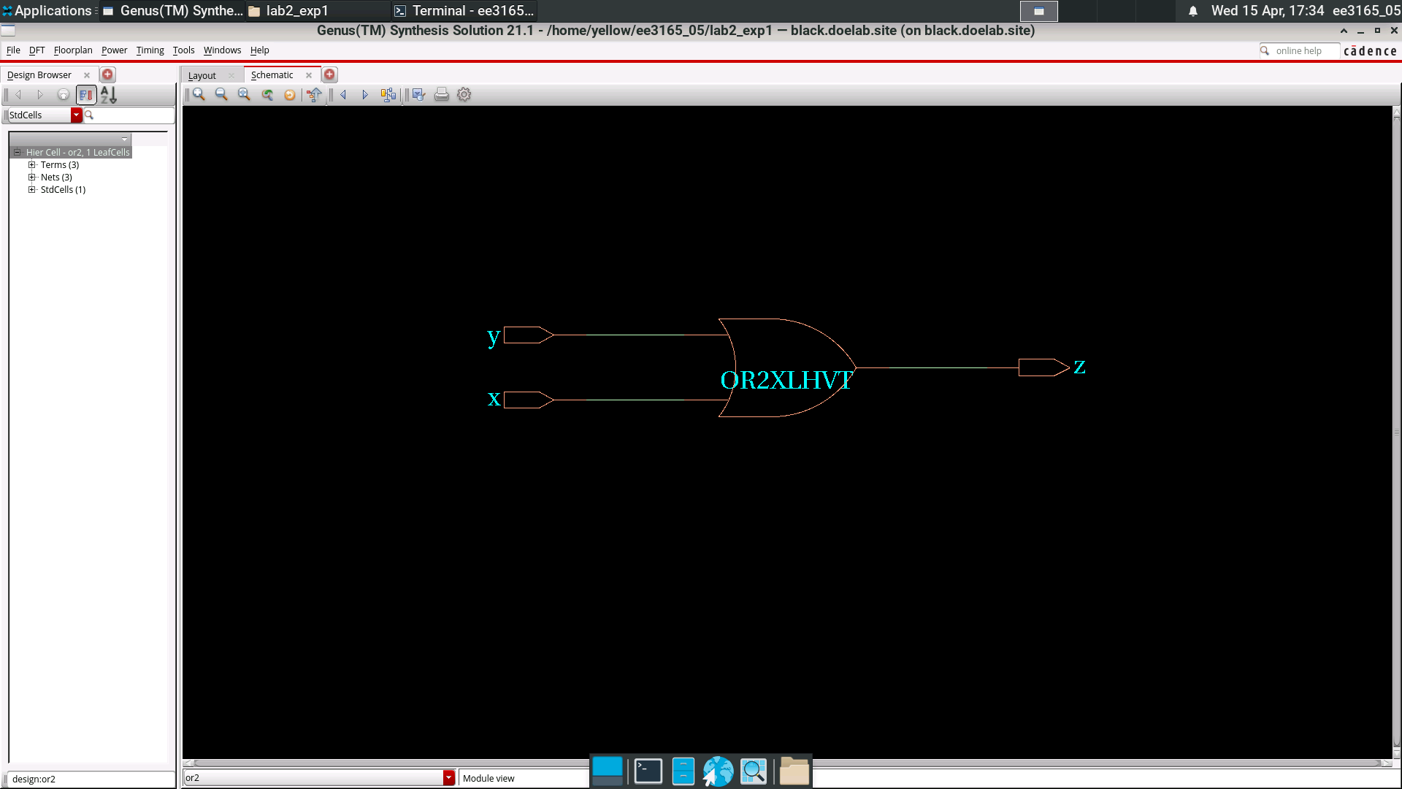
\includegraphics[width=0.6\textwidth]{figures/exp1_or2.png}
    \caption{Ký hiệu schematic và đặc tính logic cơ bản của cổng OR2.}
    \label{fig:exp1_or2}
\end{figure}

Sau khi viết mã RTL, thiết kế được đưa vào công cụ Genus để thực hiện quá trình tổng hợp. Hình \ref{fig:exp1_or2_mapped} minh họa sơ đồ mức cổng của cổng OR2. Hình ảnh này là minh chứng cho việc công cụ đã biên dịch và ánh xạ thành công module mức RTL thành một Standard Cell vật lý cụ thể trong thư viện 45nm.

\begin{figure}[H]
    \centering
    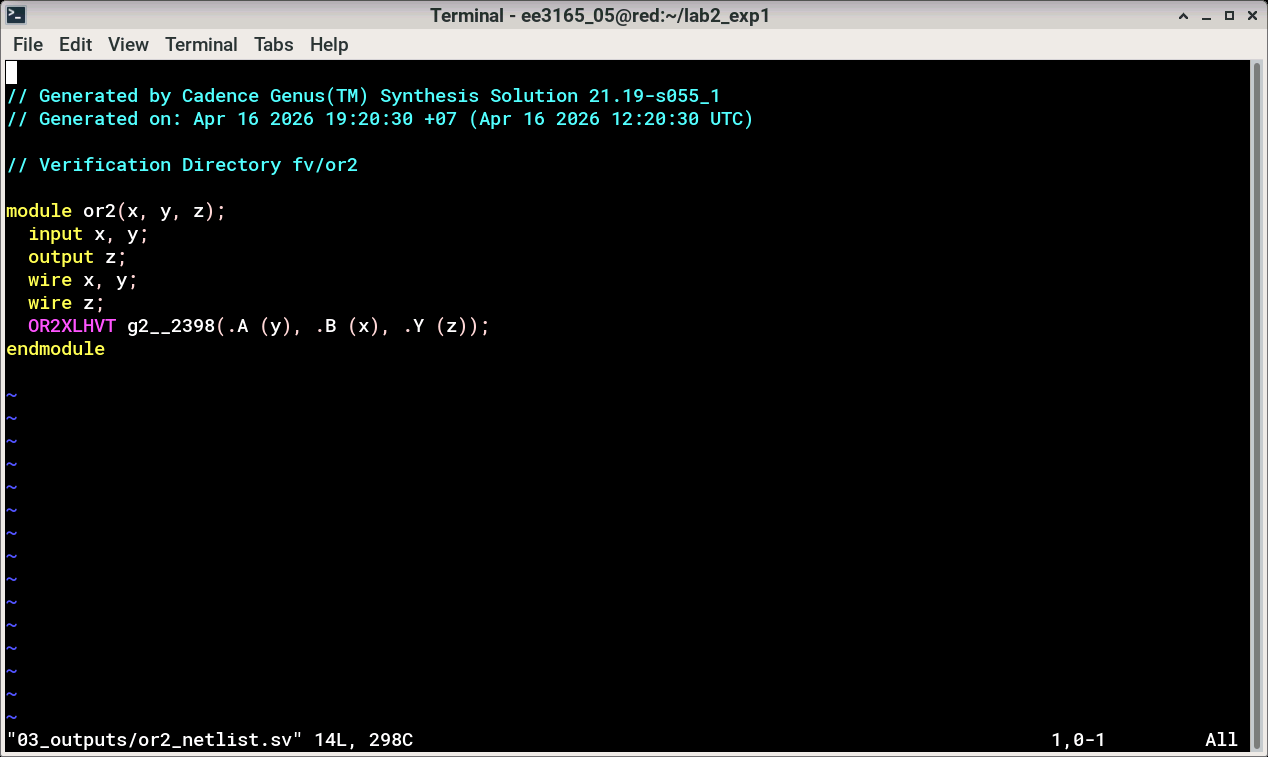
\includegraphics[width=0.7\textwidth]{figures/exp1_or2_mapped.png}
    \caption{Sơ đồ mức cổng của thiết kế OR2 hiển thị trên giao diện Genus sau bước tổng hợp.}
    \label{fig:exp1_or2_mapped}
\end{figure}

Nhóm tiếp tục thực hiện khảo sát đặc tính của cổng OR2 trên cả hai loại thư viện: High Threshold Voltage (HVT) và Low Threshold Voltage (LVT) để đánh giá sự đánh đổi giữa tốc độ và công suất.

\paragraph{A. Thư viện High Threshold Voltage (HVT)}
Đặc tính của các cell HVT là dòng rò thấp nhưng độ trễ lớn hơn. Kết quả mô phỏng 8 corners được tổng hợp trong bảng dưới đây:

\begin{table}[H]
\centering
\renewcommand{\arraystretch}{1.3}
\resizebox{\textwidth}{!}{
\begin{tabular}{|l|c|c|c|c|c|c|}
\hline
\multirow{2}{*}{\textbf{Library Name}} 
& \multirow{2}{*}{\textbf{Total Area}} 
& \multirow{2}{*}{\textbf{Total Power}} 
& \multicolumn{2}{c|}{\textbf{Delay A$\rightarrow$Y}} 
& \multicolumn{2}{c|}{\textbf{Delay B$\rightarrow$Y}} \\
\cline{4-7}
& & 
& \textbf{Rising (ns)} & \textbf{Falling (ns)}
& \textbf{Rising (ns)} & \textbf{Falling (ns)} \\
\hline
 
% ----------- KHỐI HVT ----------------
fast\_vdd1v0\_basicCells\_hvt & 1.368 & 1.73733e-08 & 0.017 & 0.029 & 0.015 & 0.026 \\ \hline
fast\_vdd1v2\_basicCells\_hvt & 1.368 & 2.53194e-08 & 0.013 & 0.021 & 0.011 & 0.019 \\ \hline
slow\_vdd1v0\_basicCells\_hvt & 1.368 & 1.14746e-08 & 0.077 & 0.099 & 0.065 & 0.088 \\ \hline
slow\_vdd1v2\_basicCells\_hvt & 1.368 & 1.68838e-08 & 0.037 & 0.050 & 0.031 & 0.044 \\ \hline
 
\end{tabular}
}
\caption{Tổng hợp thông số Diện tích, Công suất và Độ trễ của cổng OR2 qua 8 process corners (HVT).}
\label{tab:exp1_or2_hvt_params}
\end{table}

Dưới đây là sự so sánh dạng sóng mô phỏng của cổng OR2 tại hai góc cực đoan: Fast (nhanh nhất) và Slow (chậm nhất) ở cùng mức điện áp 1.0V.

\begin{figure}[H]
    \centering
    % --- Hình bên trái: Corner Fast ---
    \begin{subfigure}[b]{0.48\textwidth}
        \centering
        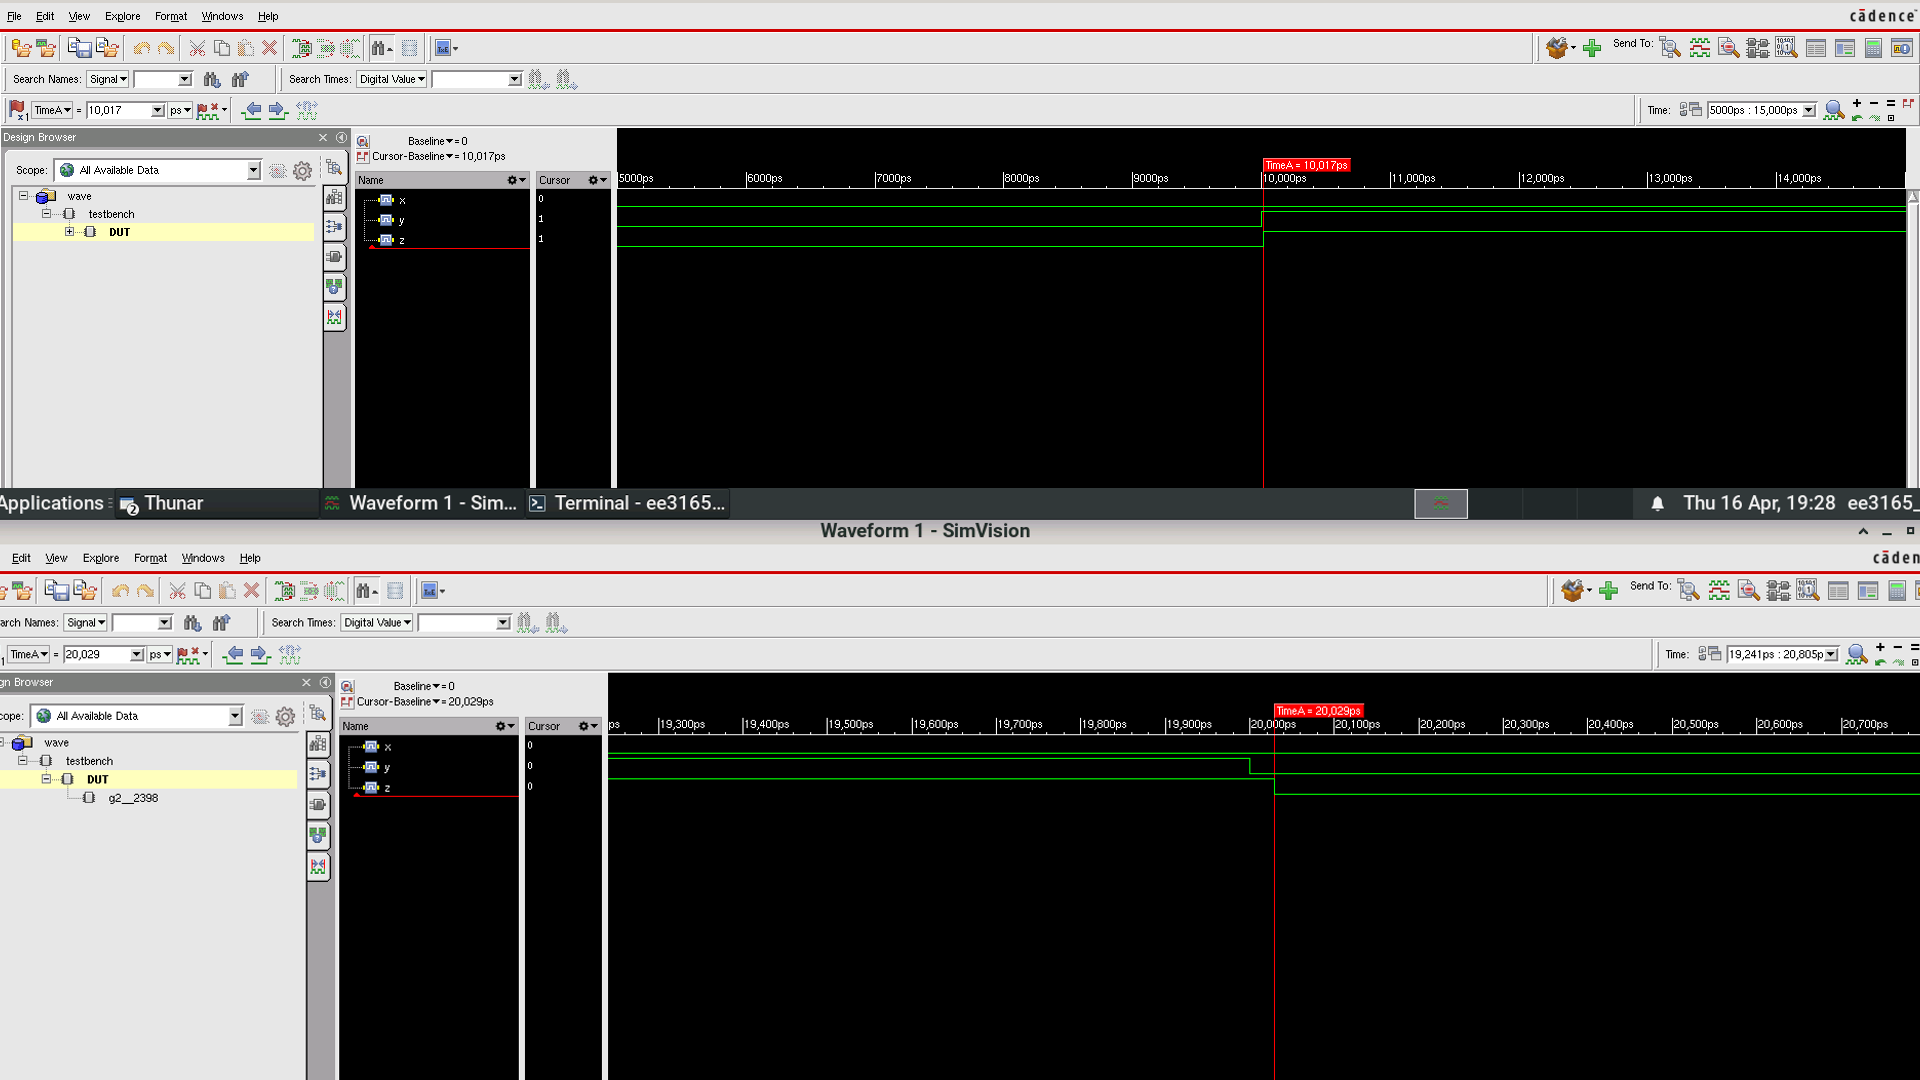
\includegraphics[width=\textwidth]{figures/exp1_or2_hvt_fast_1v0.png}
        \caption{Corner HVT Fast (fast\_vdd1v0)}
        \label{fig:or2_hvt_fast_1v0}
    \end{subfigure}
    \hfill
    % --- Hình bên phải: Corner Slow ---
    \begin{subfigure}[b]{0.48\textwidth}
        \centering
        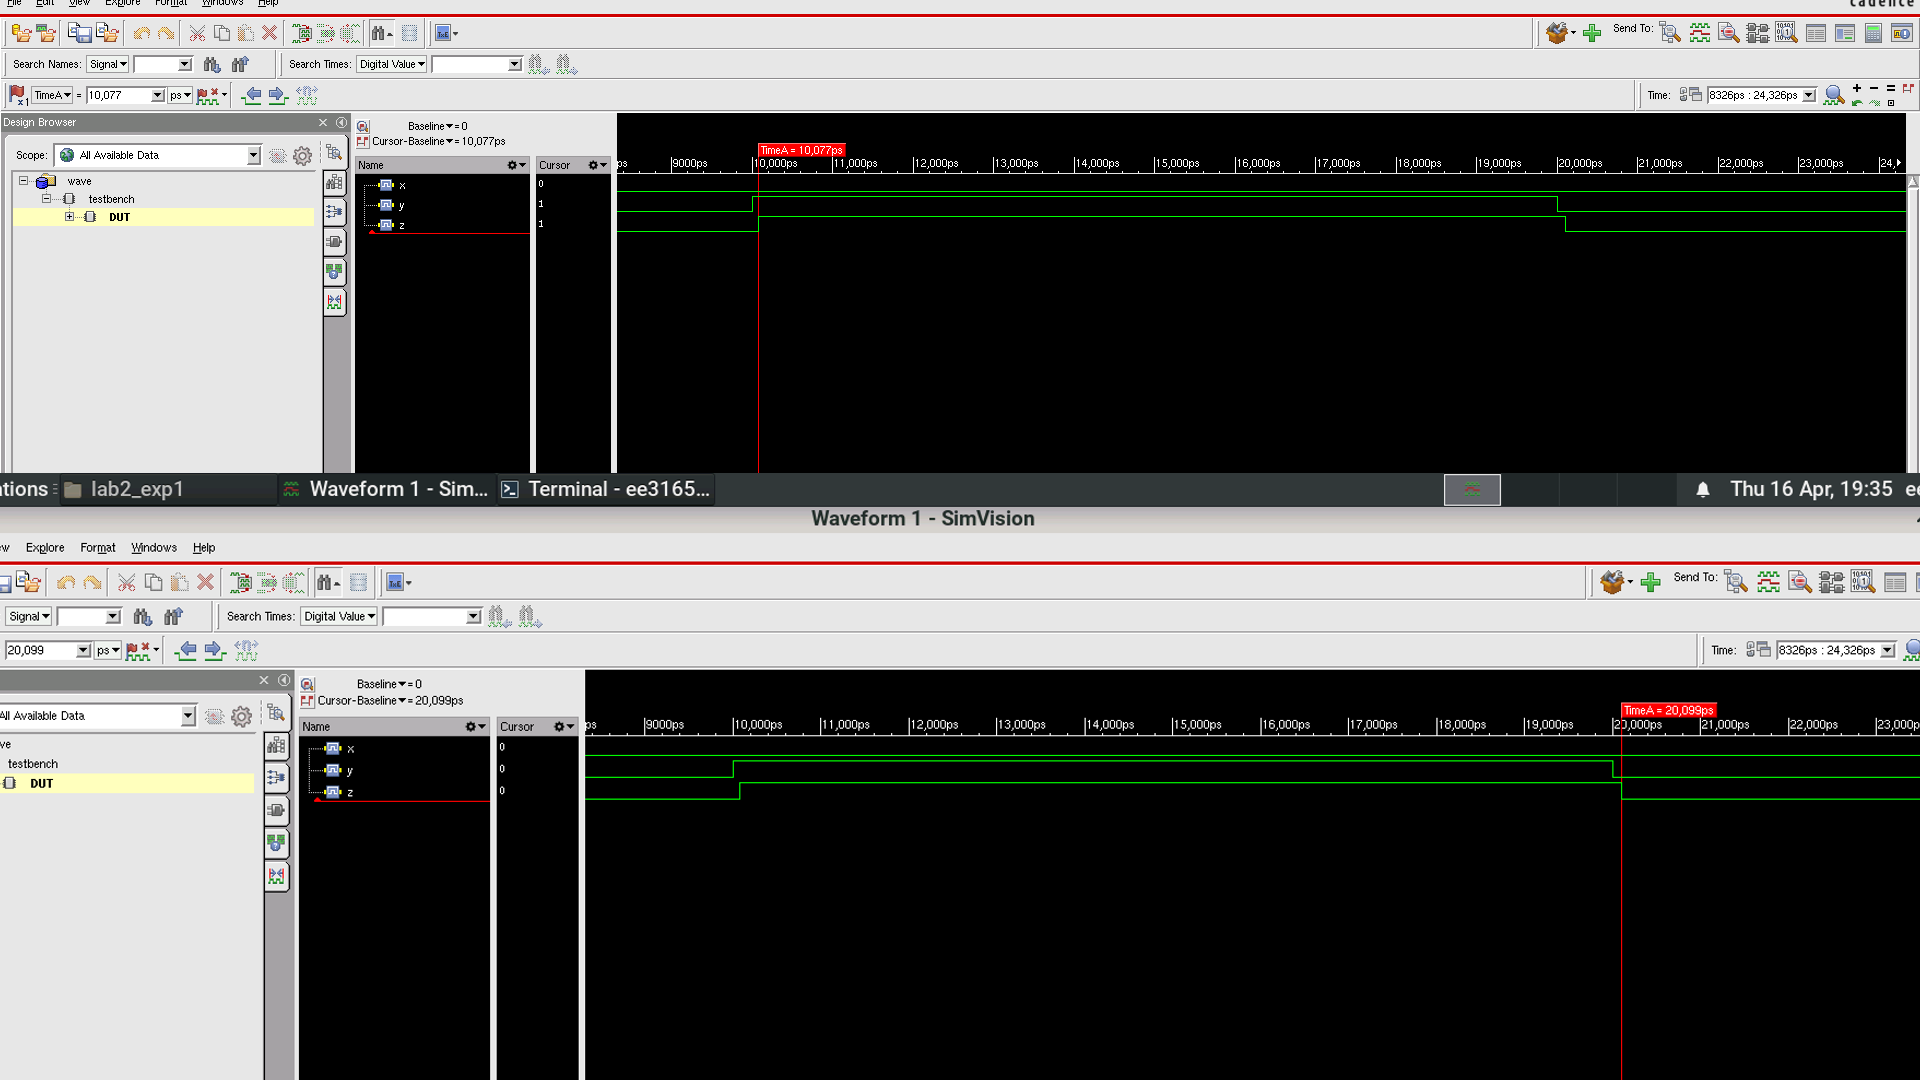
\includegraphics[width=\textwidth]{figures/exp1_or2_hvt_slow_1v0.png}
        \caption{Corner HVT Slow (slow\_vdd1v0)}
        \label{fig:or2_hvt_slow_1v0}
    \end{subfigure}
    
    \caption{So sánh Waveform đo độ trễ cổng OR2 ở High Threshold Voltage. Lưu ý sự khác biệt về độ dốc của sườn tín hiệu và giá trị Delta T (độ trễ) giữa hai trường hợp.}
    \label{fig:or2_comparison_1v0}
\end{figure}

\textbf{Nhận xét (HVT - 1.0V):} Quan sát dữ liệu đo đạc tại mức điện áp suy giảm 1.0V, ta rút ra các kết luận vật lý sau:
\begin{itemize}
    \item \textbf{Suy giảm tốc độ do đói dòng:} Tại góc khắc nghiệt nhất \texttt{slow\_vdd1v0\_hvt}, dòng bão hòa $I_{on}$ bị bóp nghẹt khiến độ trễ sườn xuống của chân A đạt mức cực đại $0.099ns$. Đây là worst-case bắt buộc phải xem xét để tránh vi phạm Setup Time.
    \item \textbf{Đặc tính bất đối xứng của ngõ vào:} Bảng dữ liệu cho thấy độ trễ \texttt{A$\rightarrow$Y} luôn lớn hơn \texttt{B$\rightarrow$Y} (ví dụ: $0.099ns$ so với $0.088ns$). Điều này phản ánh thực tế kiến trúc Layout của Standard Cell, nơi vị trí các transistor nối tiếp/song song đối với từng chân ngõ vào tạo ra điện dung ký sinh khác nhau.
    \item \textbf{Tối ưu hóa năng lượng tĩnh:} Bù lại nhược điểm tốc độ, góc chậm nhất ở 1.0V mang lại công suất tiêu thụ cực kỳ ấn tượng, chạm mức thấp kỷ lục chỉ $1.147 \times 10^{-8}W$.
\end{itemize}

Dưới đây là kết quả mô phỏng dạng sóng của cổng OR2 sử dụng thư viện High Threshold Voltage (HVT) tại điều kiện điện áp danh định 1.2V.

\begin{figure}[H]
    \centering
    % --- Hình bên trái: Corner Fast ---
    \begin{subfigure}[b]{0.48\textwidth}
        \centering
        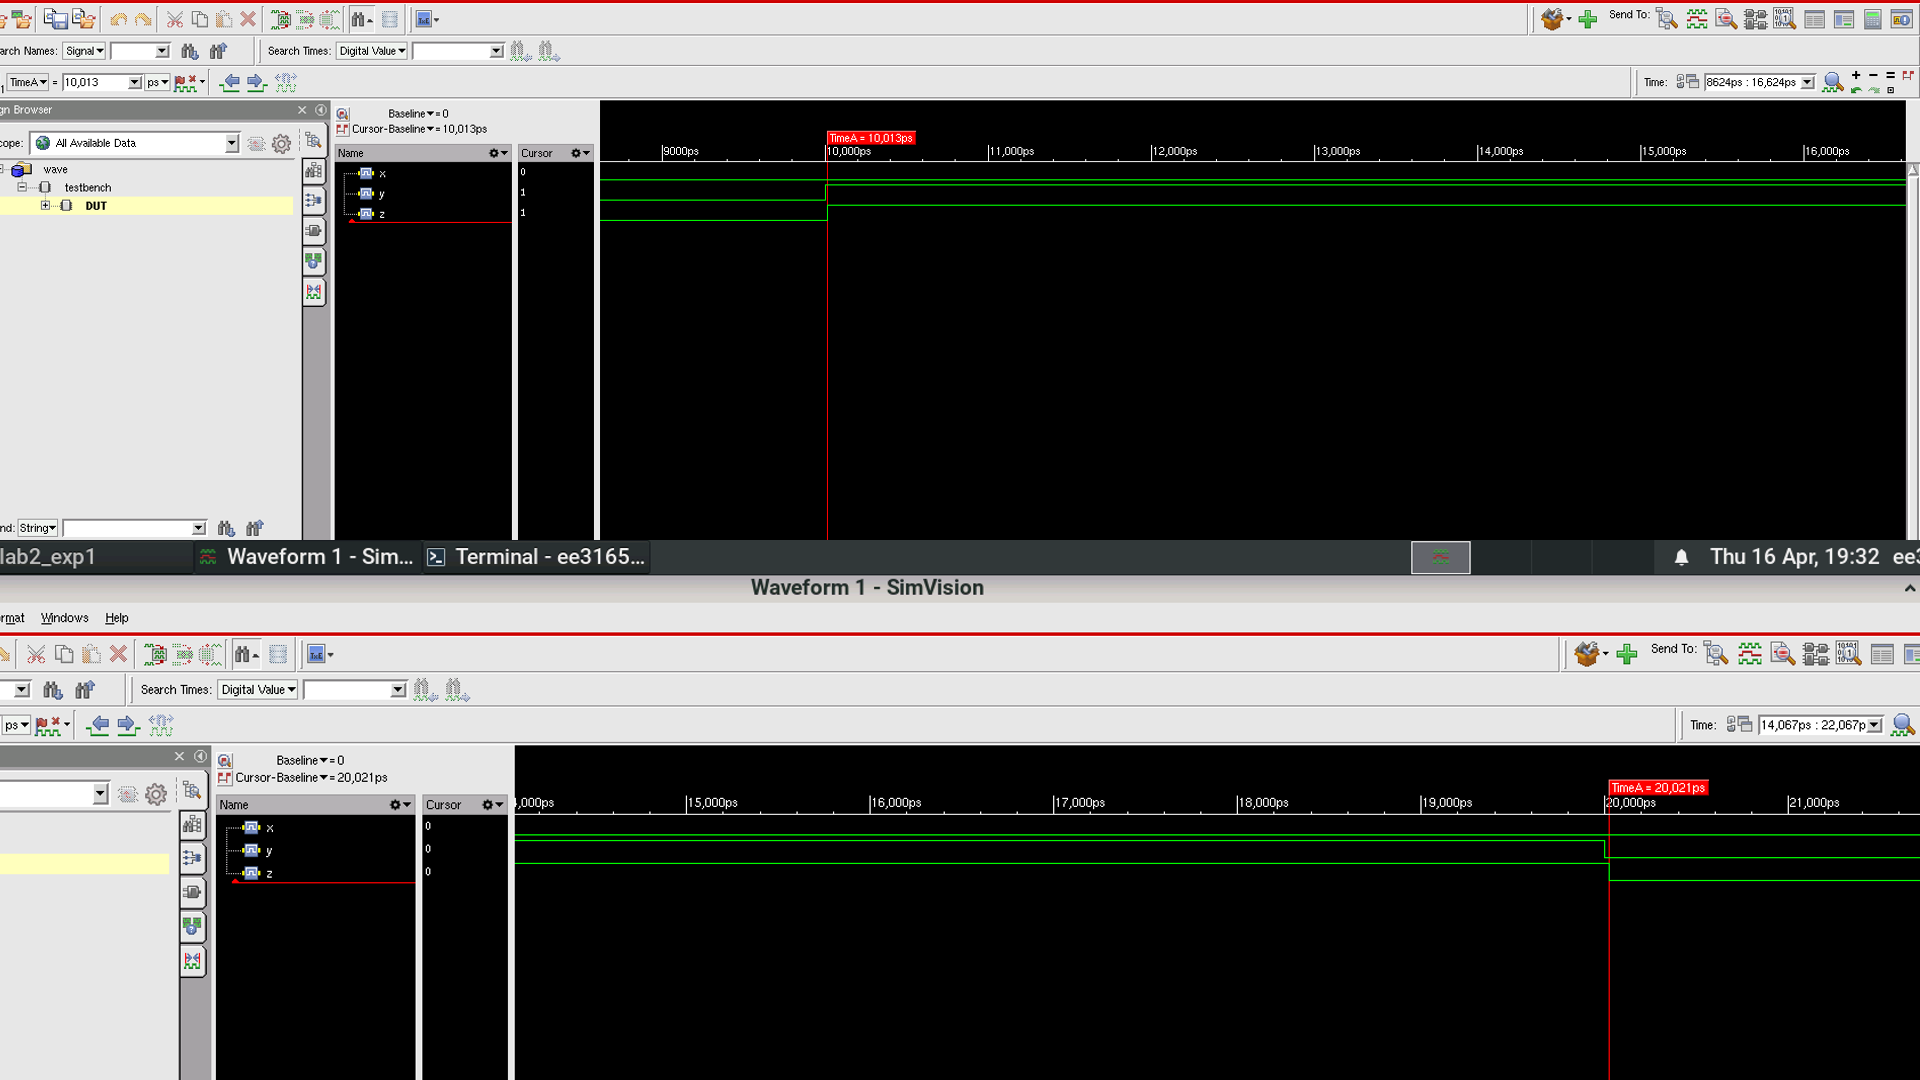
\includegraphics[width=\textwidth]{figures/exp1_or2_hvt_fast_1v2.png}
        \caption{Corner HVT Fast (fast\_vdd1v2)}
        \label{fig:or2_hvt_fast_1v2}
    \end{subfigure}
    \hfill
    % --- Hình bên phải: Corner Slow ---
    \begin{subfigure}[b]{0.48\textwidth}
        \centering
        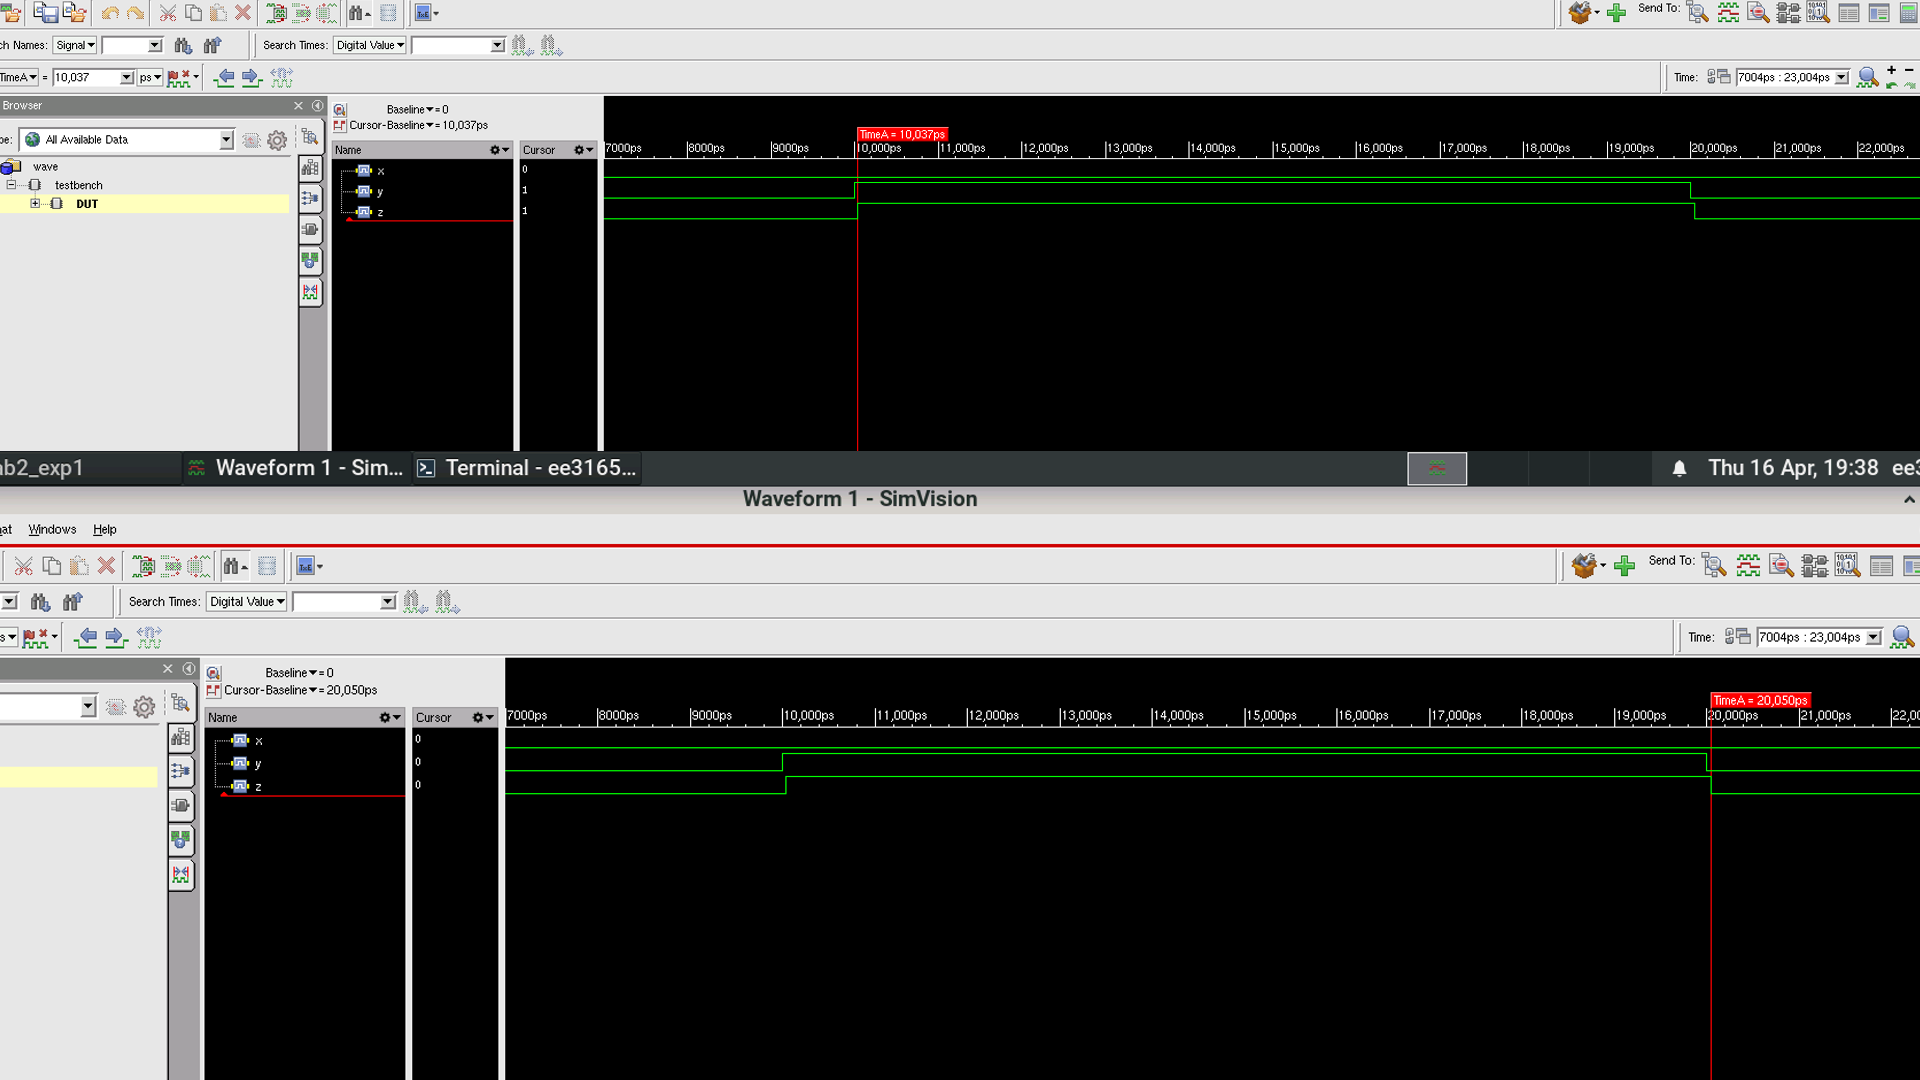
\includegraphics[width=\textwidth]{figures/exp1_or2_hvt_slow_1v2.png}
        \caption{Corner HVT Slow (slow\_vdd1v2)}
        \label{fig:or2_hvt_slow_1v2}
    \end{subfigure}
    \caption{So sánh Waveform đo độ trễ cổng OR2 ở High Threshold Voltage với VDD = 1.2V}
    \label{fig:or2_comparison_1v2}
\end{figure}

\textbf{Nhận xét (HVT - 1.2V):} Việc nâng điện áp cung cấp lên mức danh định 1.2V giúp cấu trúc HVT cải thiện đáng kể hiệu năng:
\begin{itemize}
    \item \textbf{Cải thiện tốc độ:} Điện áp quá lái ($V_{OV}$) tăng giúp độ trễ giảm hơn một nửa so với 1.0V. Ở góc \texttt{fast\_vdd1v2\_hvt}, Rising Delay của ngõ B chỉ còn $0.011ns$.
    \item \textbf{Gia tăng công suất động:} Đổi lại, tổng công suất ở góc Fast tăng vọt lên $2.53 \times 10^{-8}W$, minh chứng cho định luật công suất động tỷ lệ thuận với bình phương điện áp nguồn ($P_{dyn} \propto V_{DD}^2$).
\end{itemize}

\paragraph{B. Thư viện Low Threshold Voltage (LVT)}

Ngược lại, các cell LVT cho tốc độ chuyển mạch cực nhanh nhờ điện áp ngưỡng thấp, nhưng yêu cầu đánh đổi bằng mức tiêu hao năng lượng lớn hơn.

\begin{table}[H]
\centering
\renewcommand{\arraystretch}{1.3}
\resizebox{\textwidth}{!}{
\begin{tabular}{|l|c|c|c|c|c|c|}
\hline
\multirow{2}{*}{\textbf{Library Name}} 
& \multirow{2}{*}{\textbf{Total Area}} 
& \multirow{2}{*}{\textbf{Total Power}} 
& \multicolumn{2}{c|}{\textbf{Delay A$\rightarrow$Y}} 
& \multicolumn{2}{c|}{\textbf{Delay B$\rightarrow$Y}} \\
\cline{4-7}
& & 
& \textbf{Rising (ns)} & \textbf{Falling (ns)}
& \textbf{Rising (ns)} & \textbf{Falling (ns)} \\
\hline
 
% ----------- KHỐI LVT ----------------
fast\_vdd1v0\_basicCells\_lvt & 1.368 & 2.23841e-08 & 0.011 & 0.017 & 0.009 & 0.015 \\ \hline
fast\_vdd1v2\_basicCells\_lvt & 1.368 & 3.34466e-08 & 0.009 & 0.014 & 0.008 & 0.012 \\ \hline
slow\_vdd1v0\_basicCells\_lvt & 1.368 & 1.26400e-08 & 0.033 & 0.052 & 0.027 & 0.045 \\ \hline
slow\_vdd1v2\_basicCells\_lvt & 1.368 & 1.84242e-08 & 0.022 & 0.034 & 0.018 & 0.030 \\ \hline
 
\end{tabular}
}
\caption{Tổng hợp thông số Diện tích, Công suất và Độ trễ của OR2 (Thư viện LVT).}
\label{tab:exp1_lvt_or2_params}
\end{table}

Sau khi khảo sát thư viện HVT, nhóm tiếp tục thực hiện mô phỏng với thư viện LVT để đánh giá sự cải thiện về tốc độ.

\begin{figure}[H]
    \centering
    % --- Hình bên trái: LVT Fast ---
    \begin{subfigure}[b]{0.48\textwidth}
        \centering
        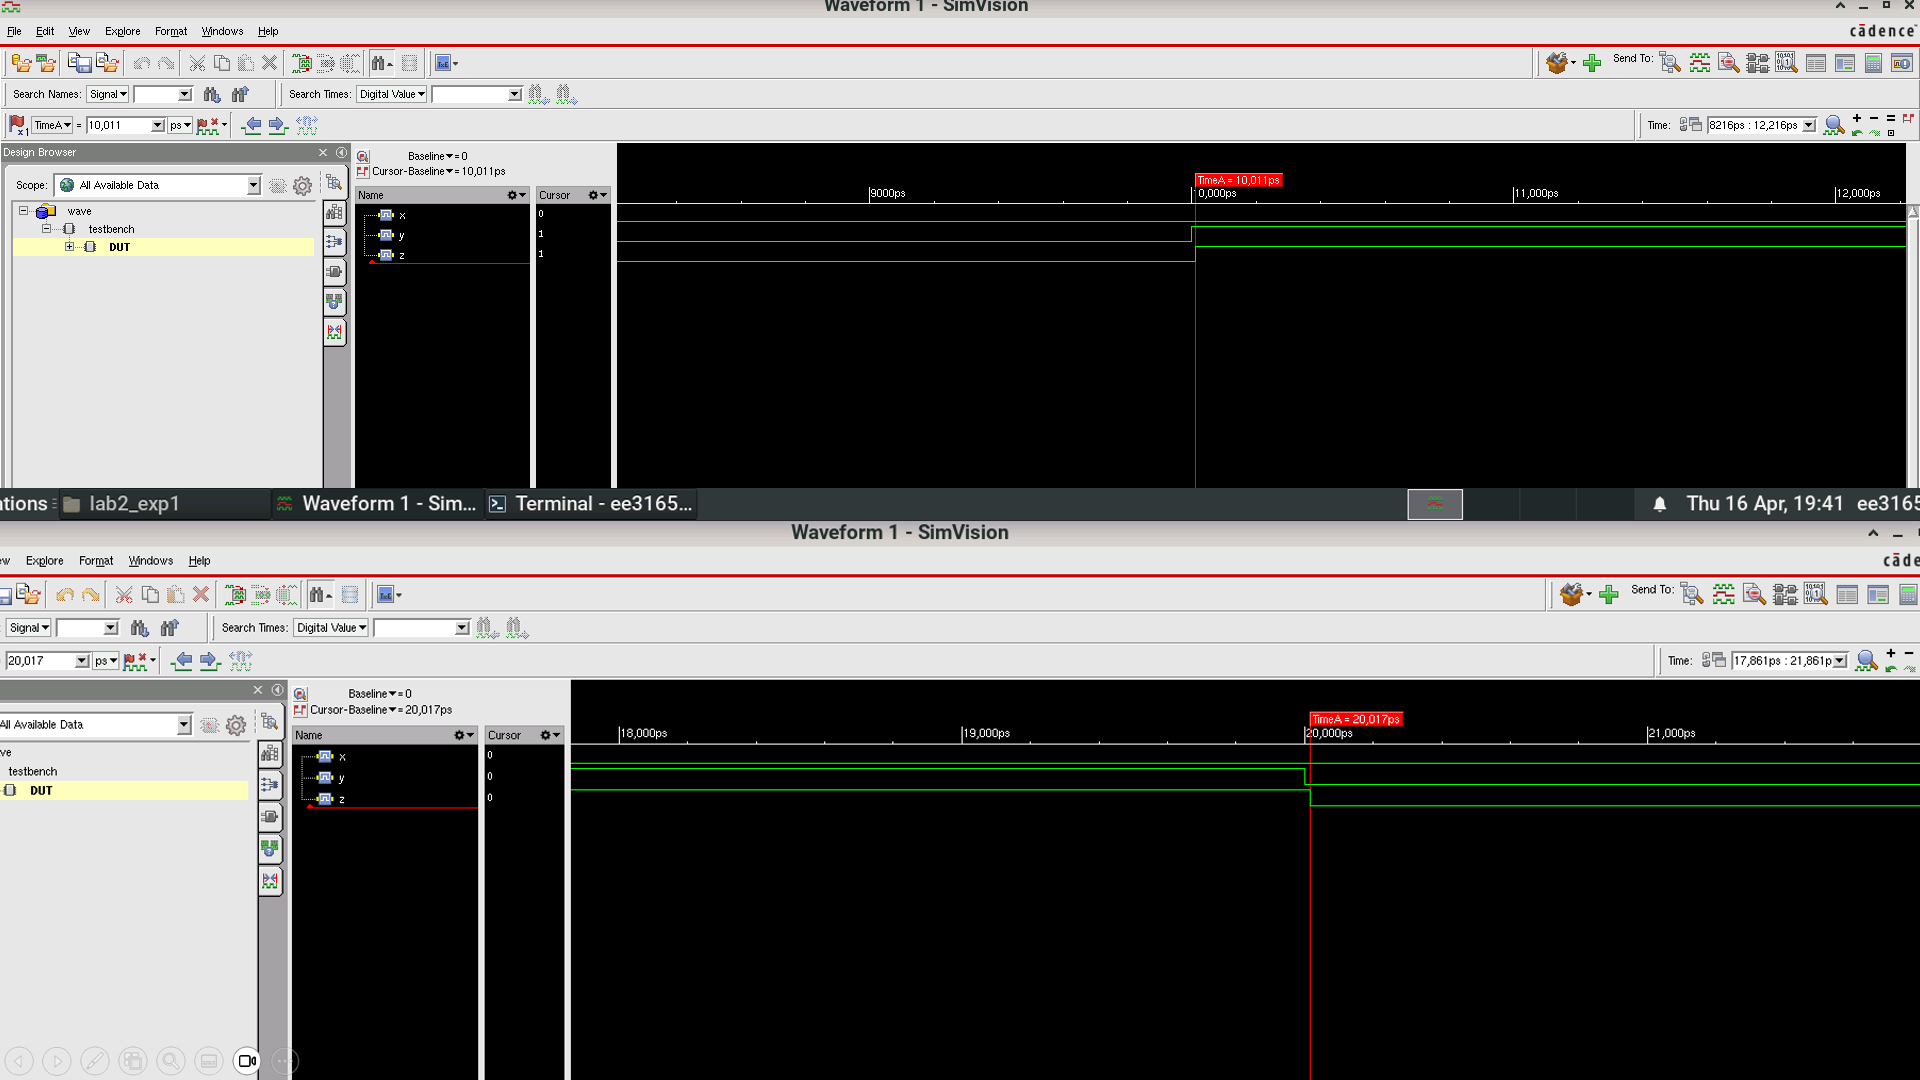
\includegraphics[width=\textwidth]{figures/exp1_or2_lvt_fast_1v0.png}
        \caption{Corner LVT Fast (fast\_vdd1v0)}
        \label{fig:or2_lvt_fast_1v0}
    \end{subfigure}
    \hfill
    % --- Hình bên phải: LVT Slow ---
    \begin{subfigure}[b]{0.48\textwidth}
        \centering
        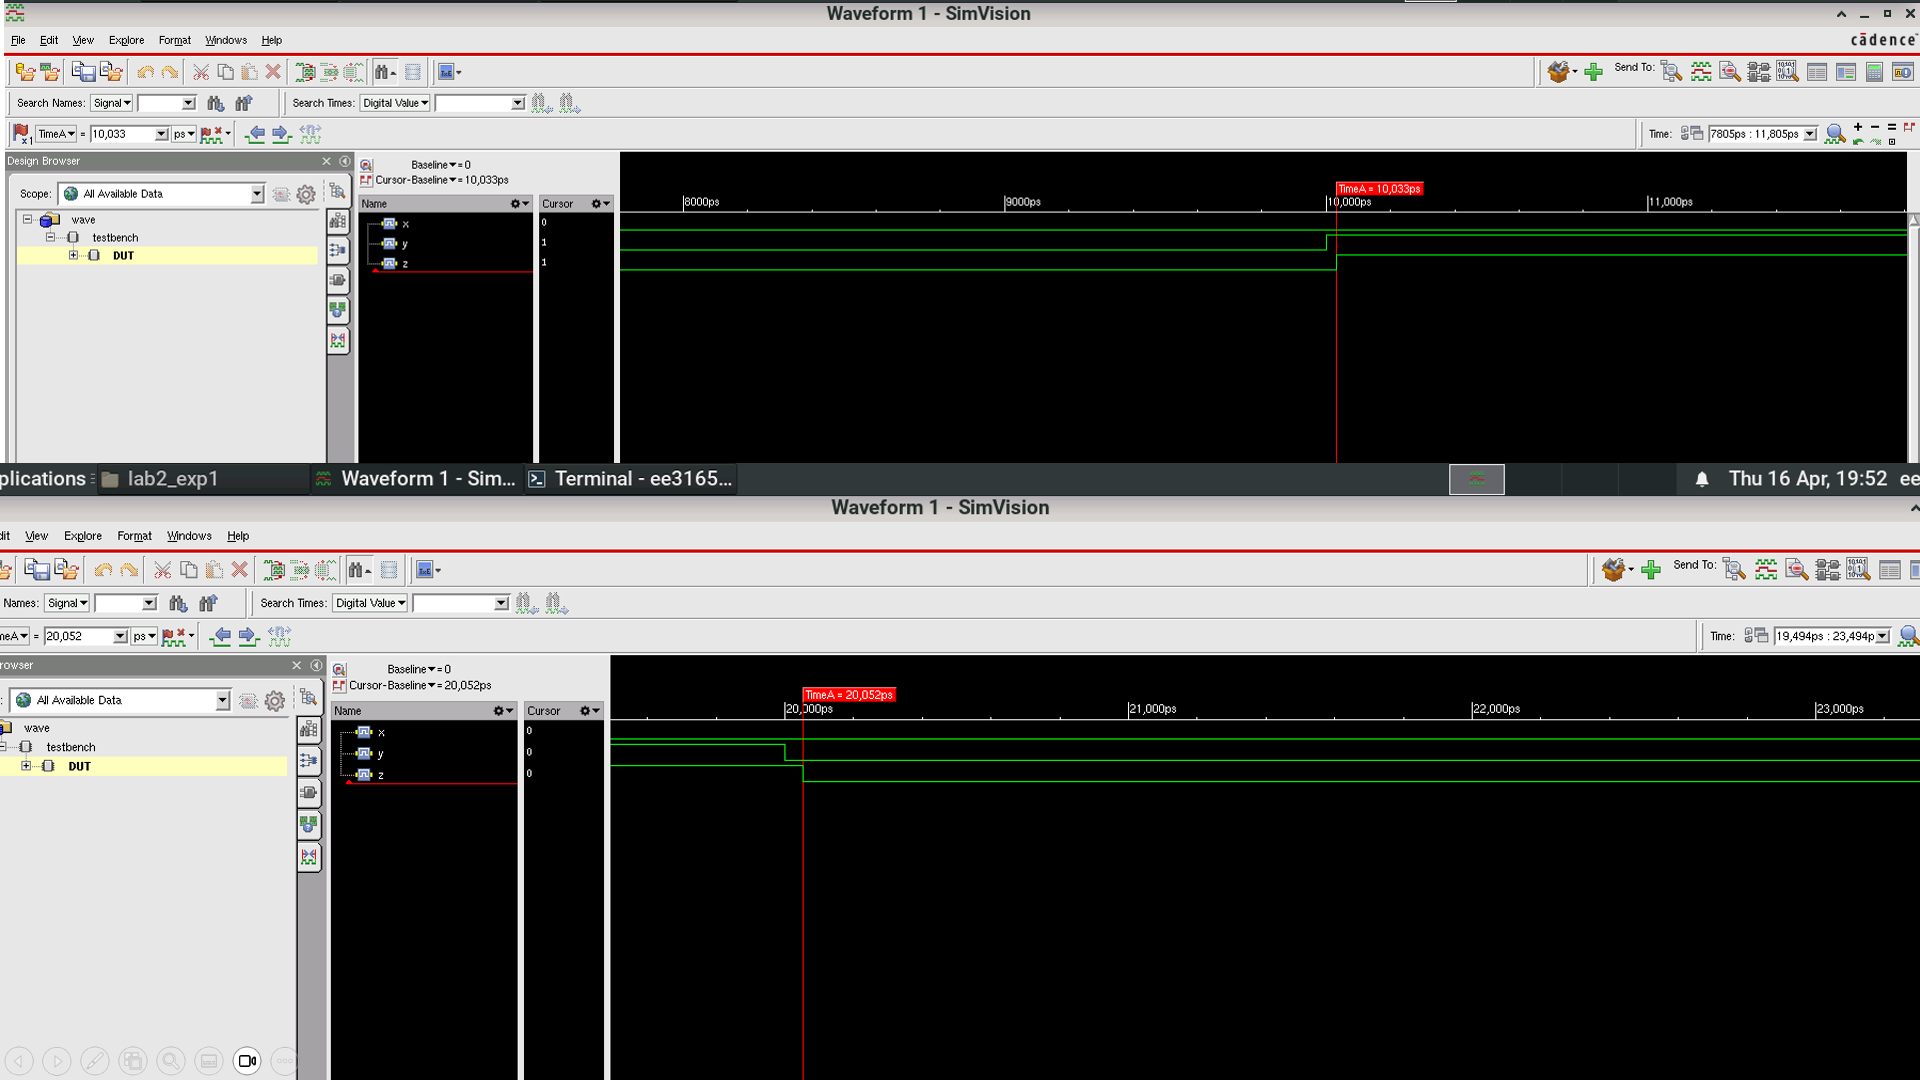
\includegraphics[width=\textwidth]{figures/exp1_or2_lvt_slow_1v0.png}
        \caption{Corner LVT Slow (slow\_vdd1v0)}
        \label{fig:or2_lvt_slow_1v0}
    \end{subfigure}
    
    \caption{Waveform đo độ trễ cổng OR2 sử dụng thư viện LVT ở 1.0V. Quan sát thấy độ trễ được cải thiện đáng kể so với thư viện HVT ở cùng điều kiện vận hành.}
    \label{fig:or2_lvt_comparison_1v0}
\end{figure}

\textbf{Nhận xét (LVT - 1.0V):} Khi hoạt động ở trạng thái thiếu điện áp (1.0V), mạch LVT chứng tỏ được giá trị của mình:
\begin{itemize}
    \item \textbf{Duy trì tốc độ ở điện áp thấp:} So chiếu với góc \texttt{slow\_vdd1v0} của HVT ($0.099ns$), cổng OR2 LVT chỉ mất $0.052ns$ để chuyển mạch sườn xuống, cải thiện gần $50\%$ tốc độ. Điều này biến LVT thành "cứu cánh" tuyệt vời cho các đường dẫn tới hạn trong thiết kế Low Power.
    \item \textbf{Đánh đổi năng lượng rò:} Nhược điểm là ở góc Slow, LVT tiêu hao $1.26 \times 10^{-8}W$, cao hơn mức $1.15 \times 10^{-8}W$ của HVT do dòng rò dưới ngưỡng luôn lớn.
\end{itemize}

Mô phỏng tại góc điện áp 1.2V cho thư viện LVT nhằm xác định giới hạn tốc độ tối đa của linh kiện.

\begin{figure}[H]
    \centering
    % --- Hình bên trái: LVT Fast ---
    \begin{subfigure}[b]{0.48\textwidth}
        \centering
        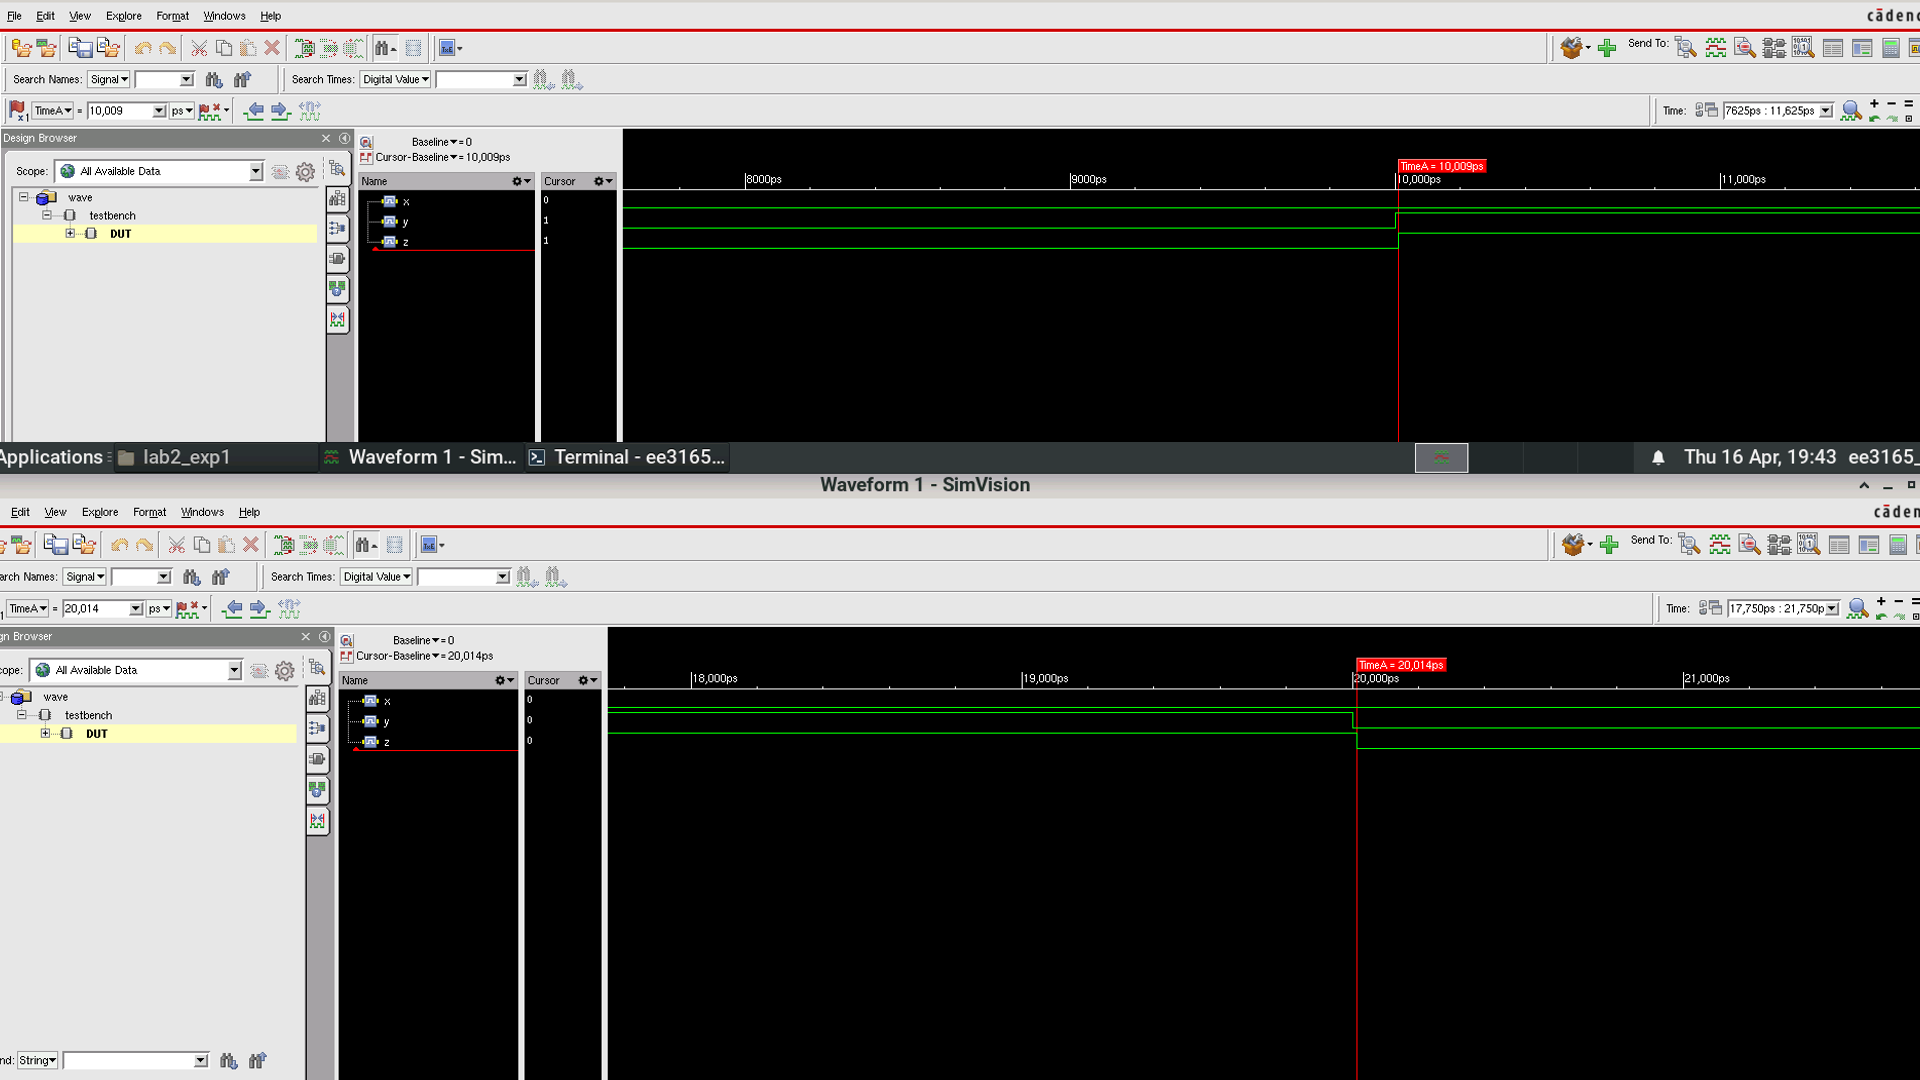
\includegraphics[width=\textwidth]{figures/exp1_or2_lvt_fast_1v2.png}
        \caption{Corner LVT Fast (fast\_vdd1v2)}
        \label{fig:or2_lvt_fast_1v2}
    \end{subfigure}
    \hfill
    % --- Hình bên phải: LVT Slow ---
    \begin{subfigure}[b]{0.48\textwidth}
        \centering
        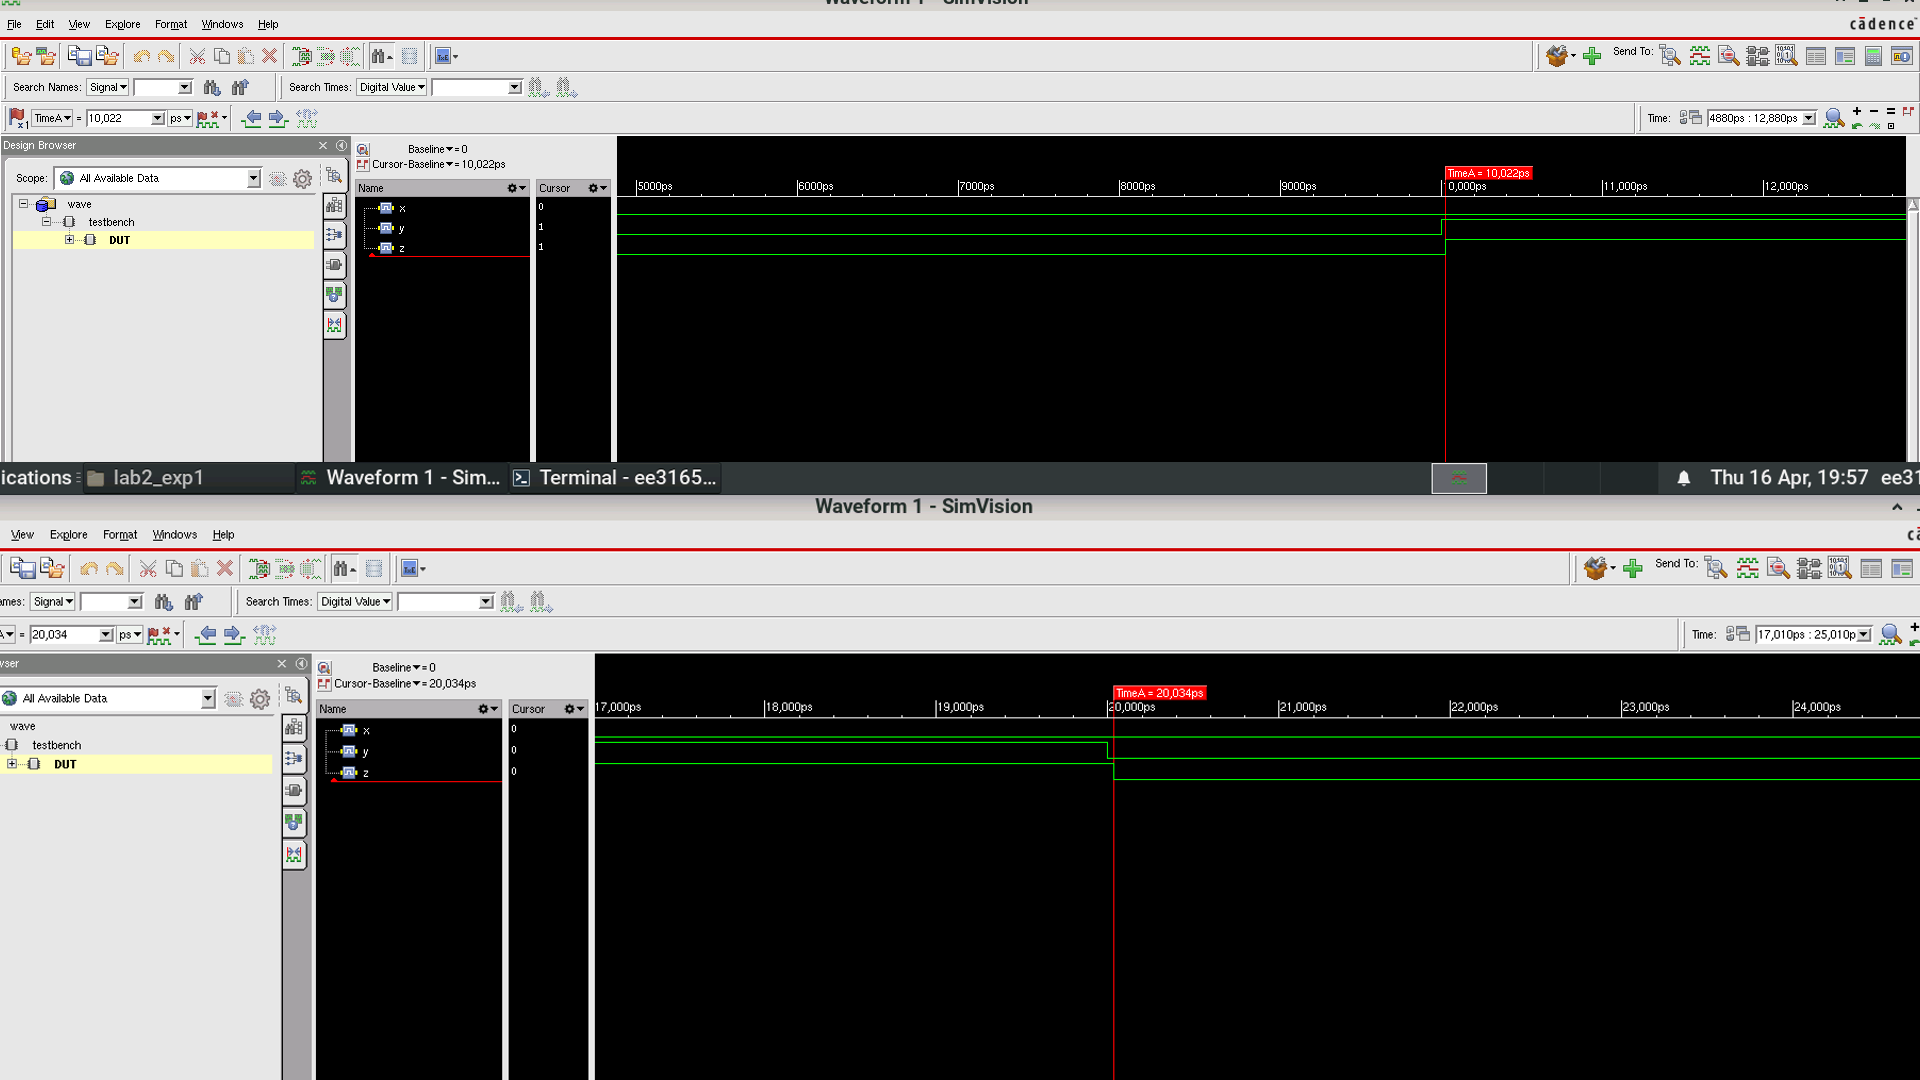
\includegraphics[width=\textwidth]{figures/exp1_or2_lvt_slow_1v2.png}
        \caption{Corner LVT Slow (slow\_vdd1v2)}
        \label{fig:or2_lvt_slow_1v2}
    \end{subfigure}
    
    \caption{Waveform đo độ trễ cổng OR2 sử dụng thư viện LVT với VDD=1.2V}
    \label{fig:or2_lvt_comparison_1v2}
\end{figure}

\textbf{Nhận xét (LVT - 1.2V):}
\begin{itemize}
    \item \textbf{Tốc độ cực hạn:} Tại góc \texttt{fast\_vdd1v2\_lvt}, cổng OR2 đạt ngưỡng hiệu năng tối đa. Rising Delay của chân B chạm đáy ở mức $0.008ns$, sườn xung vô cùng dốc, đáp ứng tốt cho các hệ thống xung nhịp Gigahertz.
    \item \textbf{Nguy cơ về nhiệt:} Tại góc này, công suất tĩnh và động cộng hưởng đẩy mức tiêu hao lên đỉnh điểm $3.34 \times 10^{-8}W$. Do đó, bộ tổng hợp chỉ nên chèn cell này một cách cực kỳ chọn lọc để tránh vi phạm giới hạn nhiệt.
\end{itemize}

\paragraph{C. Kết luận} 

Từ việc phân tích chéo số liệu thực tế, nhóm rút ra các quy luật PPA mang tính cốt lõi cho kỹ sư thiết kế vật lý:
\begin{itemize}
    \item \textbf{Tính bất biến của diện tích:} Xuyên suốt 8 góc mô phỏng, Area luôn giữ cố định ở mức $1.368 \mu m^2$, khẳng định kích thước vật lý của Standard Cell là độc lập với điều kiện vận hành.
    \item \textbf{Bài toán đánh đổi:} LVT ép xung xuất sắc (giảm trễ từ $0.099ns$ xuống $0.008ns$) nhưng yêu cầu trả giá đắt về rò rỉ điện năng (tăng từ $\sim 11.4nW$ lên $\sim 33.4nW$). Giải pháp Multi-Vth tối ưu trong thực tế là dùng \textbf{HVT làm nòng cốt} để tiết kiệm pin và chỉ điểm xuyết \textbf{LVT ở các đường dẫn vi phạm Timing}.
\end{itemize}

\newpage
\subsubsection{NAND2}
\begin{lstlisting}[style={prettyverilog}, caption={\texttt{code thiết kế cổng NAND}}]
`timescale 1ns/1ps
module nand(
    input logic A,
    input logic B,
      output logic Y);
    assign Y = A & B;
endmodule
\end{lstlisting}
\begin{lstlisting}[style={prettyverilog}, caption={\texttt{code testbench cổng NAND}}]
`timescale 1ns/1ps
module tb_nand;
    logic A, B;
    logic Y;
    nand(.A(A), .B(B), .Y(Y));
    initial begin
        $dumpfile("nand_wave.vcd");
        $dumpvars(0, tb_nand);
        A = 0; B = 0; #10;
        A = 0; B = 1; #10;
        A = 1; B = 0; #10;
        A = 1; B = 1; #10;
        $finish;
    end
endmodule
\end{lstlisting}

Trước hết, để tổng quan về linh kiện, Hình \ref{fig:exp1_nand2} trình bày ký hiệu logic cơ bản của cổng NAND2. Linh kiện này thực hiện hàm logic đảo của cổng AND, với phương trình đại số Boole $Y = \overline{A \cdot B}$ (ngõ ra chỉ ở mức 0 khi cả hai ngõ vào đồng thời ở mức 1).

\begin{figure}[H]
    \centering
    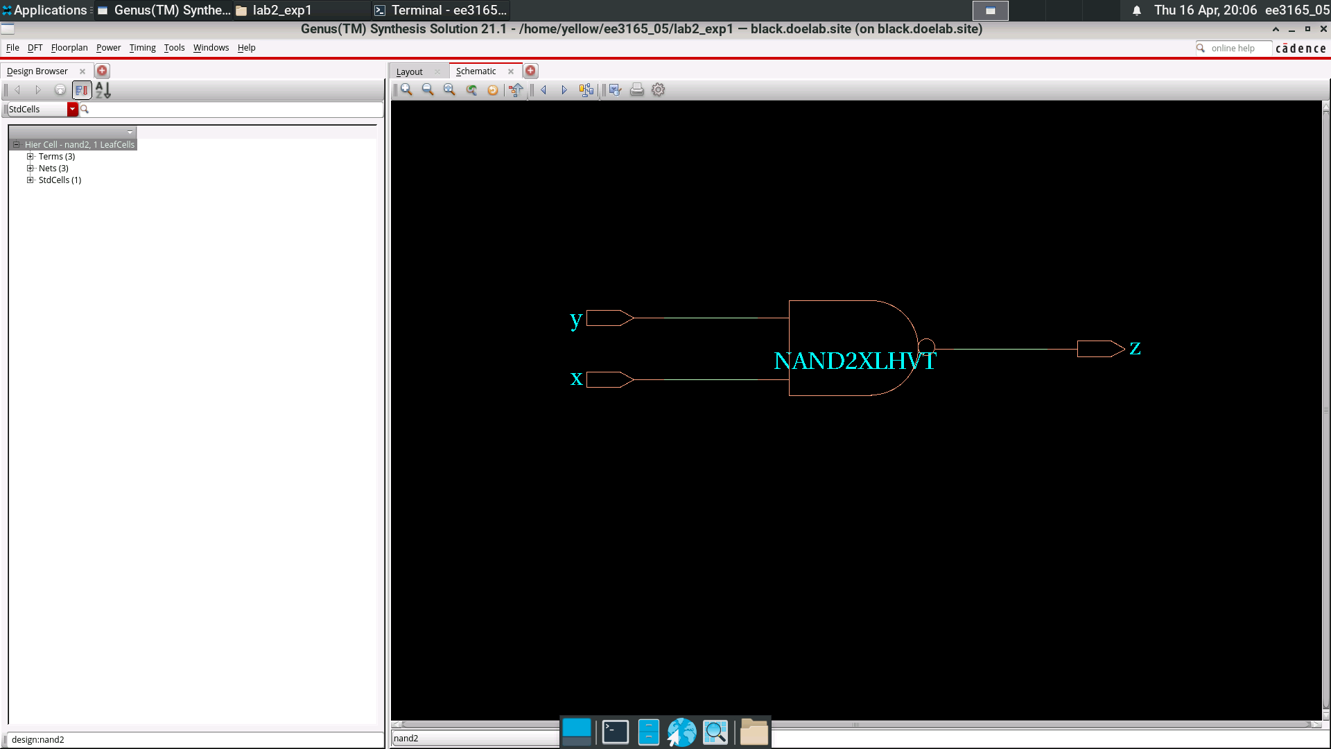
\includegraphics[width=0.6\textwidth]{figures/exp1_nand2.png}
    \caption{Ký hiệu schematic và đặc tính logic cơ bản của cổng NAND2.}
    \label{fig:exp1_nand2}
\end{figure}

Sau khi viết mã RTL, thiết kế được đưa vào công cụ Genus để thực hiện quá trình tổng hợp. Hình \ref{fig:exp1_nand2_mapped} minh họa sơ đồ mức cổng của cổng NAND2 sau khi được ánh xạ vào thư viện công nghệ 45nm.

\begin{figure}[H]
    \centering
    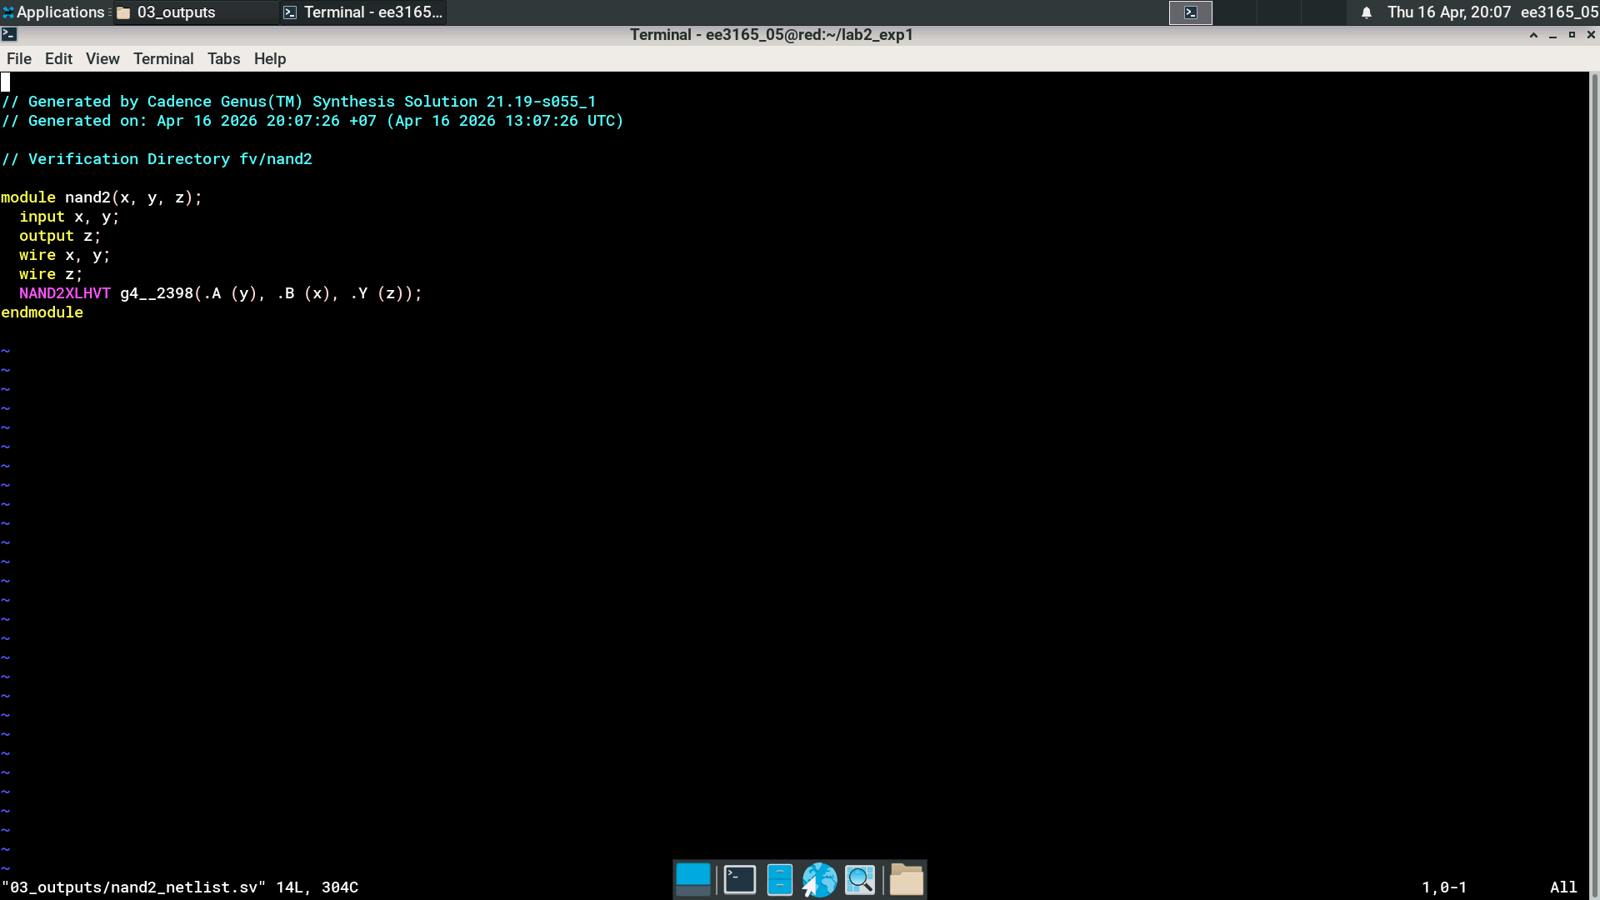
\includegraphics[width=0.7\textwidth]{figures/exp1_nand2_mapped.png}
    \caption{Sơ đồ mức cổng của thiết kế NAND2 trên giao diện Genus.}
    \label{fig:exp1_nand2_mapped}
\end{figure}

Nhóm tiếp tục thực hiện khảo sát đặc tính của cổng NAND2 trên cả hai loại thư viện: High Threshold Voltage (HVT) và Low Threshold Voltage (LVT).

\paragraph{A. Thư viện High Threshold Voltage (HVT)}
Đặc tính của các cell HVT là dòng rò thấp nhưng độ trễ lớn hơn. Kết quả mô phỏng 8 corners được tổng hợp trong bảng dưới đây:

\begin{table}[H]
\centering
\renewcommand{\arraystretch}{1.3}
\resizebox{\textwidth}{!}{
\begin{tabular}{|l|c|c|c|c|c|c|}
\hline
 
\multirow{2}{*}{\textbf{Library Name}} 
& \multirow{2}{*}{\textbf{Total Area}} 
& \multirow{2}{*}{\textbf{Total Power}} 
 
& \multicolumn{2}{c|}{\textbf{Delay Parameter A$\rightarrow$Y}}
& \multicolumn{2}{c|}{\textbf{Delay Parameter B$\rightarrow$Y}} \\
 
\cline{4-7}
 
& & 
& \textbf{Rising Delay (ns)} 
& \textbf{Falling Delay (ns)}
& \textbf{Rising Delay (ns)} 
& \textbf{Falling Delay (ns)} \\
 
\hline
 
% ----------- KHỐI HVT ----------------
 
fast\_vdd1v0\_basicCells\_hvt 
& 1.026 & 1.05962e-08 
& 0.007 & 0.011
& 0.005 & 0.008 \\ \hline
 
fast\_vdd1v2\_basicCells\_hvt 
& 1.026 & 1.54143e-08 
& 0.006 & 0.008
& 0.004 & 0.006 \\ \hline
 
slow\_vdd1v0\_basicCells\_hvt 
& 1.026 & 7.20719e-09 
& 0.017 & 0.066
& 0.012 & 0.050 \\ \hline
 
slow\_vdd1v2\_basicCells\_hvt 
& 1.026 & 1.04670e-08 
& 0.010 & 0.029
& 0.007 & 0.021 \\ \hline
 
\end{tabular}
}

\caption{Tổng hợp thông số Diện tích, Công suất và Độ trễ của cổng NAND2 (HVT).}
\label{tab:exp1_nand2_hvt_params}

\end{table}

Dưới đây là sự so sánh dạng sóng mô phỏng của cổng NAND2 tại hai góc cực đoan: Fast (nhanh nhất) và Slow (chậm nhất) ở cùng mức điện áp 1.0V.

\begin{figure}[H]
    \centering
    \begin{subfigure}[b]{0.48\textwidth}
        \centering
        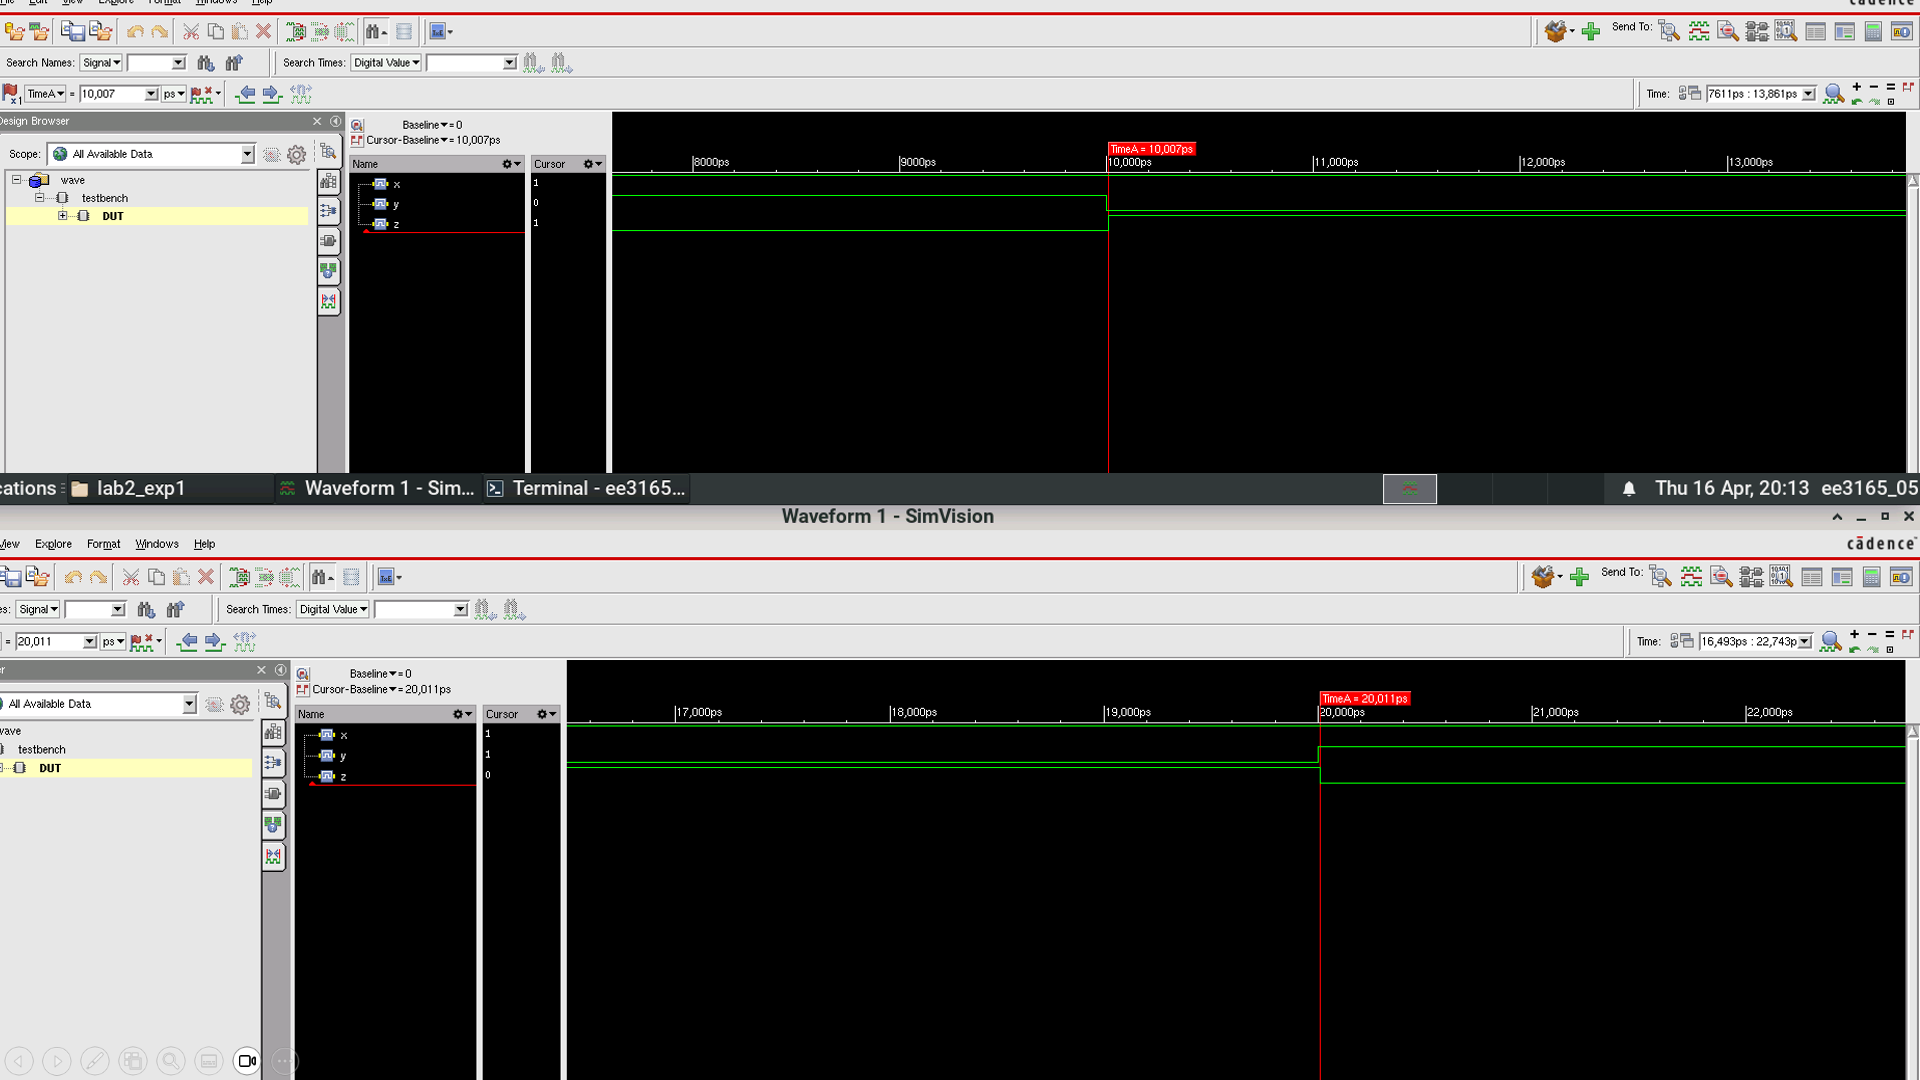
\includegraphics[width=\textwidth]{figures/exp1_nand2_hvt_fast_1v0.png}
        \caption{Corner HVT Fast (fast\_vdd1v0)}
    \end{subfigure}
    \hfill
    \begin{subfigure}[b]{0.48\textwidth}
        \centering
        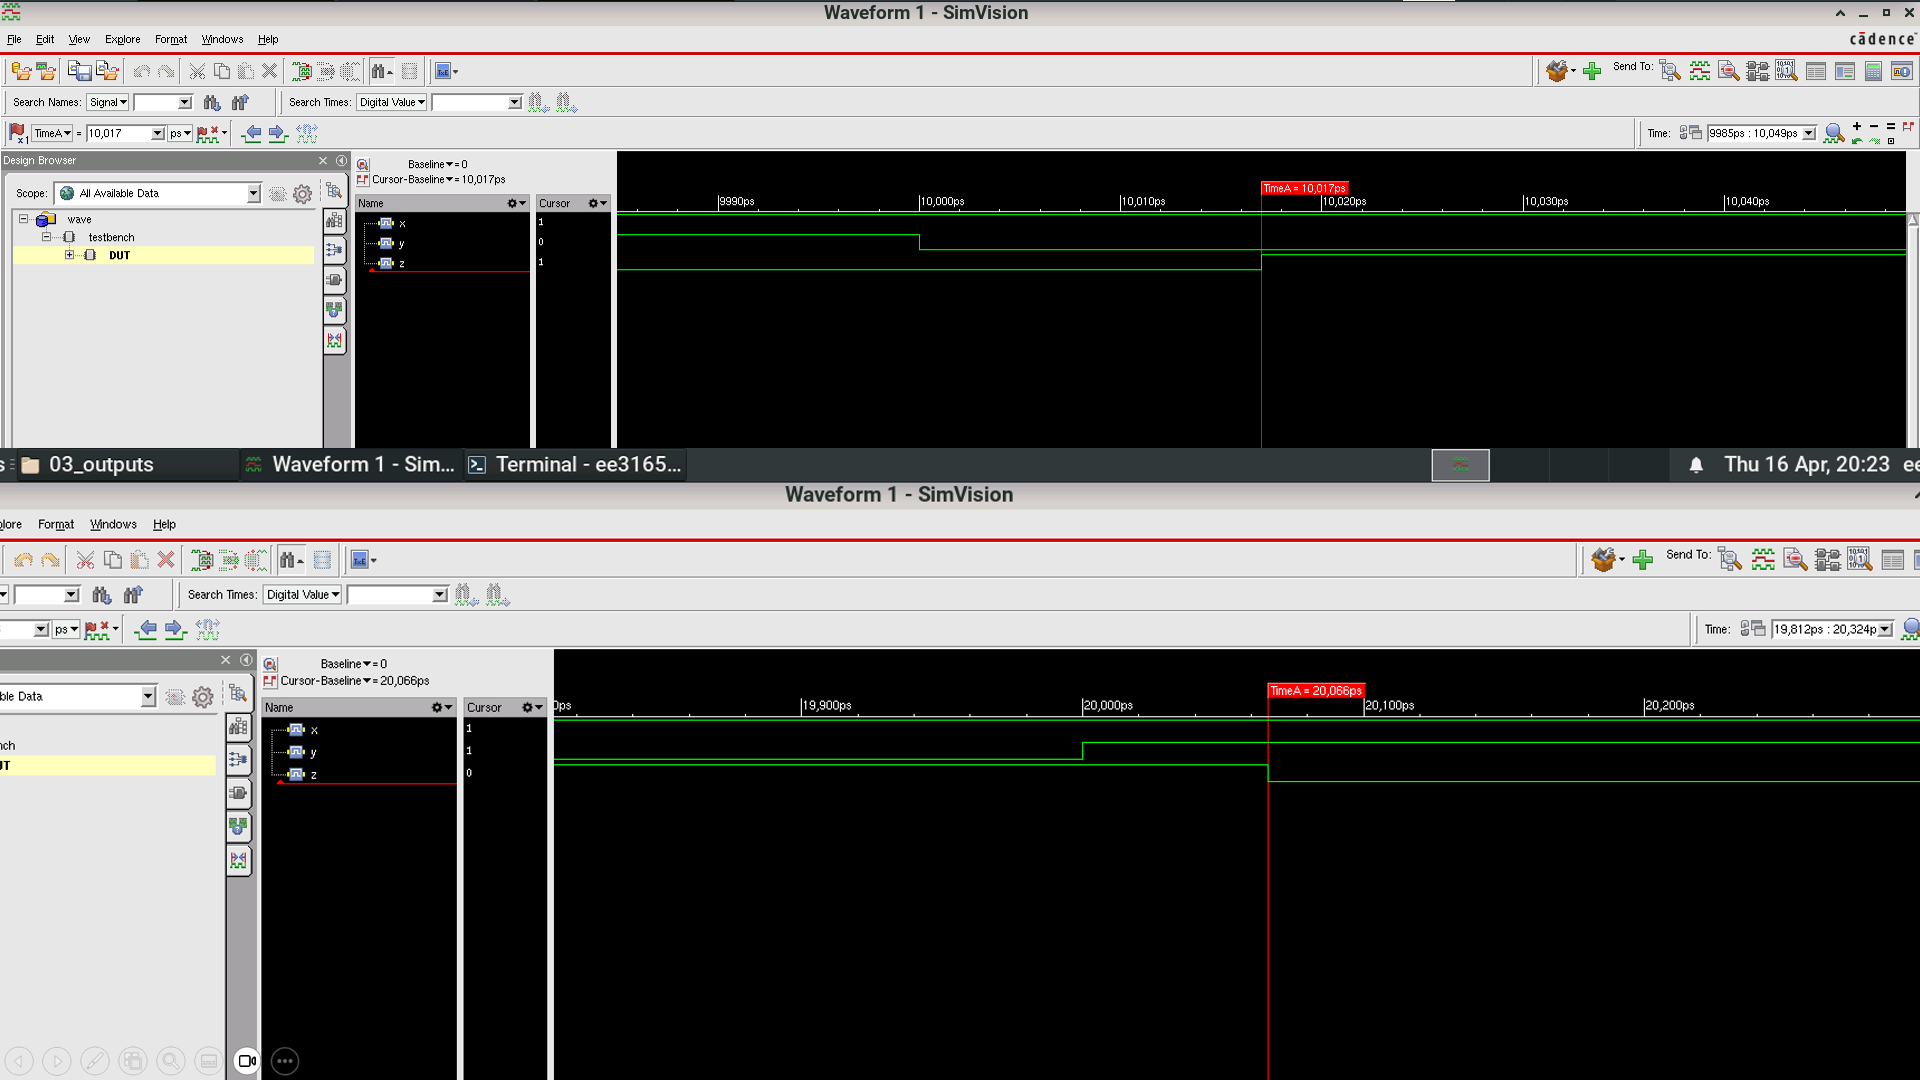
\includegraphics[width=\textwidth]{figures/exp1_nand2_hvt_slow_1v0.png}
        \caption{Corner HVT Slow (slow\_vdd1v0)}
    \end{subfigure}
    \caption{So sánh Waveform đo độ trễ cổng NAND2 ở HVT (VDD = 1.0V).}
    \label{fig:nand2_hvt_comparison_1v0}
\end{figure}

\textbf{Nhận xét (HVT - 1.0V):} Dựa trên số liệu đo đạc tại mức điện áp 1.0V, ta có thể thấy rõ đặc trưng kiến trúc của cổng NAND2:
\begin{itemize}
    \item \textbf{Điểm nghẽn sườn xuống:} Trái ngược với cổng NOR, cổng NAND2 có hai transistor NMOS mắc nối tiếp ở mạng kéo xuống. Điều này làm tăng điện trở tương đương, khiến thời gian xả tụ kéo dài. Bảng số liệu cho thấy độ trễ sườn xuống luôn lớn hơn sườn lên đáng kể. Đặc biệt tại góc chậm nhất \texttt{slow\_vdd1v0\_hvt}, độ trễ sườn xuống của chân A chạm mức $0.066ns$, trong khi sườn lên chỉ mất $0.017ns$.
    \item \textbf{Đặc tính bất đối xứng:} Tương tự các cổng nhiều ngõ vào khác, độ trễ từ chân A luôn lớn hơn chân B (ví dụ $0.066ns$ so với $0.050ns$). Sự chênh lệch này xuất phát từ vị trí vật lý của transistor trên mạch tích hợp.
    \item \textbf{Tối ưu hóa năng lượng tĩnh:} Ở điều kiện điện áp thấp và góc chậm nhất, cổng NAND2 thể hiện khả năng tiết kiệm điện xuất sắc với mức tiêu thụ chỉ $7.207 \times 10^{-9}W$.
\end{itemize}

\vspace{1cm}

Dưới đây là kết quả mô phỏng tại điện áp danh định 1.2V cho thư viện HVT.

\begin{figure}[H]
    \centering
    \begin{subfigure}[b]{0.48\textwidth}
        \centering
        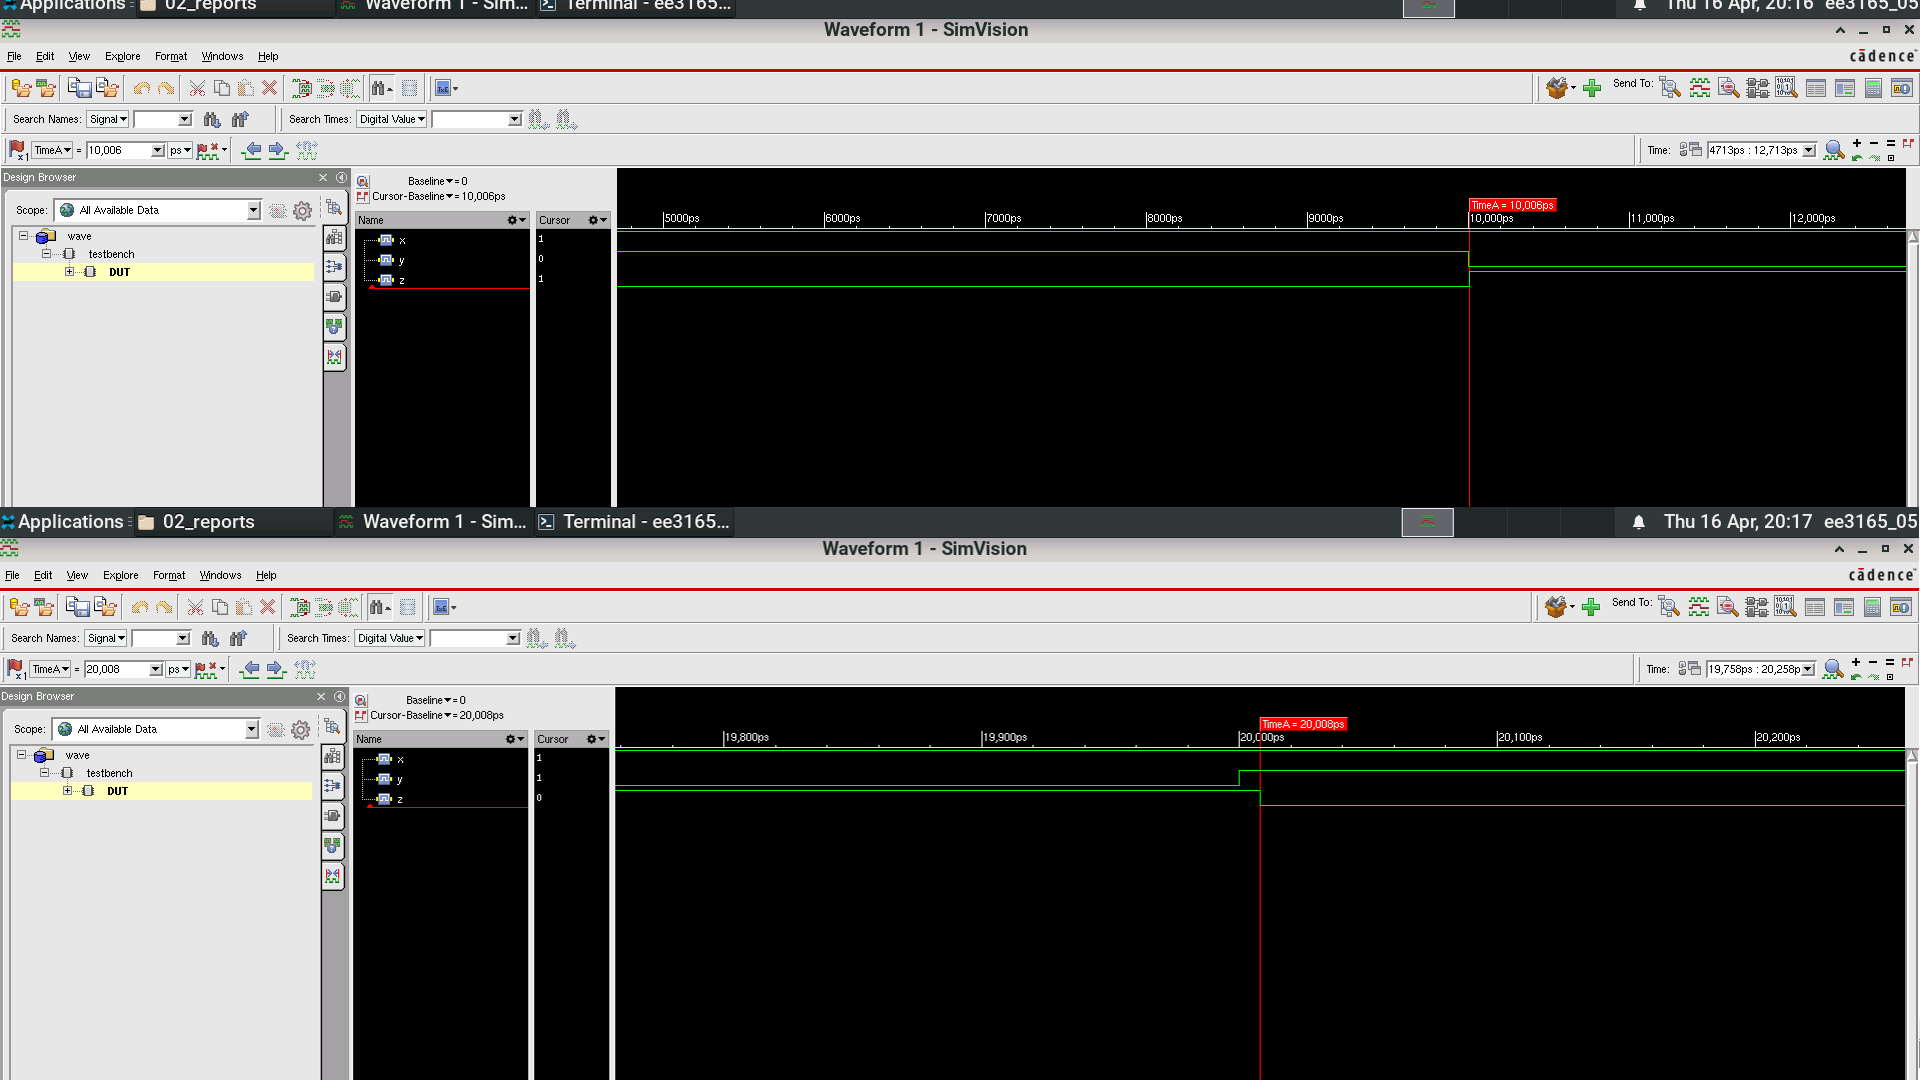
\includegraphics[width=\textwidth]{figures/exp1_nand2_hvt_fast_1v2.png}
        \caption{Corner HVT Fast (fast\_vdd1v2)}
    \end{subfigure}
    \hfill
    \begin{subfigure}[b]{0.48\textwidth}
        \centering
        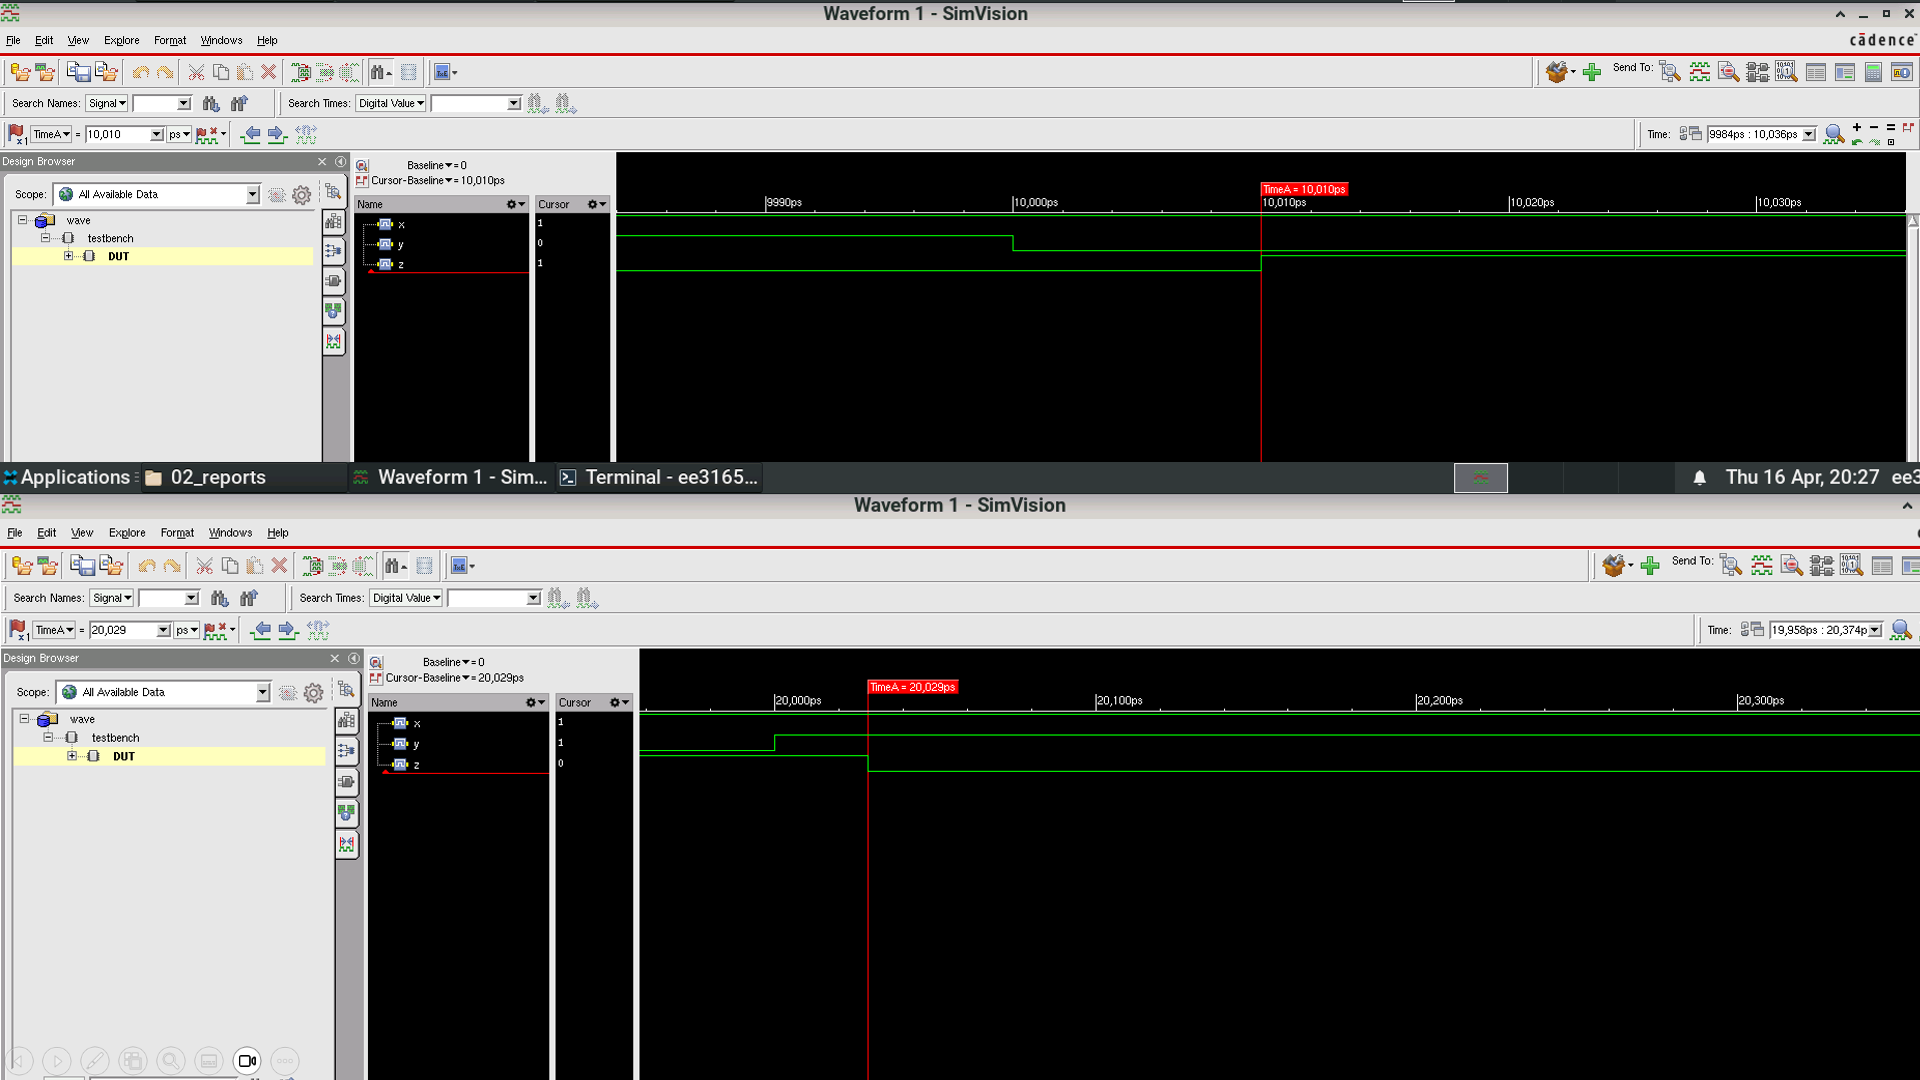
\includegraphics[width=\textwidth]{figures/exp1_nand2_hvt_slow_1v2.png}
        \caption{Corner HVT Slow (slow\_vdd1v2)}
    \end{subfigure}
    \caption{So sánh Waveform đo độ trễ cổng NAND2 ở HVT (VDD = 1.2V).}
    \label{fig:nand2_hvt_comparison_1v2}
\end{figure}

\textbf{Nhận xét (HVT - 1.2V):} Khi cung cấp đủ mức điện áp danh định 1.2V:
\begin{itemize}
    \item \textbf{Khắc phục hiện tượng đói dòng:} Dòng điện bão hòa tăng mạnh giúp cải thiện rõ rệt thời gian nạp xả tụ. Ở góc nhanh nhất, độ trễ sườn lên ngõ B giảm xuống chỉ còn $0.004ns$. Độ trễ sườn xuống cũng được cải thiện mạnh mẽ.
    \item \textbf{Gia tăng công suất động:} Việc tăng điện áp khiến công suất tiêu thụ vọt lên mức $1.54 \times 10^{-8}W$ ở góc nhanh nhất, tuân đúng theo tỷ lệ bình phương của điện áp nguồn.
\end{itemize}

\paragraph{B. Thư viện Low Threshold Voltage (LVT)}
Các cell LVT cho tốc độ chuyển mạch nhanh hơn nhờ điện áp ngưỡng thấp, đổi lại công suất tiêu thụ tĩnh cao hơn.

\begin{table}[H]
\centering
\renewcommand{\arraystretch}{1.3}
\resizebox{\textwidth}{!}{
\begin{tabular}{|l|c|c|c|c|c|c|}
\hline
 
\multirow{2}{*}{\textbf{Library Name}} 
& \multirow{2}{*}{\textbf{Total Area}} 
& \multirow{2}{*}{\textbf{Total Power}} 
 
& \multicolumn{2}{c|}{\textbf{Delay Parameter A$\rightarrow$Y}}
& \multicolumn{2}{c|}{\textbf{Delay Parameter B$\rightarrow$Y}} \\
 
\cline{4-7}
 
& & 
& \textbf{Rising Delay (ns)} 
& \textbf{Falling Delay (ns)}
& \textbf{Rising Delay (ns)} 
& \textbf{Falling Delay (ns)} \\
 
\hline
 
% ----------- KHỐI LVT ----------------
 
fast\_vdd1v0\_basicCells\_lvt 
& 1.026 & 1.42490e-08 
& 0.005 & 0.006
& 0.004 & 0.005 \\ \hline
 
fast\_vdd1v2\_basicCells\_lvt 
& 1.026 & 2.00986e-08 
& 0.004 & 0.005
& 0.003 & 0.004 \\ \hline
 
slow\_vdd1v0\_basicCells\_lvt 
& 1.026 & 7.73734e-09 
& 0.010 & 0.024
& 0.007 & 0.018 \\ \hline
 
slow\_vdd1v2\_basicCells\_lvt 
& 1.026 & 1.11834e-08 
& 0.008 & 0.015
& 0.006 & 0.012 \\ \hline
 
\end{tabular}
}
 
\caption{Tổng hợp thông số Diện tích, Công suất và Độ trễ của NAND2 (LVT).}
\label{tab:exp1_nand2_lvt_params}

\end{table}

\textbf{Khảo sát đặc tính LVT tại điều kiện 1.0V (Điện áp thấp):}

Dưới đây là kết quả mô phỏng dạng sóng của cổng NAND2 LVT tại mức điện áp 1.0V để đánh giá khả năng duy trì hiệu suất khi hạ nguồn.

\begin{figure}[H]
    \centering
    \begin{subfigure}[b]{0.48\textwidth}
        \centering
        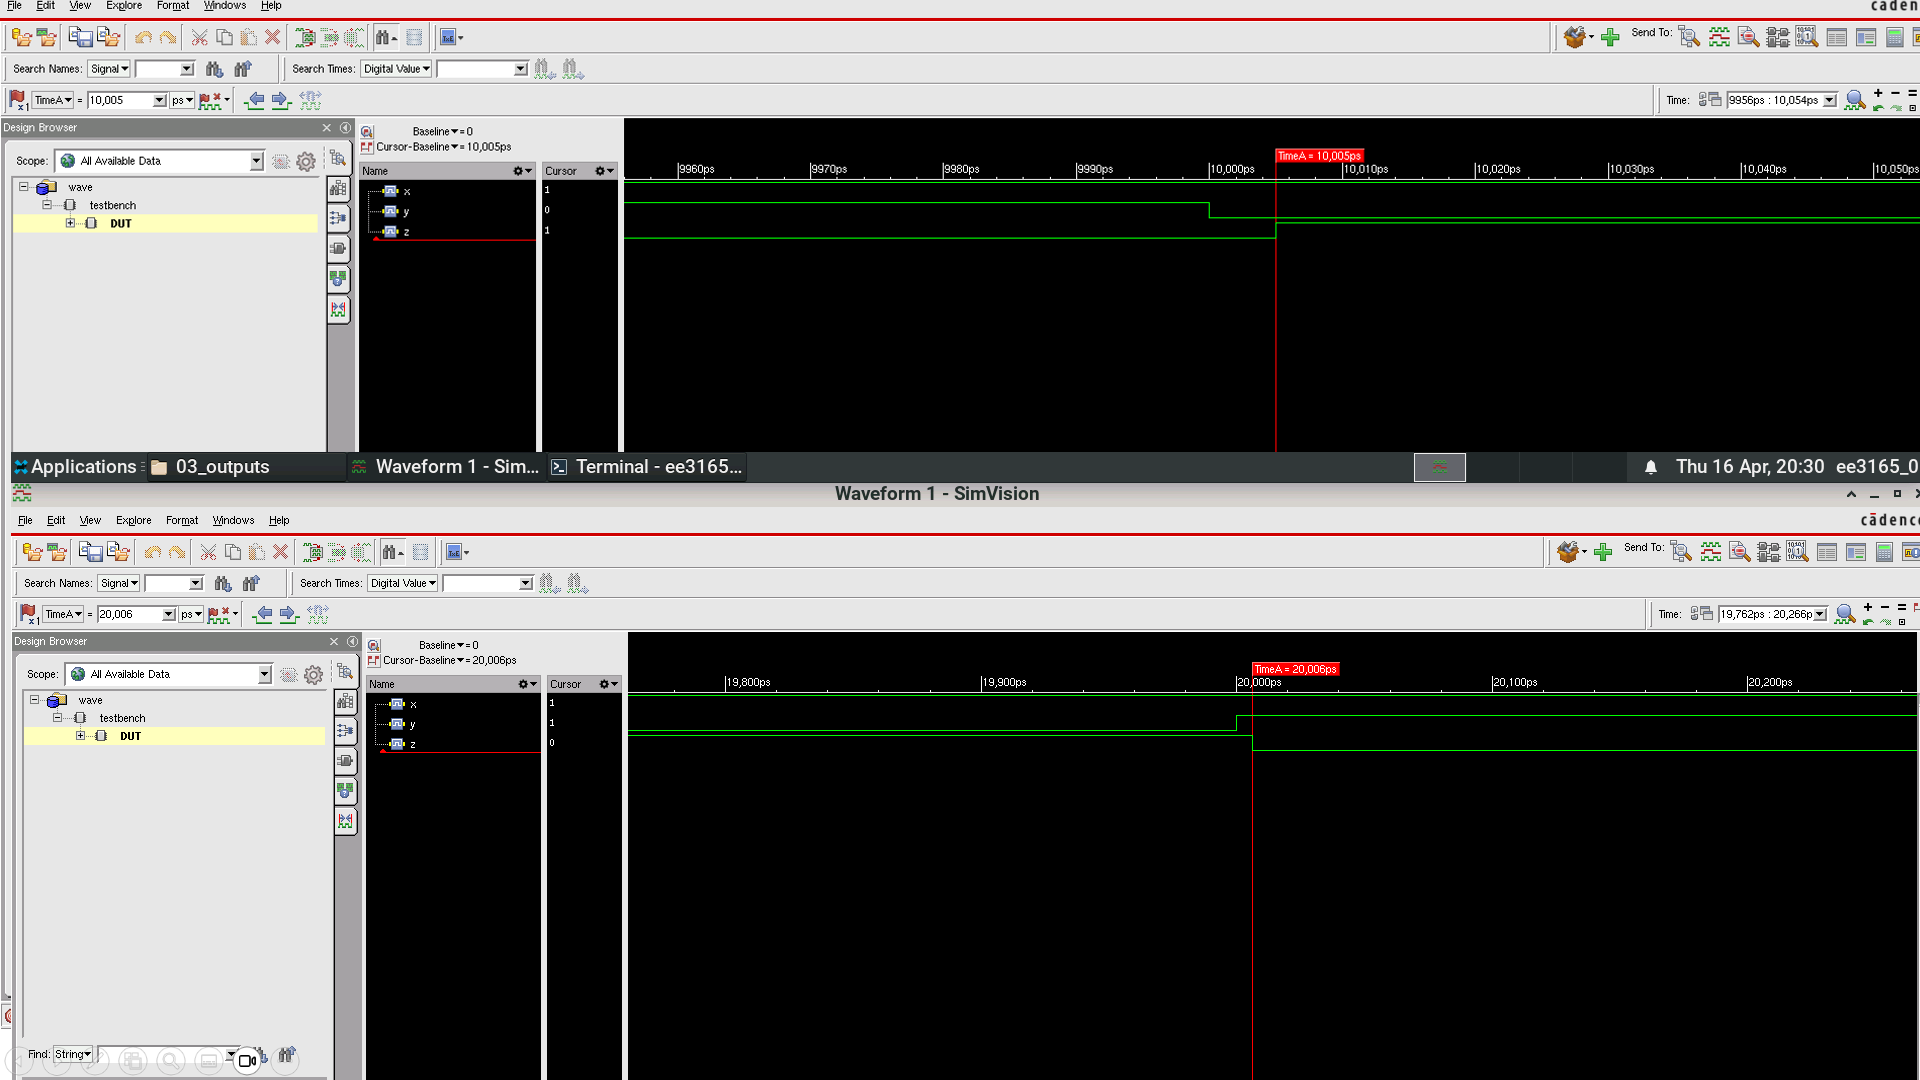
\includegraphics[width=\textwidth]{figures/exp1_nand2_lvt_fast_1v0.png}
        \caption{Corner LVT Fast (fast\_vdd1v0)}
        \label{fig:nand2_lvt_fast_1v0}
    \end{subfigure}
    \hfill
    \begin{subfigure}[b]{0.48\textwidth}
        \centering
        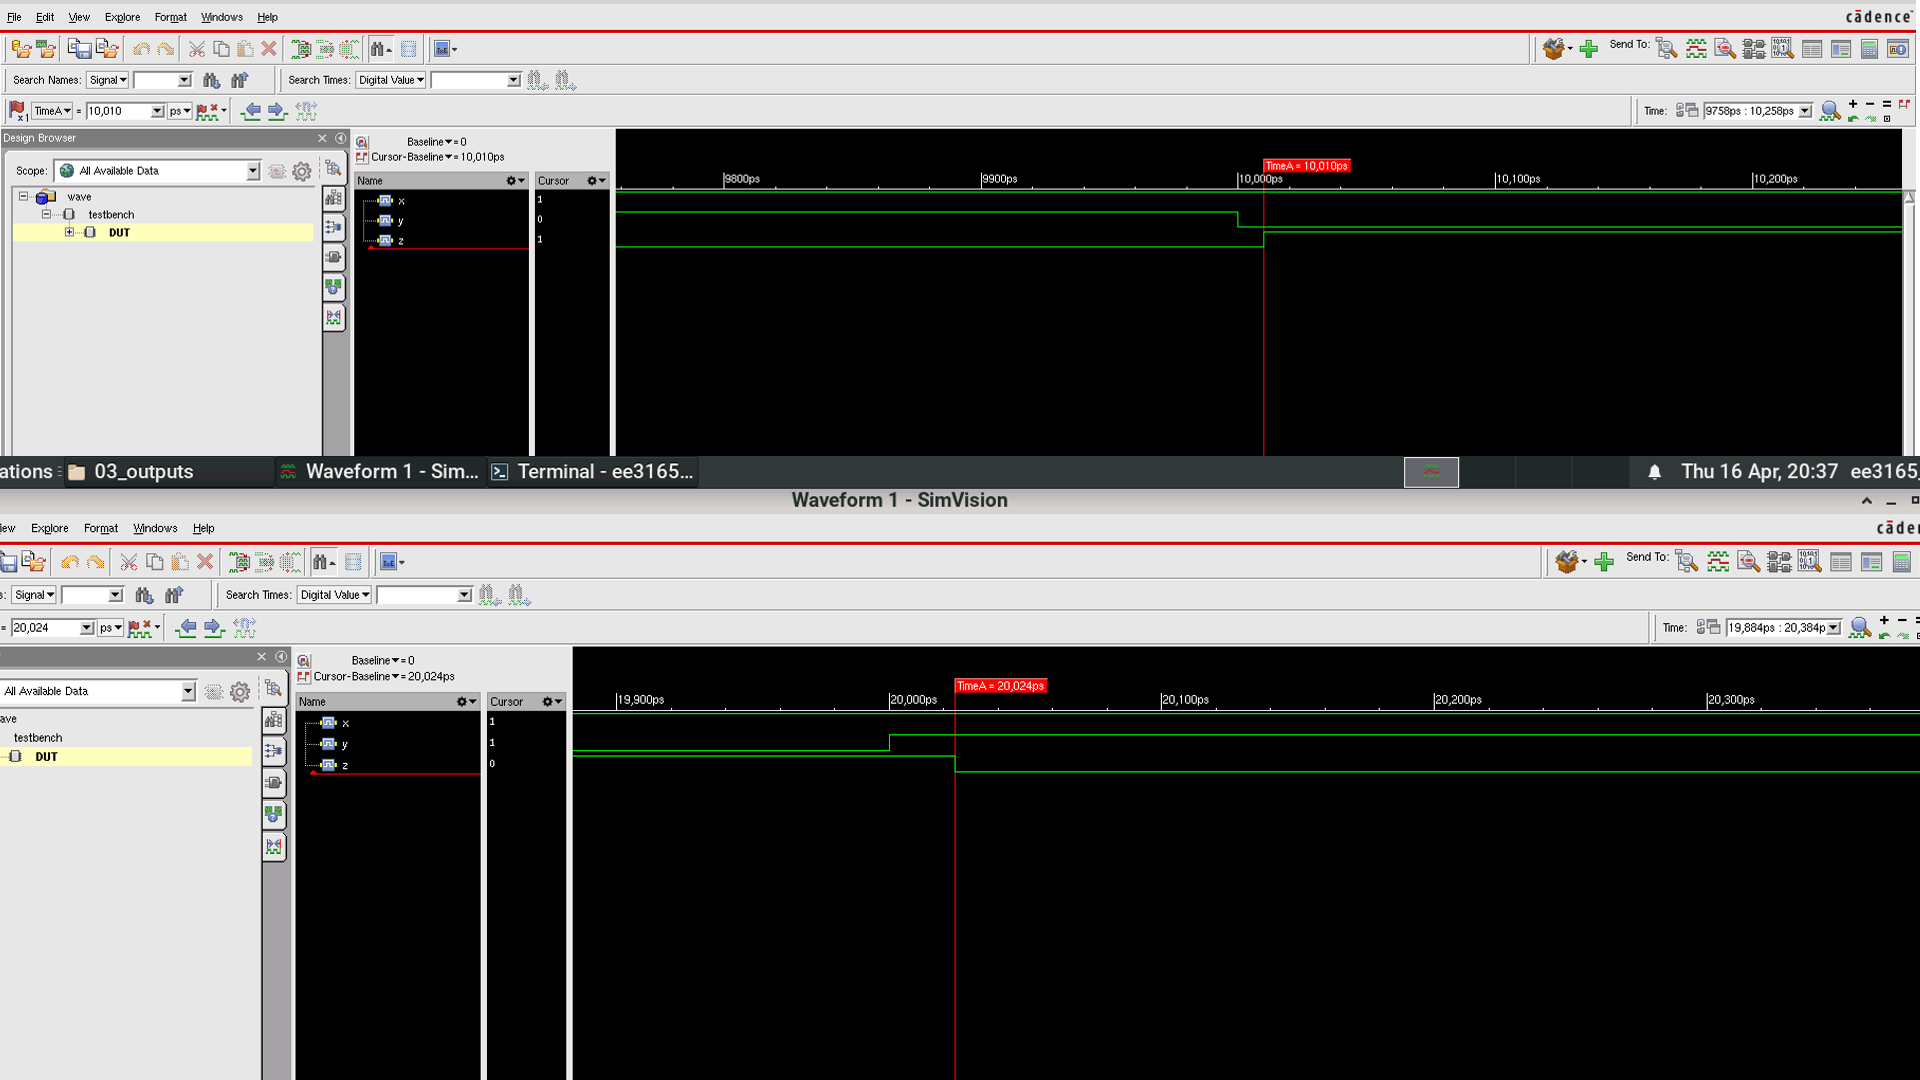
\includegraphics[width=\textwidth]{figures/exp1_nand2_lvt_slow_1v0.png}
        \caption{Corner LVT Slow (slow\_vdd1v0)}
        \label{fig:nand2_lvt_slow_1v0}
    \end{subfigure}
    \caption{Waveform đo độ trễ cổng NAND2 sử dụng thư viện LVT tại 1.0V.}
    \label{fig:nand2_lvt_comparison_1v0}
\end{figure}

\textbf{Nhận xét đặc tính LVT tại 1.0V:}
\begin{itemize}
    \item \textbf{Bù đắp điểm nghẽn vật lý:} Thư viện LVT với điện áp ngưỡng thấp giúp dòng bão hòa vẫn duy trì ở mức cao dù điện áp nguồn chỉ 1.0V. Bằng chứng là độ trễ sườn xuống của chân A tại góc chậm nhất đã giảm mạnh từ $0.066ns$ (của HVT) xuống chỉ còn $0.024ns$, tăng tốc độ chuyển mạch lên gần ba lần.
    \item \textbf{Đánh đổi về rò rỉ điện năng:} Để có được tốc độ này, dòng rò dưới ngưỡng luôn thường trực khiến tổng công suất tiêu thụ của góc chậm nhất là $7.73 \times 10^{-9}W$, nhỉnh hơn một chút so với HVT.
\end{itemize}

\textbf{Khảo sát đặc tính LVT tại điều kiện 1.2V (Điện áp danh định):}

Để xác định hiệu năng cực hạn của cổng NAND2, nhóm thực hiện mô phỏng tại mức điện áp 1.2V với thư viện LVT.

\begin{figure}[H]
    \centering
    \begin{subfigure}[b]{0.48\textwidth}
        \centering
        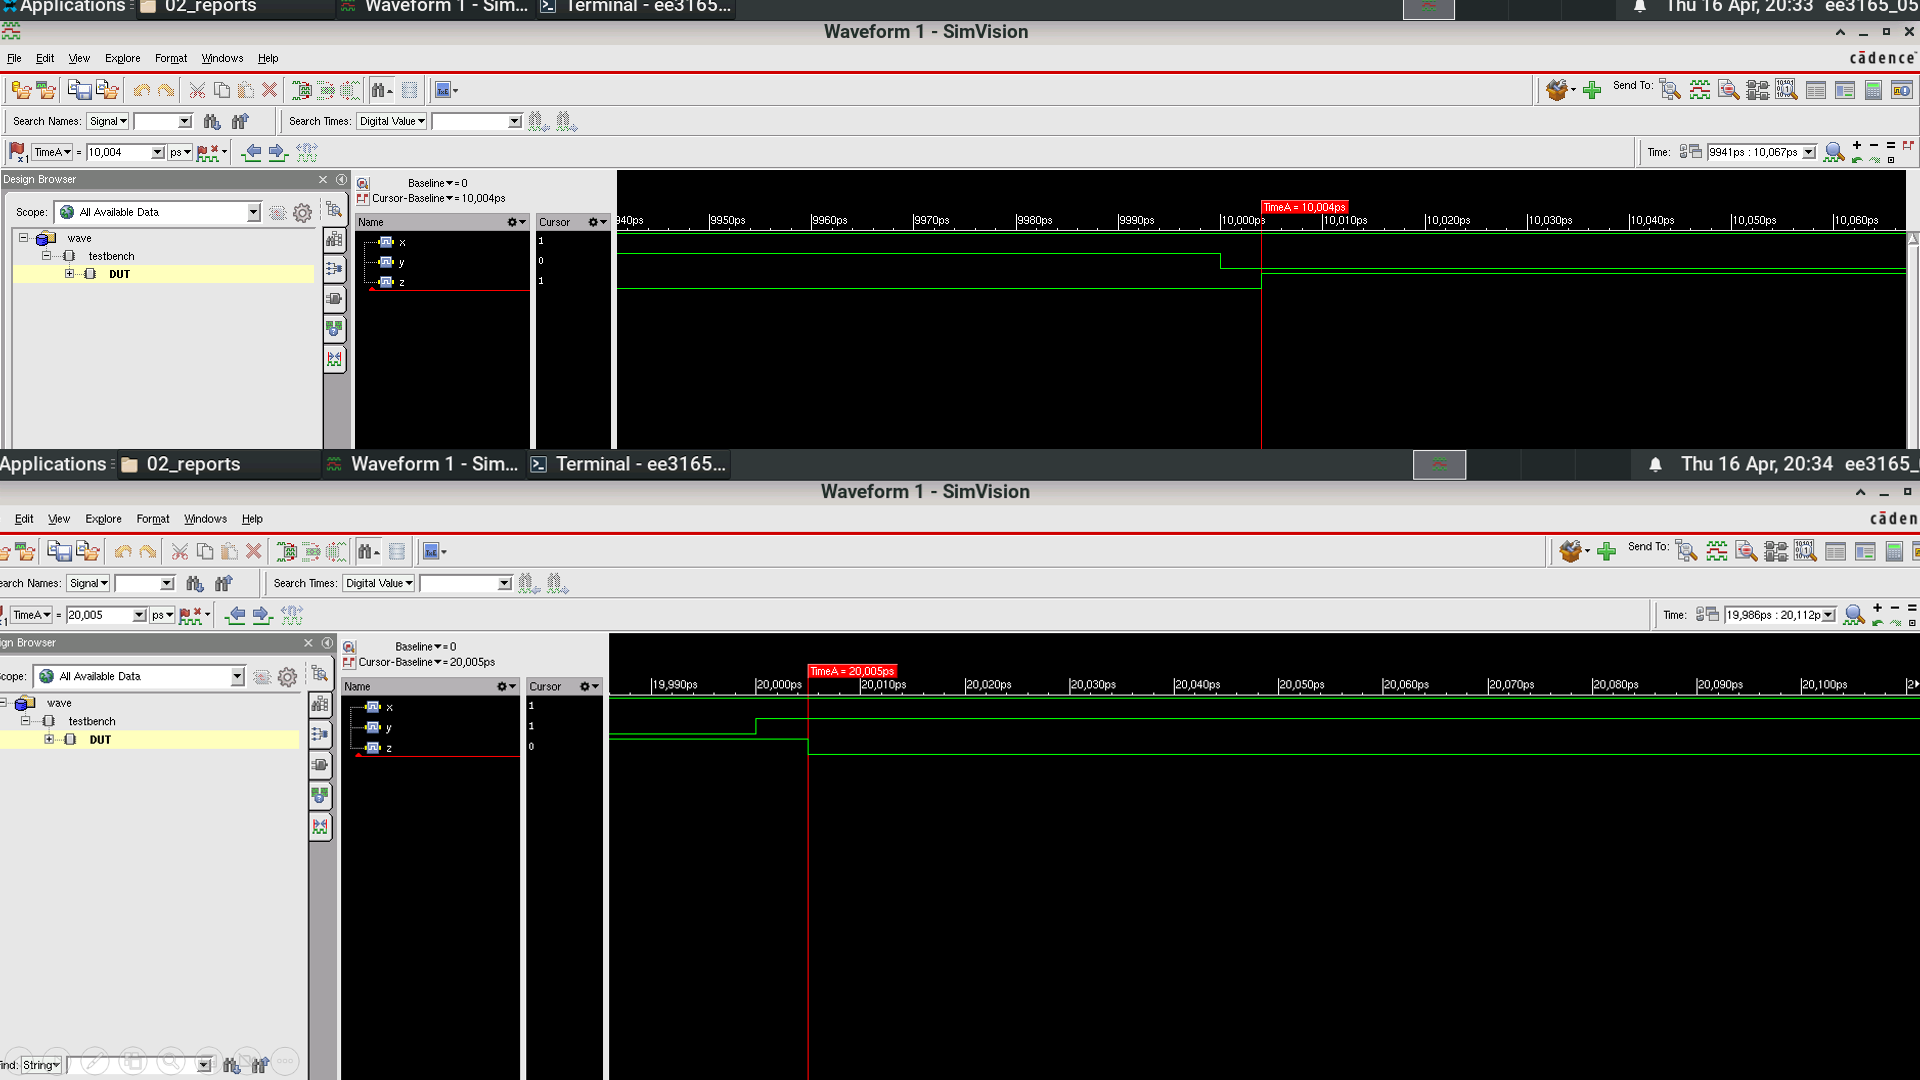
\includegraphics[width=\textwidth]{figures/exp1_nand2_lvt_fast_1v2.png}
        \caption{Corner LVT Fast (fast\_vdd1v2)}
        \label{fig:nand2_lvt_fast_1v2}
    \end{subfigure}
    \hfill
    \begin{subfigure}[b]{0.48\textwidth}
        \centering
        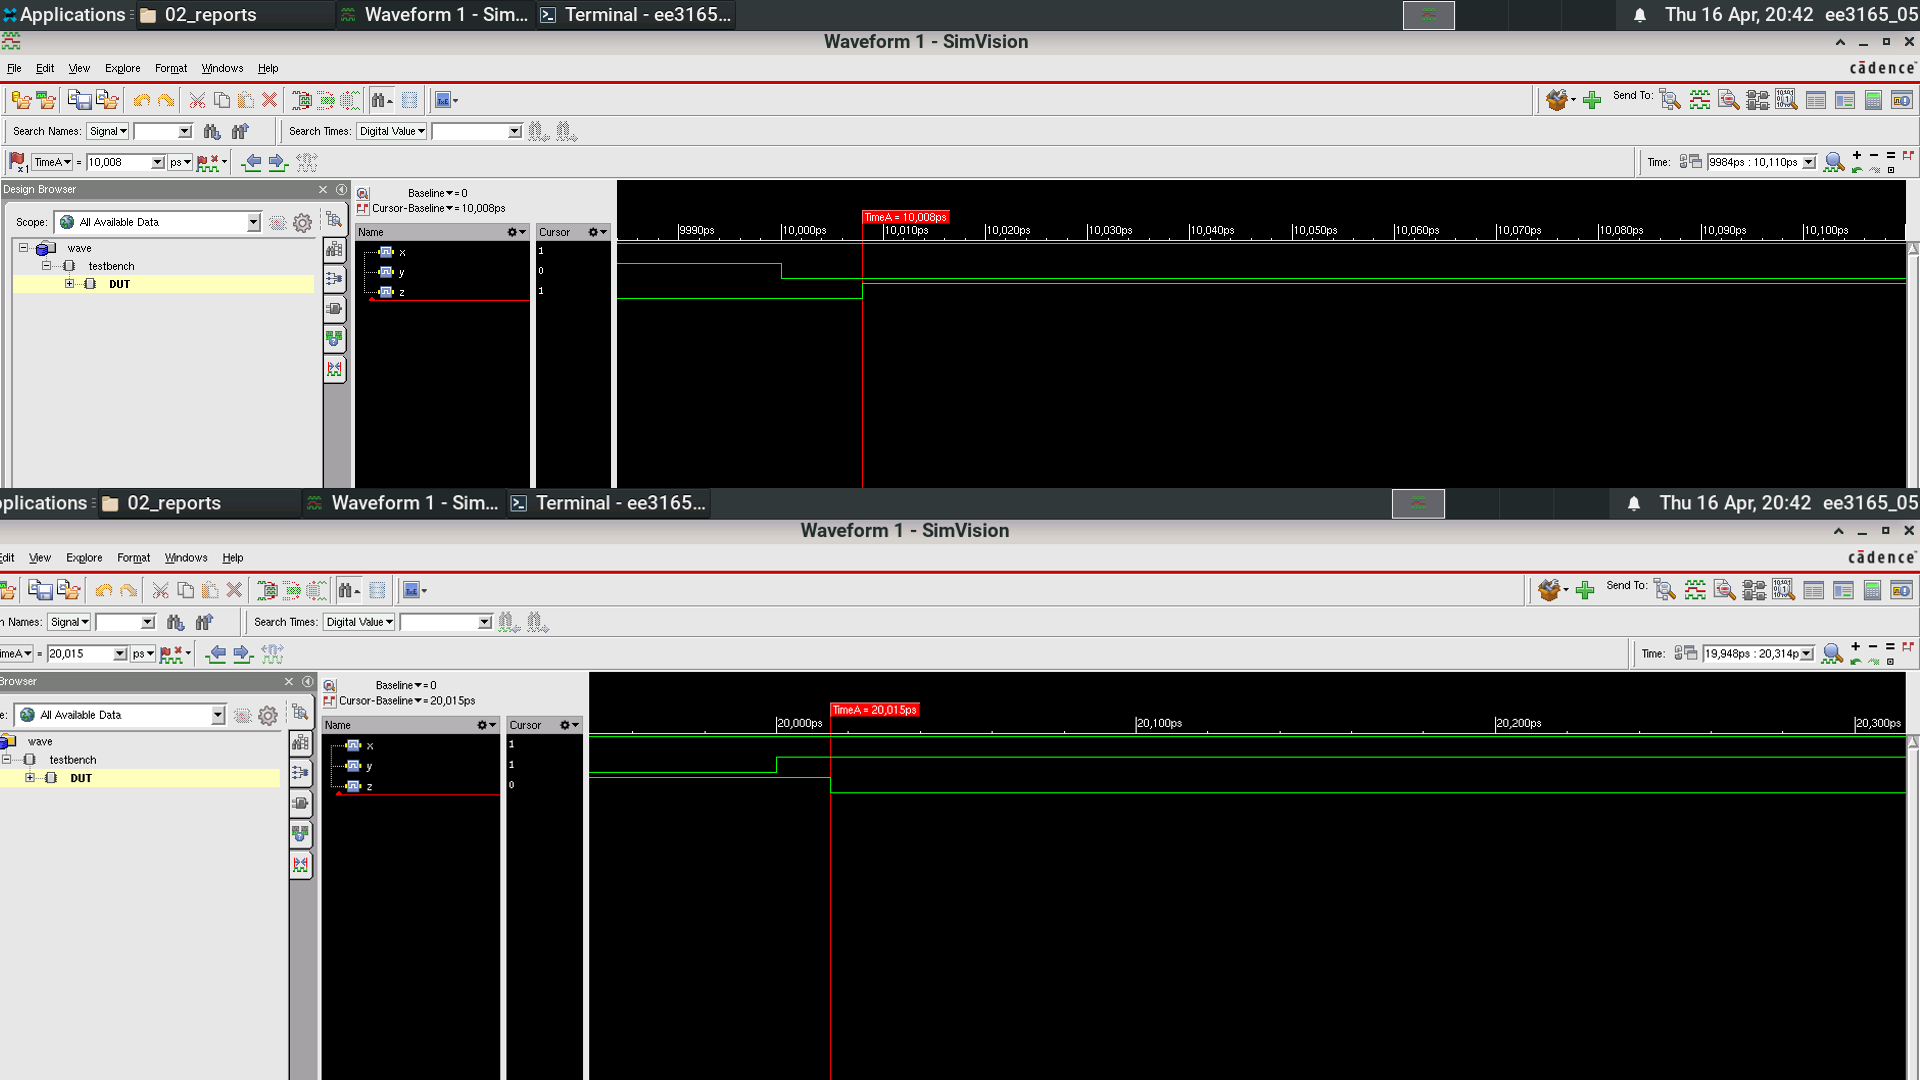
\includegraphics[width=\textwidth]{figures/exp1_nand2_lvt_slow_1v2.png}
        \caption{Corner LVT Slow (slow\_vdd1v2)}
        \label{fig:nand2_lvt_slow_1v2}
    \end{subfigure}
    \caption{Waveform đo độ trễ cổng NAND2 sử dụng thư viện LVT tại 1.2V.}
    \label{fig:nand2_lvt_comparison_1v2}
\end{figure}

\textbf{Nhận xét đặc tính LVT tại 1.2V:}
\begin{itemize}
    \item \textbf{Hiệu năng tối đa:} Tại góc vận hành nhanh nhất, cổng NAND2 đạt thời gian đáp ứng lý tưởng. Sườn lên của chân B chỉ mất $0.003ns$, cho thấy khả năng nạp tụ cực kỳ mạnh mẽ của mạng PMOS song song.
    \item \textbf{Giới hạn công suất:} Đây là điều kiện tiêu tốn năng lượng nhất toàn bộ bài đo cổng NAND2, đạt mốc $2.0 \times 10^{-8}W$. Do đó, bộ tổng hợp mạch chỉ sử dụng cell này khi có yêu cầu khắt khe về thời gian thiết lập.
\end{itemize}

\paragraph{C. Kết luận} 
Phân tích cổng NAND2 tái khẳng định quy luật thiết kế mạch CMOS: diện tích cell là bất biến (luôn cố định ở $1.026 \mu m^2$), trong khi tốc độ và công suất luôn đánh đổi trực tiếp cho nhau. Nhờ kiến trúc PMOS song song, cổng NAND2 có tốc độ sườn lên rất tốt nhưng gặp trở ngại ở sườn xuống do NMOS mắc nối tiếp. Để cân bằng thiết kế, công cụ tự động sẽ ưu tiên sử dụng cổng NAND2 HVT làm nền tảng chính, và chỉ thay thế bằng LVT tại các đường dẫn bị lỗi thời gian.
\newpage
\subsubsection{NOR2}
\begin{lstlisting}[style={prettyverilog}, caption={\texttt{code thiết kế cổng NOR}}]
`timescale 1ns/1ps
module nor(
    input logic A,
    input logic B,
      output logic Y);
    assign Y = ~(A | B);
endmodule
\end{lstlisting}
\begin{lstlisting}[style={prettyverilog}, caption={\texttt{code testbench cổng NOR}}]
`timescale 1ns/1ps
module tb_nor;
    logic A, B;
    logic Y;
    nor(.A(A), .B(B), .Y(Y));
    initial begin
        $dumpfile("nor_wave.vcd");
        $dumpvars(0, tb_nor);
        A = 0; B = 1; #10;
        A = 0; B = 0; #10;
        A = 0; B = 1; #10;
        A = 1; B = 0; #10;
        A = 0; B = 0; #10;
        A = 1; B = 0; #10;
        $finish;
    end
endmodule
\end{lstlisting}

Trước hết, để tổng quan về linh kiện, Hình \ref{fig:exp1_nor2} trình bày ký hiệu logic cơ bản của cổng NOR2. Linh kiện này thực hiện hàm logic đảo của cổng OR, với phương trình đại số Boole $Y = \overline{A + B}$ (ngõ ra chỉ ở mức 1 khi cả hai ngõ vào đồng thời ở mức 0, các trường hợp còn lại ngõ ra đều ở mức 0).

\begin{figure}[H]
    \centering
    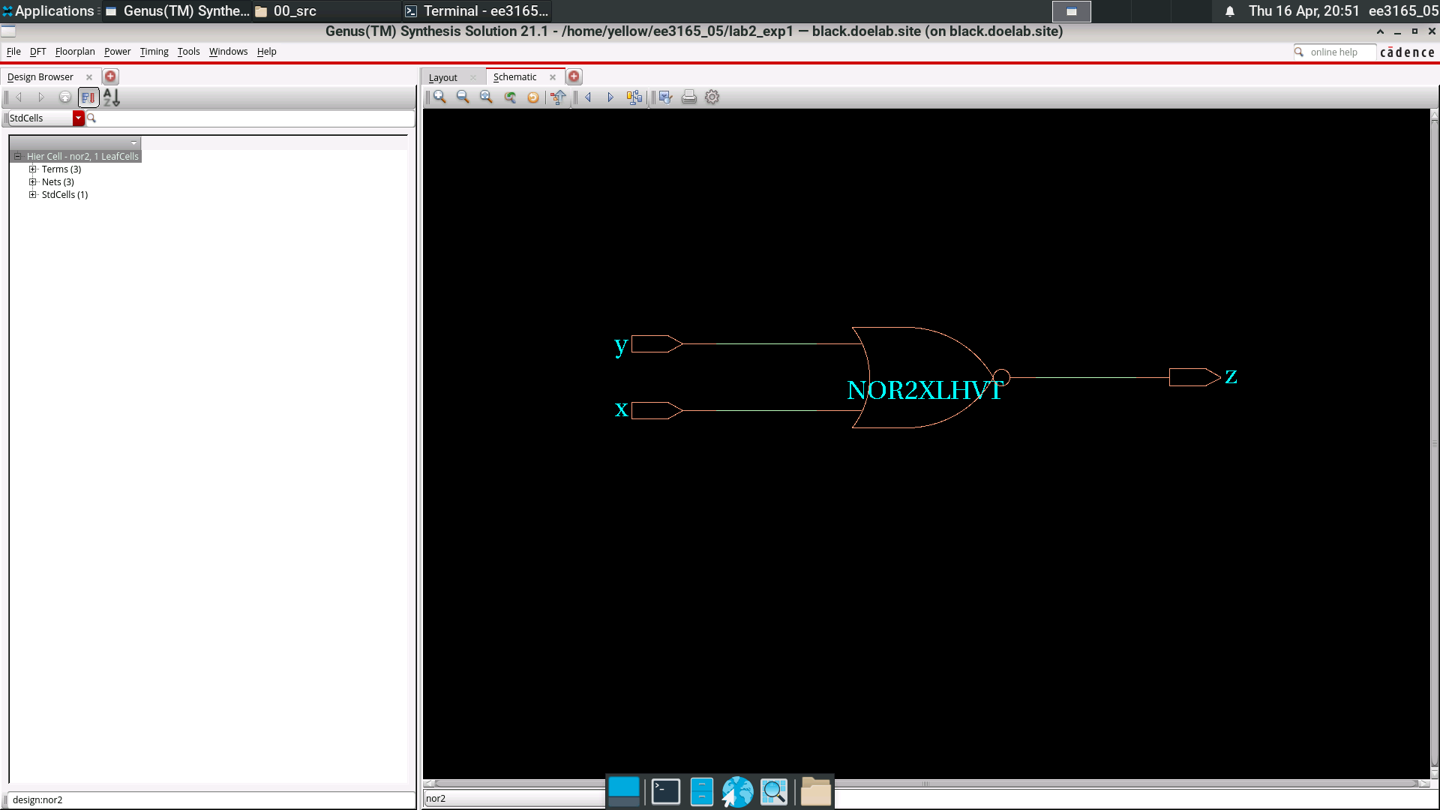
\includegraphics[width=0.6\textwidth]{figures/exp1_nor2.png}
    \caption{Ký hiệu logic và đặc tính cơ bản của cổng NOR2.}
    \label{fig:exp1_nor2}
\end{figure}

Sau khi viết mã RTL, thiết kế được đưa vào công cụ Genus để thực hiện quá trình tổng hợp. Hình \ref{fig:exp1_nor2_mapped} minh họa sơ đồ mức cổng của cổng NOR2 sau khi được ánh xạ vào thư viện công nghệ 45nm.

\begin{figure}[H]
    \centering
    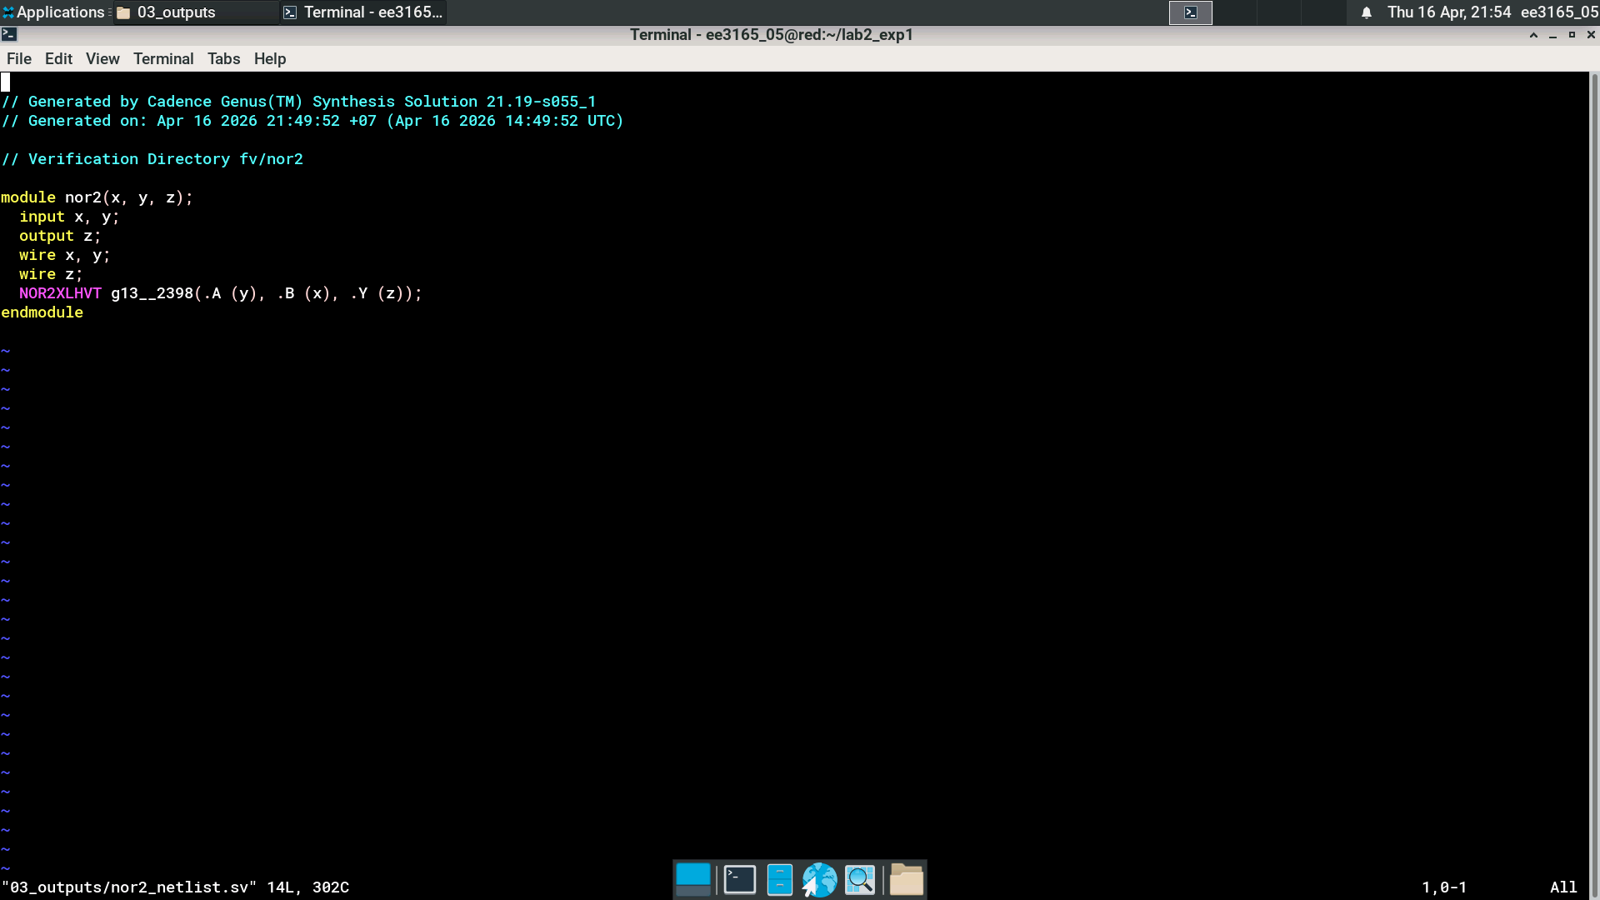
\includegraphics[width=0.7\textwidth]{figures/exp1_nor2_mapped.png}
    \caption{Sơ đồ mức cổng của thiết kế NOR2 trên giao diện Genus.}
    \label{fig:exp1_nor2_mapped}
\end{figure}

Nhóm tiếp tục thực hiện khảo sát đặc tính của cổng NOR2 trên cả hai loại thư viện: High Threshold Voltage (HVT) và Low Threshold Voltage (LVT).

\paragraph{A. Thư viện High Threshold Voltage (HVT)}
Đặc tính của các cell HVT là dòng rò thấp nhưng độ trễ lớn hơn. Kết quả mô phỏng 8 góc quy trình được tổng hợp trong bảng dưới đây:

\begin{table}[H]
\centering
\renewcommand{\arraystretch}{1.3}
\resizebox{\textwidth}{!}{
\begin{tabular}{|l|c|c|c|c|c|c|}
\hline
 
\multirow{2}{*}{\textbf{Library Name}} 
& \multirow{2}{*}{\textbf{Total Area}} 
& \multirow{2}{*}{\textbf{Total Power}} 
 
& \multicolumn{2}{c|}{\textbf{Delay Parameter A$\rightarrow$Y}}
& \multicolumn{2}{c|}{\textbf{Delay Parameter B$\rightarrow$Y}} \\
 
\cline{4-7}
 
& & 
& \textbf{Rising Delay (ns)} 
& \textbf{Falling Delay (ns)}
& \textbf{Rising Delay (ns)} 
& \textbf{Falling Delay (ns)} \\
 
\hline
 
% ----------- KHỐI HVT ----------------
 
fast\_vdd1v0\_basicCells\_hvt 
& 1.026 & 1.07544e-08 
& 0.011 & 0.007
& 0.008 & 0.005 \\ \hline
 
fast\_vdd1v2\_basicCells\_hvt 
& 1.026 & 1.56633e-08 
& 0.009 & 0.006
& 0.006 & 0.004 \\ \hline
 
slow\_vdd1v0\_basicCells\_hvt 
& 1.026 & 7.30888e-09 
& 0.036 & 0.030
& 0.025 & 0.020 \\ \hline
 
slow\_vdd1v2\_basicCells\_hvt 
& 1.026 & 1.06519e-08 
& 0.019 & 0.016
& 0.013 & 0.010 \\ \hline

\end{tabular}
}

\caption{Tổng hợp thông số Diện tích, Công suất và Độ trễ của cổng NOR2 (HVT).}
\label{tab:exp1_nor2_hvt_params}

\end{table}

Dưới đây là sự so sánh dạng sóng mô phỏng của cổng NOR2 tại hai góc cực đoan ở cùng mức điện áp 1.0V. Các hình ảnh dạng sóng trong phần này được trích xuất đại diện cho đường dẫn tín hiệu từ ngõ vào A đến ngõ ra Y.

\begin{figure}[H]
    \centering
    \begin{subfigure}[b]{0.48\textwidth}
        \centering
        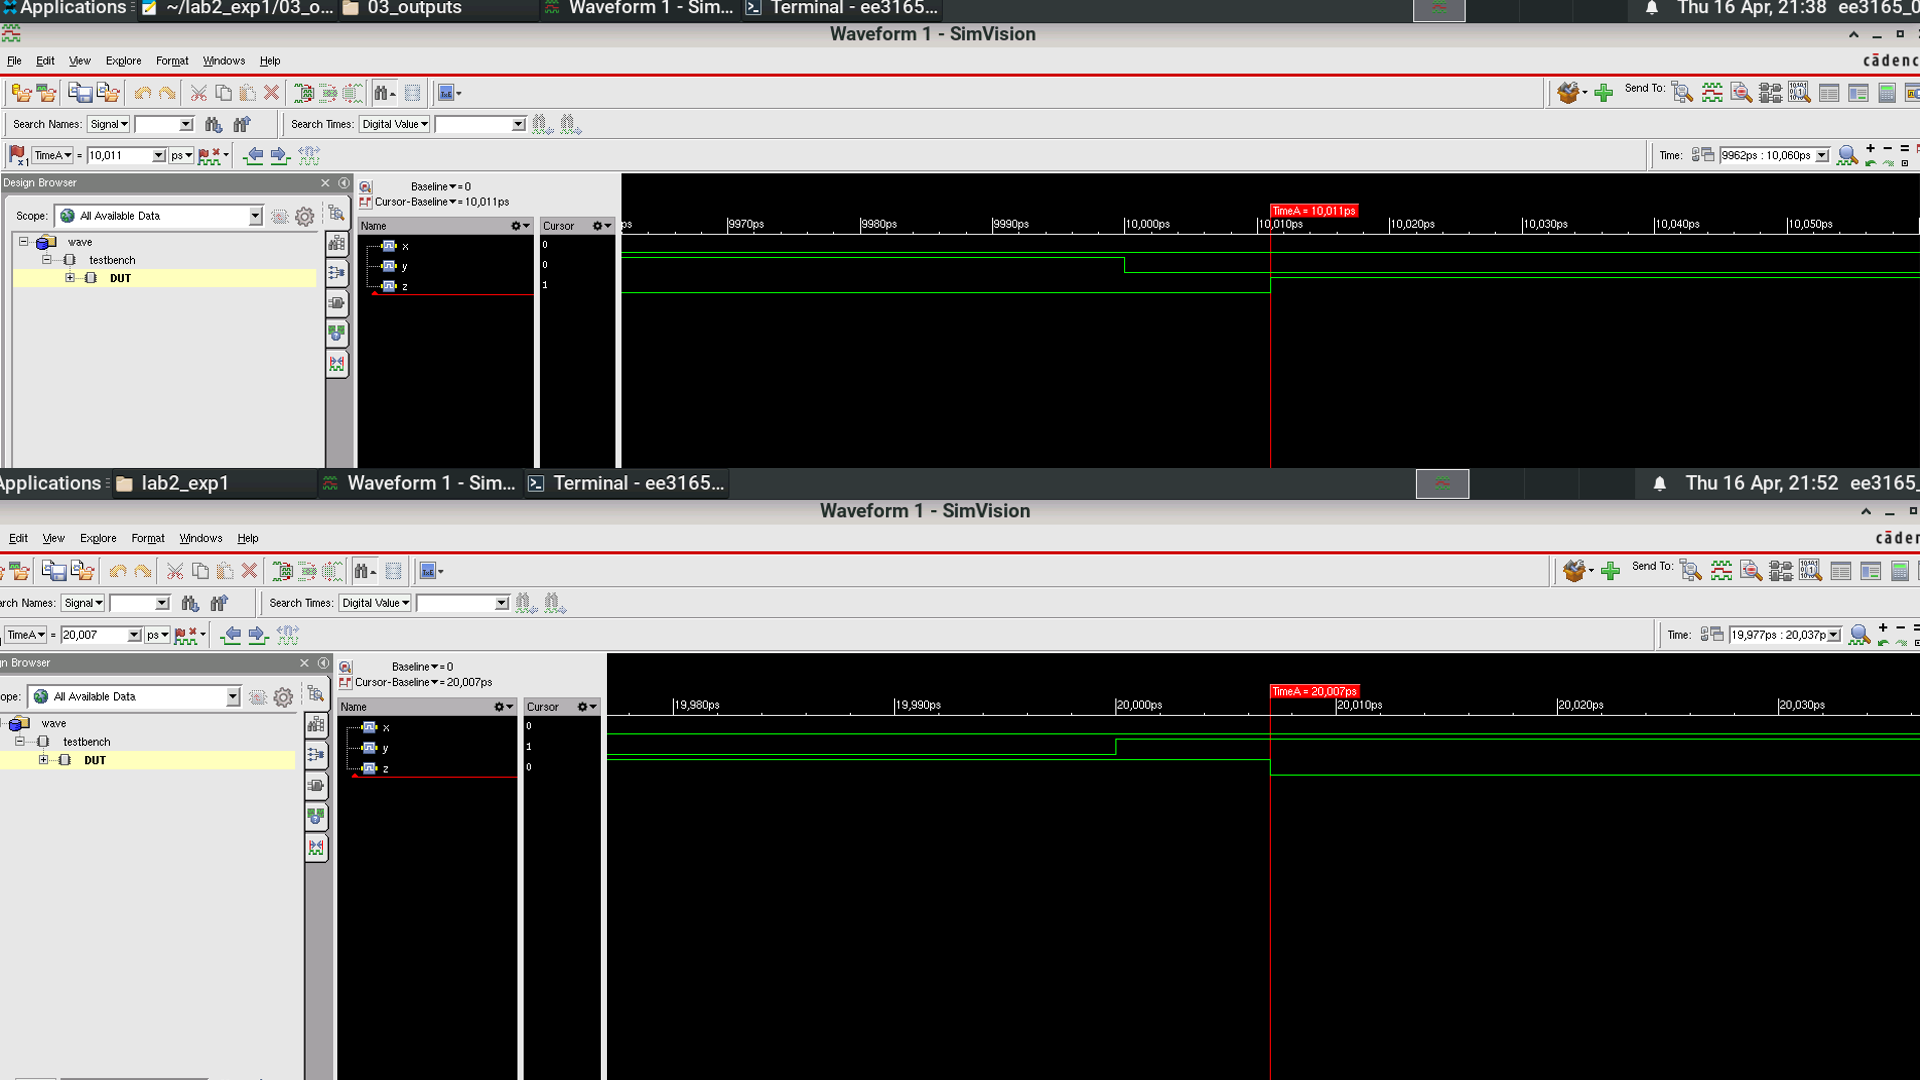
\includegraphics[width=\textwidth]{figures/exp1_nor2_hvt_fast_1v0.png}
        \caption{Góc HVT Fast (fast\_vdd1v0)}
    \end{subfigure}
    \hfill
    \begin{subfigure}[b]{0.48\textwidth}
        \centering
        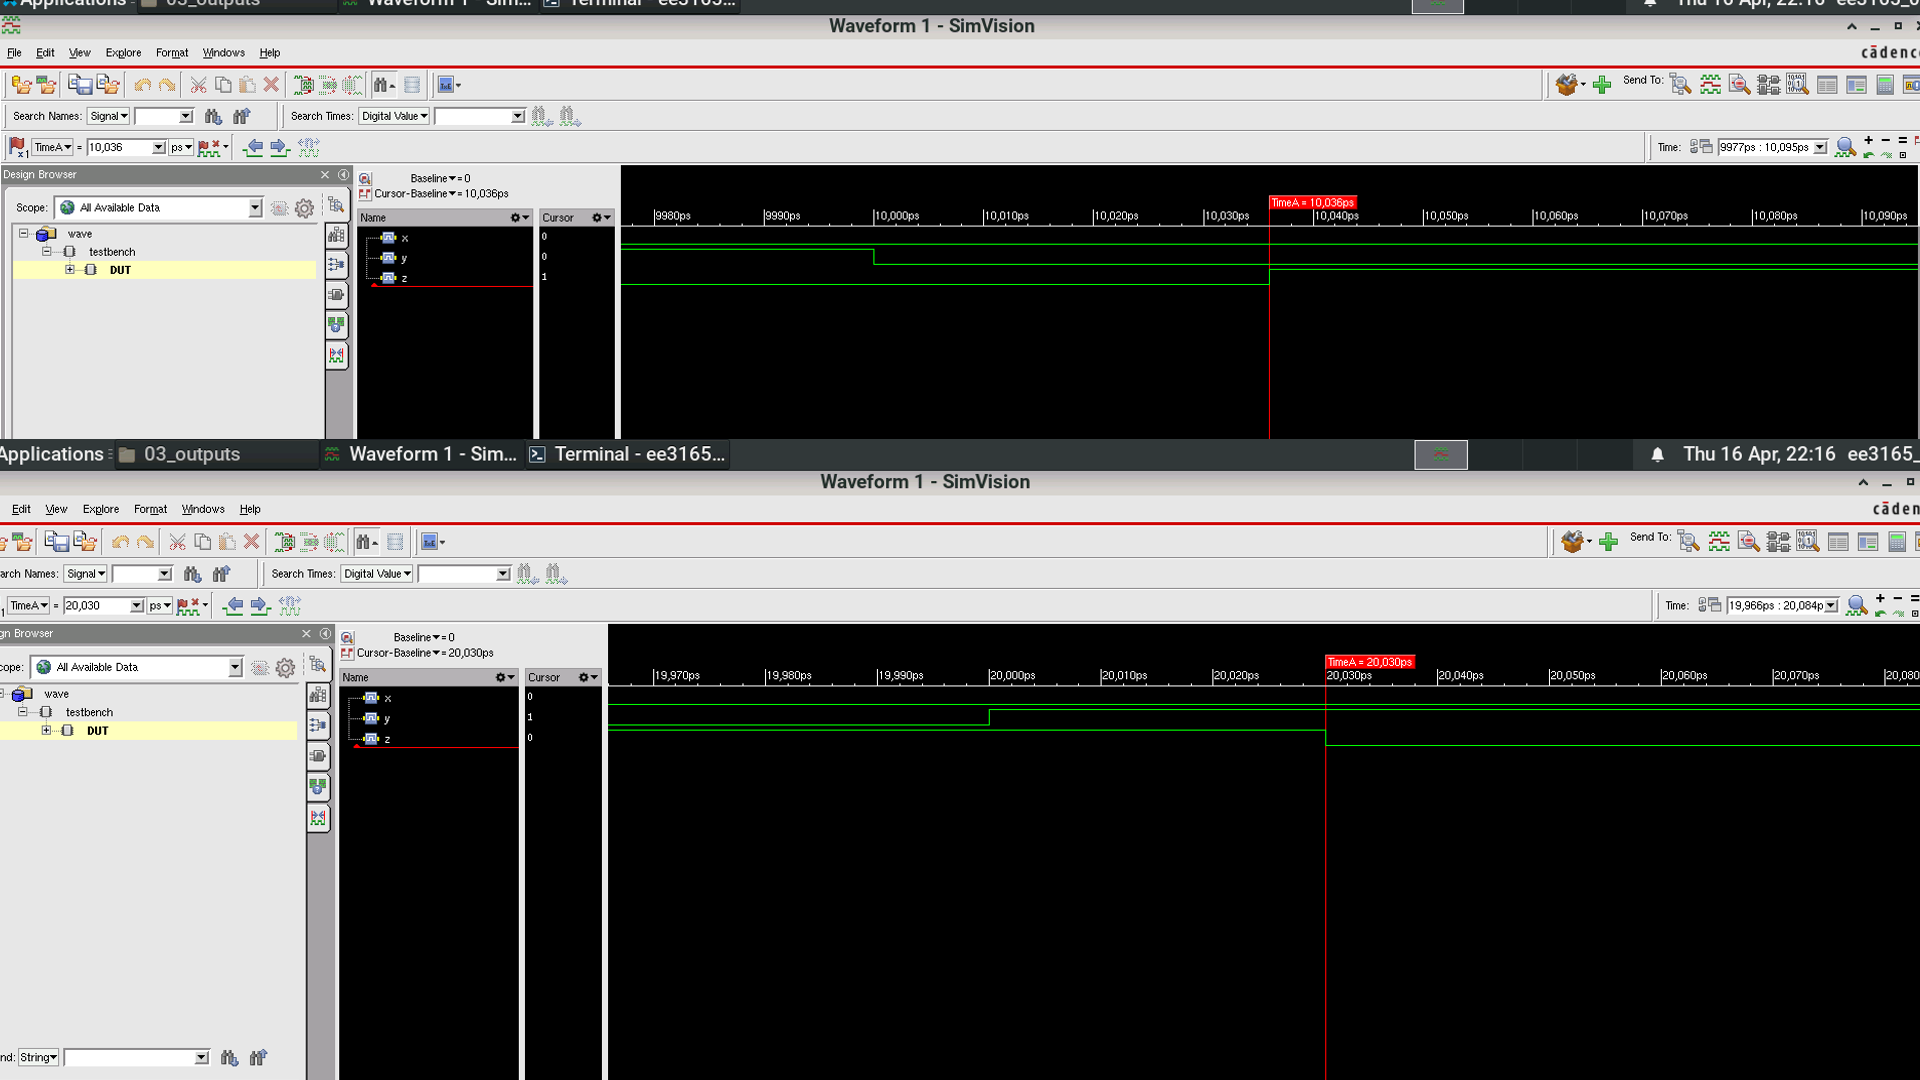
\includegraphics[width=\textwidth]{figures/exp1_nor2_hvt_slow_1v0.png}
        \caption{Góc HVT Slow (slow\_vdd1v0)}
    \end{subfigure}
    \caption{So sánh dạng sóng đo độ trễ cổng NOR2 ở HVT (VDD = 1.0V). Hình ảnh đại diện cho đường dẫn A$\rightarrow$Y.}
    \label{fig:nor2_hvt_comparison_1v0}
\end{figure}

\textbf{Nhận xét (HVT - 1.0V):} Dựa trên số liệu đo đạc tại mức điện áp 1.0V, ta có thể đánh giá chi tiết bản chất vật lý của cổng NOR2:
\begin{itemize}
    \item \textbf{Điểm nghẽn ở mạng kéo lên:} Kiến trúc bên trong của cổng NOR2 bao gồm hai transistor PMOS mắc nối tiếp ở phần mạng kéo lên để nạp điện cho ngõ ra. Do đặc tính vật lý của vật liệu bán dẫn, hạt tải điện trong PMOS (các lỗ trống) có độ linh động kém hơn rất nhiều so với hạt tải điện trong NMOS. Việc mắc nối tiếp hai PMOS làm tăng gấp đôi điện trở tương đương, khiến quá trình nạp tụ diễn ra rất chậm chạp. Bảng số liệu phản ánh rõ điều này: độ trễ sườn lên luôn lớn hơn sườn xuống. Tại góc chậm nhất, độ trễ sườn lên của chân A lên tới $0.036ns$, trong khi sườn xuống chỉ mất $0.030ns$.
    \item \textbf{Độ trễ bất đối xứng giữa các ngõ vào:} Quan sát bảng số liệu, tín hiệu đi từ chân A đến Y ($0.036ns$) mất nhiều thời gian hơn từ chân B đến Y ($0.025ns$). Hiện tượng này xảy ra do sự sắp xếp vật lý của các transistor trên mạch silic. Transistor kết nối với ngõ vào A thường nằm xa nút ngõ ra hơn, tạo ra điện dung và điện trở ký sinh lớn hơn trên đường dẫn tín hiệu.
    \item \textbf{Tối ưu hóa năng lượng tĩnh:} Mặc dù tốc độ bị hạn chế, góc chậm nhất ở 1.0V mang lại hiệu quả tiết kiệm điện cực kỳ tốt. Mức tiêu thụ công suất tĩnh và động tổng hợp chỉ đạt $7.30 \times 10^{-9}W$, biến cấu hình này thành lựa chọn phù hợp cho các khối không yêu cầu khắt khe về thời gian.
\end{itemize}

\vspace{1cm}

Dưới đây là kết quả mô phỏng tại điện áp danh định 1.2V cho thư viện HVT.

\begin{figure}[H]
    \centering
    \begin{subfigure}[b]{0.48\textwidth}
        \centering
        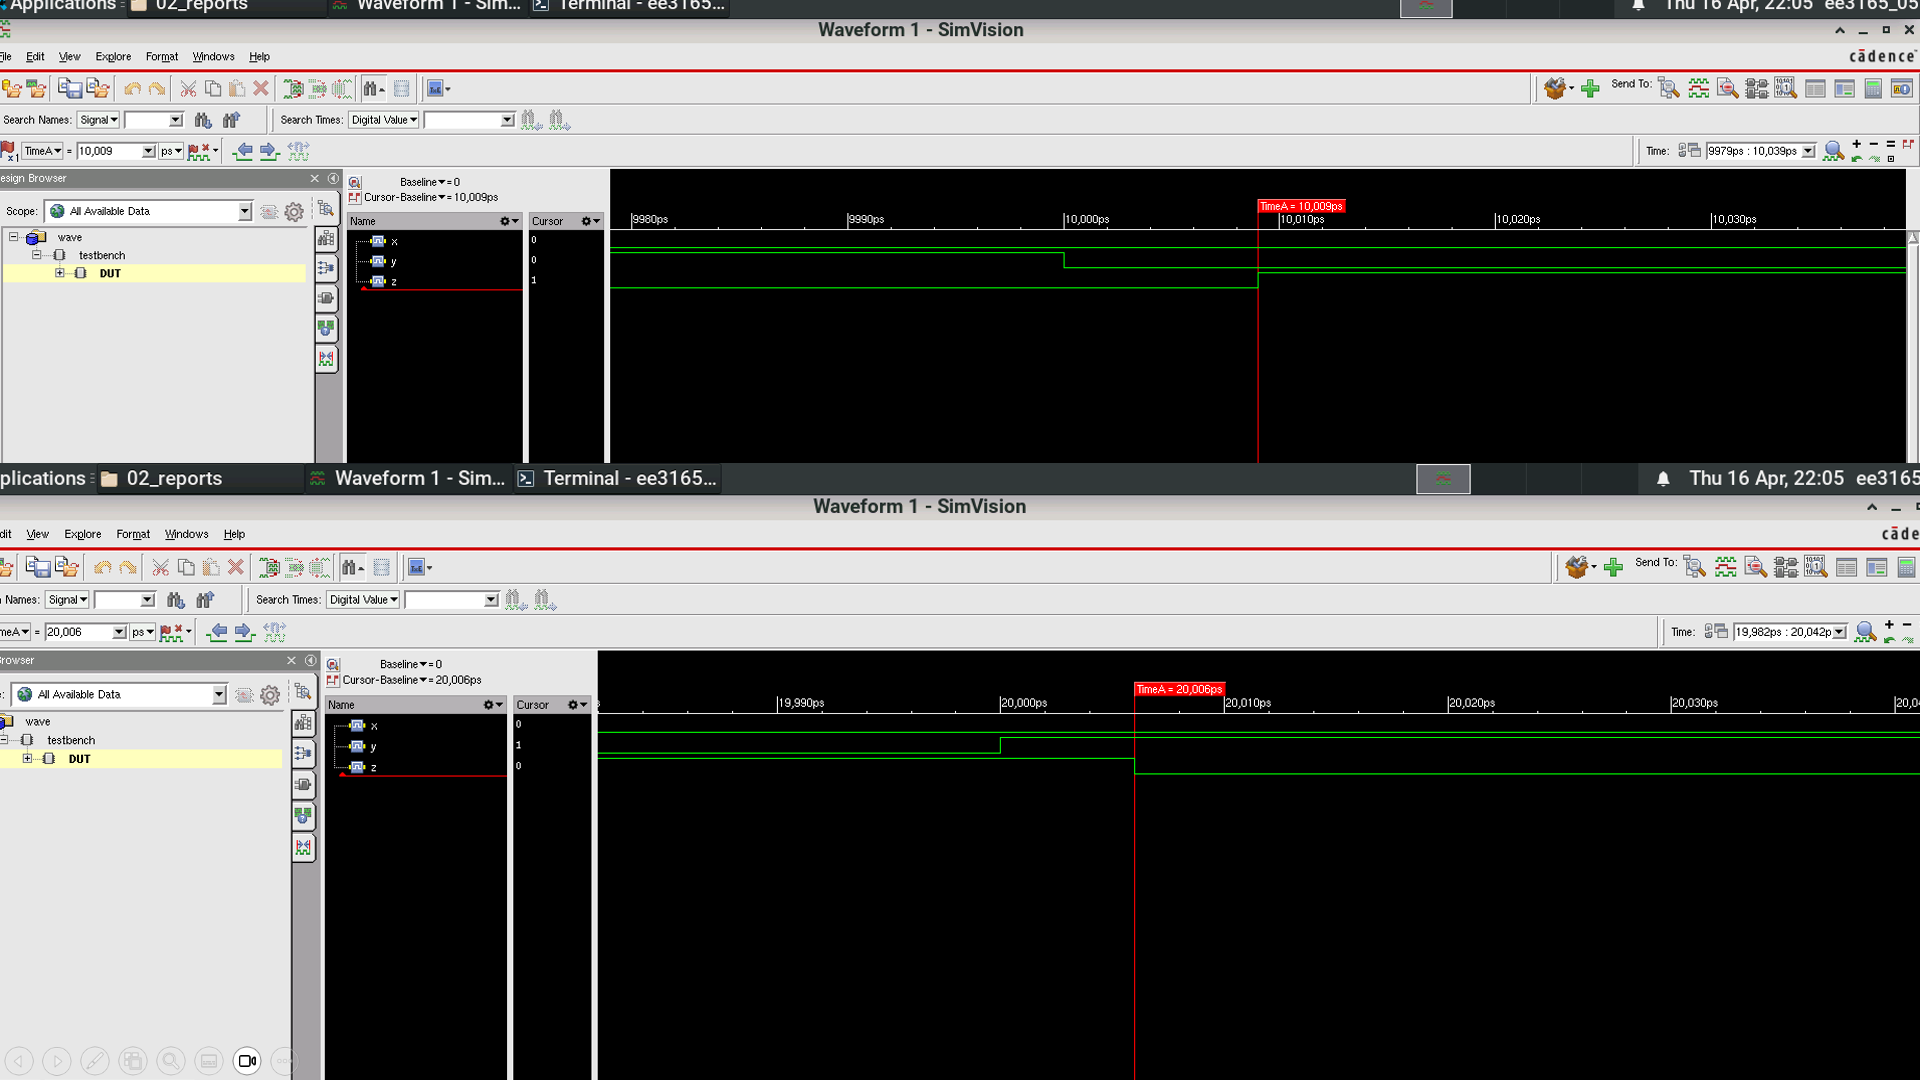
\includegraphics[width=\textwidth]{figures/exp1_nor2_hvt_fast_1v2.png}
        \caption{Góc HVT Fast (fast\_vdd1v2)}
    \end{subfigure}
    \hfill
    \begin{subfigure}[b]{0.48\textwidth}
        \centering
        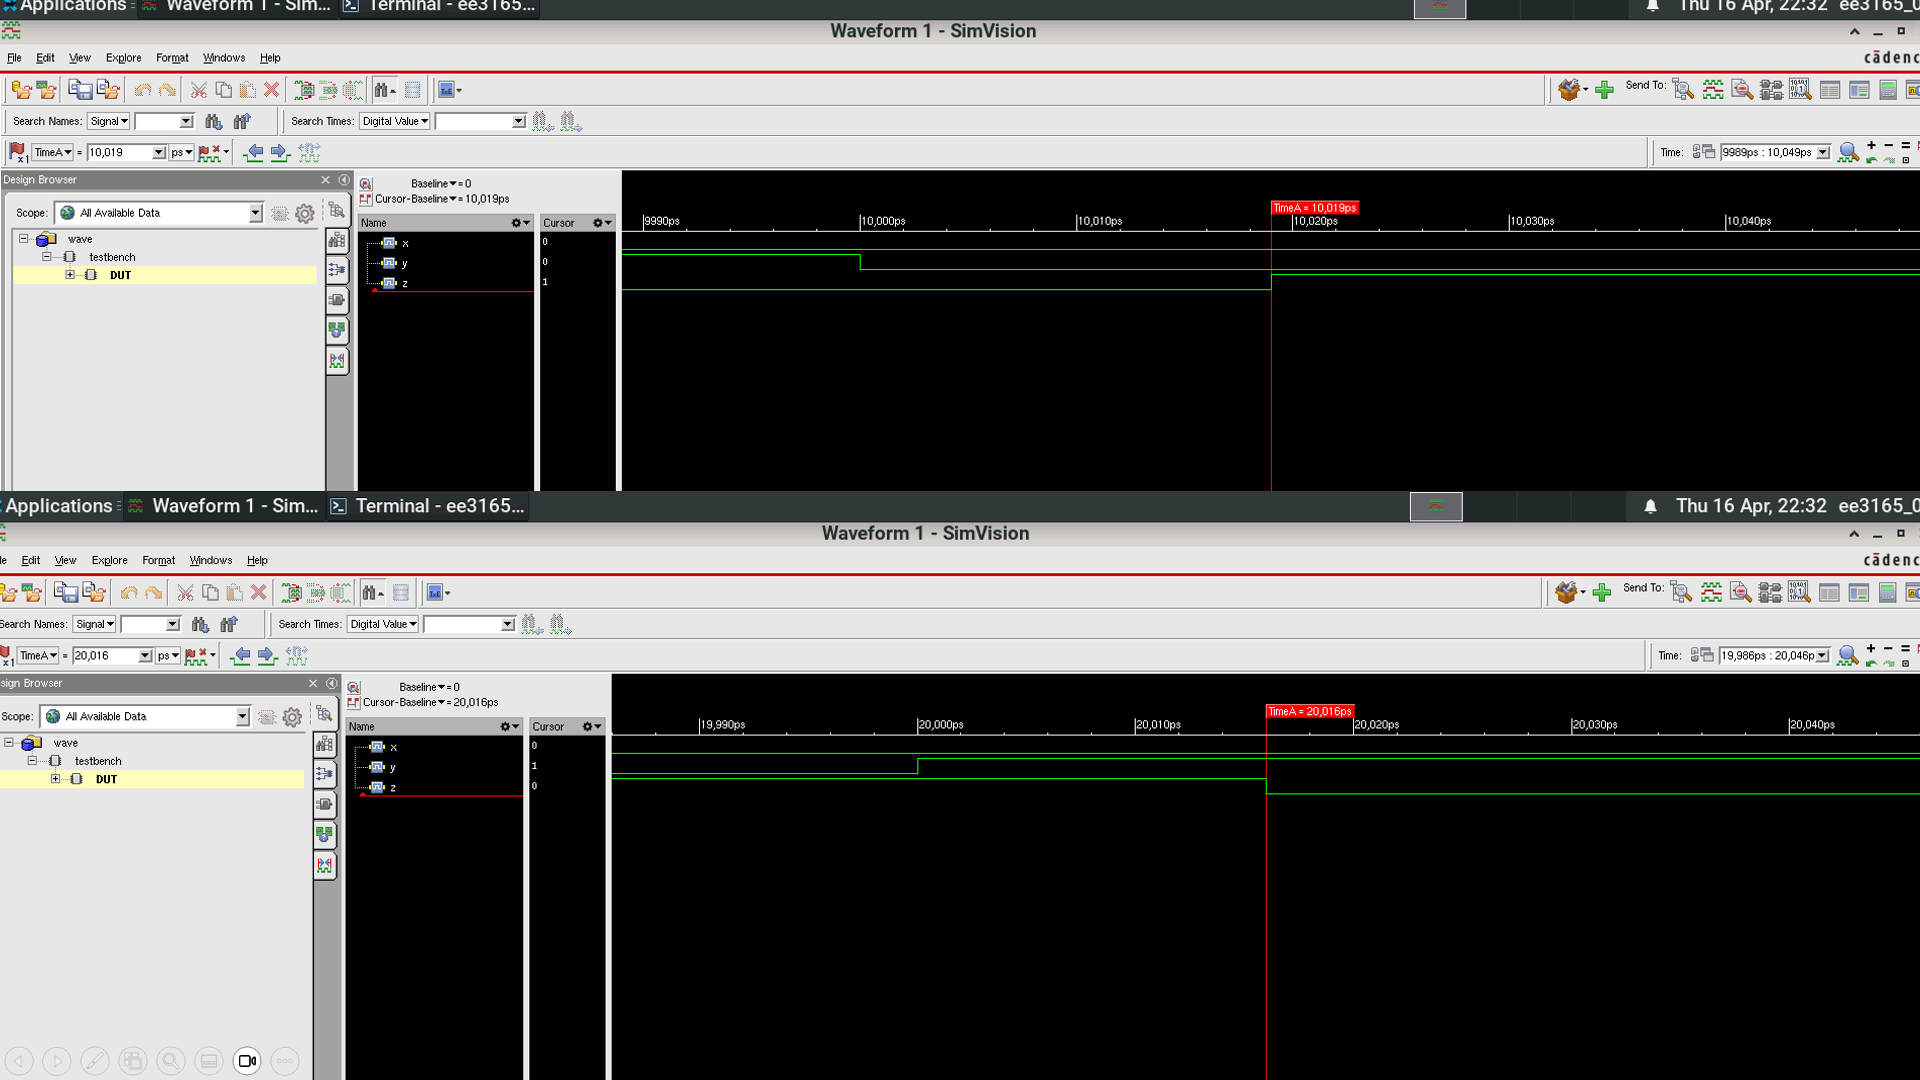
\includegraphics[width=\textwidth]{figures/exp1_nor2_hvt_slow_1v2.png}
        \caption{Góc HVT Slow (slow\_vdd1v2)}
    \end{subfigure}
    \caption{So sánh dạng sóng đo độ trễ cổng NOR2 ở HVT (VDD = 1.2V). Hình ảnh đại diện cho đường dẫn A$\rightarrow$Y.}
    \label{fig:nor2_hvt_comparison_1v2}
\end{figure}

\textbf{Nhận xét (HVT - 1.2V):} Việc cấp đủ mức điện áp 1.2V là giải pháp trực tiếp để cải thiện tốc độ của mạng PMOS mắc nối tiếp:
\begin{itemize}
    \item \textbf{Khắc phục hiện tượng đói dòng:} Sự gia tăng điện áp nguồn giúp gia tăng điện áp quá lái. Dòng điện bão hòa mạnh mẽ hơn giúp thời gian nạp tụ rút ngắn đáng kể. Tại góc nhanh nhất, độ trễ sườn lên của ngõ A giảm chỉ còn $0.009ns$, đáp ứng tốt các yêu cầu về tốc độ xung nhịp.
    \item \textbf{Sự gia tăng công suất động:} Đổi lại sự cải thiện về thời gian, công suất tiêu thụ tại góc nhanh nhất tăng vọt lên mức $1.56 \times 10^{-8}W$. Điều này minh chứng rõ nét cho quy luật công suất động phụ thuộc vào bình phương điện áp nguồn.
\end{itemize}

\paragraph{B. Thư viện Low Threshold Voltage (LVT)}
Các cell LVT cung cấp tốc độ chuyển mạch nhanh hơn nhờ hạ thấp rào cản điện áp ngưỡng, đổi lại công suất tiêu thụ tĩnh do dòng rò sẽ cao hơn.

\begin{table}[H]
\centering
\renewcommand{\arraystretch}{1.3}
\resizebox{\textwidth}{!}{
\begin{tabular}{|l|c|c|c|c|c|c|}
\hline
 
\multirow{2}{*}{\textbf{Library Name}} 
& \multirow{2}{*}{\textbf{Total Area}} 
& \multirow{2}{*}{\textbf{Total Power}} 
 
& \multicolumn{2}{c|}{\textbf{Delay Parameter A$\rightarrow$Y}}
& \multicolumn{2}{c|}{\textbf{Delay Parameter B$\rightarrow$Y}} \\
 
\cline{4-7}
 
& & 
& \textbf{Rising Delay (ns)} 
& \textbf{Falling Delay (ns)}
& \textbf{Rising Delay (ns)} 
& \textbf{Falling Delay (ns)} \\
 
\hline
 
% ----------- KHỐI LVT ----------------
 
fast\_vdd1v0\_basicCells\_lvt 
& 1.026 & 1.44019e-08 
& 0.007 & 0.005
& 0.005 & 0.003 \\ \hline
 
fast\_vdd1v2\_basicCells\_lvt 
& 1.026 & 2.03360e-08 
& 0.006 & 0.004
& 0.004 & 0.003 \\ \hline
 
slow\_vdd1v0\_basicCells\_lvt 
& 1.026 & 7.82275e-09 
& 0.020 & 0.014
& 0.013 & 0.008 \\ \hline
 
slow\_vdd1v2\_basicCells\_lvt 
& 1.026 & 1.13492e-08 
& 0.013 & 0.010
& 0.008 & 0.006 \\ \hline
 
\end{tabular}
}

\caption{Tổng hợp thông số Diện tích, Công suất và Độ trễ của NOR2 (LVT).}
\label{tab:exp1_nor2_lvt_params}

\end{table}

\textbf{Khảo sát đặc tính LVT tại điều kiện 1.0V (Điện áp thấp):}

\begin{figure}[H]
    \centering
    \begin{subfigure}[b]{0.48\textwidth}
        \centering
        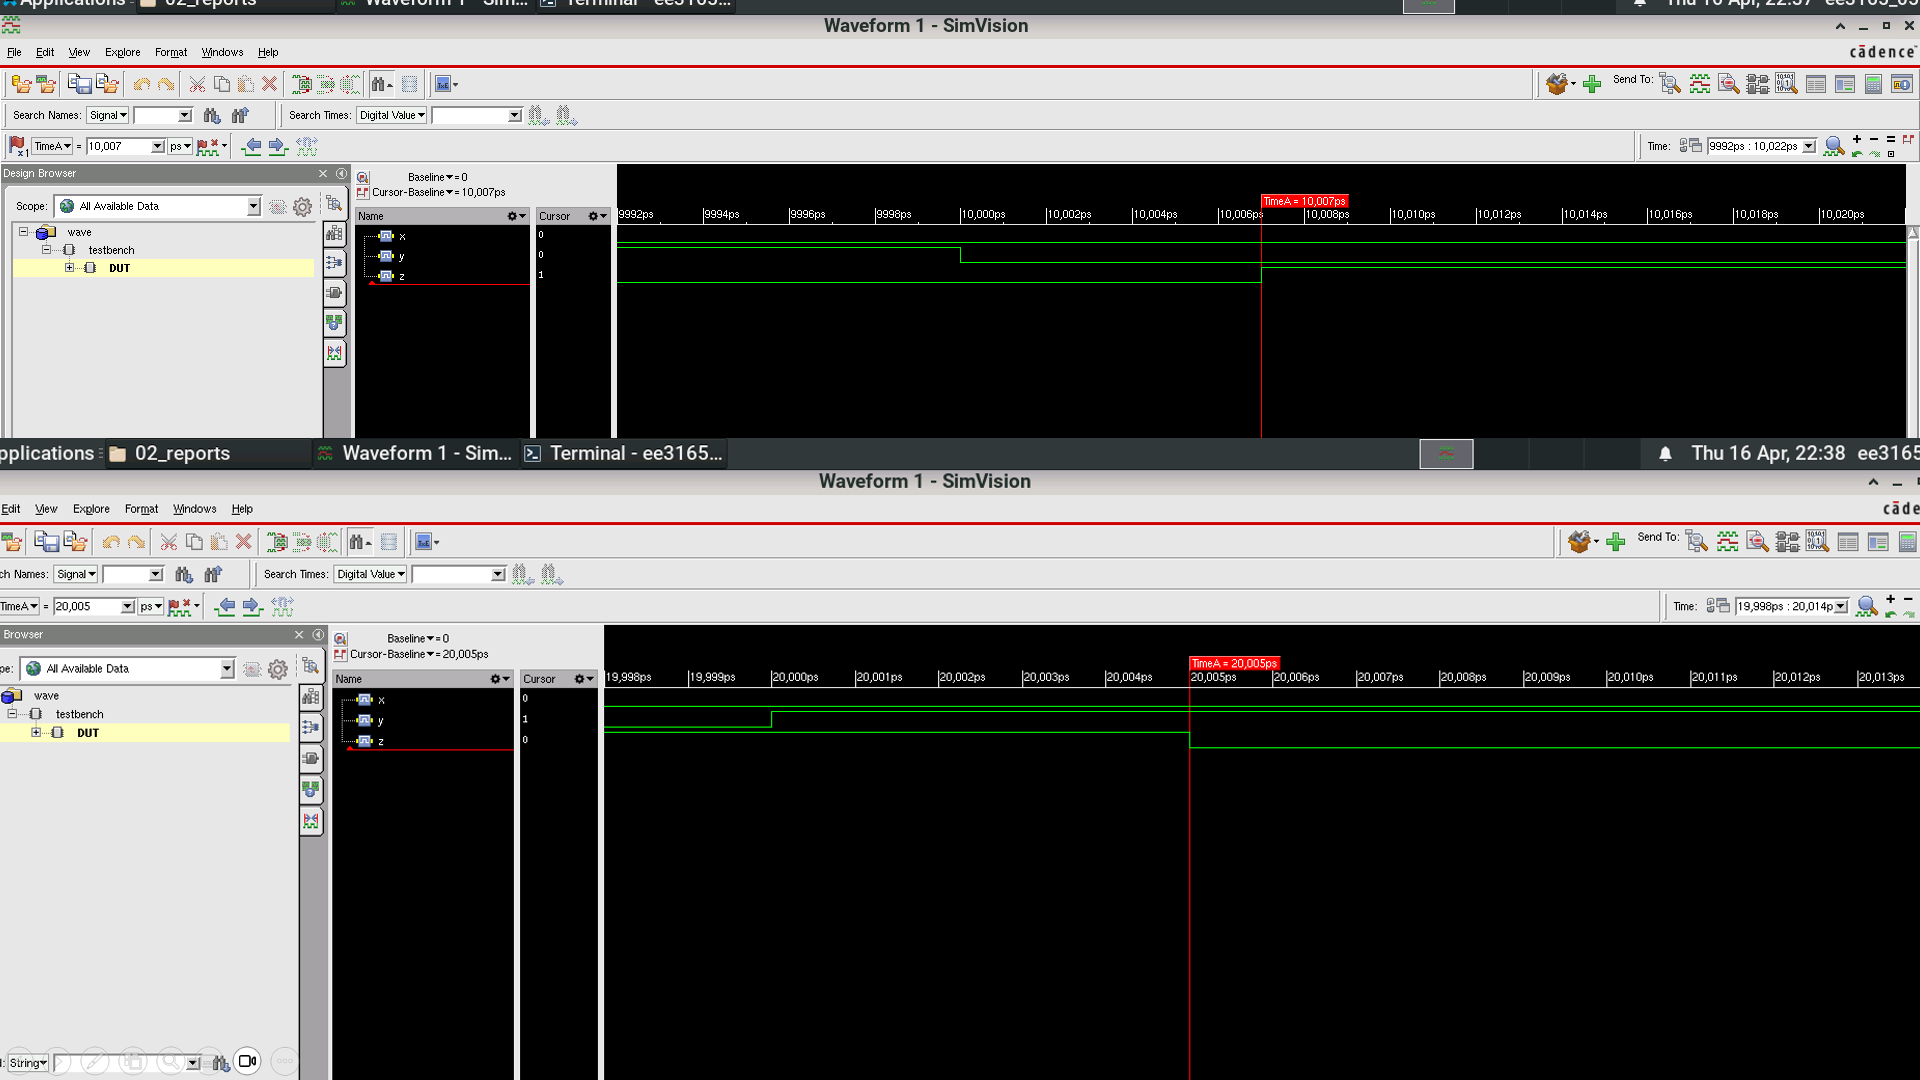
\includegraphics[width=\textwidth]{figures/exp1_nor2_lvt_fast_1v0.png}
        \caption{Góc LVT Fast (fast\_vdd1v0)}
        \label{fig:nor2_lvt_fast_1v0}
    \end{subfigure}
    \hfill
    \begin{subfigure}[b]{0.48\textwidth}
        \centering
        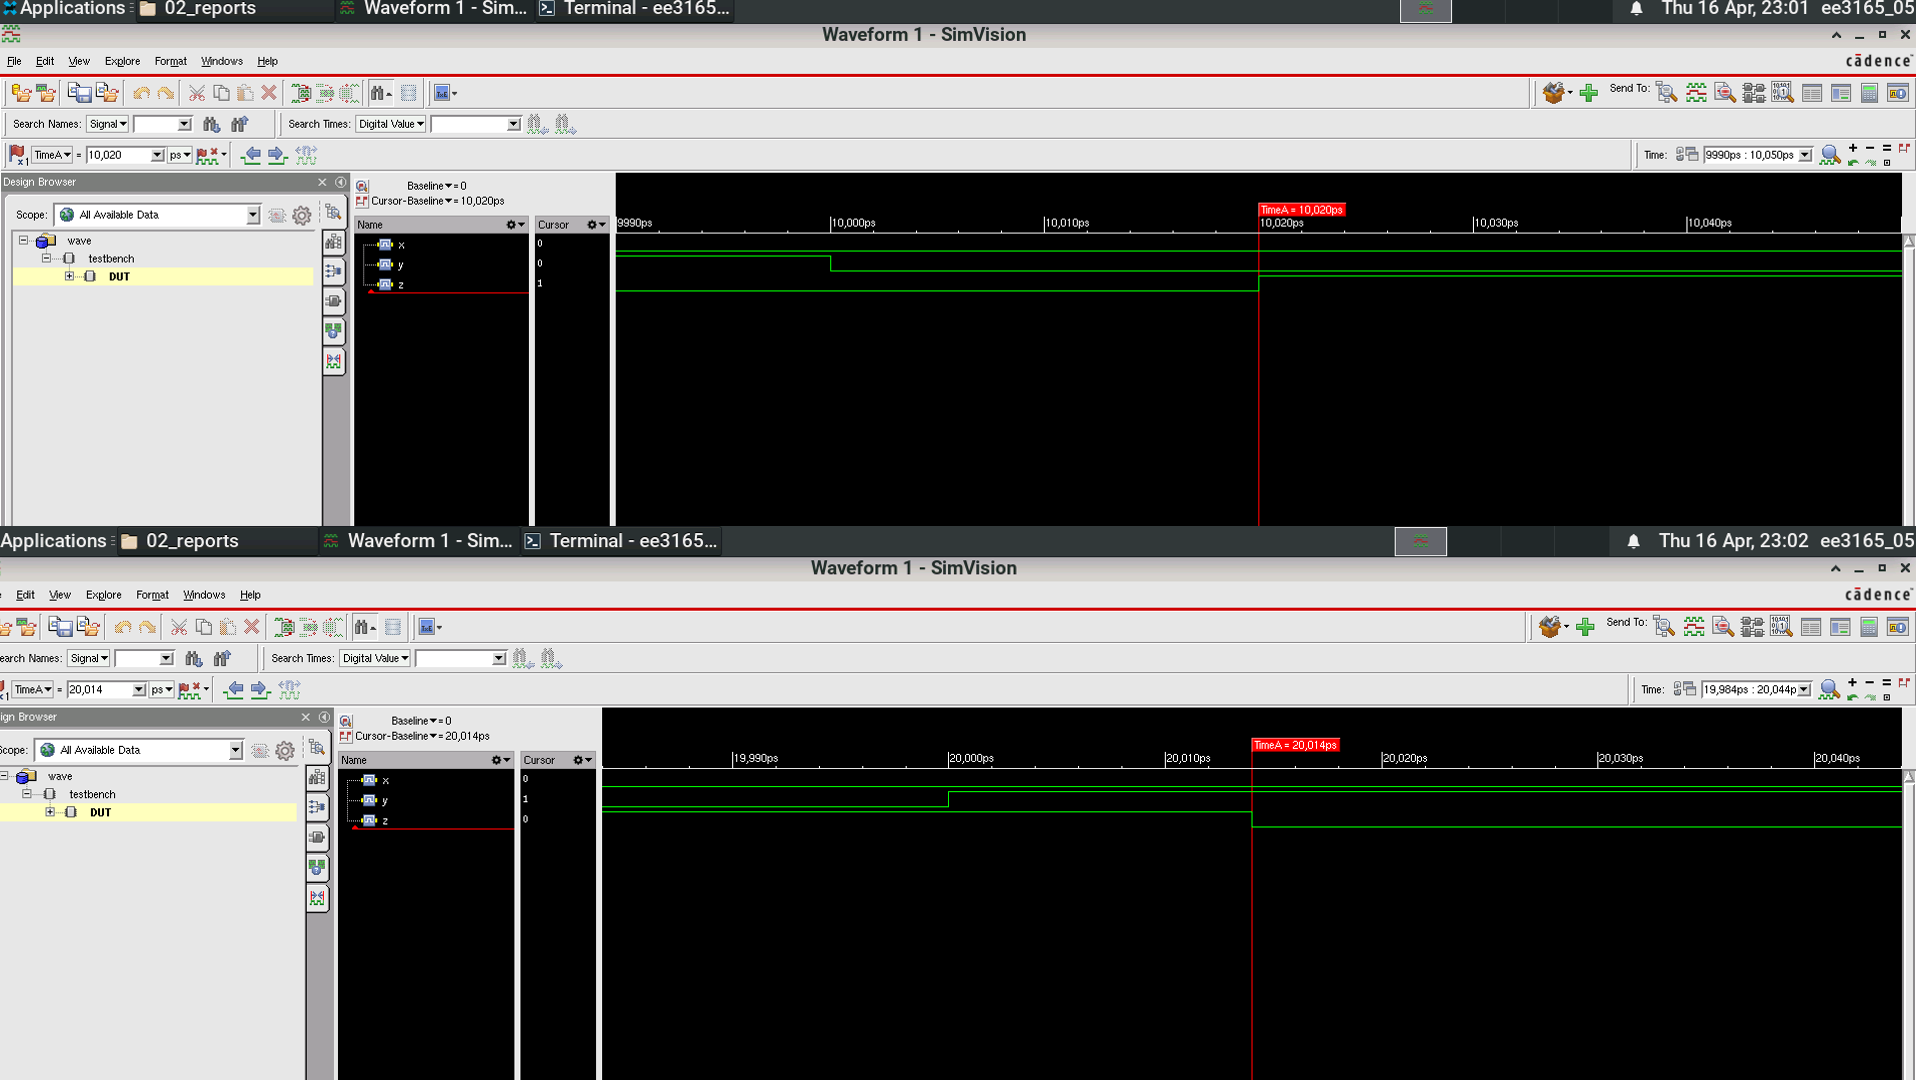
\includegraphics[width=\textwidth]{figures/exp1_nor2_lvt_slow_1v0.png}
        \caption{Góc LVT Slow (slow\_vdd1v0)}
        \label{fig:nor2_lvt_slow_1v0}
    \end{subfigure}
    \caption{Dạng sóng đo độ trễ cổng NOR2 sử dụng thư viện LVT tại 1.0V. Hình ảnh đại diện cho đường dẫn A$\rightarrow$Y.}
    \label{fig:nor2_lvt_comparison_1v0}
\end{figure}

\textbf{Nhận xét đặc tính LVT tại 1.0V:}
\begin{itemize}
    \item \textbf{Duy trì khả năng nạp tụ ở điện áp thấp:} Mặc dù hoạt động ở điện áp nguồn bị suy giảm, thư viện LVT với rào cản điện áp ngưỡng nhỏ giúp dòng điện dễ dàng đi qua mạng PMOS nối tiếp. Độ trễ sườn lên tại góc chậm nhất đã giảm gần một nửa, từ $0.036ns$ (của HVT) xuống chỉ còn $0.020ns$. Điều này biến LVT thành giải pháp hoàn hảo để đảm bảo thời gian thiết lập trong các hệ thống ưu tiên tiết kiệm năng lượng.
    \item \textbf{Sự gia tăng công suất rò rỉ:} Để có được tốc độ phản hồi nhanh chóng, linh kiện LVT luôn có dòng điện rò rỉ chạy qua kênh dẫn ngay cả ở trạng thái tắt. Tổng công suất của góc chậm nhất đạt $7.82 \times 10^{-9}W$, cao hơn một cách rõ rệt so với thư viện HVT.
\end{itemize}

\textbf{Khảo sát đặc tính LVT tại điều kiện 1.2V (Điện áp danh định):}

\begin{figure}[H]
    \centering
    \begin{subfigure}[b]{0.48\textwidth}
        \centering
        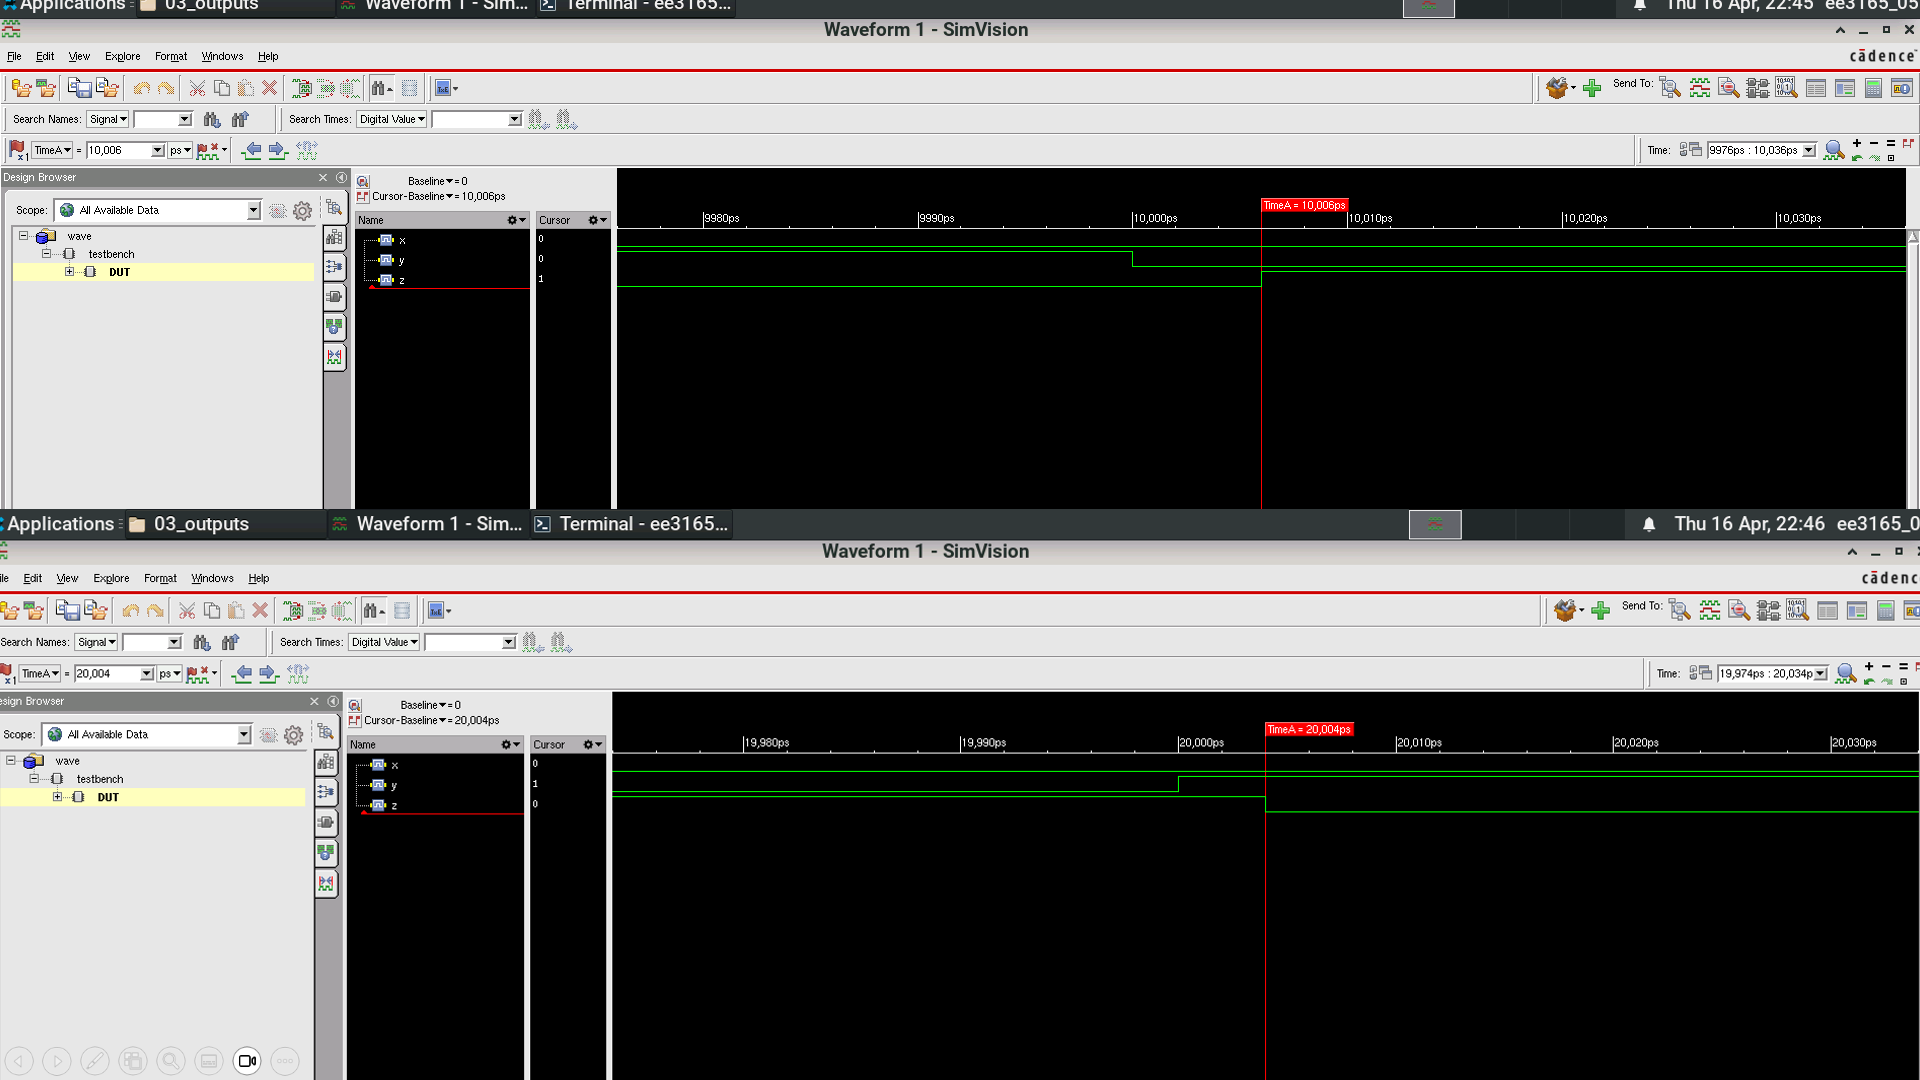
\includegraphics[width=\textwidth]{figures/exp1_nor2_lvt_fast_1v2.png}
        \caption{Góc LVT Fast (fast\_vdd1v2)}
        \label{fig:nor2_lvt_fast_1v2}
    \end{subfigure}
    \hfill
    \begin{subfigure}[b]{0.48\textwidth}
        \centering
        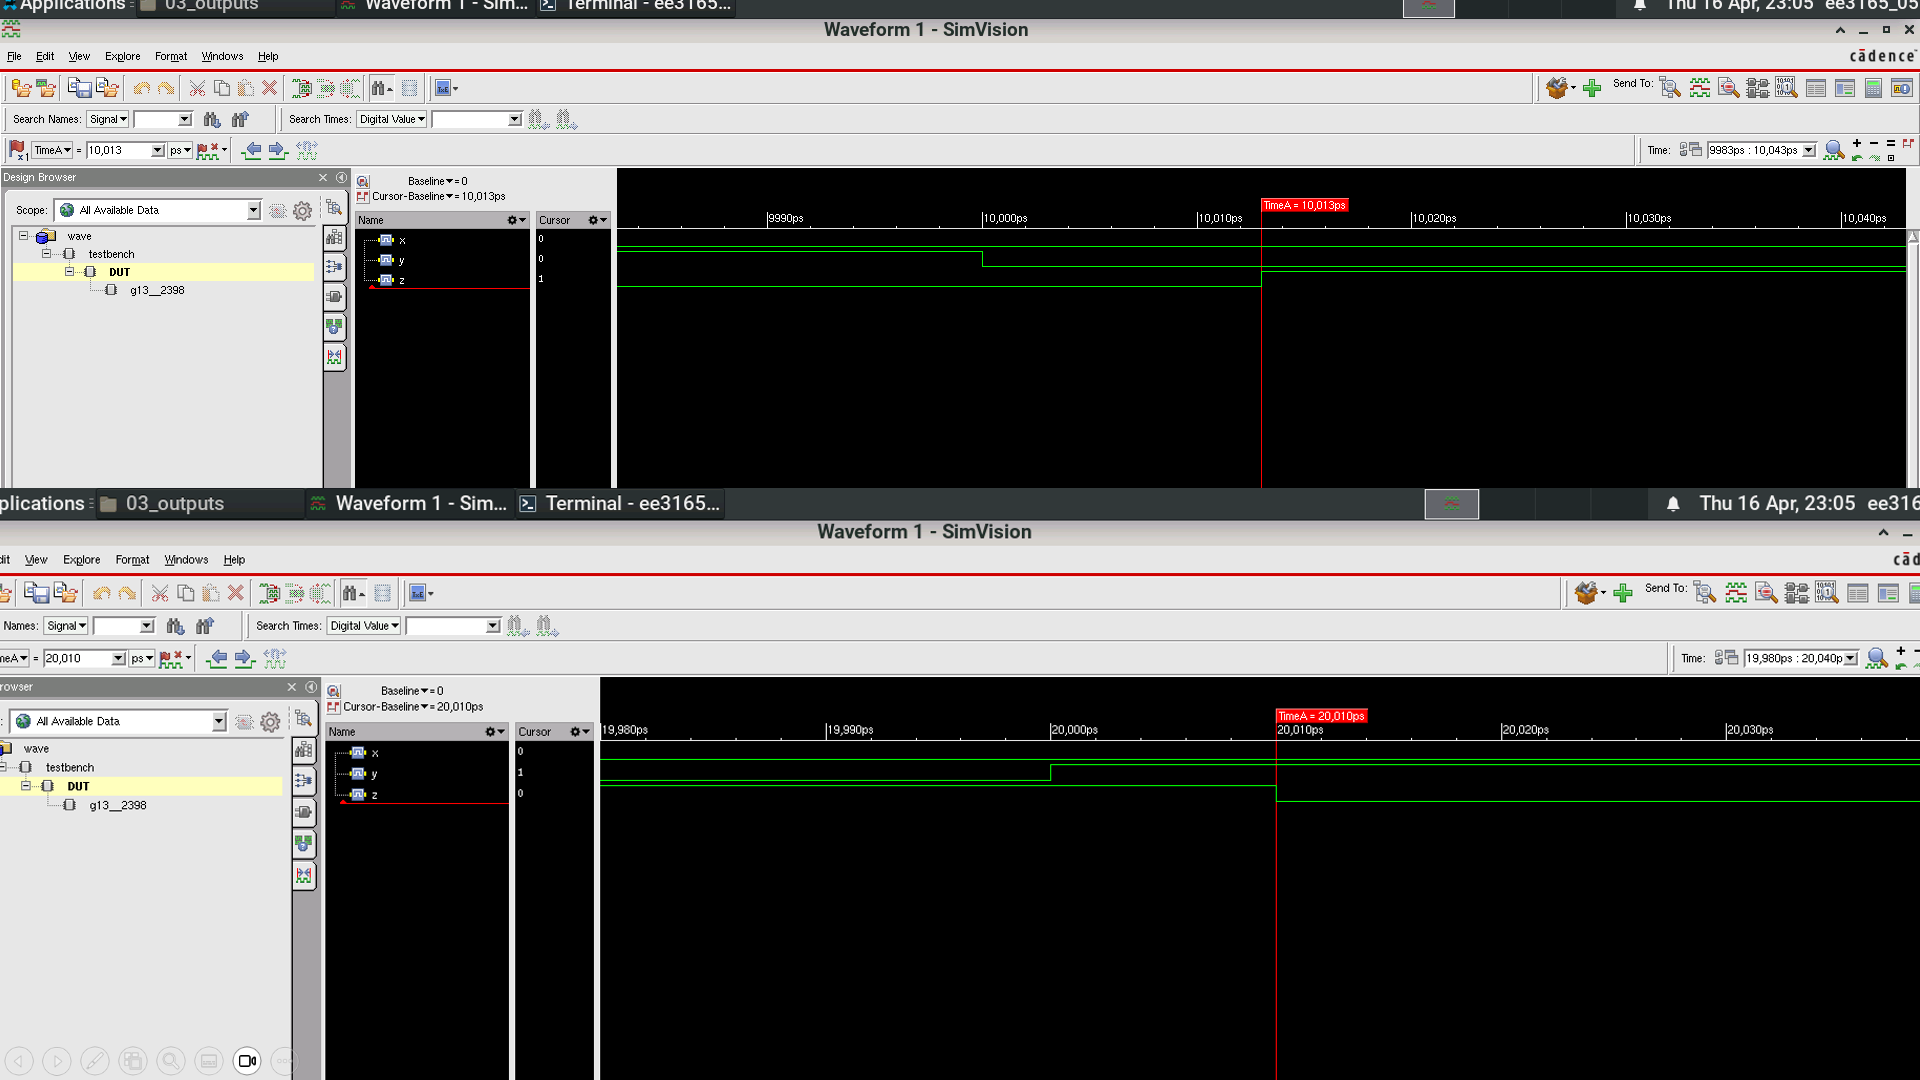
\includegraphics[width=\textwidth]{figures/exp1_nor2_lvt_slow_1v2.png}
        \caption{Góc LVT Slow (slow\_vdd1v2)}
        \label{fig:nor2_lvt_slow_1v2}
    \end{subfigure}
    \caption{Dạng sóng đo độ trễ cổng NOR2 sử dụng thư viện LVT tại 1.2V. Hình ảnh đại diện cho đường dẫn A$\rightarrow$Y.}
    \label{fig:nor2_lvt_comparison_1v2}
\end{figure}

\textbf{Nhận xét đặc tính LVT tại 1.2V:}
\begin{itemize}
    \item \textbf{Hiệu năng cực hạn:} Tại góc vận hành lý tưởng nhất, sự kết hợp giữa điện áp cao và thư viện tốc độ nhanh giúp độ trễ sườn lên của chân B chỉ mất $0.004ns$. Mạch đạt trạng thái bão hòa dòng điện tối đa, tạo ra các sườn tín hiệu cực kỳ dốc.
    \item \textbf{Giới hạn nhiệt độ và công suất:} Góc cấu hình này cũng đồng thời là điều kiện tiêu tốn năng lượng khổng lồ nhất của cổng NOR2, chạm mốc $2.03 \times 10^{-8}W$. Sự gia tăng của cả năng lượng chuyển mạch và năng lượng tĩnh bắt buộc quá trình tổng hợp thiết kế phải áp dụng cell này một cách thật sự hạn chế để tránh vi phạm các rào cản về nhiệt độ cho lõi vi mạch.
\end{itemize}

\paragraph{C. Kết luận} 
Qua phân tích sâu về đặc tính thời gian và công suất, có thể thấy cổng NOR2 mang một điểm nghẽn vật lý cố hữu ở mạng kéo lên do hai transistor PMOS mắc nối tiếp. Để khắc phục độ trễ sườn lên thường xuyên lớn hơn sườn xuống này, thư viện LVT là một công cụ đắc lực giúp kéo giảm thời gian trễ một cách triệt để. Tuy nhiên, sự biến thiên cố định của diện tích ($1.026 \mu m^2$) trên mọi góc đo khẳng định rằng, việc tối ưu hóa thiết kế luôn là một bài toán cân đối không ngừng giữa Tốc độ cực đại và Công suất tiêu thụ tối thiểu.

\newpage
\subsubsection{MUX}
\begin{lstlisting}[style={prettyverilog}, caption={\texttt{code thiết kế MUX}}]
`timescale 1ns/1ps
module mux(
    input logic d0, d1, s,
      output logic y);
    assign y = s ? d1 : d0;
endmodule
\end{lstlisting}
\begin{lstlisting}[style={prettyverilog}, caption={\texttt{code testbench MUX}}]
`timescale 1ns/1ps
module tb_mux;
    logic D0, D1, S;
    logic Y;
    mux2 DUT(.d0(D0), .d1(D1), .s(S), .y(Y));
    initial begin
        $dumpfile("mux_wave.vcd");
        $dumpvars(0, tb_mux);
        D0 = 0; D1 = 0; S = 1; #10;
        D0 = 0; D1 = 1; S = 1; #10;
        D0 = 0; D1 = 0; S = 1; #10;
        D0 = 0; D1 = 0; S = 0; #10;
        D0 = 1; D1 = 0; S = 0; #10;
        D0 = 0; D1 = 1; S = 0; #10;
        D0 = 0; D1 = 1; S = 1; #10;
        D0 = 0; D1 = 1; S = 0; #10;
        $finish;
    end
endmodule
\end{lstlisting}

Trước hết, để tổng quan về linh kiện, Hình \ref{fig:exp1_mux} trình bày ký hiệu logic cơ bản của bộ dồn kênh MUX 2:1. Linh kiện này cho phép chọn một trong hai tín hiệu dữ liệu ngõ vào (\texttt{D0} hoặc \texttt{D1}) để đưa ra ngõ ra \texttt{Y} dựa trên tín hiệu điều khiển \texttt{S}. Phương trình đại số Boole của thiết kế là $Y = \overline{S} \cdot D0 + S \cdot D1$.

\begin{figure}[H]
    \centering
    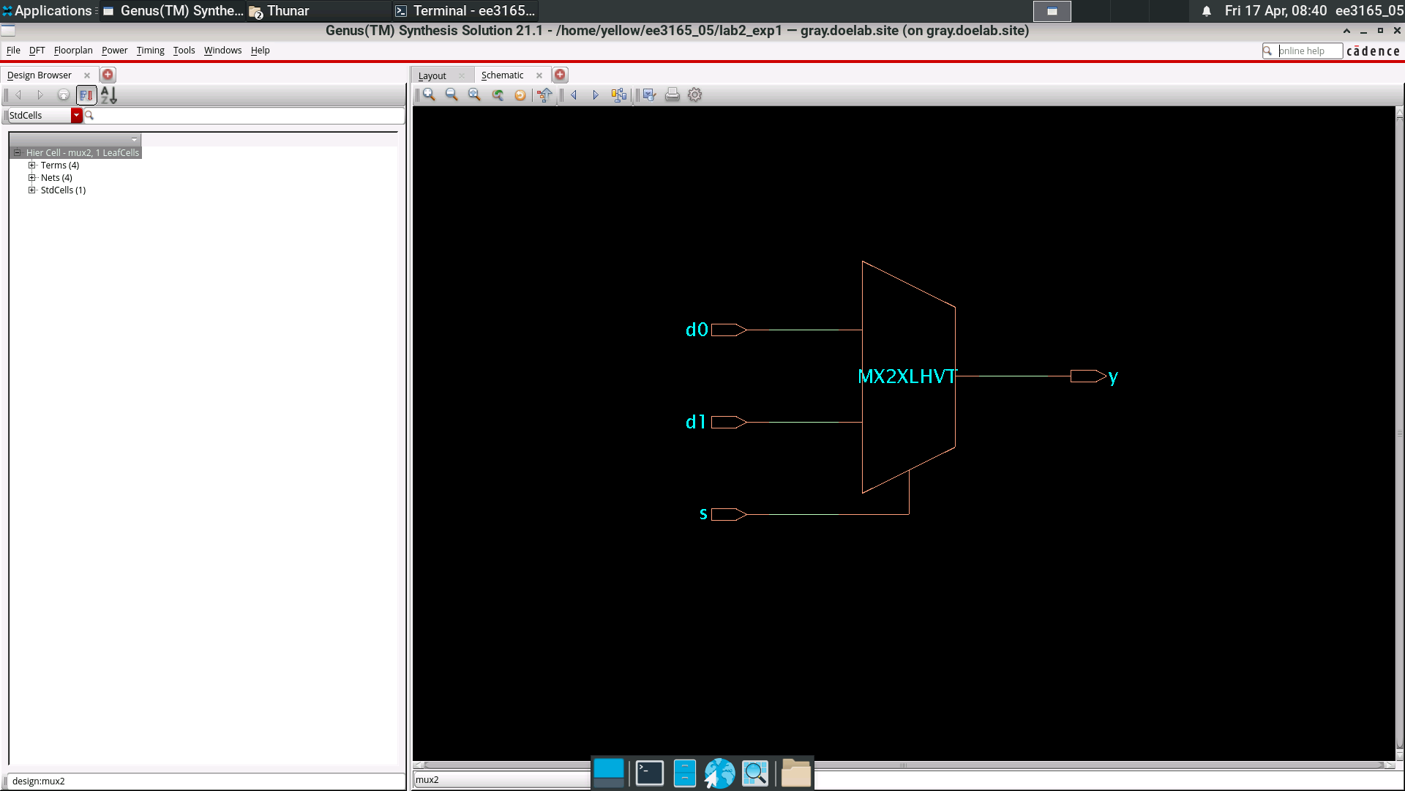
\includegraphics[width=0.6\textwidth]{figures/exp1_mux.png}
    \caption{Ký hiệu logic và đặc tính cơ bản của cổng MUX 2:1.}
    \label{fig:exp1_mux}
\end{figure}

Sau khi viết mã RTL, thiết kế được đưa vào công cụ Genus để thực hiện quá trình tổng hợp. Hình \ref{fig:exp1_mux_mapped} minh họa sơ đồ mức cổng của MUX sau khi được ánh xạ vào thư viện công nghệ 45nm.

\begin{figure}[H]
    \centering
    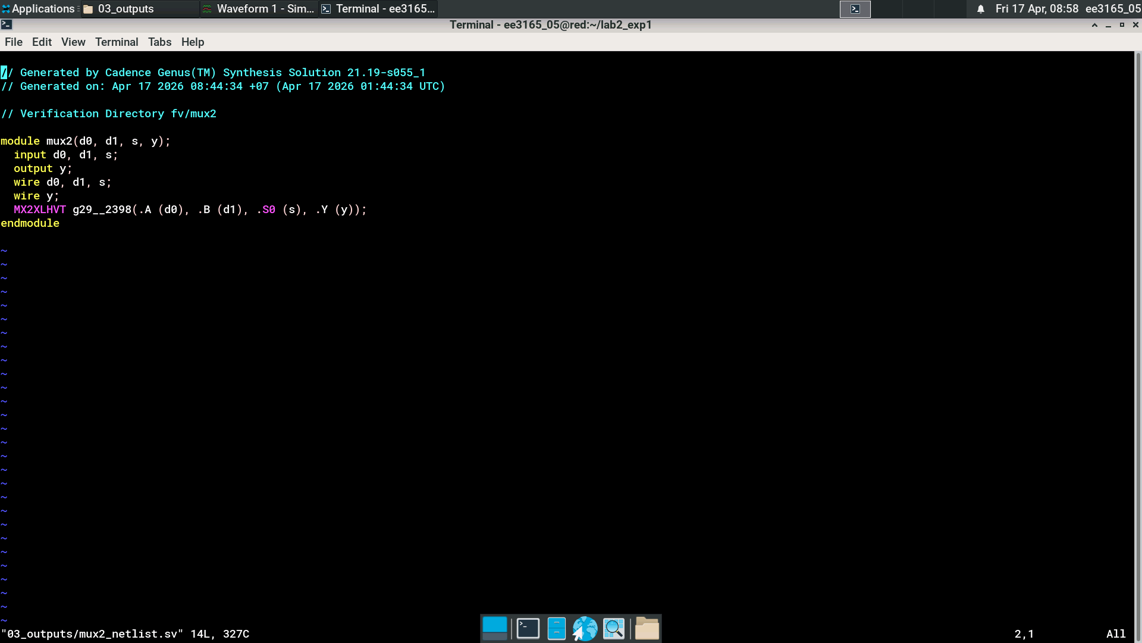
\includegraphics[width=0.7\textwidth]{figures/exp1_mux_mapped.png}
    \caption{Sơ đồ mức cổng của thiết kế MUX trên giao diện Genus.}
    \label{fig:exp1_mux_mapped}
\end{figure}

Nhóm tiếp tục thực hiện khảo sát đặc tính của cổng MUX trên cả hai loại thư viện: High Threshold Voltage (HVT) và Low Threshold Voltage (LVT). Do MUX có 3 ngõ vào, quá trình đo đạc độ trễ sẽ được đánh giá trên cả 3 đường dẫn tín hiệu: từ dữ liệu đến ngõ ra (\texttt{D0$\rightarrow$Y}, \texttt{D1$\rightarrow$Y}) và từ chân lựa chọn đến ngõ ra (\texttt{S$\rightarrow$Y}).

\paragraph{A. Thư viện High Threshold Voltage (HVT)}
Đặc tính của các cell HVT là dòng rò thấp nhưng độ trễ lớn hơn. Kết quả mô phỏng 8 góc quy trình được tổng hợp trong bảng dưới đây:

\begin{table}[H]
\centering
\renewcommand{\arraystretch}{1.3}
\resizebox{\textwidth}{!}{
\begin{tabular}{|l|c|c|c|c|c|c|c|c|}
\hline
 
\multirow{2}{*}{\textbf{Library Name}} 
& \multirow{2}{*}{\textbf{Total Area}} 
& \multirow{2}{*}{\textbf{Total Power}} 
 
& \multicolumn{2}{c|}{\textbf{Delay D0$\rightarrow$Y}}
& \multicolumn{2}{c|}{\textbf{Delay D1$\rightarrow$Y}} 
& \multicolumn{2}{c|}{\textbf{Delay S$\rightarrow$Y}} \\
 
\cline{4-9}
 
& & 
& \textbf{Rise (ns)} & \textbf{Fall (ns)}
& \textbf{Rise (ns)} & \textbf{Fall (ns)}
& \textbf{Rise (ns)} & \textbf{Fall (ns)} \\
 
\hline
 
% ----------- KHỐI HVT ----------------
 
fast\_vdd1v0\_basicCells\_hvt 
& 2.394 & 3.65866e-08 
& 0.034 & 0.036
& 0.034 & 0.037 
& 0.038 & 0.040 \\ \hline
 
fast\_vdd1v2\_basicCells\_hvt 
& 2.394 & 5.47016e-08 
& 0.024 & 0.027
& 0.024 & 0.027 
& 0.027 & 0.029 \\ \hline
 
slow\_vdd1v0\_basicCells\_hvt 
& 2.394 & 2.39599e-08 
& 0.203 & 0.126
& 0.202 & 0.130 
& 0.199 & 0.152 \\ \hline
 
slow\_vdd1v2\_basicCells\_hvt 
& 2.394 & 3.62320e-08 
& 0.088 & 0.064
& 0.087 & 0.065 
& 0.089 & 0.074 \\ \hline
 
\end{tabular}
}

\caption{Tổng hợp thông số Diện tích, Công suất và Độ trễ của cổng MUX (HVT).}
\label{tab:exp1_mux_hvt_params}

\end{table}

Dưới đây là sự so sánh dạng sóng mô phỏng của cổng MUX tại hai góc cực đoan ở cùng mức điện áp 1.0V.

\begin{figure}[H]
    \centering
    \begin{subfigure}[b]{0.48\textwidth}
        \centering
        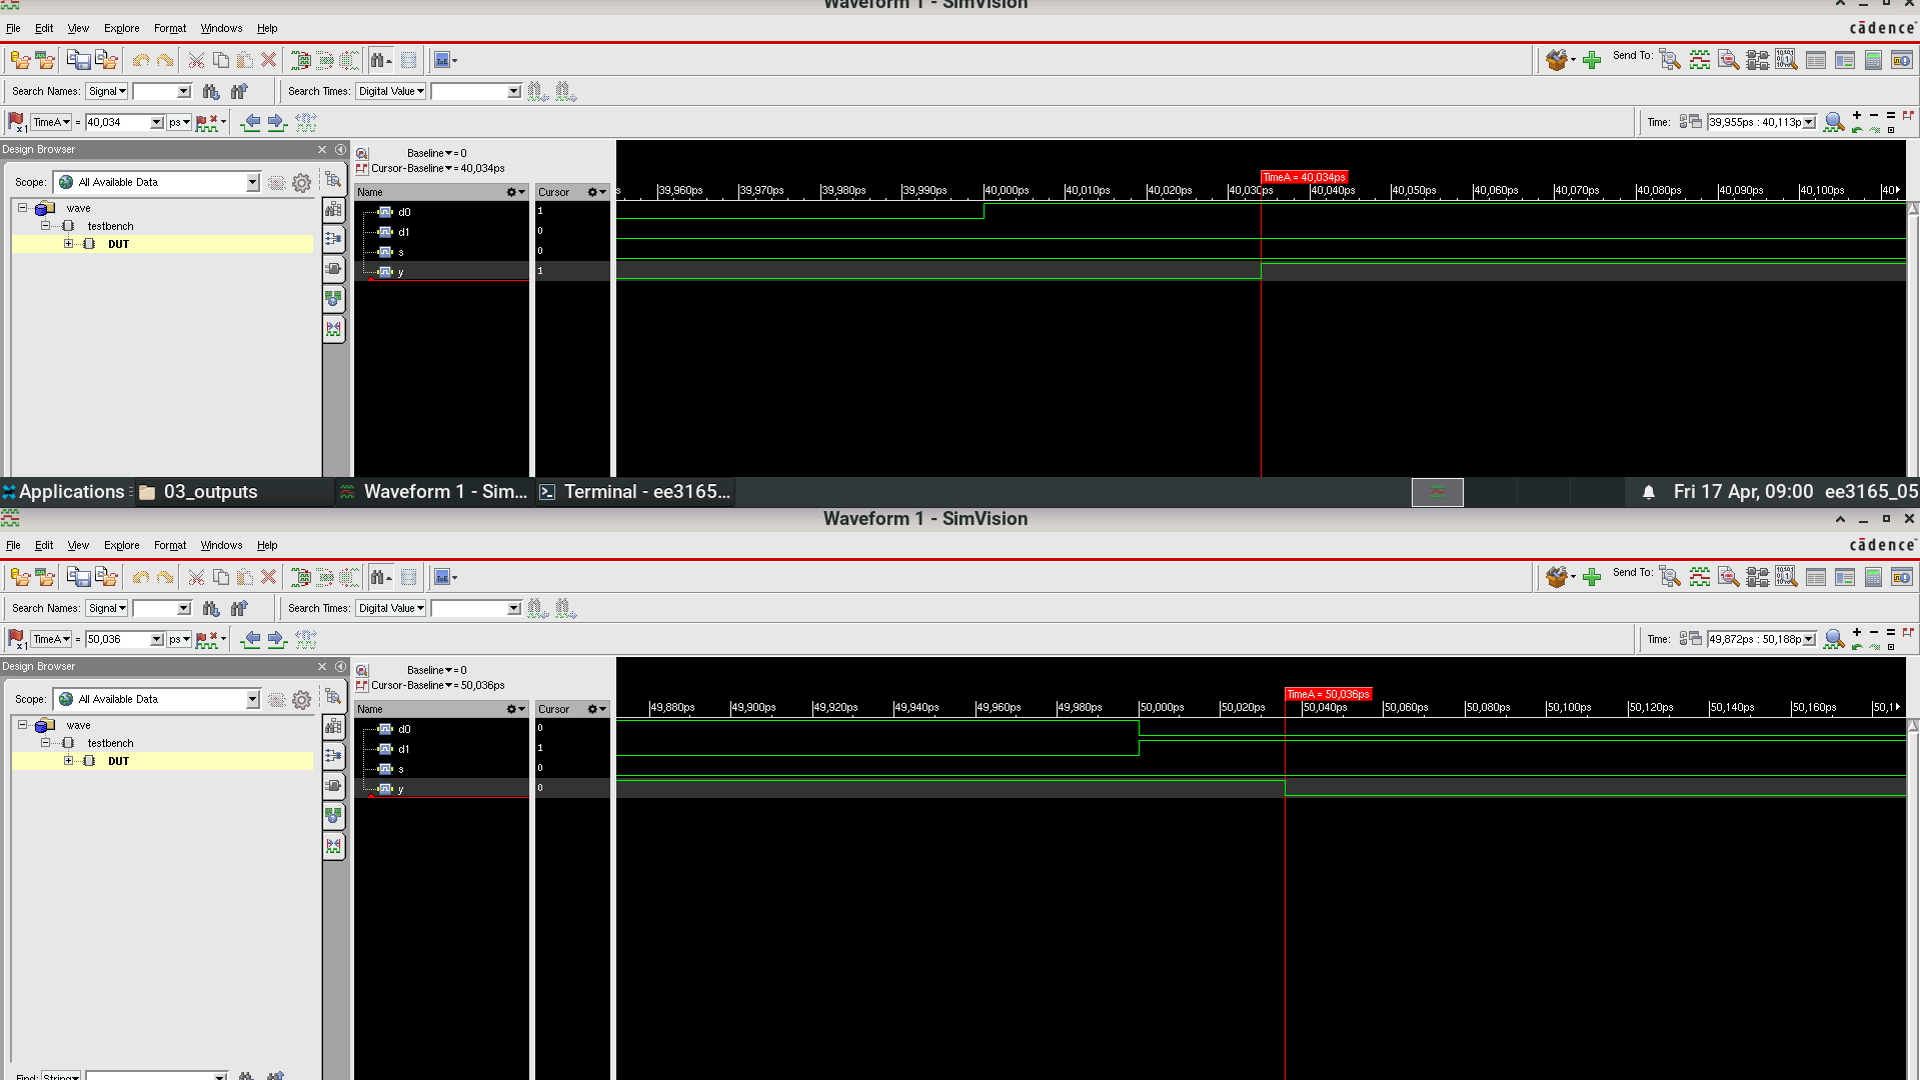
\includegraphics[width=\textwidth]{figures/exp1_mux_hvt_fast_1v0.png}
        \caption{Góc HVT Fast (fast\_vdd1v0)}
    \end{subfigure}
    \hfill
    \begin{subfigure}[b]{0.48\textwidth}
        \centering
        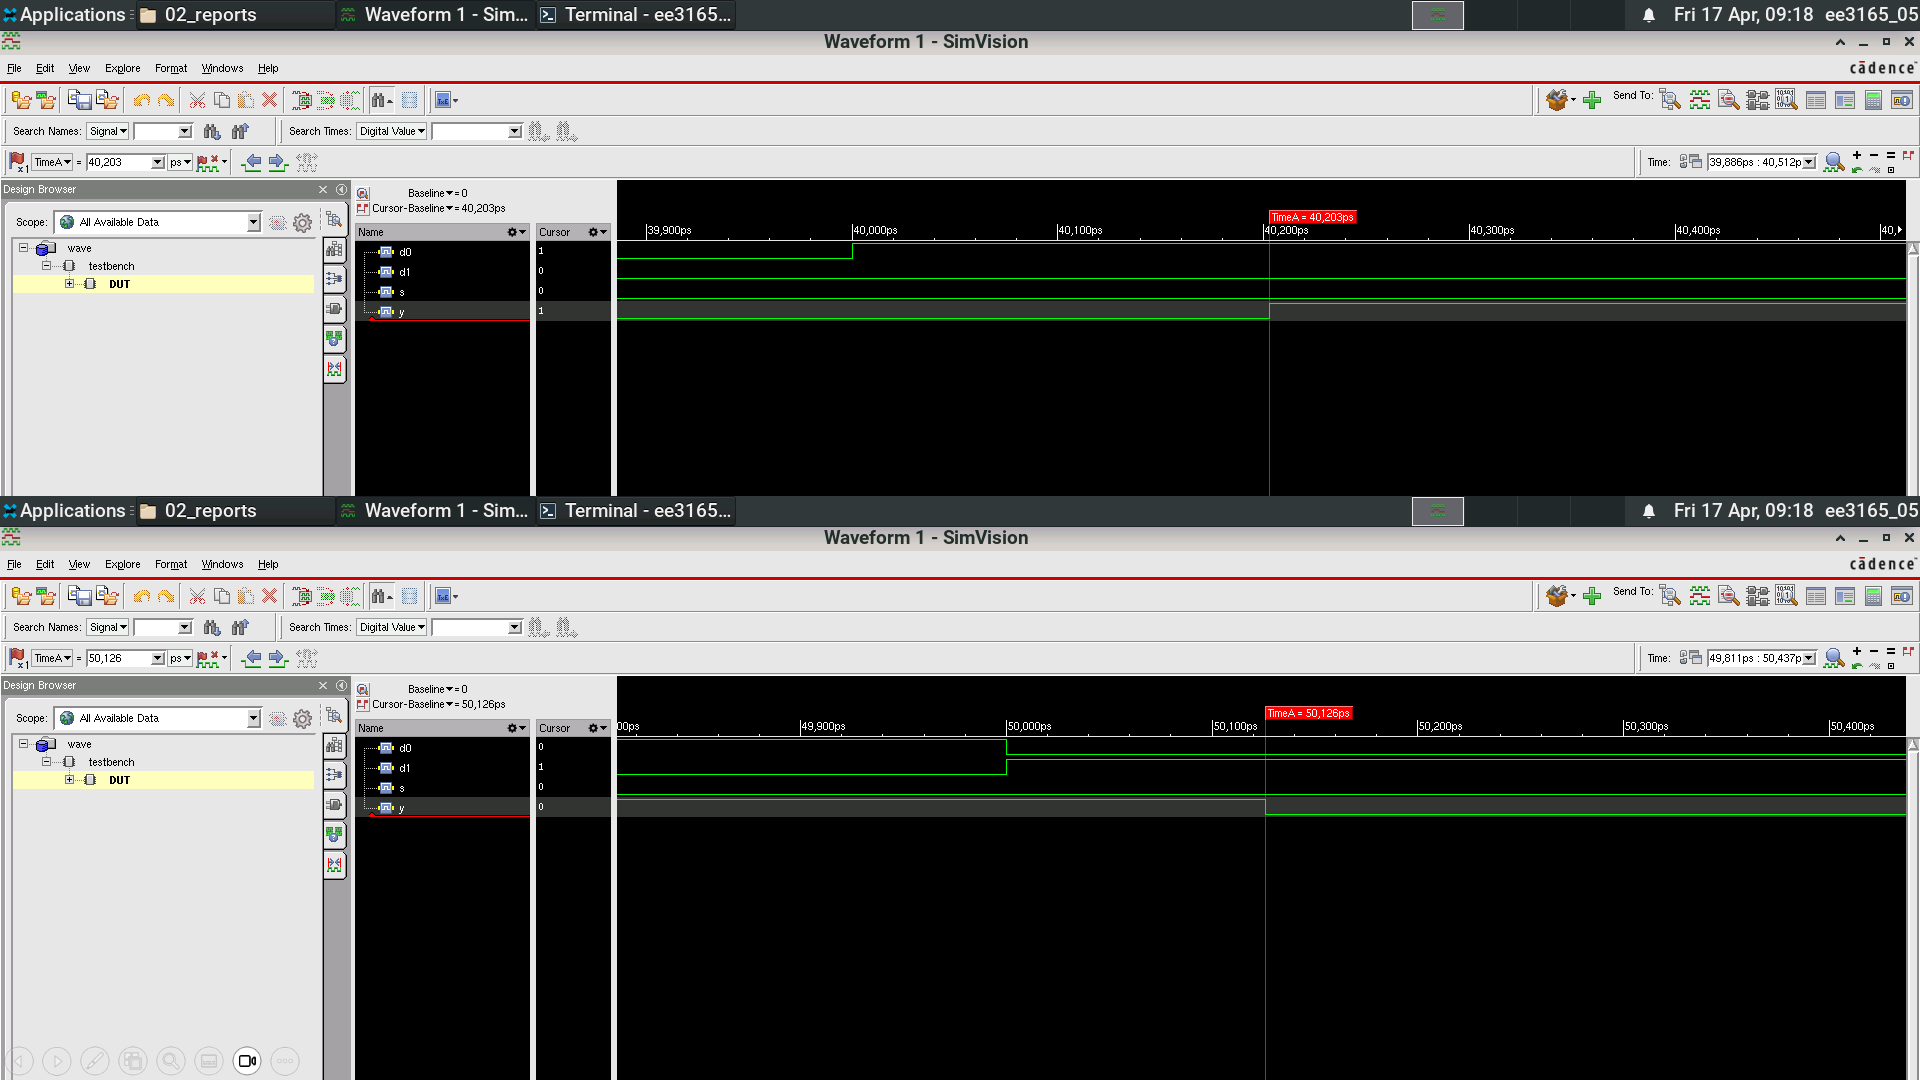
\includegraphics[width=\textwidth]{figures/exp1_mux_hvt_slow_1v0.png}
        \caption{Góc HVT Slow (slow\_vdd1v0)}
    \end{subfigure}
    \caption{Dạng sóng đo độ trễ cổng MUX ở HVT (VDD = 1.0V). Hình ảnh đại diện cho đường dẫn D0$\rightarrow$Y.}
    \label{fig:mux_hvt_comparison_1v0}
\end{figure}

\textbf{Nhận xét (HVT - 1.0V):} Dựa trên số liệu đo đạc, cổng MUX thể hiện độ phức tạp cao hơn hẳn các cổng logic cơ bản:
\begin{itemize}
    \item \textbf{Suy giảm hiệu năng nghiêm trọng do thiếu áp:} Ở 1.0V, dòng bão hòa của cell HVT suy yếu cực độ. Tại góc chậm nhất, độ trễ sườn lên của ngõ \texttt{D0} tăng vọt lên mức $0.203ns$, lớn hơn gấp nhiều lần so với các cổng NAND hay NOR. Điều này biến MUX thành điểm nghẽn thời gian lớn trong hệ thống.
    \item \textbf{Sự khác biệt giữa các đường dẫn tín hiệu:} Bảng số liệu cho thấy độ trễ từ chân chọn \texttt{S} ra \texttt{Y} thường lớn hơn so với từ \texttt{D0}/\texttt{D1} ra \texttt{Y} (ví dụ sườn xuống của \texttt{S} mất $0.152ns$ so với $0.126ns$ của \texttt{D0}). Nguyên nhân là do tín hiệu \texttt{S} phải đi qua nhiều tầng logic đảo và cổng truyền nội bộ hơn để điều khiển các nhánh dữ liệu. Đường \texttt{S$\rightarrow$Y} thường xuyên đóng vai trò là đường dẫn tới hạn.
    \item \textbf{Tối ưu hóa năng lượng tĩnh:} Để bù đắp cho tốc độ chậm, HVT tại góc chậm nhất cung cấp khả năng tiết kiệm điện năng ấn tượng với tổng công suất chỉ $2.39 \times 10^{-8}W$.
\end{itemize}

\vspace{1cm}

Dưới đây là kết quả mô phỏng tại điện áp danh định 1.2V cho thư viện HVT.

\begin{figure}[H]
    \centering
    \begin{subfigure}[b]{0.48\textwidth}
        \centering
        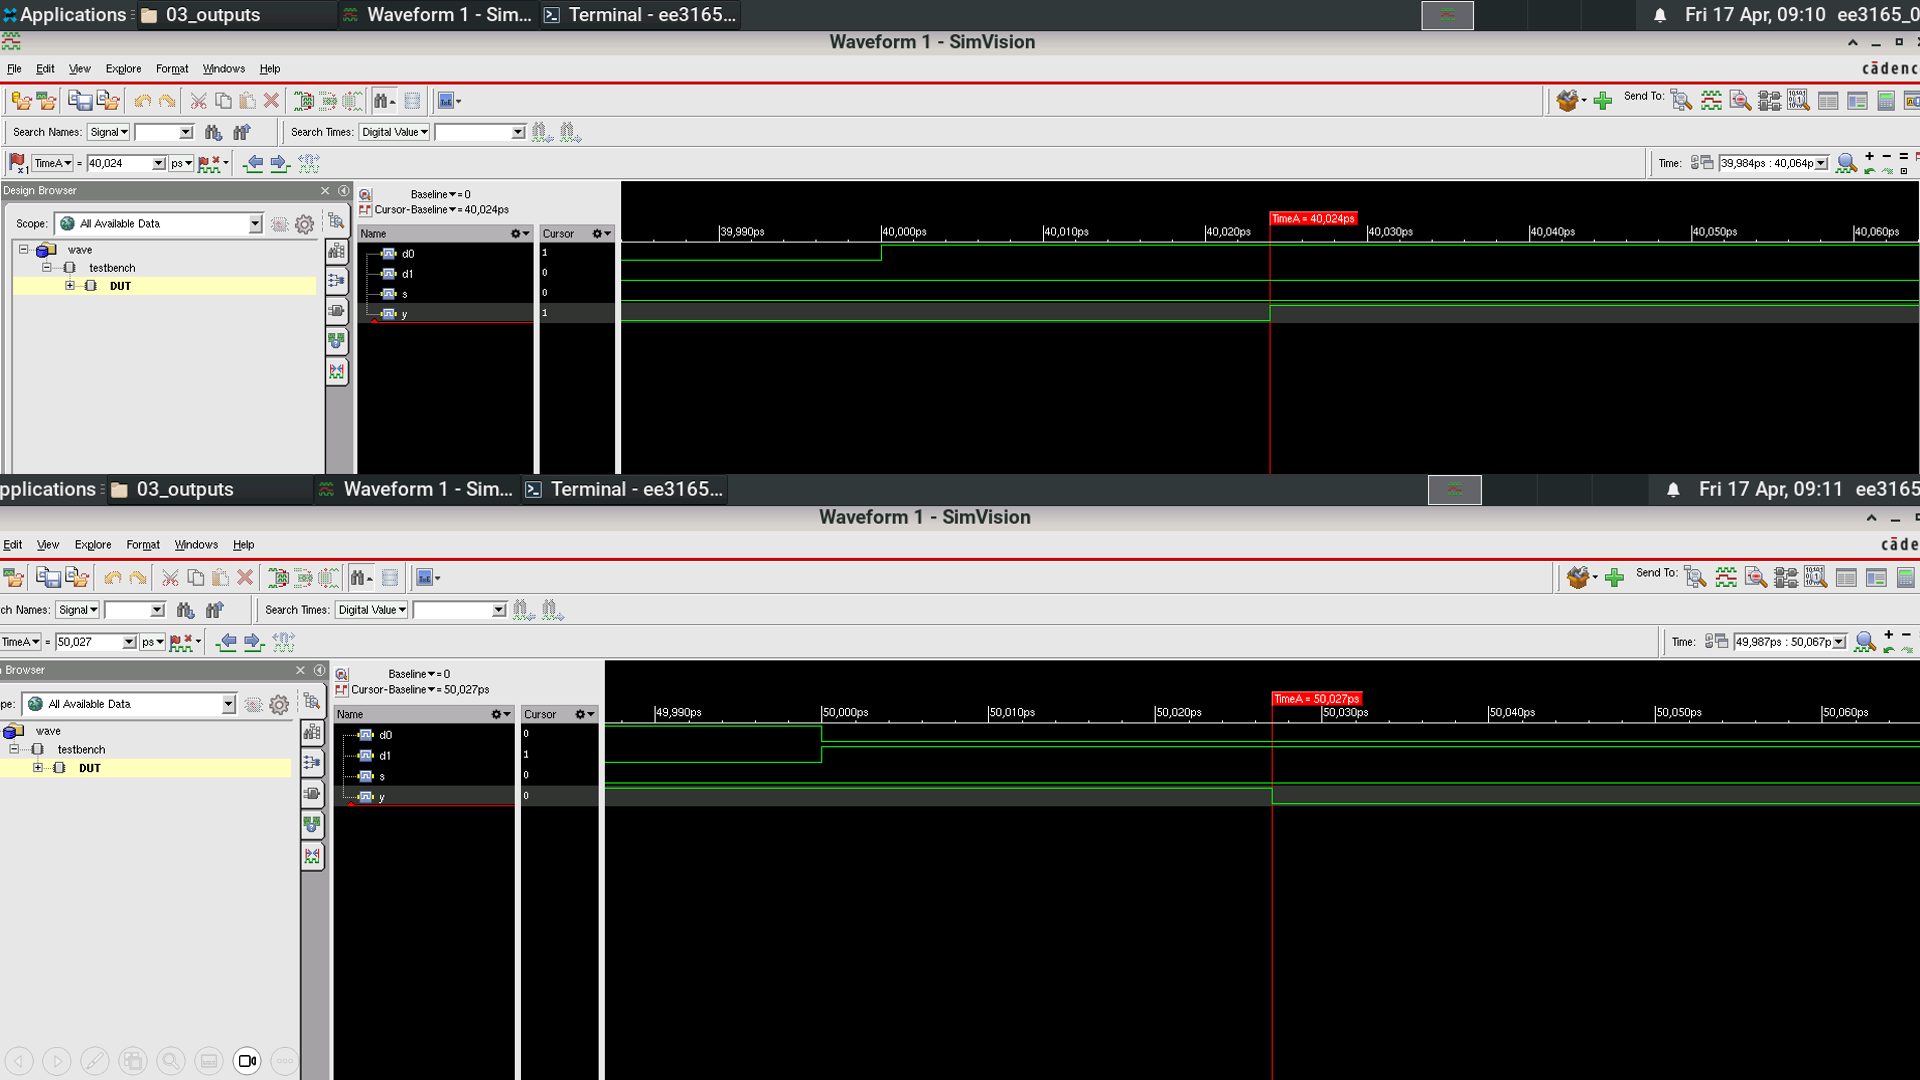
\includegraphics[width=\textwidth]{figures/exp1_mux_hvt_fast_1v2.png}
        \caption{Góc HVT Fast (fast\_vdd1v2)}
    \end{subfigure}
    \hfill
    \begin{subfigure}[b]{0.48\textwidth}
        \centering
        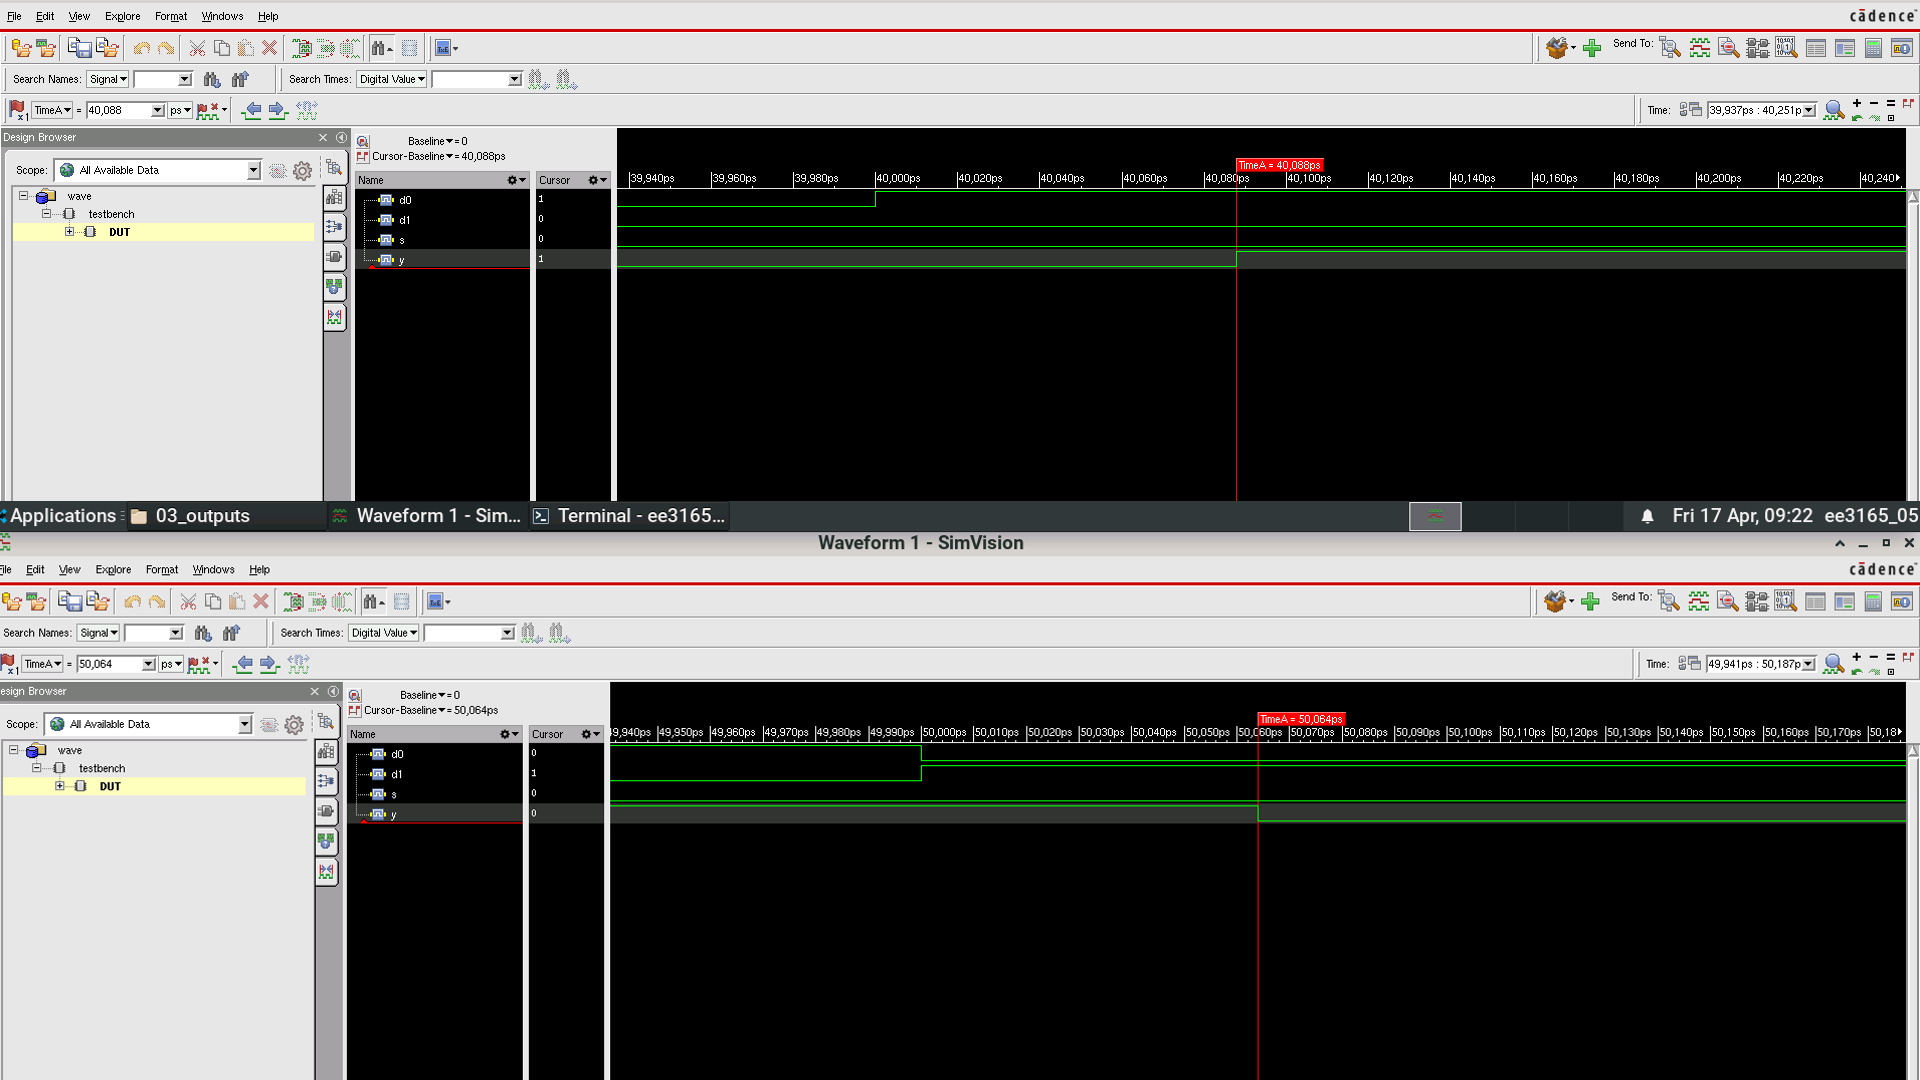
\includegraphics[width=\textwidth]{figures/exp1_mux_hvt_slow_1v2.png}
        \caption{Góc HVT Slow (slow\_vdd1v2)}
    \end{subfigure}
    \caption{Dạng sóng đo độ trễ cổng MUX ở HVT (VDD = 1.2V). Hình ảnh đại diện cho đường dẫn D0$\rightarrow$Y.}
    \label{fig:mux_hvt_comparison_1v2}
\end{figure}

\textbf{Nhận xét (HVT - 1.2V):} 
\begin{itemize}
    \item \textbf{Phục hồi tốc độ chuyển mạch:} Việc trả lại mức điện áp 1.2V giúp các transistor nạp xả tụ linh hoạt hơn. Ở góc nhanh nhất, độ trễ trên mọi đường dẫn đều giảm xuống dưới $0.030ns$, đáp ứng tốt các chuẩn thời gian thiết lập cơ bản.
    \item \textbf{Đánh đổi công suất:} Cùng với việc tăng tốc độ, điện áp cao đẩy tổng công suất tiêu thụ tại góc nhanh nhất lên mức $5.47 \times 10^{-8}W$.
\end{itemize}

\paragraph{B. Thư viện Low Threshold Voltage (LVT)}
Các cell LVT cho tốc độ chuyển mạch nhanh hơn nhờ điện áp ngưỡng thấp, đổi lại công suất tiêu thụ tĩnh cao hơn do dòng rò dưới ngưỡng.

\begin{table}[H]
\centering
\renewcommand{\arraystretch}{1.3}
\resizebox{\textwidth}{!}{
\begin{tabular}{|l|c|c|c|c|c|c|c|c|}
\hline
 
\multirow{2}{*}{\textbf{Library Name}} 
& \multirow{2}{*}{\textbf{Total Area}} 
& \multirow{2}{*}{\textbf{Total Power}} 
 
& \multicolumn{2}{c|}{\textbf{Delay D0$\rightarrow$Y}}
& \multicolumn{2}{c|}{\textbf{Delay D1$\rightarrow$Y}} 
& \multicolumn{2}{c|}{\textbf{Delay S$\rightarrow$Y}} \\
 
\cline{4-9}
 
& & 
& \textbf{Rise (ns)} & \textbf{Fall (ns)}
& \textbf{Rise (ns)} & \textbf{Fall (ns)}
& \textbf{Rise (ns)} & \textbf{Fall (ns)} \\
 
\hline
 
% ----------- KHỐI LVT ----------------
 
fast\_vdd1v0\_basicCells\_lvt 
& 2.394 & 4.61418e-08 
& 0.020 & 0.022
& 0.019 & 0.022 
& 0.022 & 0.023 \\ \hline
 
fast\_vdd1v2\_basicCells\_lvt 
& 2.394 & 6.48883e-08 
& 0.015 & 0.018
& 0.015 & 0.018 
& 0.017 & 0.019 \\ \hline
 
slow\_vdd1v0\_basicCells\_lvt 
& 2.394 & 2.71963e-08 
& 0.077 & 0.066
& 0.076 & 0.068 
& 0.080 & 0.073 \\ \hline
 
slow\_vdd1v2\_basicCells\_lvt 
& 2.394 & 4.05591e-08 
& 0.048 & 0.044
& 0.048 & 0.045 
& 0.051 & 0.049 \\ \hline
 
\end{tabular}
}

\caption{Tổng hợp thông số Diện tích, Công suất và Độ trễ của MUX (LVT).}
\label{tab:exp1_mux_lvt_params}

\end{table}

\textbf{Khảo sát đặc tính LVT tại điều kiện 1.0V (Điện áp thấp):}

\begin{figure}[H]
    \centering
    \begin{subfigure}[b]{0.48\textwidth}
        \centering
        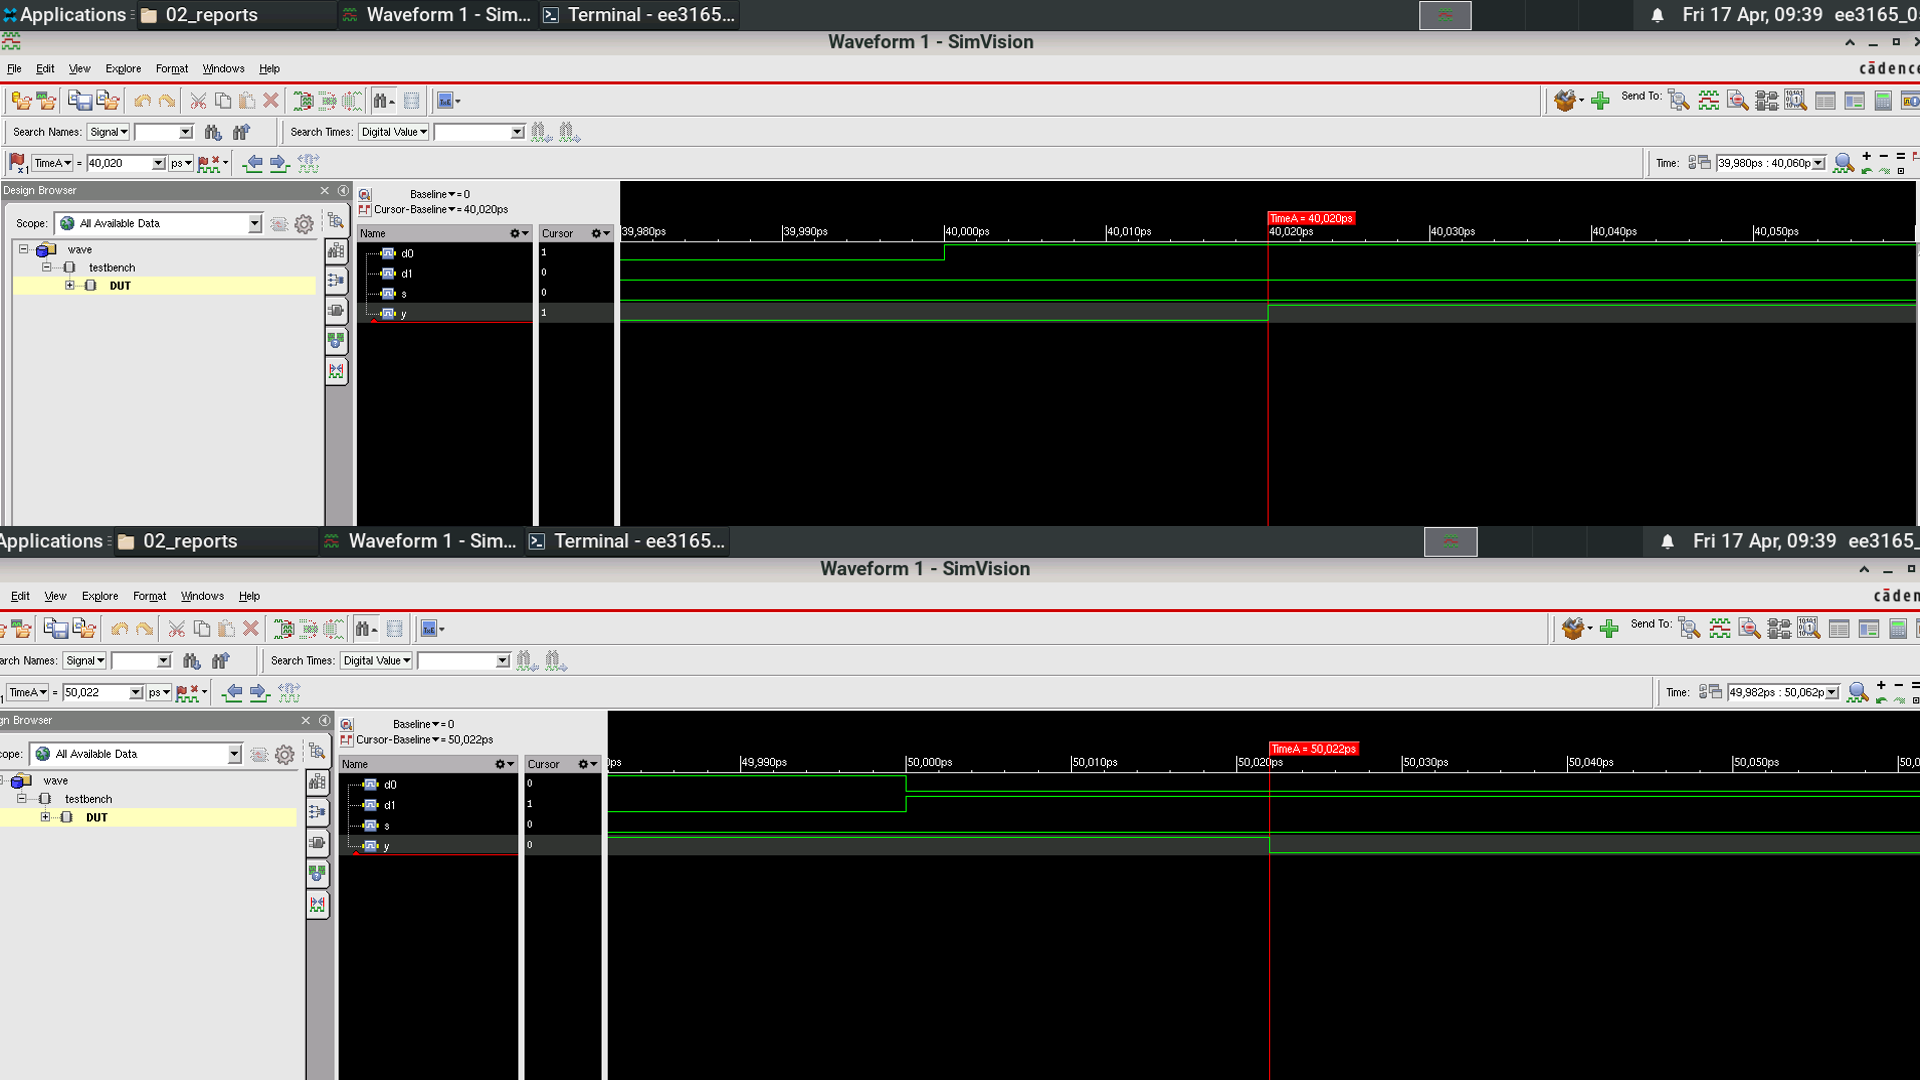
\includegraphics[width=\textwidth]{figures/exp1_mux_lvt_fast_1v0.png}
        \caption{Góc LVT Fast (fast\_vdd1v0)}
        \label{fig:mux_lvt_fast_1v0}
    \end{subfigure}
    \hfill
    \begin{subfigure}[b]{0.48\textwidth}
        \centering
        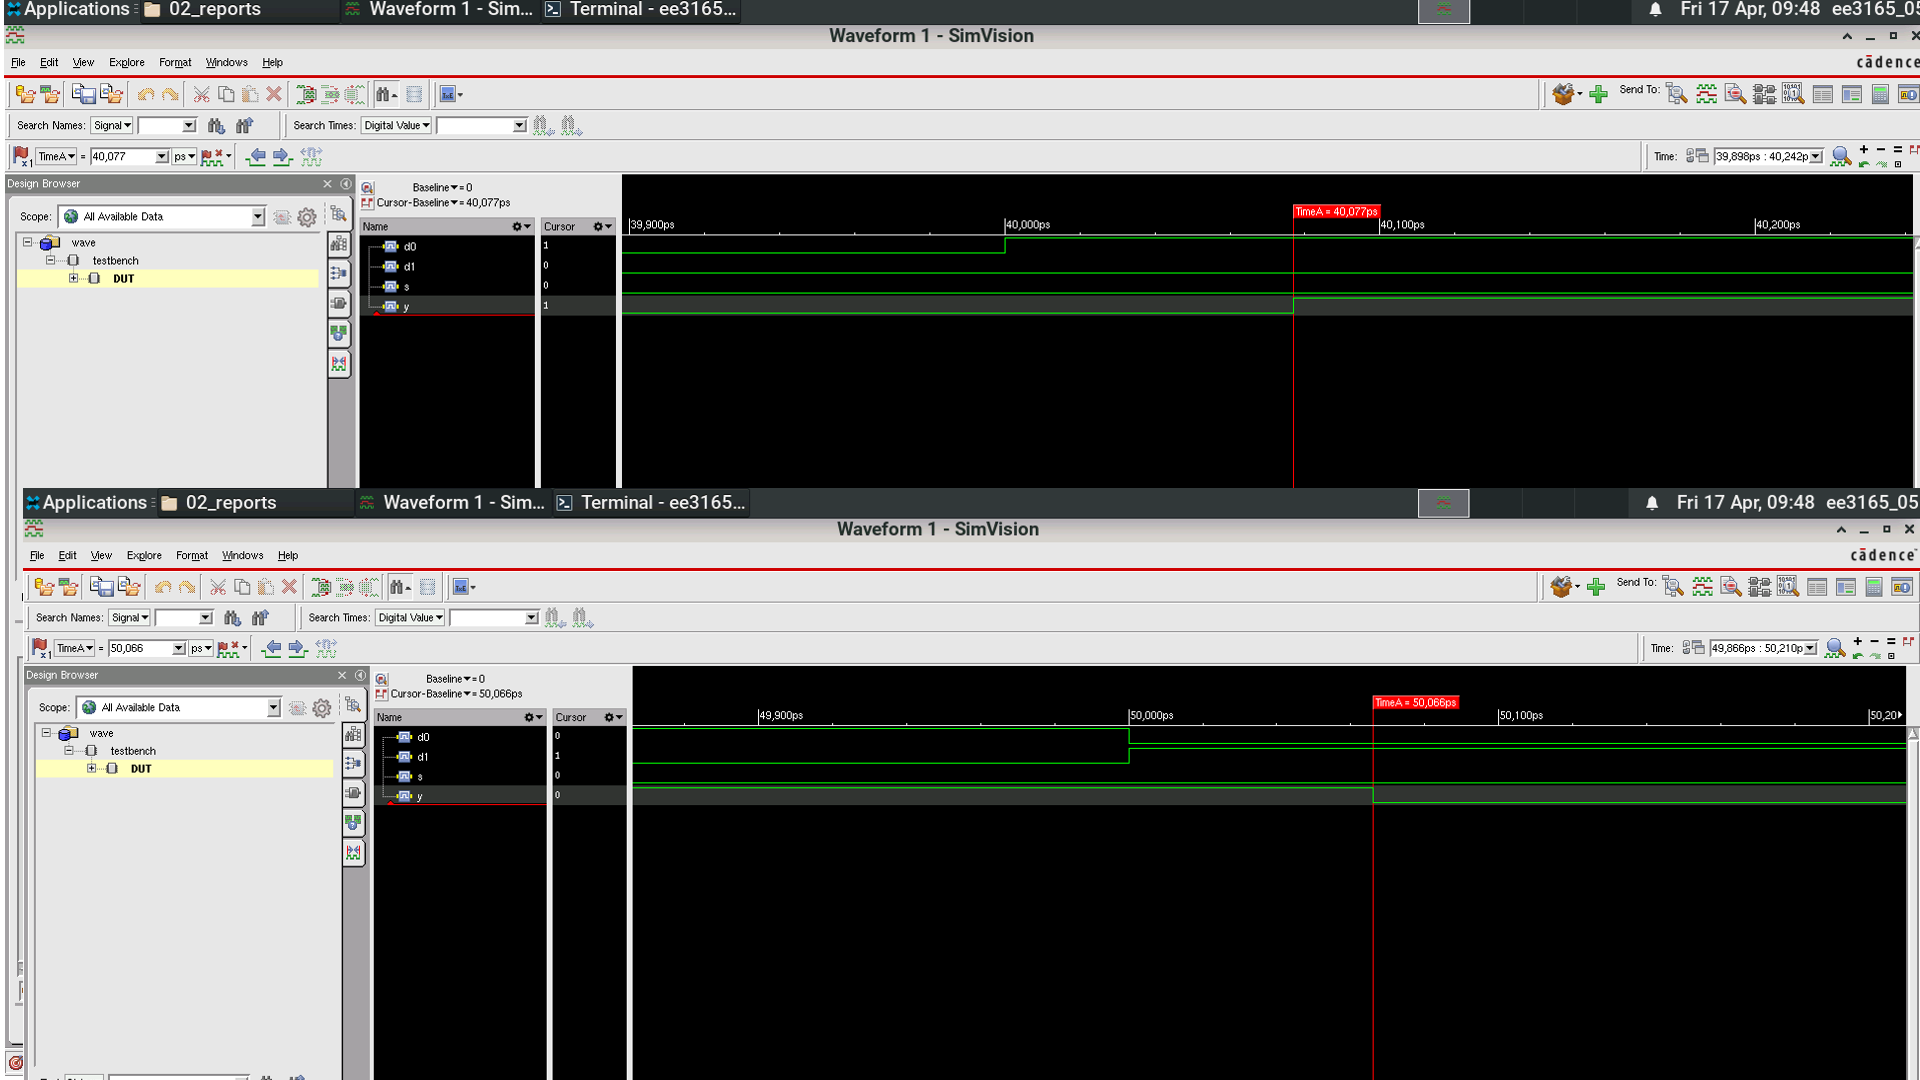
\includegraphics[width=\textwidth]{figures/exp1_mux_lvt_slow_1v0.png}
        \caption{Góc LVT Slow (slow\_vdd1v0)}
        \label{fig:mux_lvt_slow_1v0}
    \end{subfigure}
    \caption{Dạng sóng đo độ trễ cổng MUX sử dụng LVT tại 1.0V. Hình ảnh đại diện cho đường dẫn D0$\rightarrow$Y.}
    \label{fig:mux_lvt_comparison_1v0}
\end{figure}

\textbf{Nhận xét đặc tính LVT tại 1.0V:}
\begin{itemize}
    \item \textbf{Giải quyết điểm nghẽn thời gian:} Việc sử dụng thư viện LVT tại 1.0V đã mang lại hiệu quả rõ rệt. So với góc chậm nhất của HVT ($0.203ns$), LVT đã kéo giảm độ trễ sườn lên của \texttt{D0} xuống chỉ còn $0.077ns$, và đường \texttt{S$\rightarrow$Y} xuống $0.080ns$. Khi hệ thống buộc phải hoạt động ở chế độ tiết kiệm điện, LVT là giải pháp sống còn để đảm bảo luồng dữ liệu không bị nghẽn tại các bộ dồn kênh.
    \item \textbf{Gia tăng công suất tĩnh:} Sự cải thiện về tốc độ phải đánh đổi bằng mức tiêu thụ $2.71 \times 10^{-8}W$ ở góc chậm nhất, do dòng rò không thể triệt tiêu hoàn toàn.
\end{itemize}

\textbf{Khảo sát đặc tính LVT tại điều kiện 1.2V (Điện áp danh định):}

\begin{figure}[H]
    \centering
    \begin{subfigure}[b]{0.48\textwidth}
        \centering
        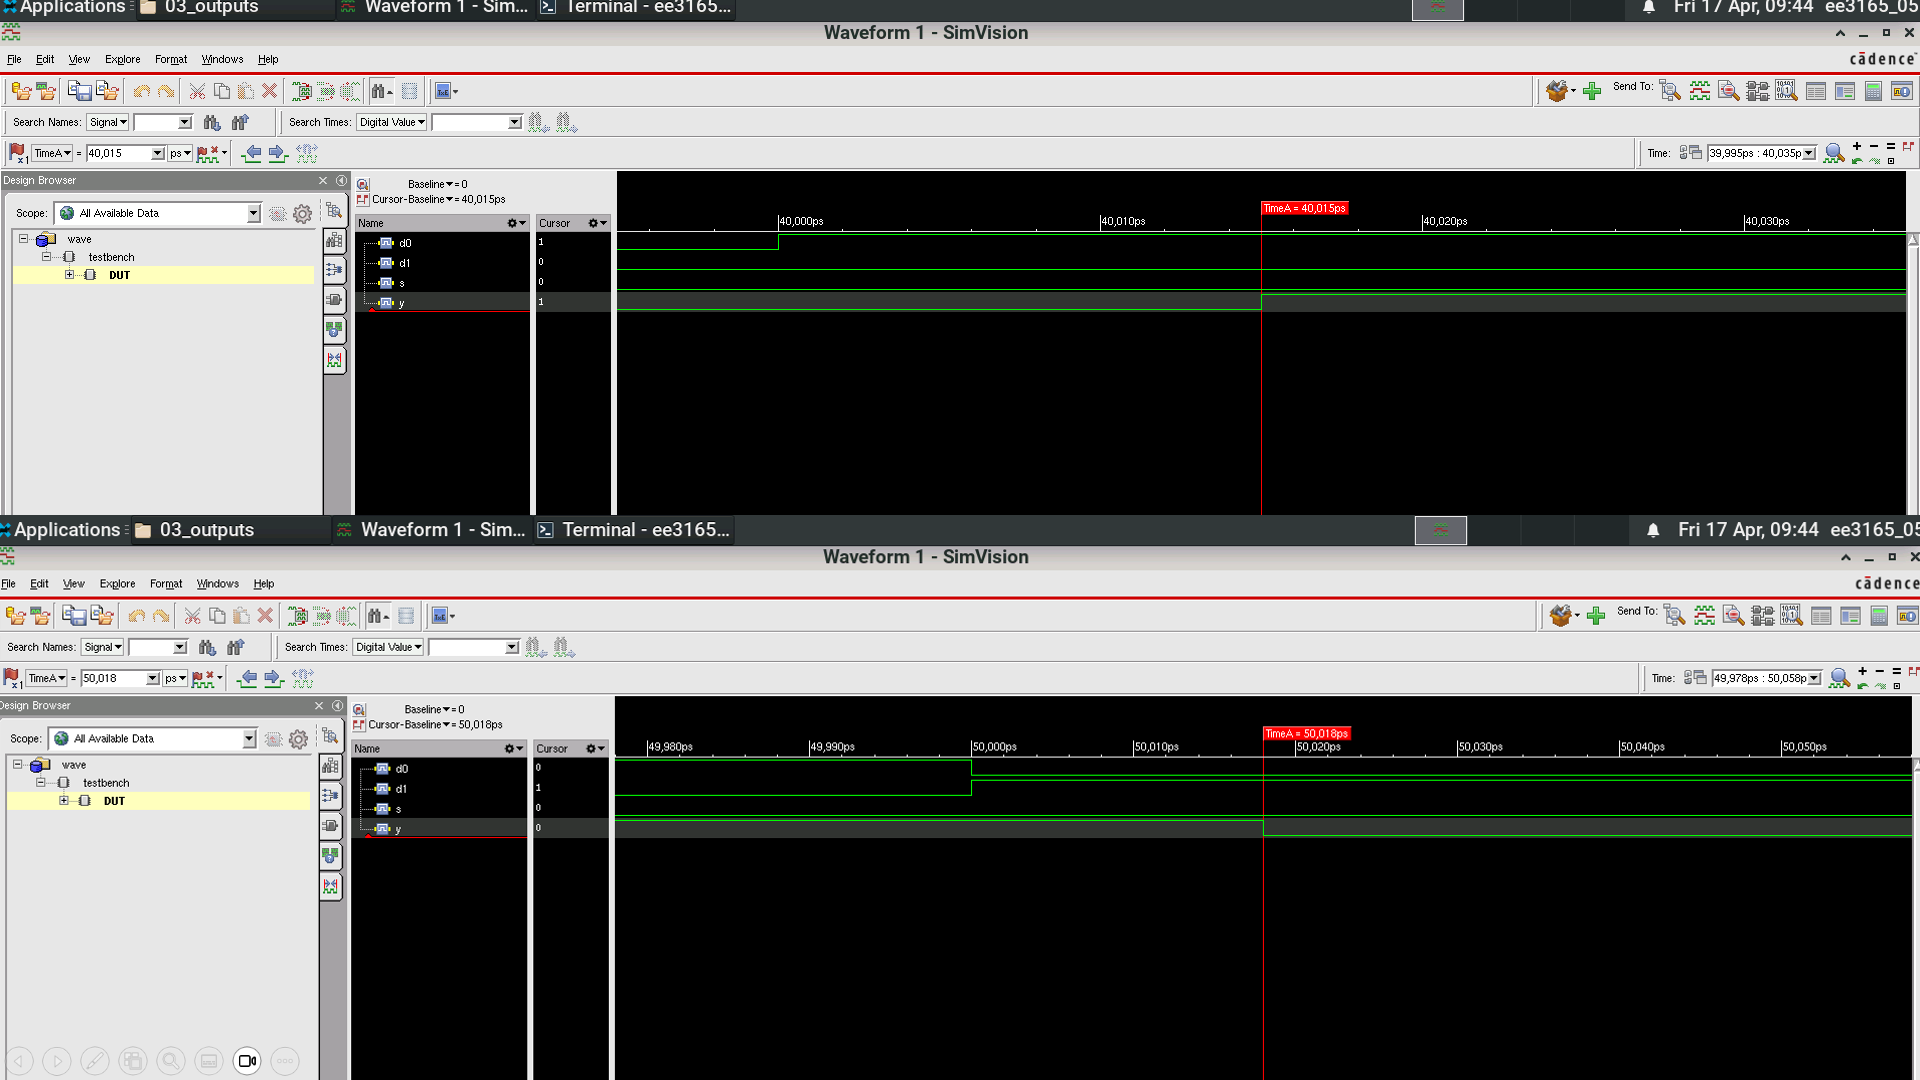
\includegraphics[width=\textwidth]{figures/exp1_mux_lvt_fast_1v2.png}
        \caption{Góc LVT Fast (fast\_vdd1v2)}
        \label{fig:mux_lvt_fast_1v2}
    \end{subfigure}
    \hfill
    \begin{subfigure}[b]{0.48\textwidth}
        \centering
        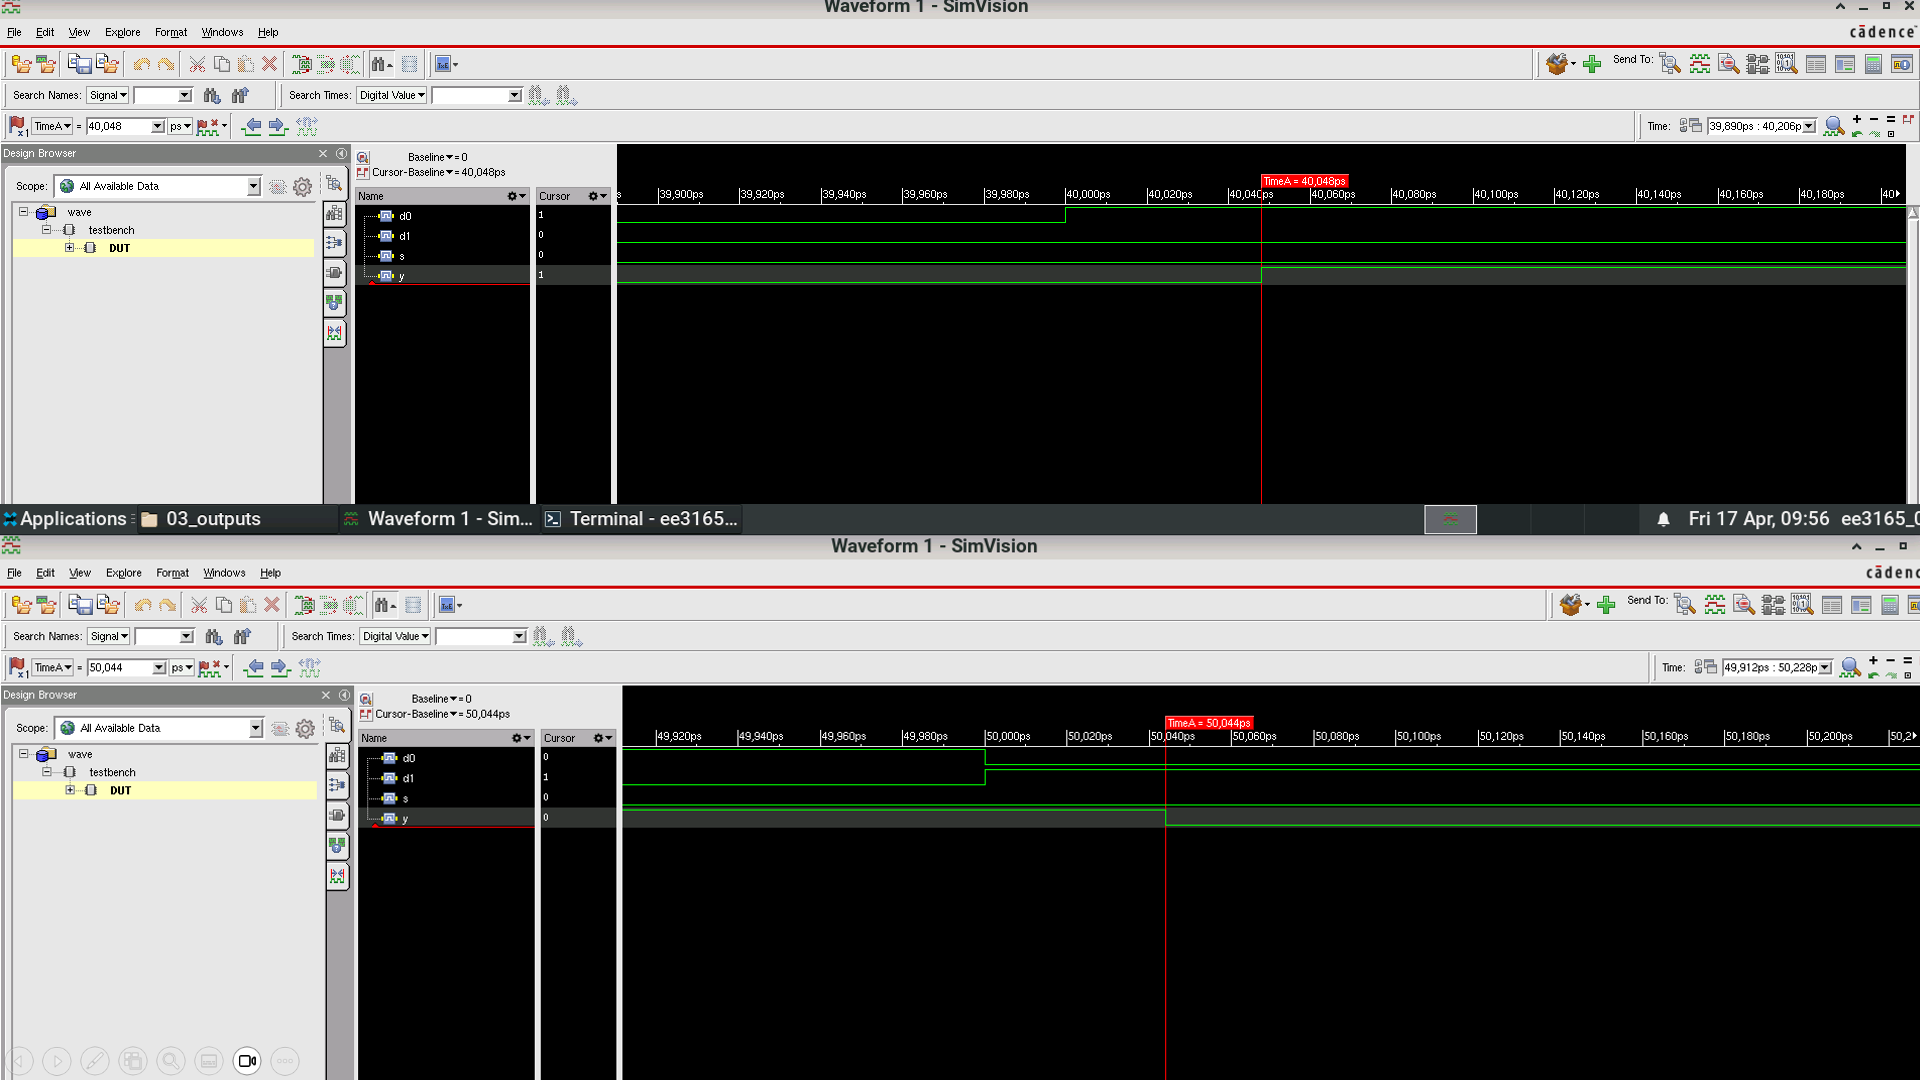
\includegraphics[width=\textwidth]{figures/exp1_mux_lvt_slow_1v2.png}
        \caption{Góc LVT Slow (slow\_vdd1v2)}
        \label{fig:mux_lvt_slow_1v2}
    \end{subfigure}
    \caption{Dạng sóng đo độ trễ cổng MUX sử dụng LVT tại 1.2V. Hình ảnh đại diện cho đường dẫn D0$\rightarrow$Y.}
    \label{fig:mux_lvt_comparison_1v2}
\end{figure}

\textbf{Nhận xét đặc tính LVT tại 1.2V:}
\begin{itemize}
    \item \textbf{Hiệu năng cực hạn:} Tại góc vận hành lý tưởng nhất, MUX loại bỏ hoàn toàn hiện tượng suy hao sườn xung. Mọi tín hiệu đều mất chưa tới $0.020ns$ để truyền qua mạch, đáp ứng các hệ thống đòi hỏi xung nhịp rất cao.
    \item \textbf{Đỉnh điểm tiêu thụ điện:} Đây là góc cấu hình "nóng" nhất của MUX với công suất tổng cộng lên tới $6.48 \times 10^{-8}W$. Thiết kế không nên lạm dụng thư viện này ngoại trừ các đường truyền dữ liệu bắt buộc phải tối ưu hóa thời gian thiết lập.
\end{itemize}

\paragraph{C. Kết luận} 
Phân tích bộ dồn kênh MUX làm rõ khái niệm độ trễ phụ thuộc đường dẫn trong thiết kế vi mạch. Do tín hiệu chọn (\texttt{S}) luôn phải đi qua nhiều tầng vật lý hơn, nó thường quyết định độ trễ tổng thể của linh kiện. Với diện tích cố định $2.394 \mu m^2$, kỹ sư thiết kế tối ưu hóa sẽ ưu tiên sử dụng thư viện LVT chỉ cho đường tín hiệu \texttt{S} để tăng tốc độ lựa chọn, trong khi giữ các nhánh dữ liệu \texttt{D0/D1} ở dạng HVT để kìm hãm công suất rò rỉ.

\newpage
\subsubsection{FULL ADDER}
\begin{lstlisting}[style={prettyverilog}, caption={\texttt{code thiết kế Full Adder}}]
`timescale 1ns/1ps
module fa(
    input logic A, B, Ci,
      output logic S, Co);
    assign S = A^B^Ci;
    assign Co= A&B | Ci&A | Ci&B;
endmodule
\end{lstlisting}
\begin{lstlisting}[style={prettyverilog}, caption={\texttt{code testbench Full Adder}}]
`timescale 1ns/1ps
module tb_fa;
    logic A, B, Ci;
    logic S, Co;
    fa(.A(A), .B(B), .Ci(Ci), .S(S), .Co(Co));
    initial begin
        $dumpfile("fa_wave.vcd");
        $dumpvars(0, tb_fa);
        A = 0; B = 1; Ci = 0; #10;
        A = 0; B = 1; Ci = 1; #10;
        A = 0; B = 1; Ci = 0; #10;
        A = 0; B = 1; Ci = 0; #10;
        A = 1; B = 1; Ci = 0; #10;
        A = 0; B = 1; Ci = 0; #10;
        A = 1; B = 0; Ci = 0; #10;
        A = 1; B = 1; Ci = 0; #10;
        A = 1; B = 0; Ci = 0; #10;
        $finish;
    end
endmodule
\end{lstlisting}

Trước hết, Hình \ref{fig:exp1_fa} trình bày ký hiệu logic cơ bản của bộ cộng toàn phần Full Adder. Khối này thực hiện phép cộng 3 bit ngõ vào (\texttt{A}, \texttt{B}, \texttt{Cin}) và tạo ra 2 tín hiệu ngõ ra là tổng \texttt{Sum} và số nhớ \texttt{Cout}. 

\begin{figure}[H]
    \centering
    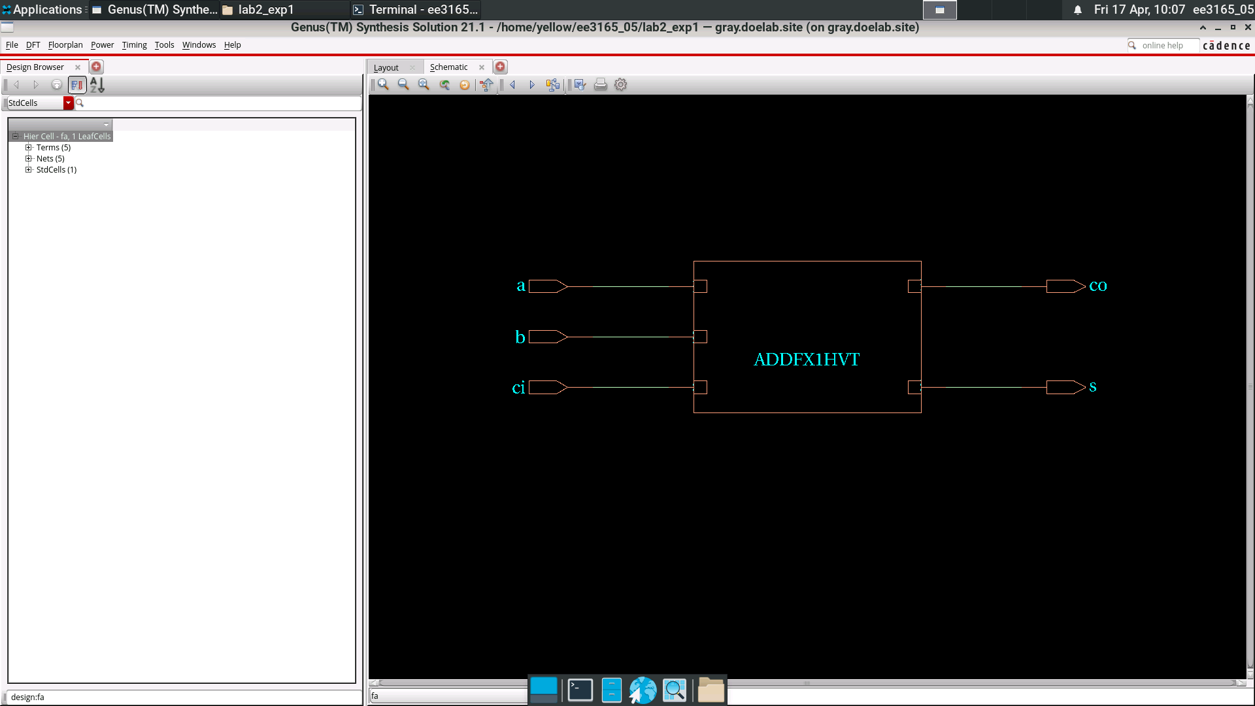
\includegraphics[width=0.6\textwidth]{figures/exp1_fa.png}
    \caption{Ký hiệu schematic và đặc tính logic cơ bản của khối Full Adder.}
    \label{fig:exp1_fa}
\end{figure}

Sau khi viết mã RTL, thiết kế được đưa vào công cụ Genus để thực hiện quá trình tổng hợp. Hình \ref{fig:exp1_fa_mapped} minh họa sơ đồ mức cổng của Full Adder sau khi được ánh xạ vào thư viện công nghệ 45nm. 

\begin{figure}[H]
    \centering
    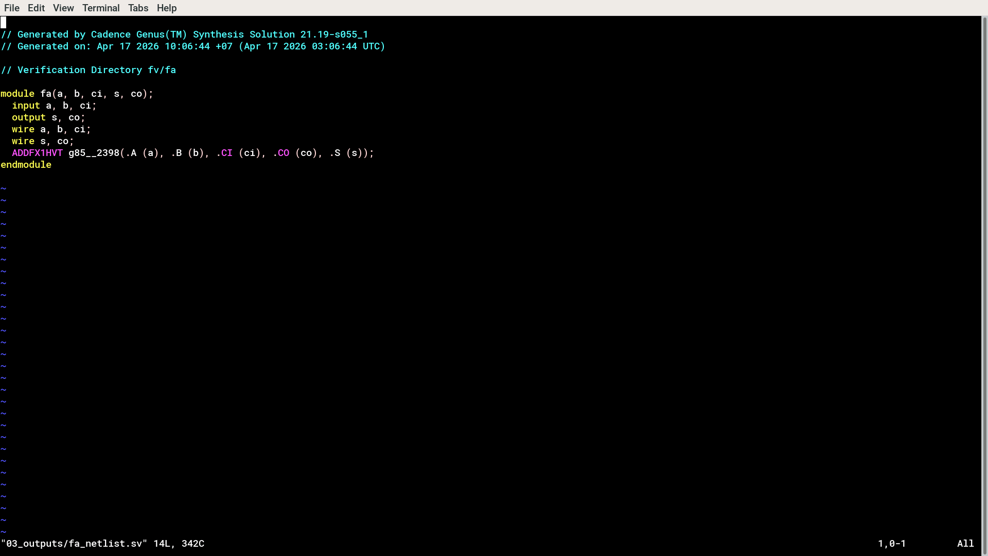
\includegraphics[width=0.7\textwidth]{figures/exp1_fa_mapped.png}
    \caption{Sơ đồ mức cổng của thiết kế Full Adder trên giao diện Genus.}
    \label{fig:exp1_fa_mapped}
\end{figure}

Do kiến trúc bên trong của Full Adder bao gồm nhiều cổng logic đa tầng, thời gian trễ truyền dẫn không đồng nhất trên các đường tín hiệu. Nhóm tiến hành đo đạc chi tiết 6 đường trễ cơ bản: \texttt{Cin$\rightarrow$Cout}, \texttt{A$\rightarrow$Cout}, \texttt{B$\rightarrow$Cout}, \texttt{Cin$\rightarrow$Sum}, \texttt{A$\rightarrow$Sum}, và \texttt{B$\rightarrow$Sum}. Để tối ưu việc trình bày, các đường trễ có chung ngõ vào sẽ được gộp chung vào một waveform và phân biệt bằng màu marker (Đỏ cho ngõ ra Cout, Xanh cho ngõ ra Sum).

% ====================================================================
% KHỐI A: THƯ VIỆN HVT
% ====================================================================
\paragraph{A. Thư viện High Threshold Voltage (HVT)}

Đặc tính của các cell HVT là dòng rò thấp nhưng độ trễ lớn hơn. Kết quả mô phỏng 8 góc quy trình cho 6 đường dẫn được tổng hợp trong bảng dưới đây:

\begin{table}[H]
\centering
\renewcommand{\arraystretch}{1.3}
\resizebox{\textwidth}{!}{
\begin{tabular}{|l|c|c|c|c|c|c|c|c|c|c|c|c|c|c|}
\hline
\multirow{2}{*}{\textbf{Library Name}} 
& \multirow{2}{*}{\textbf{Area}} 
& \multirow{2}{*}{\textbf{Power}} 
& \multicolumn{2}{c|}{\textbf{Cin$\rightarrow$Cout}}
& \multicolumn{2}{c|}{\textbf{A$\rightarrow$Cout}} 
& \multicolumn{2}{c|}{\textbf{B$\rightarrow$Cout}} 
& \multicolumn{2}{c|}{\textbf{Cin$\rightarrow$Sum}} 
& \multicolumn{2}{c|}{\textbf{A$\rightarrow$Sum}} 
& \multicolumn{2}{c|}{\textbf{B$\rightarrow$Sum}} \\
\cline{4-15}
& & 
& \textbf{Rise} & \textbf{Fall}
& \textbf{Rise} & \textbf{Fall}
& \textbf{Rise} & \textbf{Fall}
& \textbf{Rise} & \textbf{Fall}
& \textbf{Rise} & \textbf{Fall}
& \textbf{Rise} & \textbf{Fall} \\
\hline
fast\_vdd1v0\_basicCells\_hvt 
& 5.130 & 8.72063e-08 & 0.044 & 0.051 & 0.048 & 0.053 & 0.048 & 0.054 & 0.075 & 0.077 & 0.080 & 0.081 & 0.083 & 0.080 \\ \hline
fast\_vdd1v2\_basicCells\_hvt 
& 5.130 & 1.35372e-07 & 0.031 & 0.036 & 0.034 & 0.039 & 0.034 & 0.038 & 0.054 & 0.054 & 0.058 & 0.057 & 0.059 & 0.056 \\ \hline
slow\_vdd1v0\_basicCells\_hvt 
& 5.130 & 5.36985e-08 & 0.267 & 0.173 & 0.288 & 0.174 & 0.282 & 0.176 & 0.383 & 0.362 & 0.418 & 0.400 & 0.403 & 0.389 \\ \hline
slow\_vdd1v2\_basicCells\_hvt 
& 5.130 & 8.40672e-08 & 0.112 & 0.086 & 0.124 & 0.089 & 0.121 & 0.089 & 0.160 & 0.163 & 0.175 & 0.181 & 0.176 & 0.176 \\ \hline
\end{tabular}
}
\caption{Tổng hợp thông số Area, Power và Delay 6 đường dẫn của Full Adder (HVT).}
\label{tab:exp1_fa_hvt_params}
\end{table}

\textbf{1. Khảo sát HVT tại điện áp thấp (VDD = 1.0V)}

\begin{figure}[H] \centering
    \begin{subfigure}[b]{0.48\textwidth} \centering 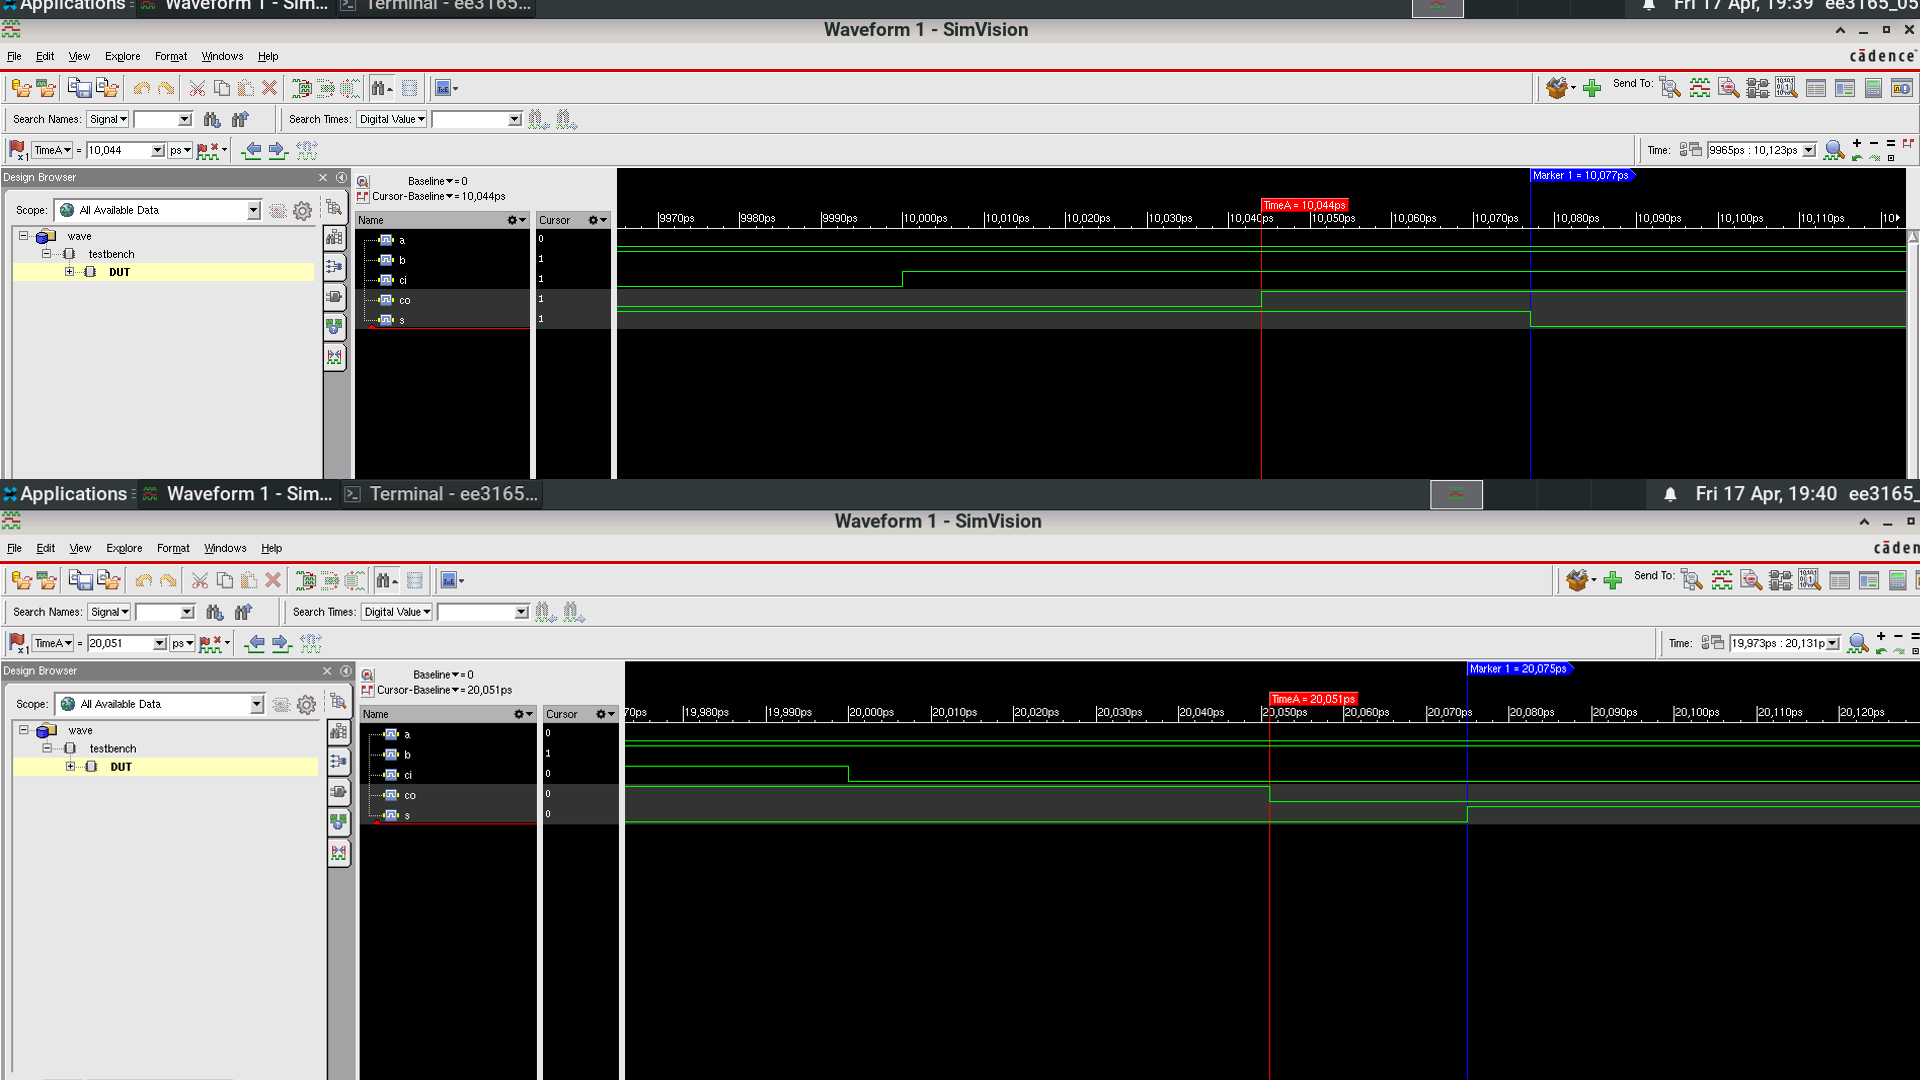
\includegraphics[width=\textwidth]{figures/fa_hvt_1v0_cin_fast.png} \caption{Góc Fast} \end{subfigure} \hfill
    \begin{subfigure}[b]{0.48\textwidth} \centering 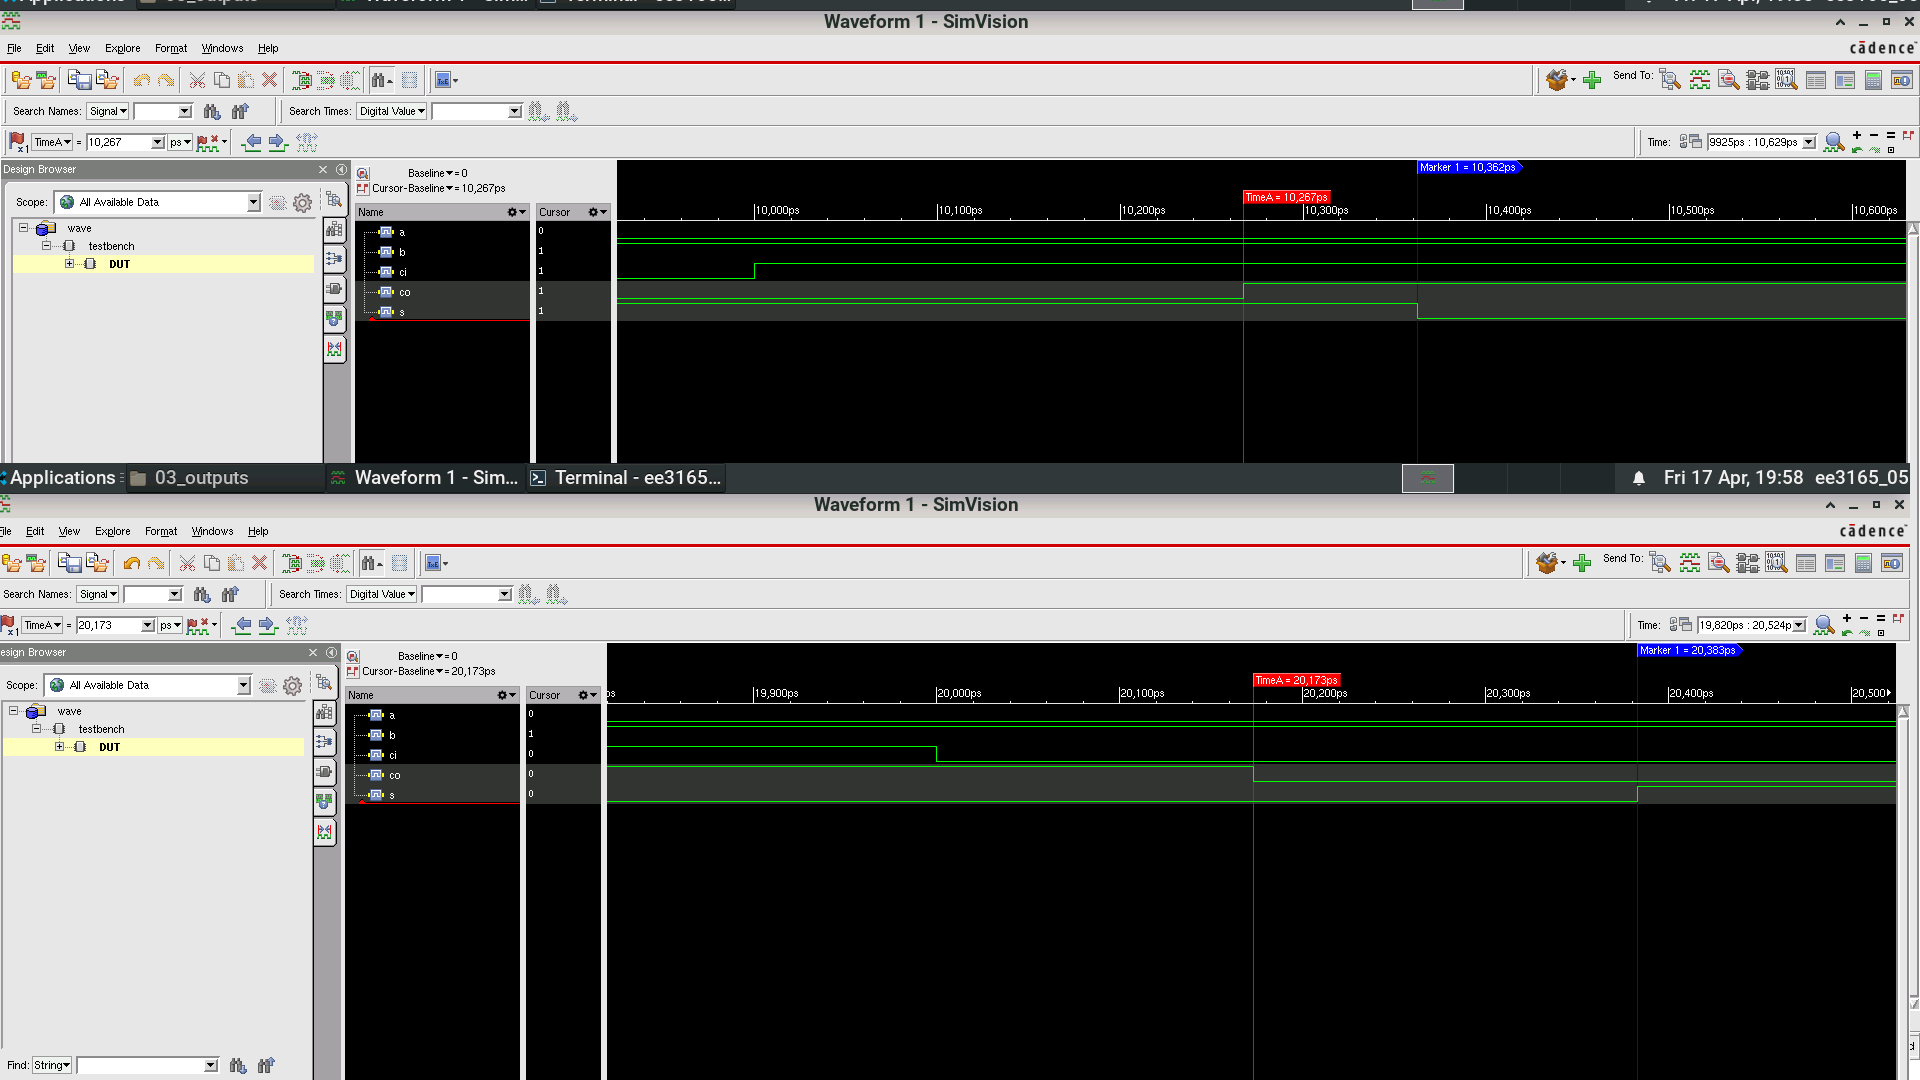
\includegraphics[width=\textwidth]{figures/fa_hvt_1v0_cin_slow.png} \caption{Góc Slow} \end{subfigure}
    \caption{Dạng sóng đo độ trễ từ \textbf{Cin} tới các ngõ ra tại HVT 1.0V. Marker màu đỏ đo \texttt{Cin$\rightarrow$Cout}, màu xanh đo \texttt{Cin$\rightarrow$Sum}.}
\end{figure}

\begin{figure}[H] \centering
    \begin{subfigure}[b]{0.48\textwidth} \centering 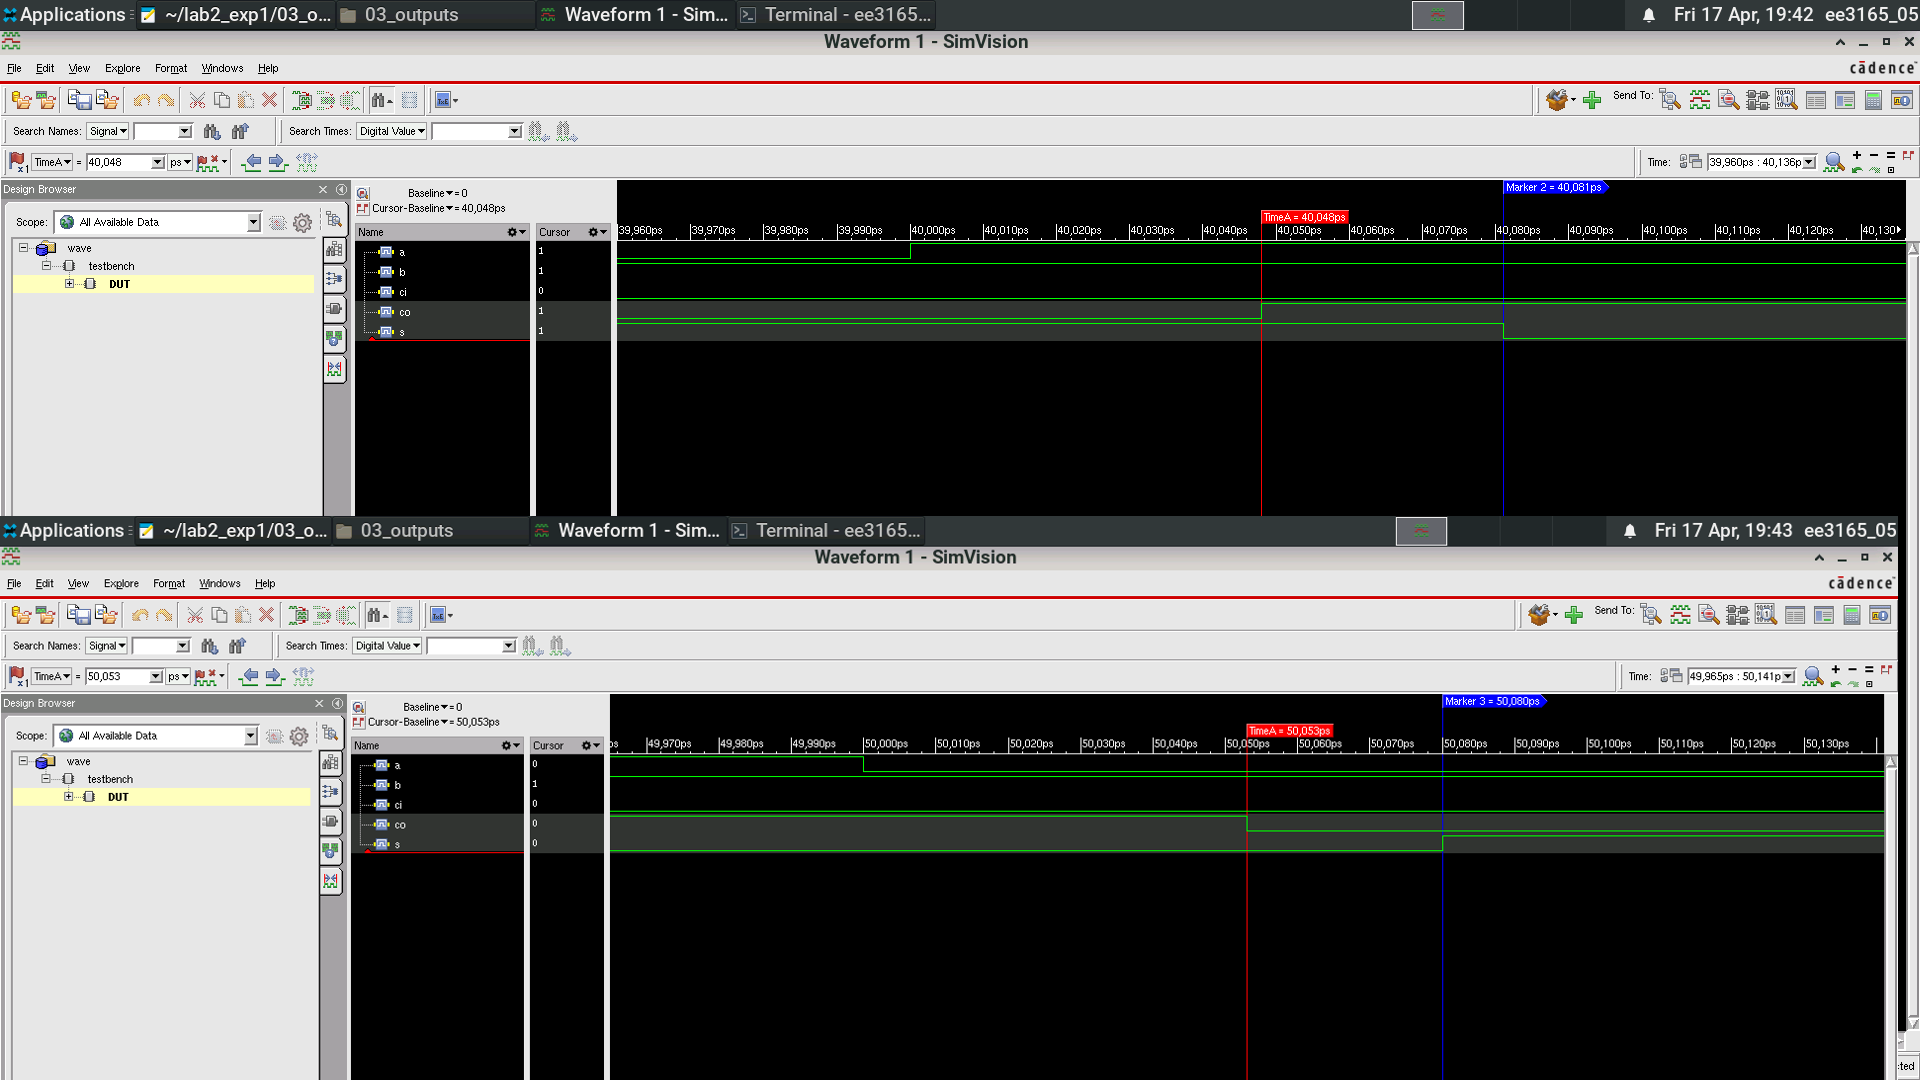
\includegraphics[width=\textwidth]{figures/fa_hvt_1v0_a_fast.png} \caption{Góc Fast} \end{subfigure} \hfill
    \begin{subfigure}[b]{0.48\textwidth} \centering 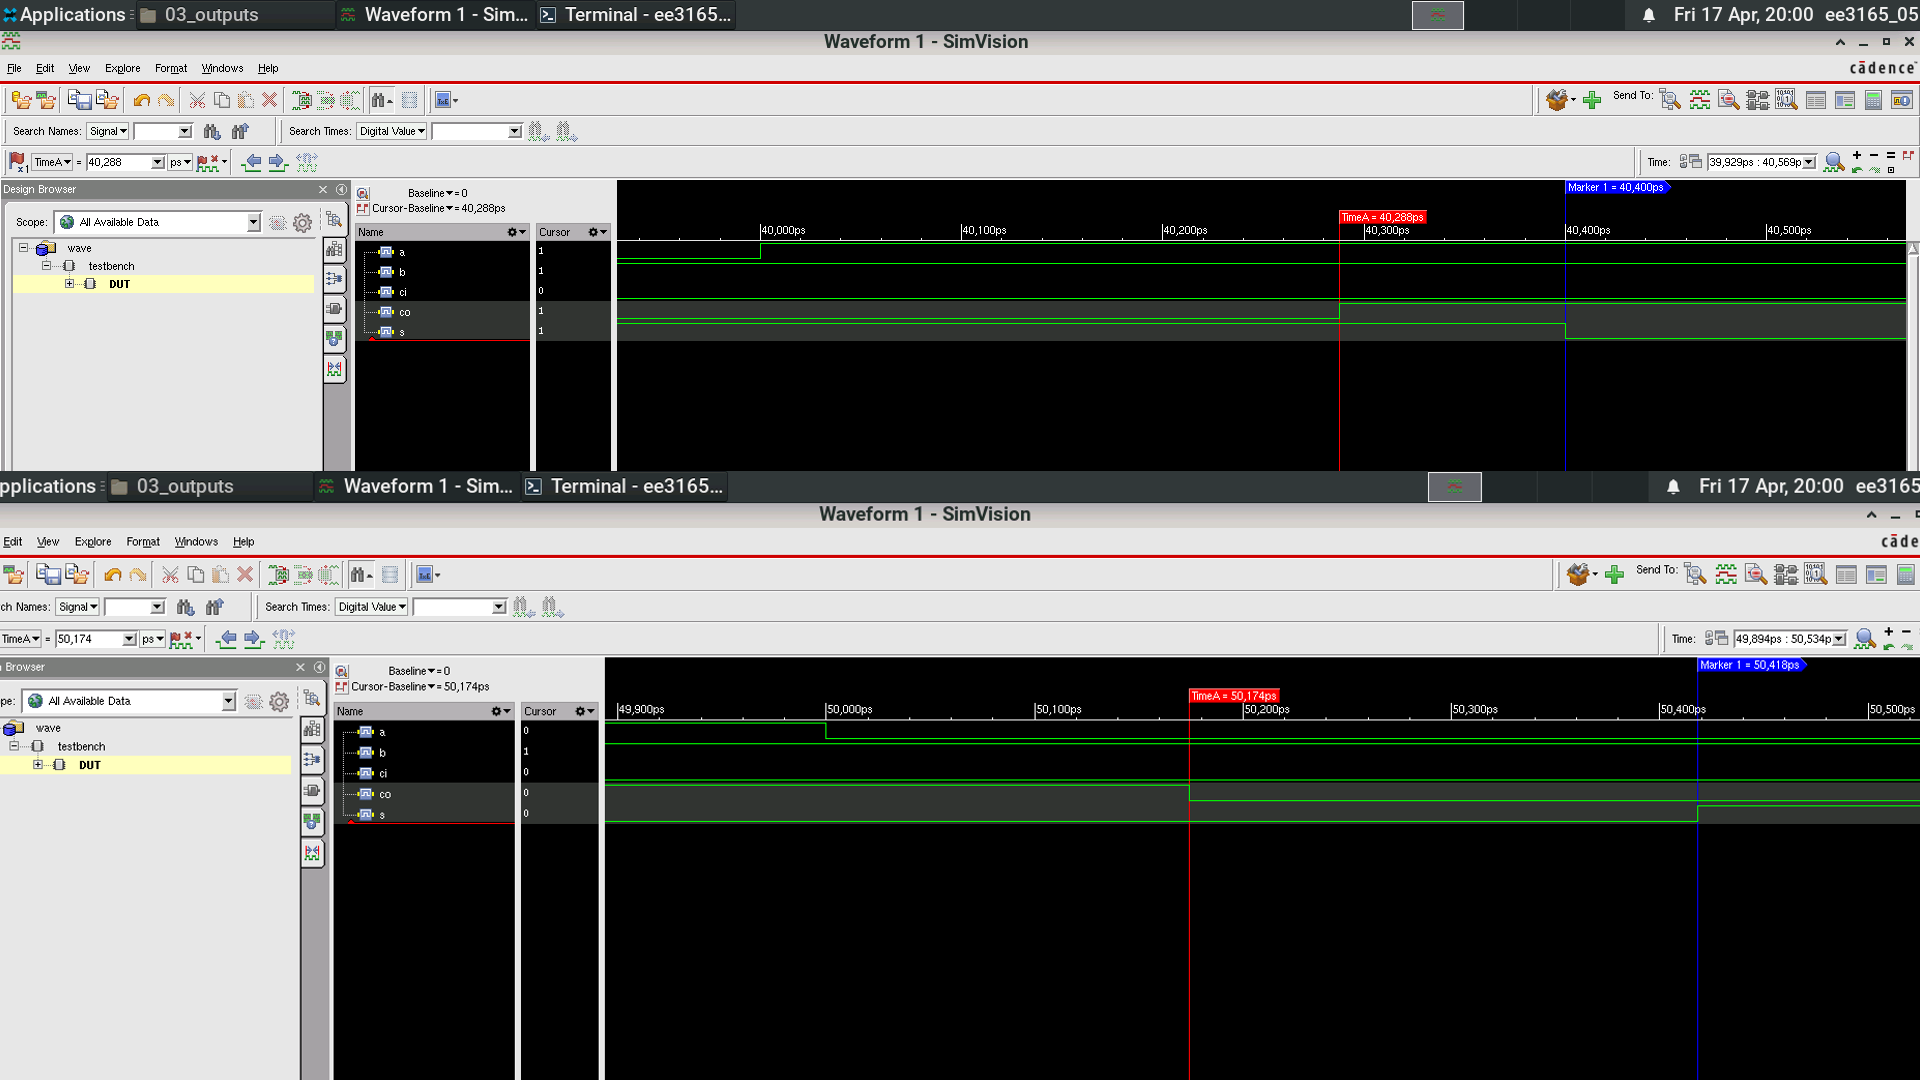
\includegraphics[width=\textwidth]{figures/fa_hvt_1v0_a_slow.png} \caption{Góc Slow} \end{subfigure}
    \caption{Dạng sóng đo độ trễ từ \textbf{A} tới các ngõ ra tại HVT 1.0V. Marker màu đỏ đo \texttt{A$\rightarrow$Cout}, màu xanh đo \texttt{A$\rightarrow$Sum}.}
\end{figure}

\begin{figure}[H] \centering
    \begin{subfigure}[b]{0.48\textwidth} \centering 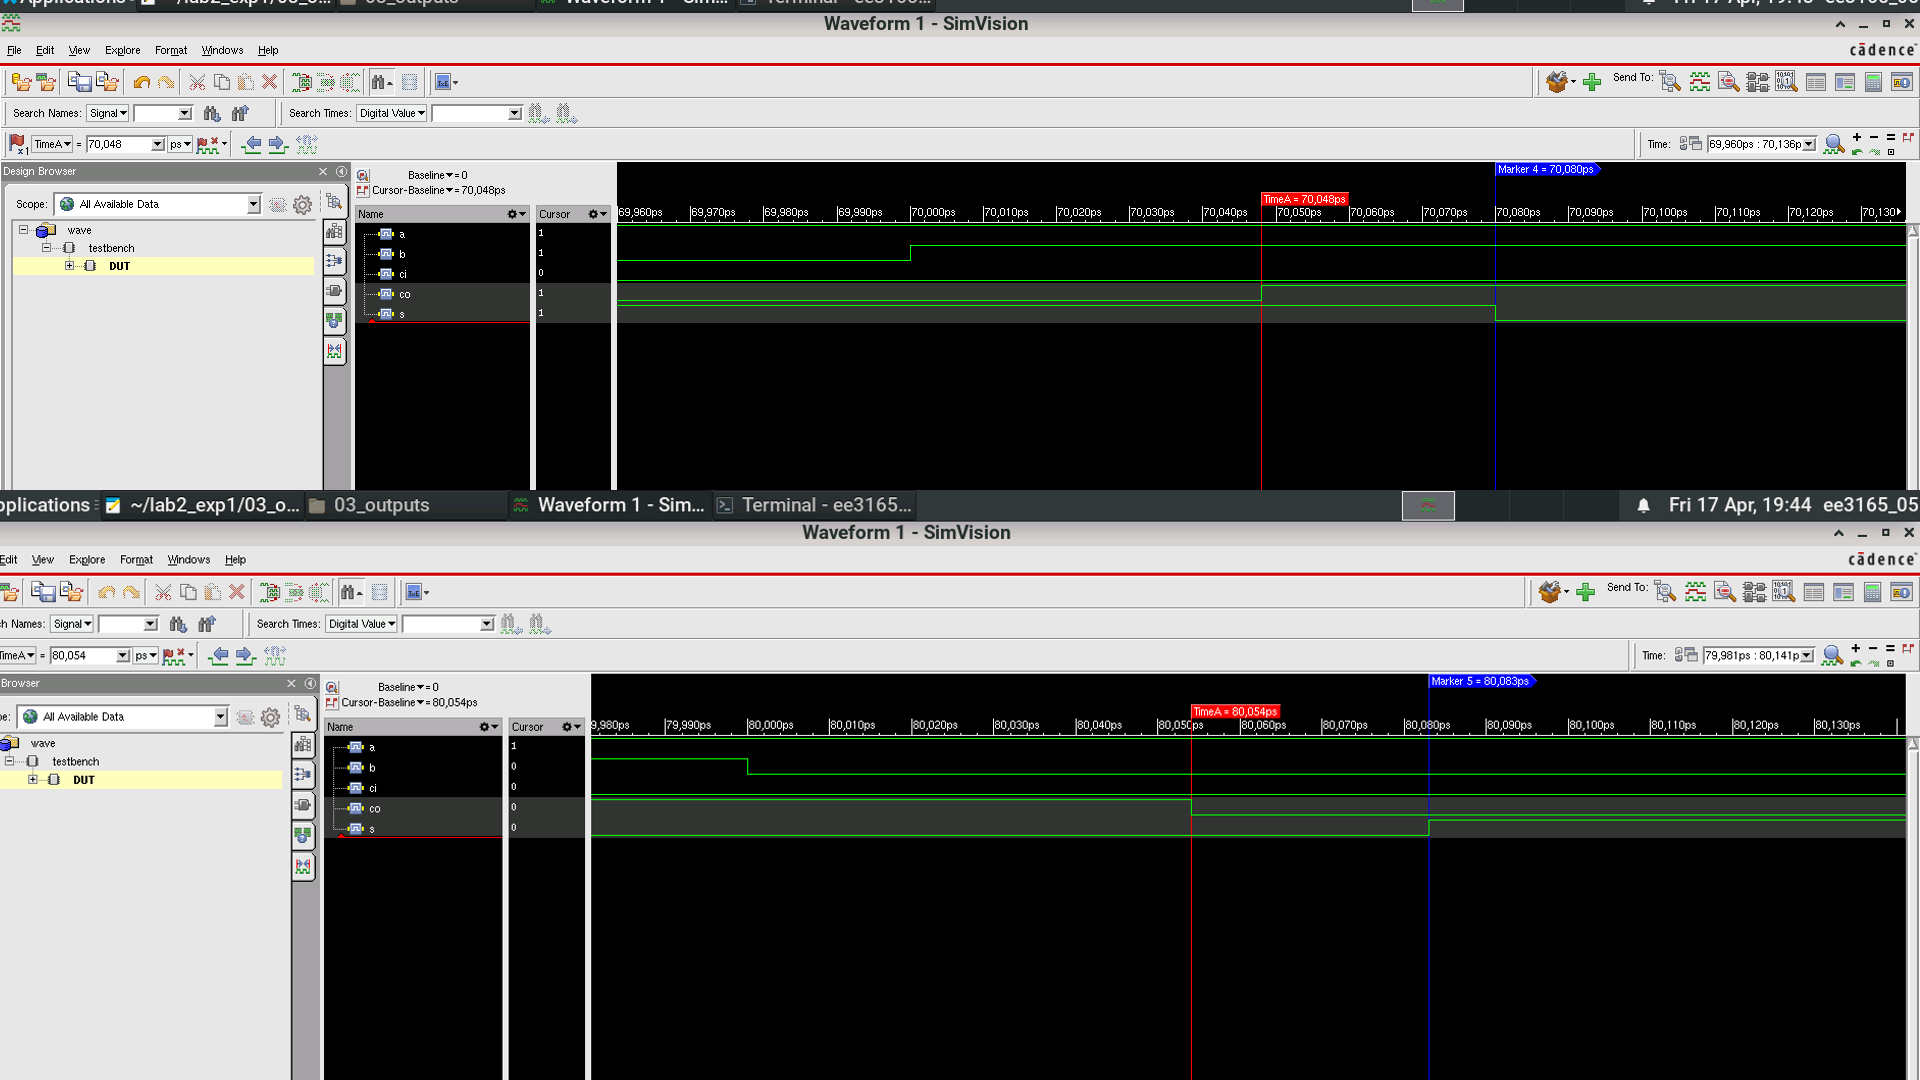
\includegraphics[width=\textwidth]{figures/fa_hvt_1v0_b_fast.png} \caption{Góc Fast} \end{subfigure} \hfill
    \begin{subfigure}[b]{0.48\textwidth} \centering 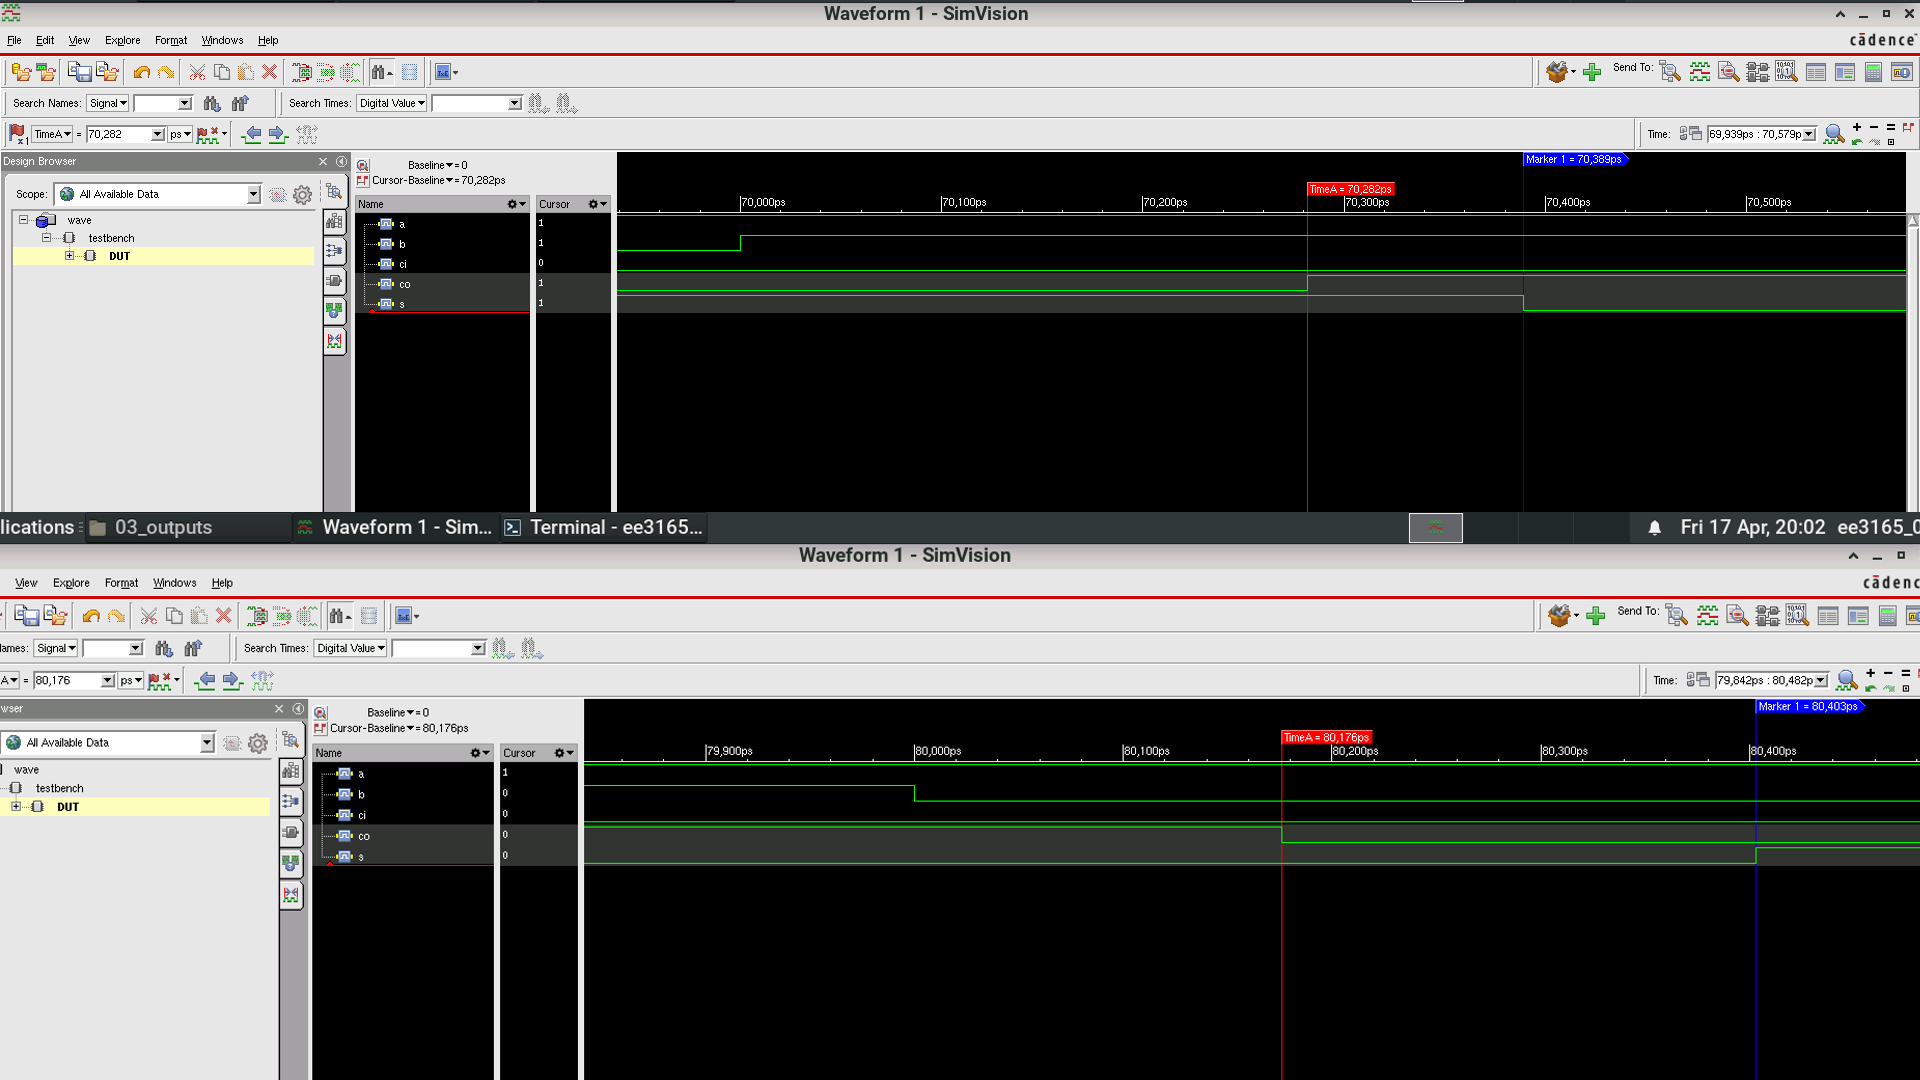
\includegraphics[width=\textwidth]{figures/fa_hvt_1v0_b_slow.png} \caption{Góc Slow} \end{subfigure}
    \caption{Dạng sóng đo độ trễ từ \textbf{B} tới các ngõ ra tại HVT 1.0V. Marker màu đỏ đo \texttt{B$\rightarrow$Cout}, màu xanh đo \texttt{B$\rightarrow$Sum}.}
\end{figure}

\textbf{Nhận xét (HVT - 1.0V):} Dựa trên số liệu đo đạc tại mức điện áp 1.0V, ta có thể phân tích chi tiết độ phức tạp của khối cộng toàn phần:
\begin{itemize}
    \item \textbf{Sự chênh lệch giữa mạch tổng và mạch nhớ:} Bảng số liệu chỉ ra rằng độ trễ đi ra ngõ Sum luôn lớn hơn ngõ Cout. Ví dụ tại góc chậm nhất, đường \texttt{A$\rightarrow$Sum} mất 0.418 ns để nạp tụ sườn lên, trong khi đường \texttt{A$\rightarrow$Cout} chỉ mất 0.288 ns. Điều này là do tín hiệu Sum phải đi qua các cổng XOR nhiều tầng, tạo ra độ sâu logic lớn hơn nhiều so với mạch tạo số nhớ Cout.
    \item \textbf{Hiện tượng suy hao tốc độ diện rộng:} Ở 1.0V, dòng điện bão hòa suy yếu khiến toàn bộ các đường dẫn đều bị chậm lại đáng kể. Đường truyền số nhớ \texttt{Cin$\rightarrow$Cout} chạm mức 0.267 ns ở sườn lên, tạo ra nguy cơ vi phạm thời gian thiết lập rất lớn nếu ghép nối thành bộ cộng nhiều bit.
    \item \textbf{Ưu thế năng lượng:} Nhờ sử dụng thư viện HVT ở điện áp thấp, công suất tiêu thụ tại góc chậm nhất được giữ ở mức cực kỳ an toàn, chỉ 5.36e-8 W.
\end{itemize}

\textbf{2. Khảo sát HVT tại điện áp danh định (VDD = 1.2V)}

\begin{figure}[H] \centering
    \begin{subfigure}[b]{0.48\textwidth} \centering 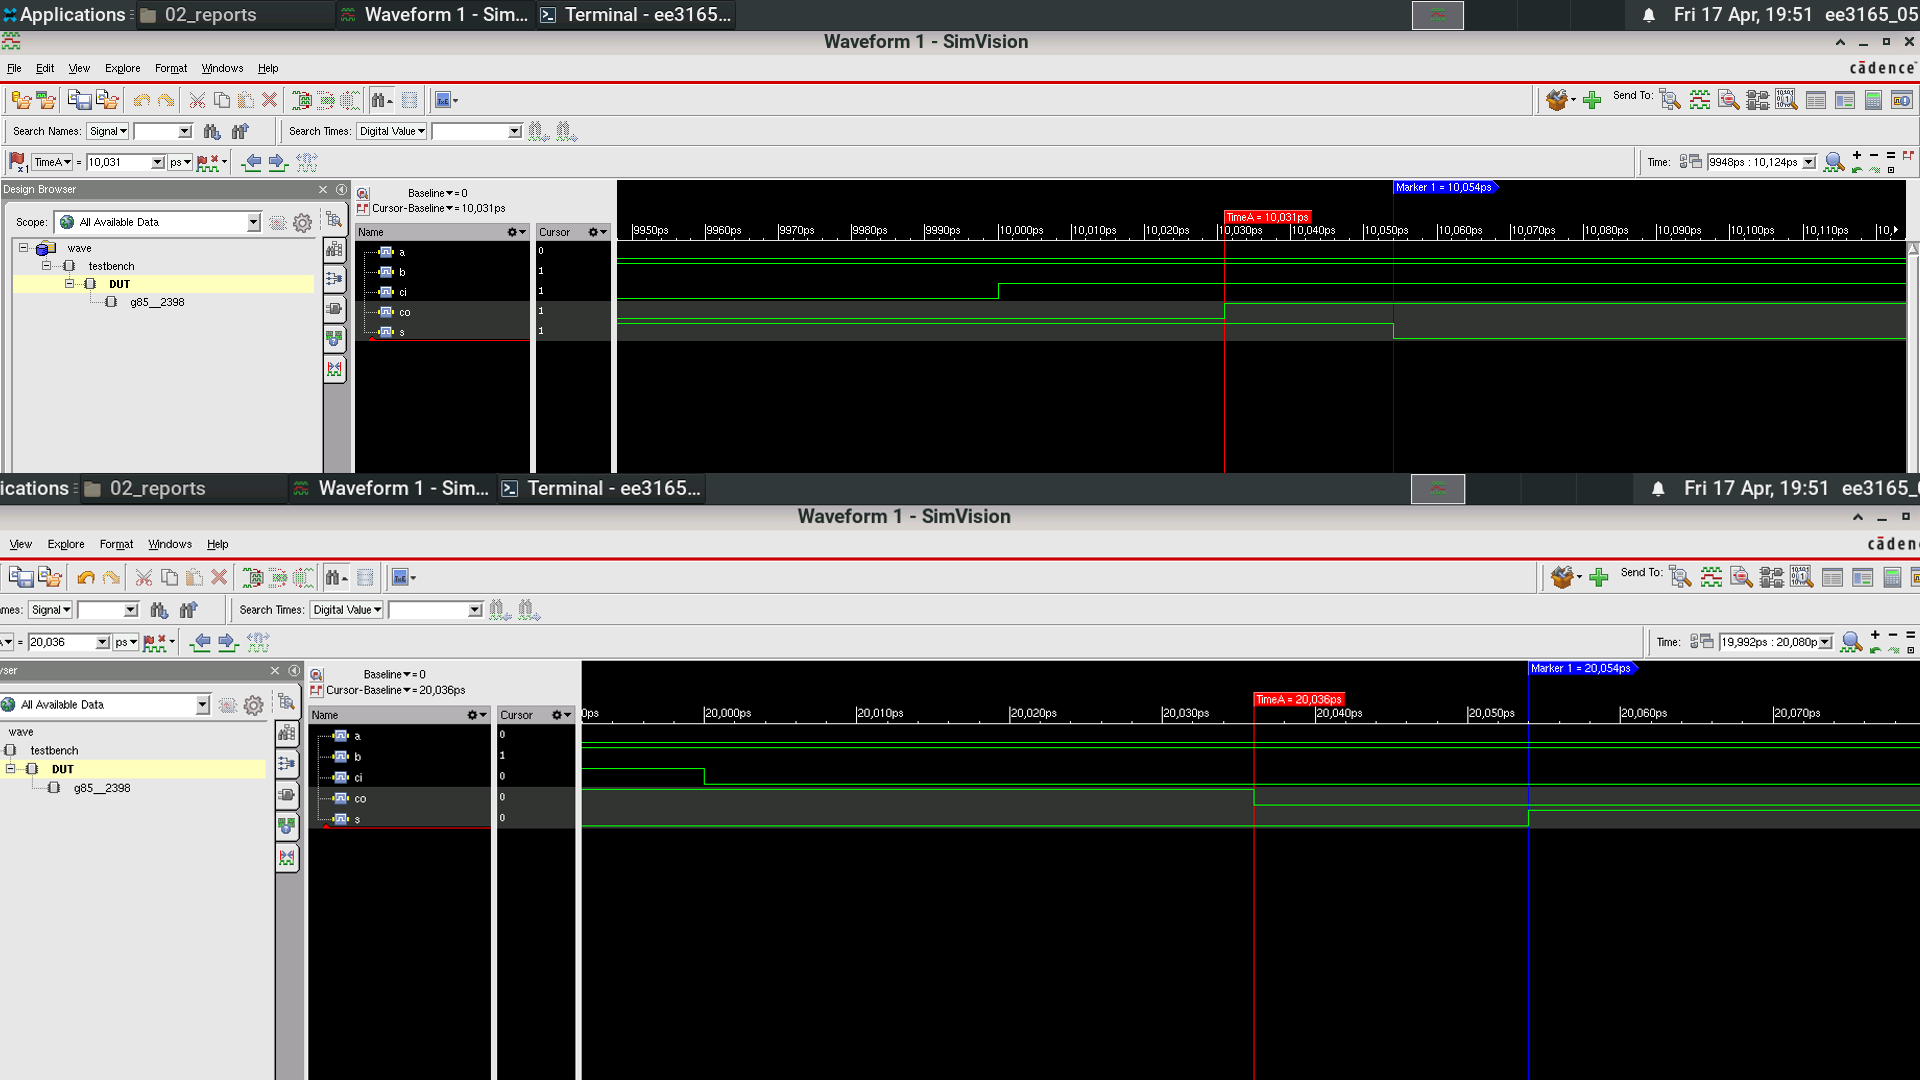
\includegraphics[width=\textwidth]{figures/fa_hvt_1v2_cin_fast.png} \caption{Góc Fast} \end{subfigure} \hfill
    \begin{subfigure}[b]{0.48\textwidth} \centering 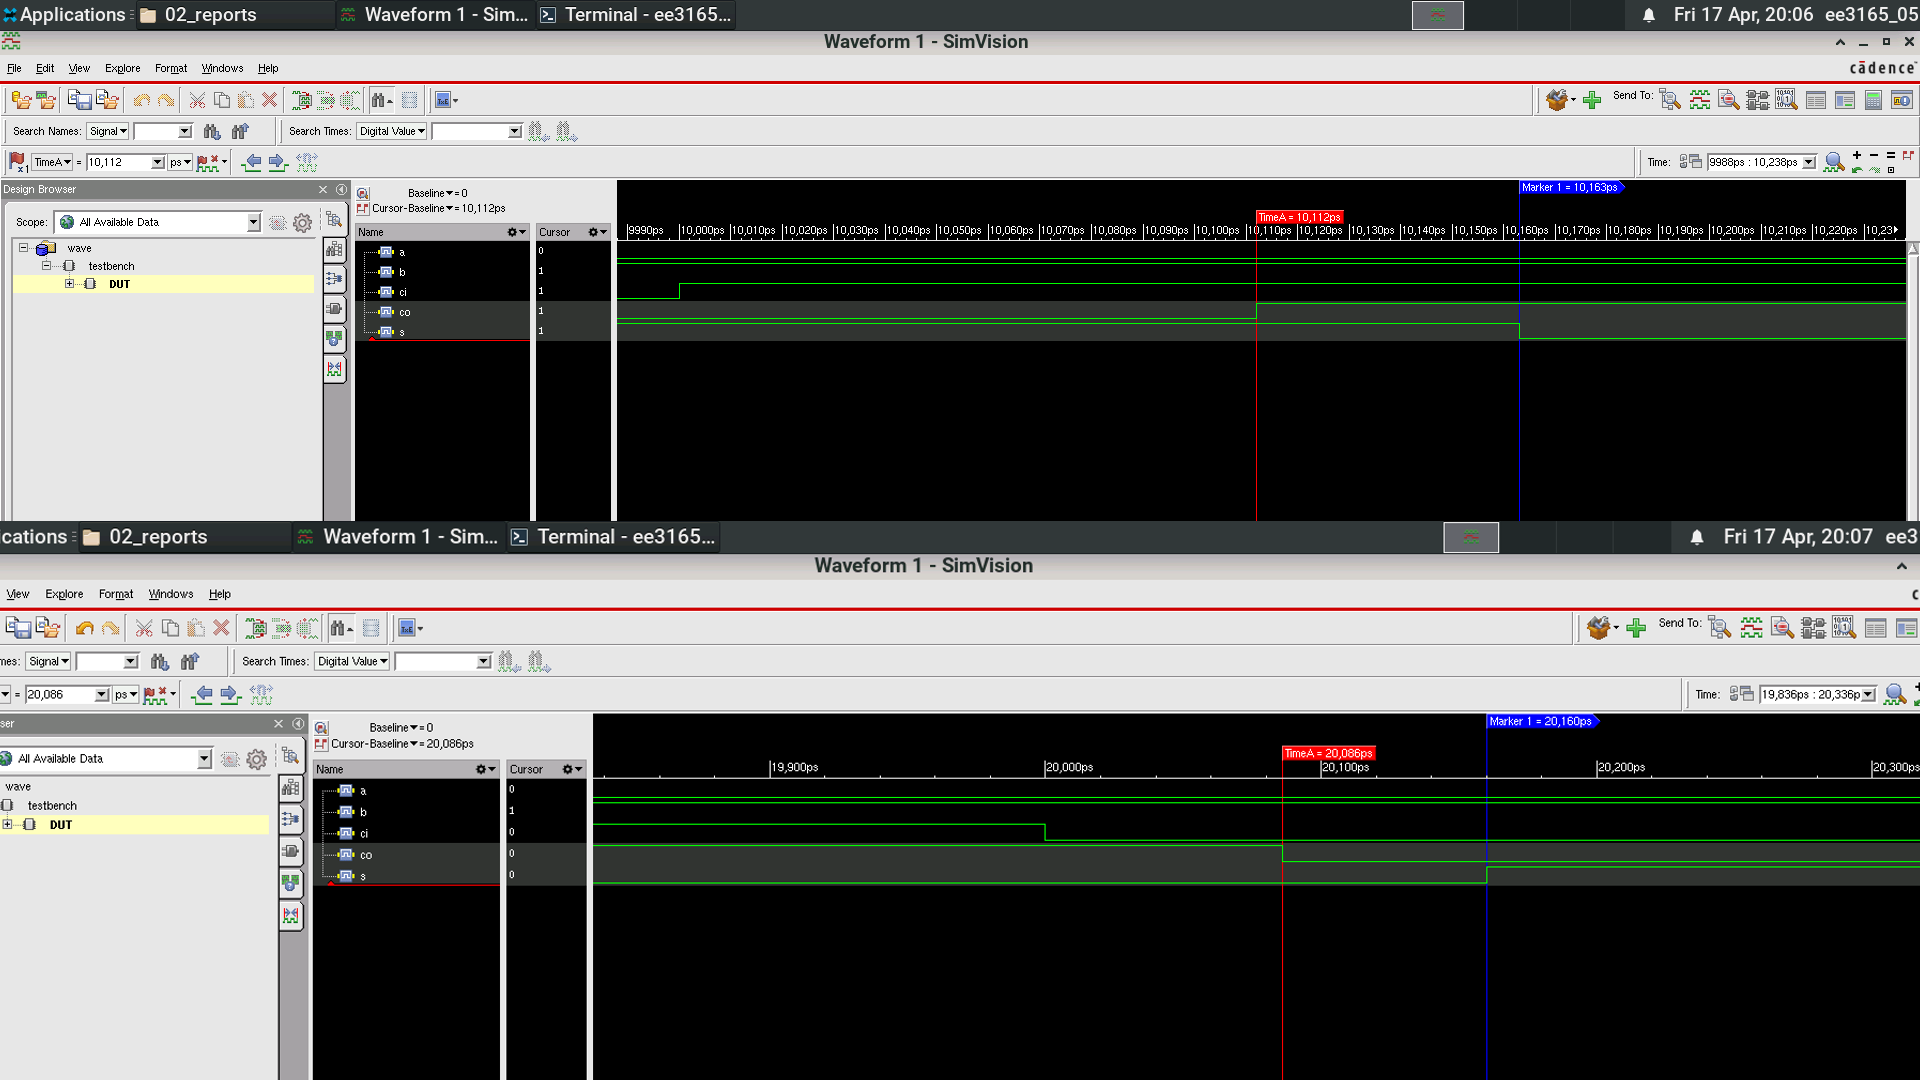
\includegraphics[width=\textwidth]{figures/fa_hvt_1v2_cin_slow.png} \caption{Góc Slow} \end{subfigure}
    \caption{Dạng sóng đo độ trễ từ \textbf{Cin} tới các ngõ ra tại HVT 1.2V (Marker Đỏ: Cout, Xanh: Sum).}
\end{figure}

\begin{figure}[H] \centering
    \begin{subfigure}[b]{0.48\textwidth} \centering 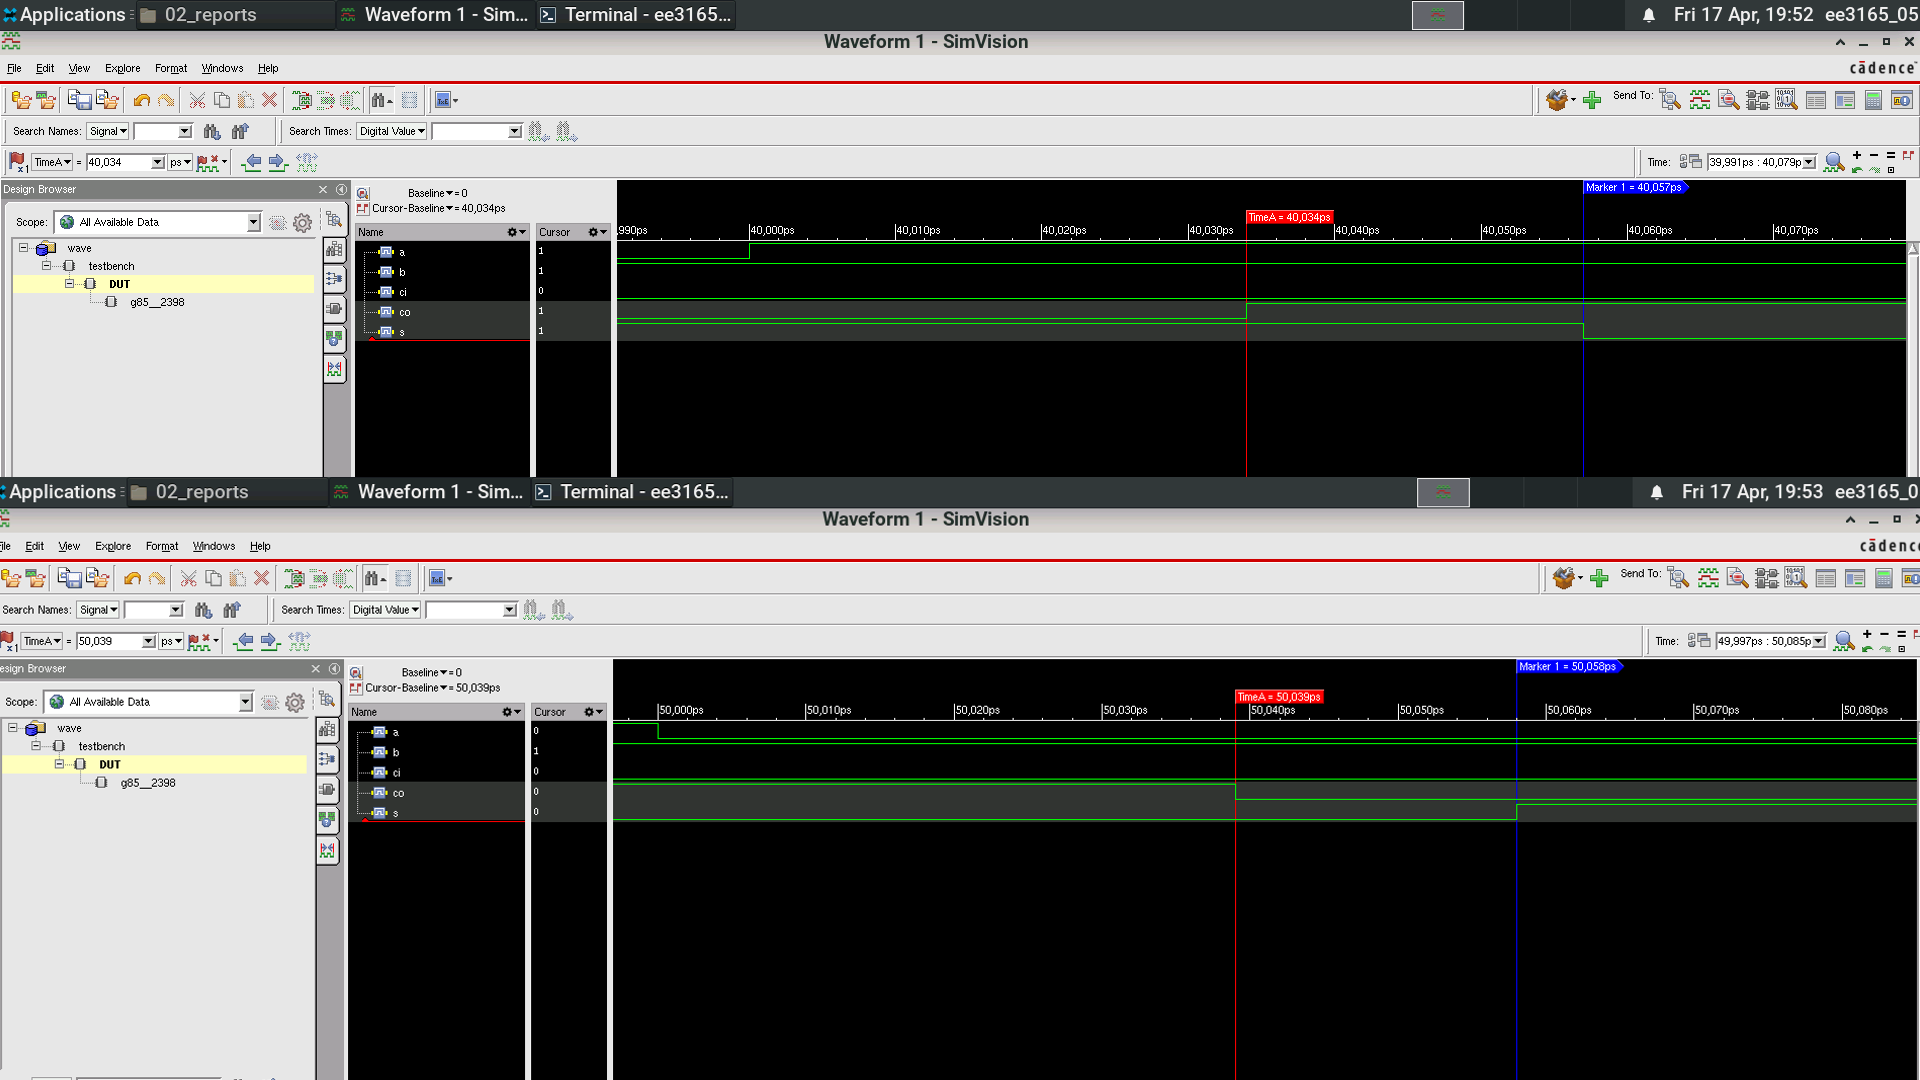
\includegraphics[width=\textwidth]{figures/fa_hvt_1v2_a_fast.png} \caption{Góc Fast} \end{subfigure} \hfill
    \begin{subfigure}[b]{0.48\textwidth} \centering 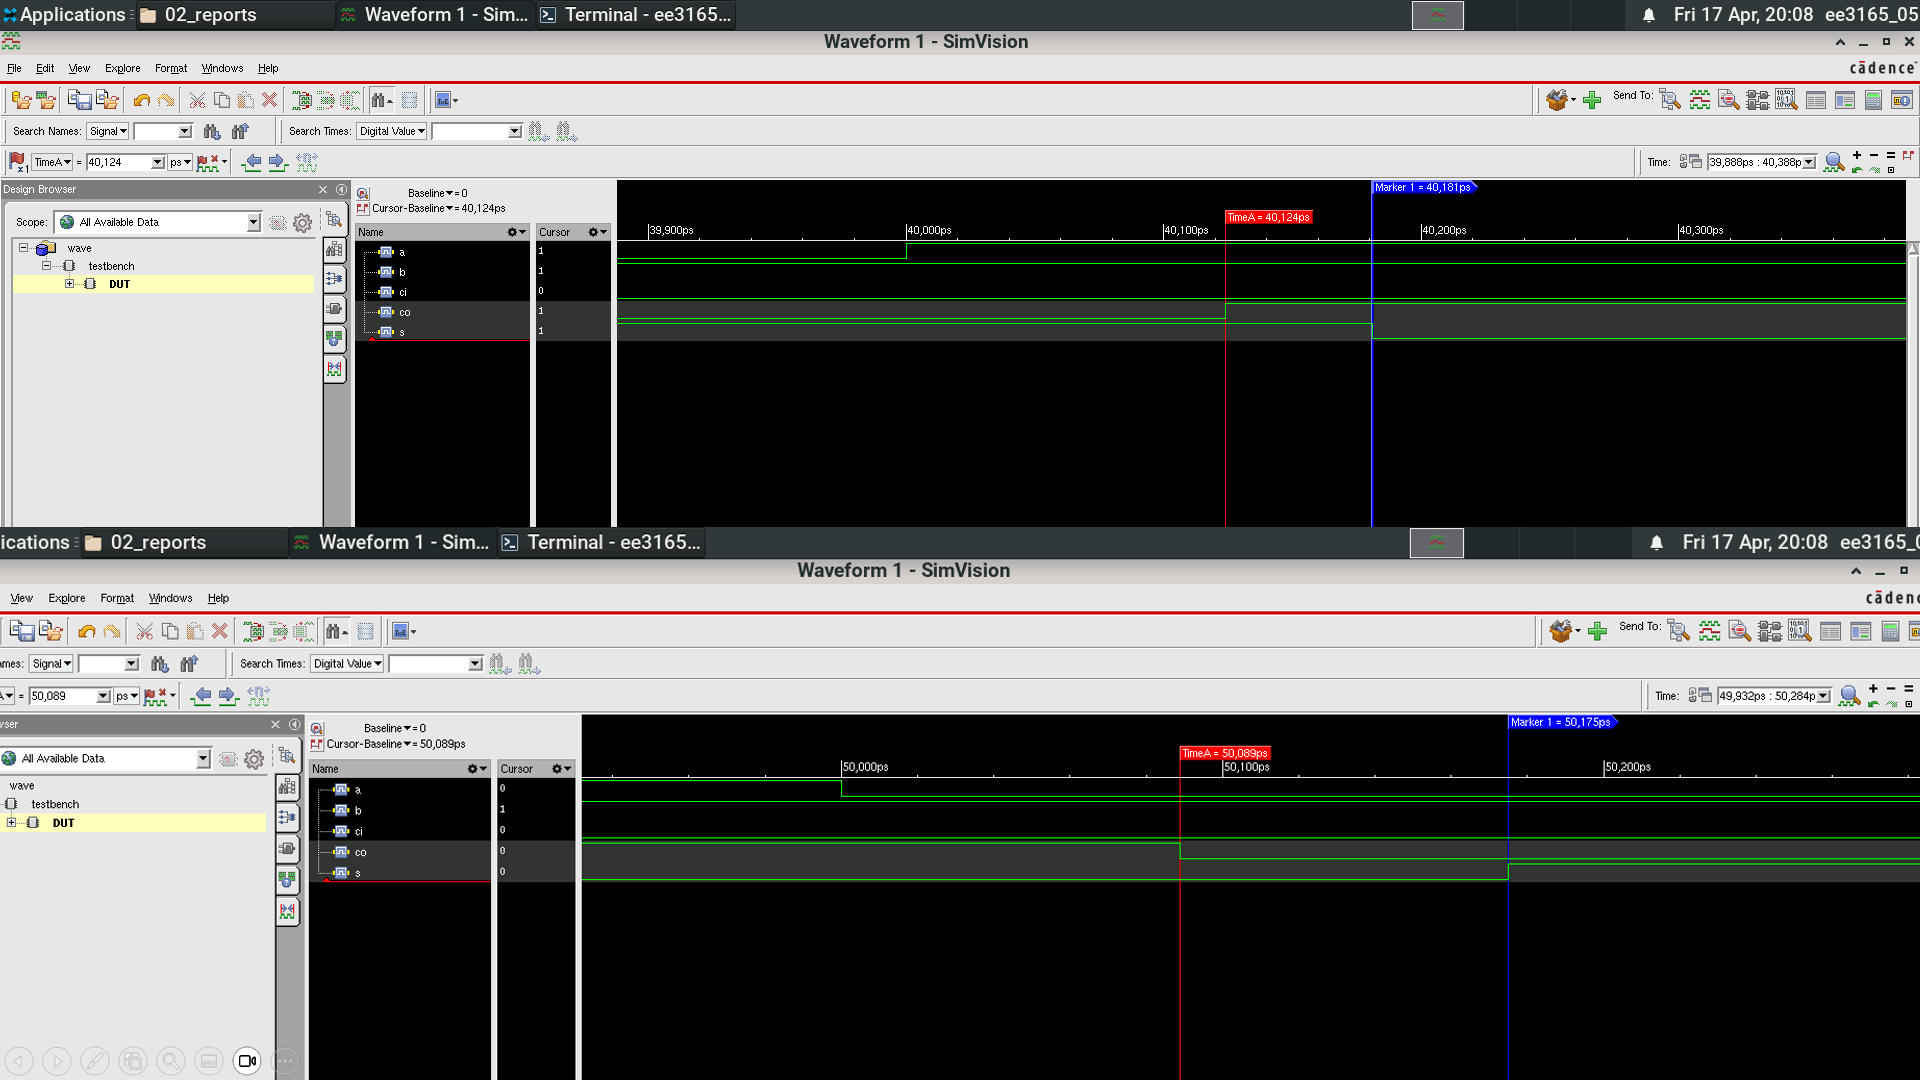
\includegraphics[width=\textwidth]{figures/fa_hvt_1v2_a_slow.png} \caption{Góc Slow} \end{subfigure}
    \caption{Dạng sóng đo độ trễ từ \textbf{A} tới các ngõ ra tại HVT 1.2V (Marker Đỏ: Cout, Xanh: Sum).}
\end{figure}

\begin{figure}[H] \centering
    \begin{subfigure}[b]{0.48\textwidth} \centering 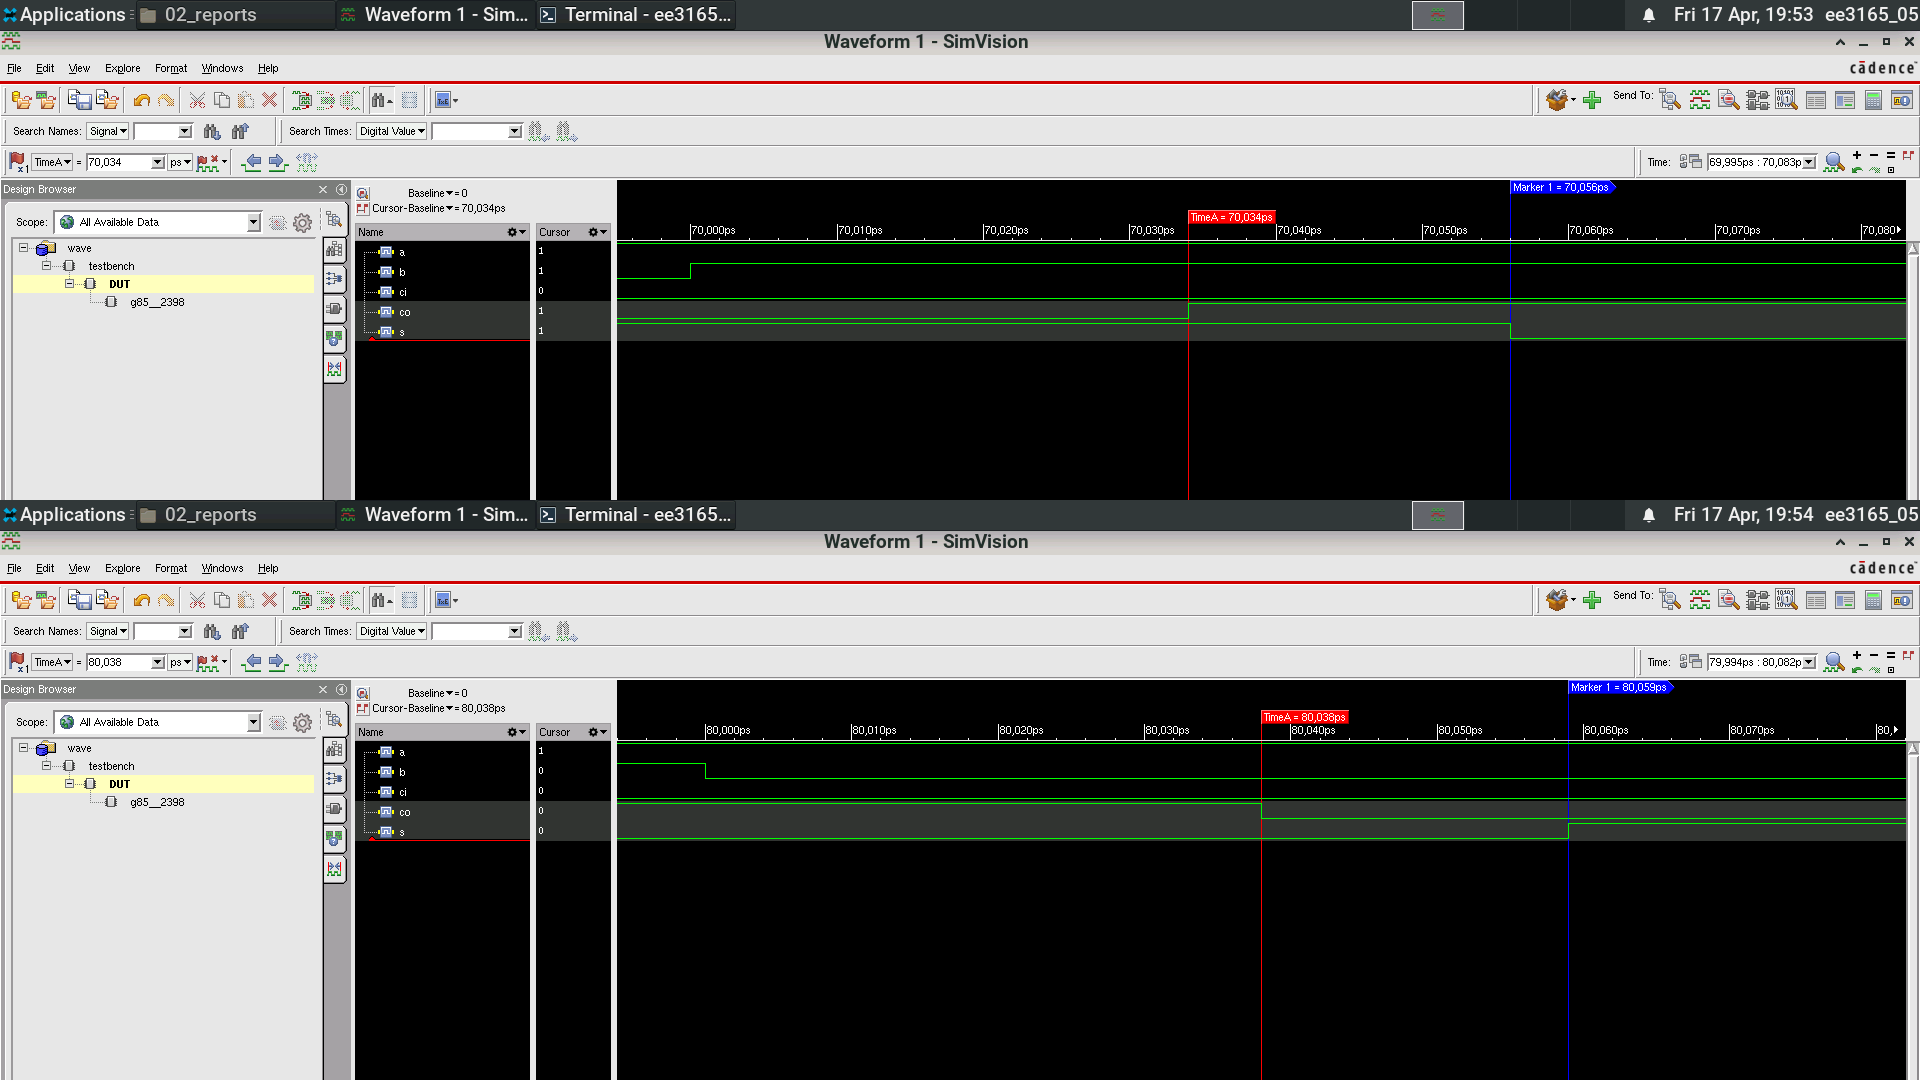
\includegraphics[width=\textwidth]{figures/fa_hvt_1v2_b_fast.png} \caption{Góc Fast} \end{subfigure} \hfill
    \begin{subfigure}[b]{0.48\textwidth} \centering 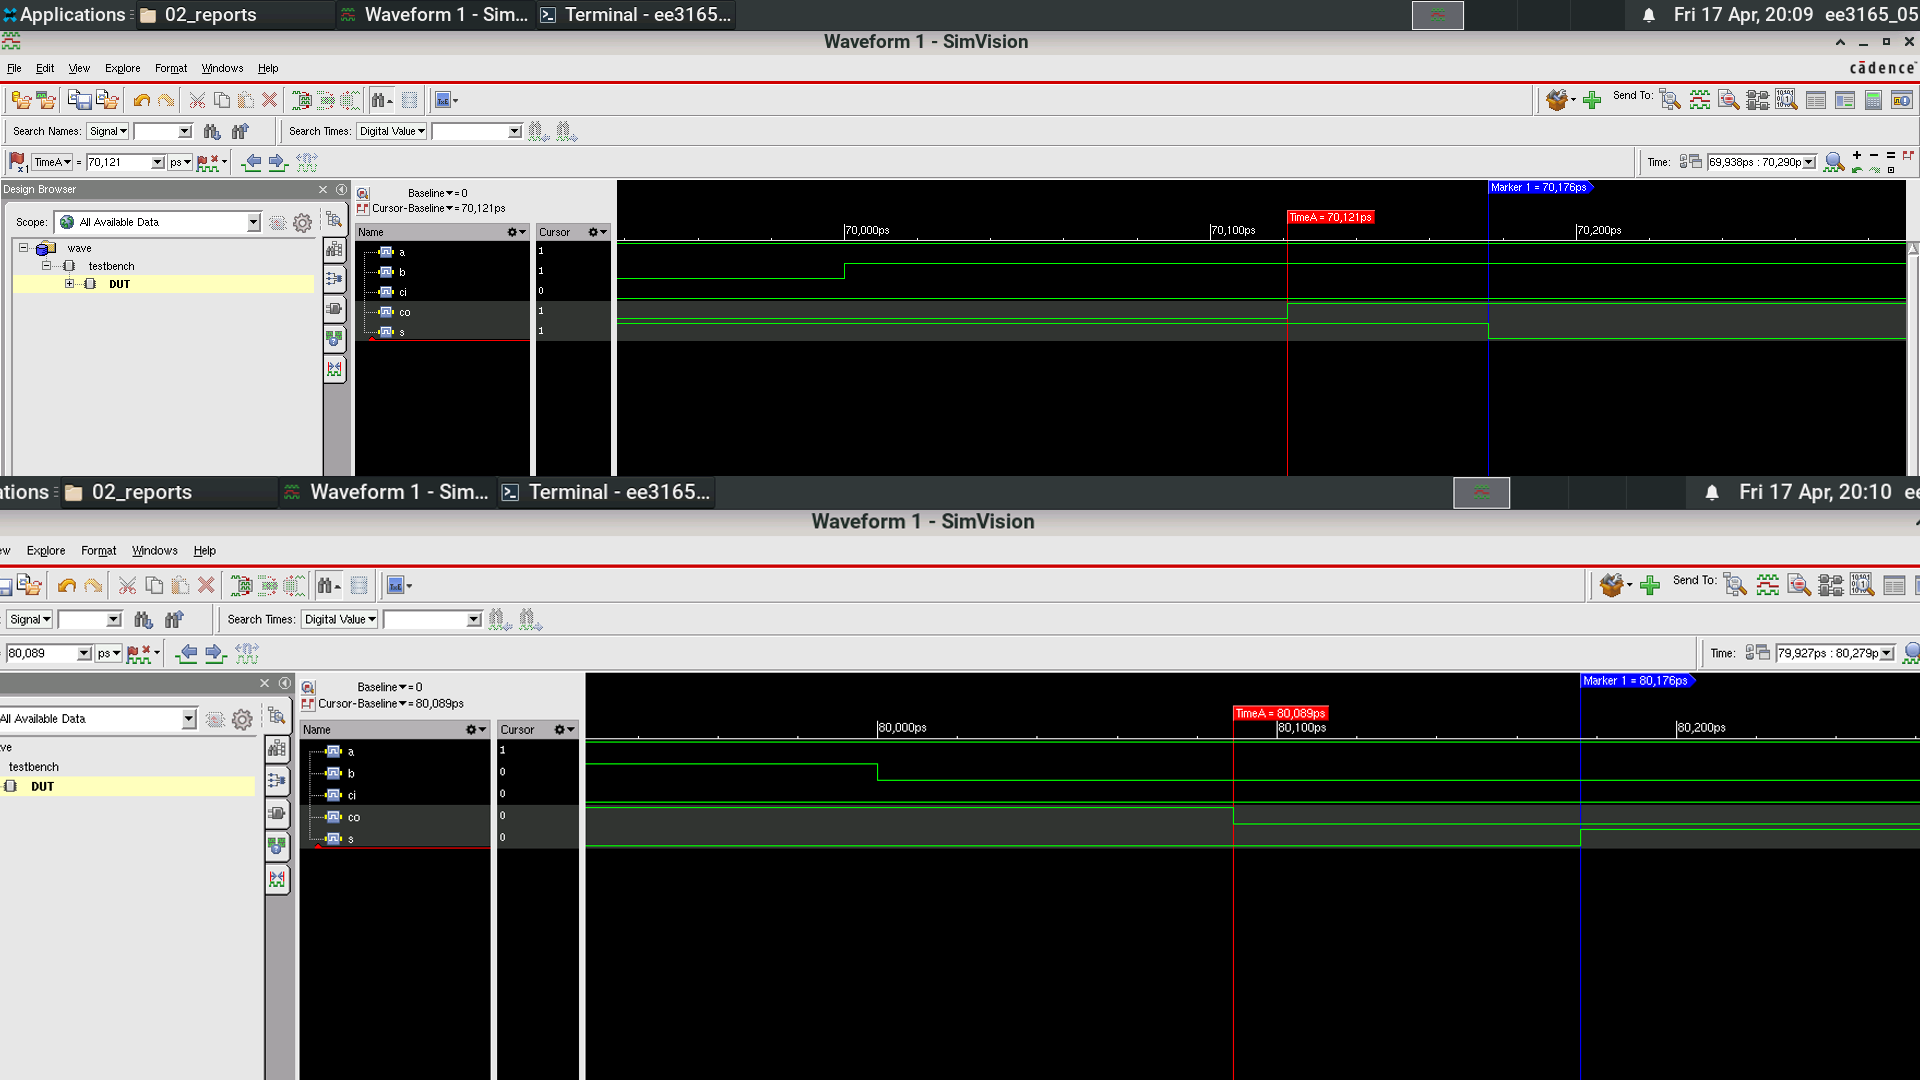
\includegraphics[width=\textwidth]{figures/fa_hvt_1v2_b_slow.png} \caption{Góc Slow} \end{subfigure}
    \caption{Dạng sóng đo độ trễ từ \textbf{B} tới các ngõ ra tại HVT 1.2V (Marker Đỏ: Cout, Xanh: Sum).}
\end{figure}

\textbf{Nhận xét (HVT - 1.2V):} Việc cấp lại mức điện áp danh định 1.2V giúp các transistor nạp xả tụ linh hoạt hơn hẳn:
\begin{itemize}
    \item \textbf{Phục hồi tốc độ chuyển mạch:} Ở góc nhanh nhất, độ trễ trên đường \texttt{Cin$\rightarrow$Cout} giảm mạnh từ 0.267 ns xuống chỉ còn 0.031 ns. Các đường dẫn ra ngõ Sum cũng được rút ngắn xuống quanh mức 0.054 ns đến 0.059 ns.
    \item \textbf{Đánh đổi công suất:} Cùng với việc tăng tốc độ, điện áp cao đẩy tổng công suất tiêu thụ tại góc nhanh nhất lên mức 1.35e-7 W, minh chứng rõ nét cho sự gia tăng của công suất động.
\end{itemize}

% ====================================================================
% KHỐI B: THƯ VIỆN LVT
% ====================================================================
\paragraph{B. Thư viện Low Threshold Voltage (LVT)}

Các cell LVT cung cấp tốc độ chuyển mạch cực nhanh nhờ giảm thiểu rào cản điện áp ngưỡng, đây là đặc tính vô giá để tăng tốc chuỗi truyền số nhớ trong bộ cộng.

\begin{table}[H]
\centering
\renewcommand{\arraystretch}{1.3}
\resizebox{\textwidth}{!}{
\begin{tabular}{|l|c|c|c|c|c|c|c|c|c|c|c|c|c|c|}
\hline
\multirow{2}{*}{\textbf{Library Name}} 
& \multirow{2}{*}{\textbf{Area}} 
& \multirow{2}{*}{\textbf{Power}} 
& \multicolumn{2}{c|}{\textbf{Cin$\rightarrow$Cout}}
& \multicolumn{2}{c|}{\textbf{A$\rightarrow$Cout}} 
& \multicolumn{2}{c|}{\textbf{B$\rightarrow$Cout}} 
& \multicolumn{2}{c|}{\textbf{Cin$\rightarrow$Sum}} 
& \multicolumn{2}{c|}{\textbf{A$\rightarrow$Sum}} 
& \multicolumn{2}{c|}{\textbf{B$\rightarrow$Sum}} \\
\cline{4-15}
& & 
& \textbf{Rise} & \textbf{Fall}
& \textbf{Rise} & \textbf{Fall}
& \textbf{Rise} & \textbf{Fall}
& \textbf{Rise} & \textbf{Fall}
& \textbf{Rise} & \textbf{Fall}
& \textbf{Rise} & \textbf{Fall} \\
\hline
fast\_vdd1v0\_basicCells\_lvt 
& 5.130 & 1.13149e-07 & 0.026 & 0.030 & 0.027 & 0.032 & 0.028 & 0.031 & 0.047 & 0.044 & 0.047 & 0.047 & 0.048 & 0.046 \\ \hline
fast\_vdd1v2\_basicCells\_lvt 
& 5.130 & 1.64422e-07 & 0.020 & 0.024 & 0.022 & 0.026 & 0.022 & 0.025 & 0.038 & 0.036 & 0.038 & 0.037 & 0.038 & 0.037 \\ \hline
slow\_vdd1v0\_basicCells\_lvt 
& 5.130 & 6.44167e-08 & 0.100 & 0.092 & 0.109 & 0.094 & 0.108 & 0.094 & 0.166 & 0.154 & 0.163 & 0.171 & 0.170 & 0.168 \\ \hline
slow\_vdd1v2\_basicCells\_lvt 
& 5.130 & 9.90057e-08 & 0.062 & 0.059 & 0.068 & 0.062 & 0.068 & 0.061 & 0.106 & 0.097 & 0.104 & 0.107 & 0.108 & 0.106 \\ \hline
\end{tabular}
}
\caption{Tổng hợp thông số Area, Power và Delay 6 đường dẫn của Full Adder (LVT).}
\label{tab:exp1_fa_lvt_params}
\end{table}

\textbf{1. Khảo sát LVT tại điện áp thấp (VDD = 1.0V)}

\begin{figure}[H] \centering
    \begin{subfigure}[b]{0.48\textwidth} \centering 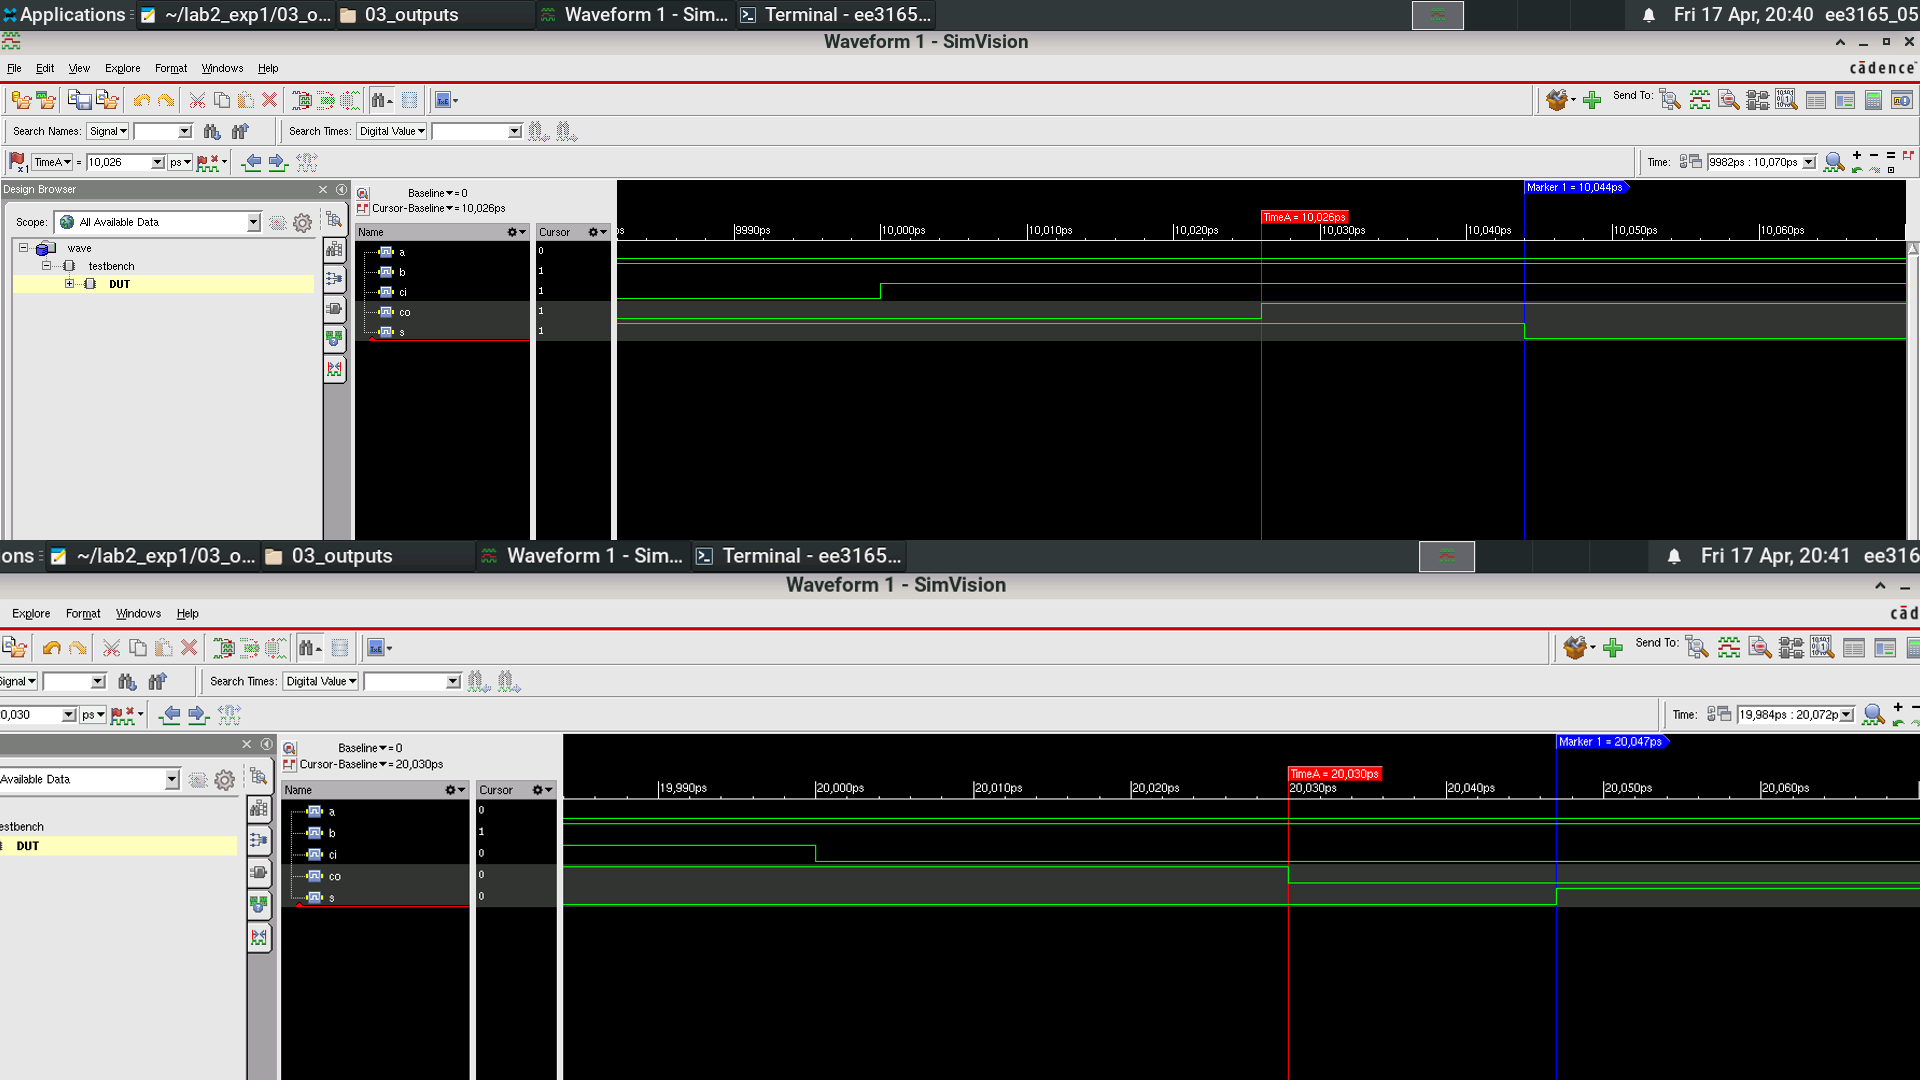
\includegraphics[width=\textwidth]{figures/fa_lvt_1v0_cin_fast.png} \caption{Góc Fast} \end{subfigure} \hfill
    \begin{subfigure}[b]{0.48\textwidth} \centering 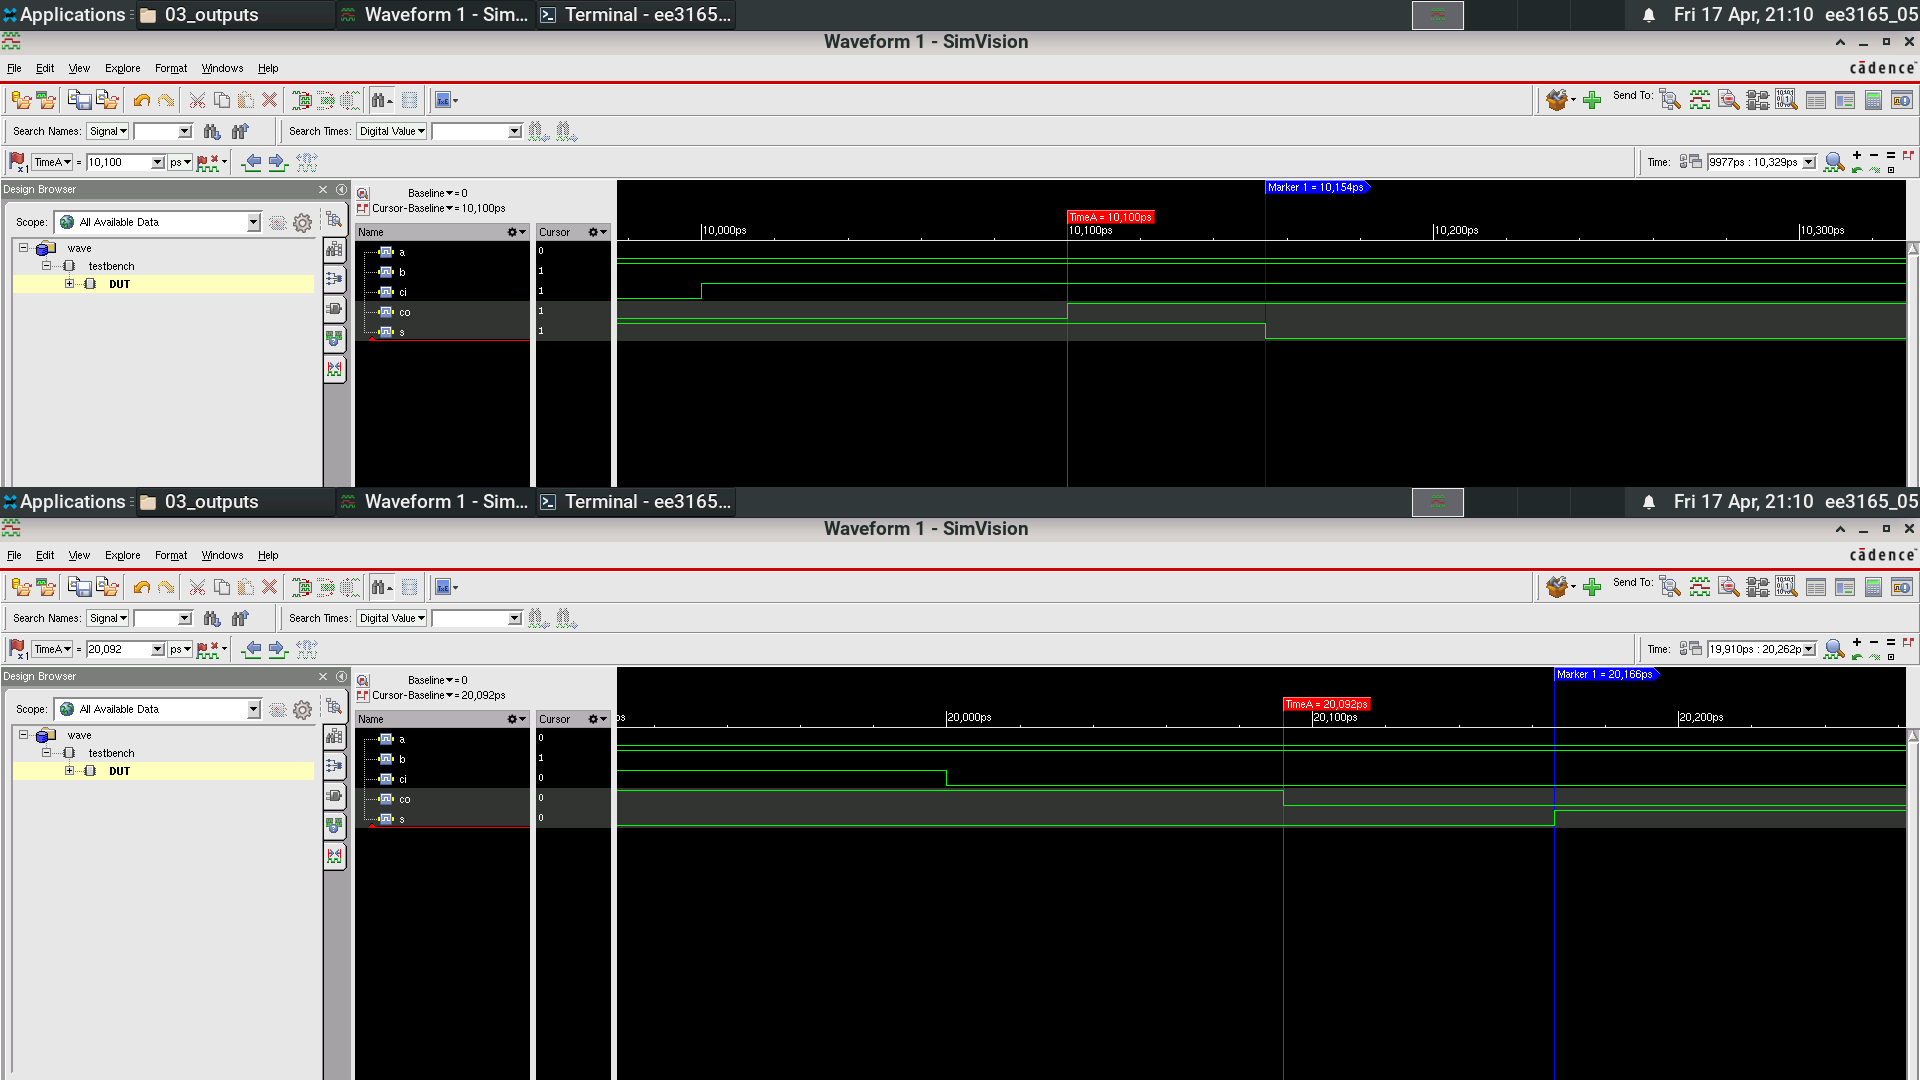
\includegraphics[width=\textwidth]{figures/fa_lvt_1v0_cin_slow.png} \caption{Góc Slow} \end{subfigure}
    \caption{Dạng sóng đo độ trễ từ \textbf{Cin} tới các ngõ ra tại LVT 1.0V (Marker Đỏ: Cout, Xanh: Sum).}
\end{figure}

\begin{figure}[H] \centering
    \begin{subfigure}[b]{0.48\textwidth} \centering 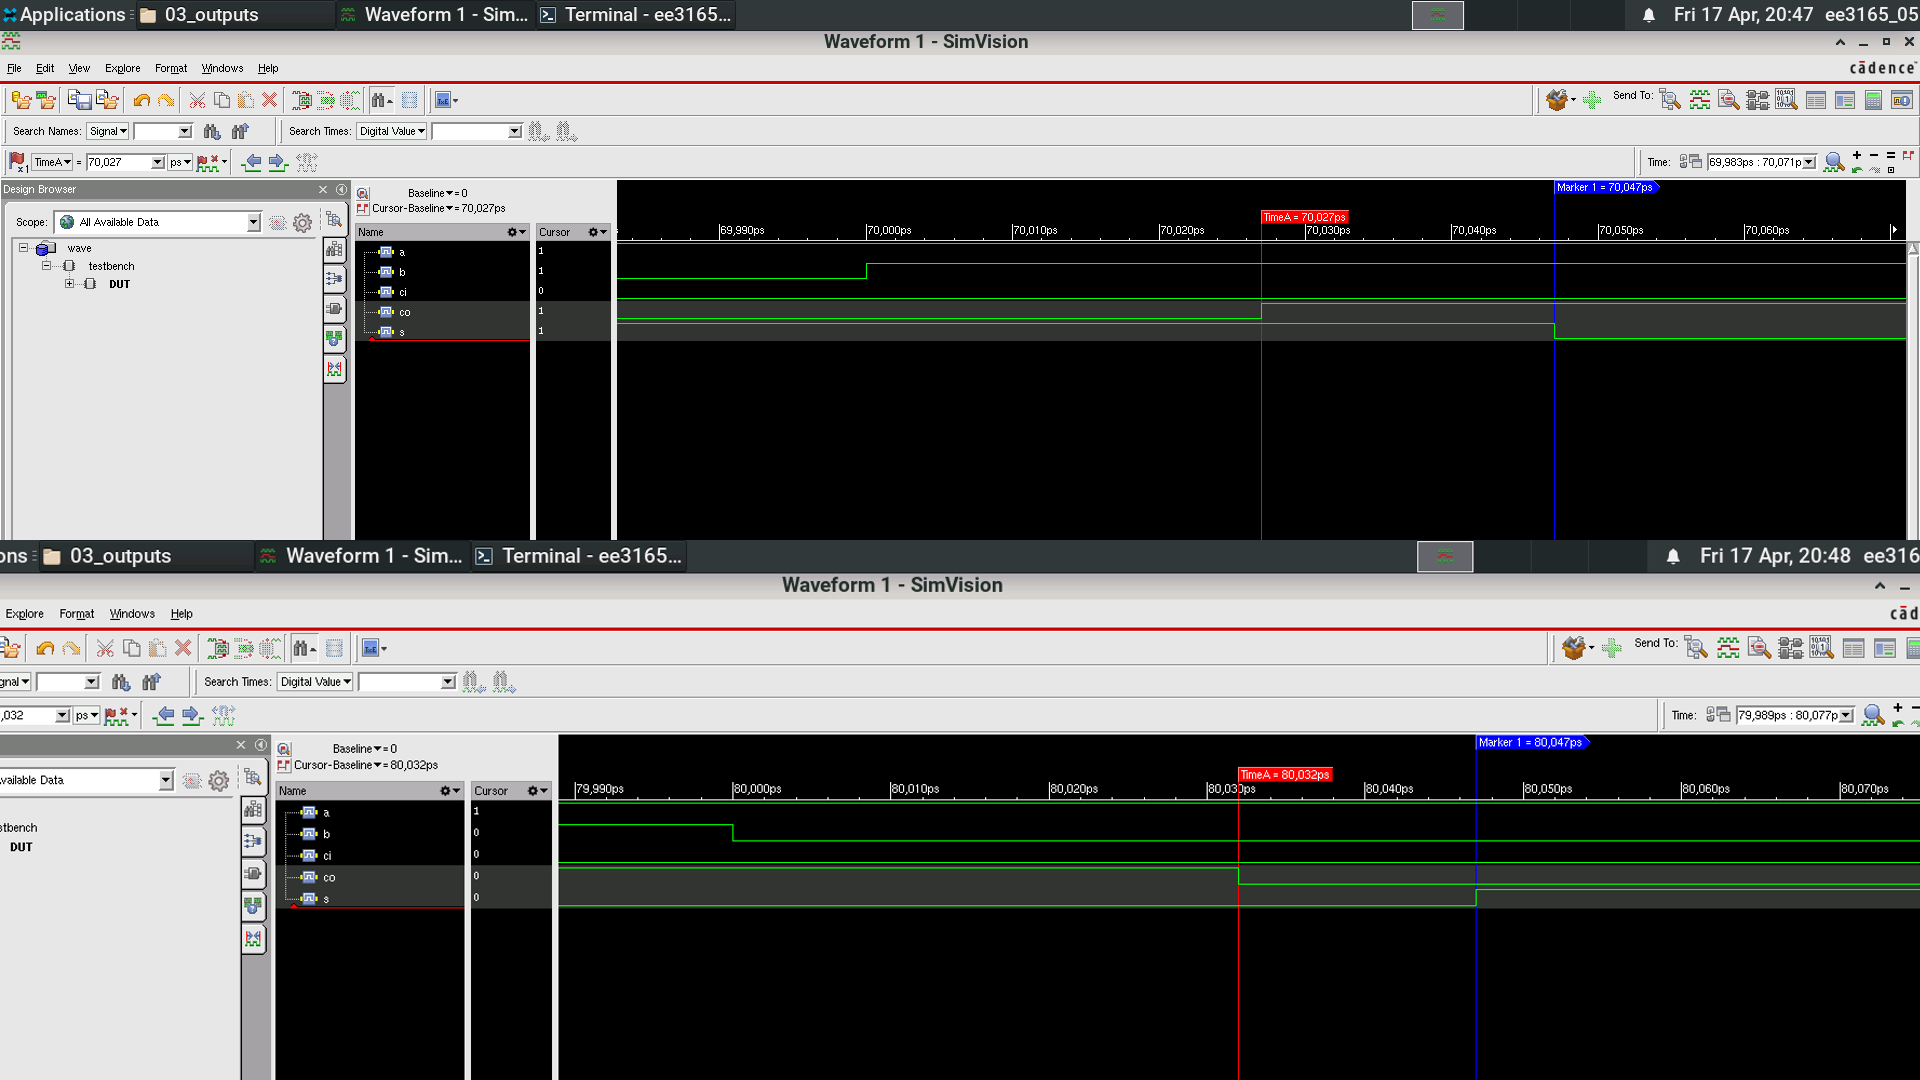
\includegraphics[width=\textwidth]{figures/fa_lvt_1v0_a_fast.png} \caption{Góc Fast} \end{subfigure} \hfill
    \begin{subfigure}[b]{0.48\textwidth} \centering 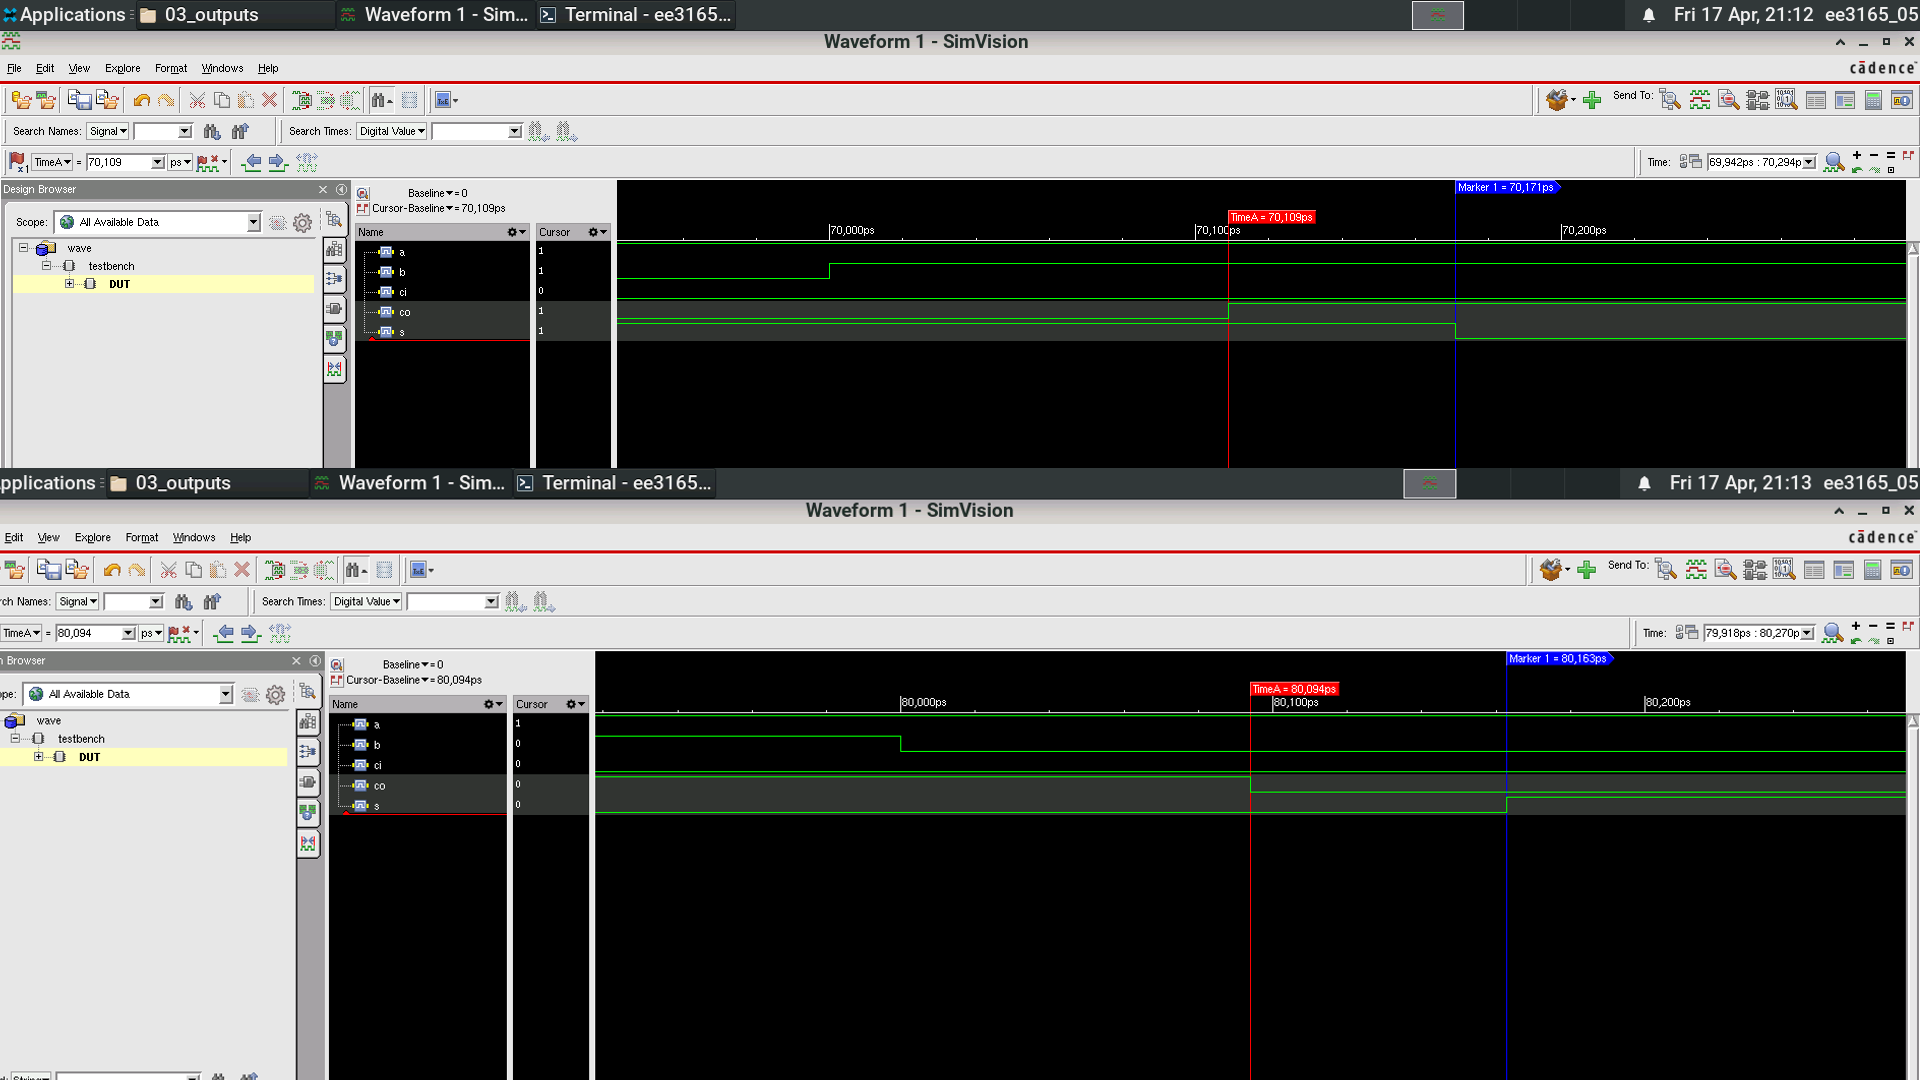
\includegraphics[width=\textwidth]{figures/fa_lvt_1v0_a_slow.png} \caption{Góc Slow} \end{subfigure}
    \caption{Dạng sóng đo độ trễ từ \textbf{A} tới các ngõ ra tại LVT 1.0V (Marker Đỏ: Cout, Xanh: Sum).}
\end{figure}

\begin{figure}[H] \centering
    \begin{subfigure}[b]{0.48\textwidth} \centering 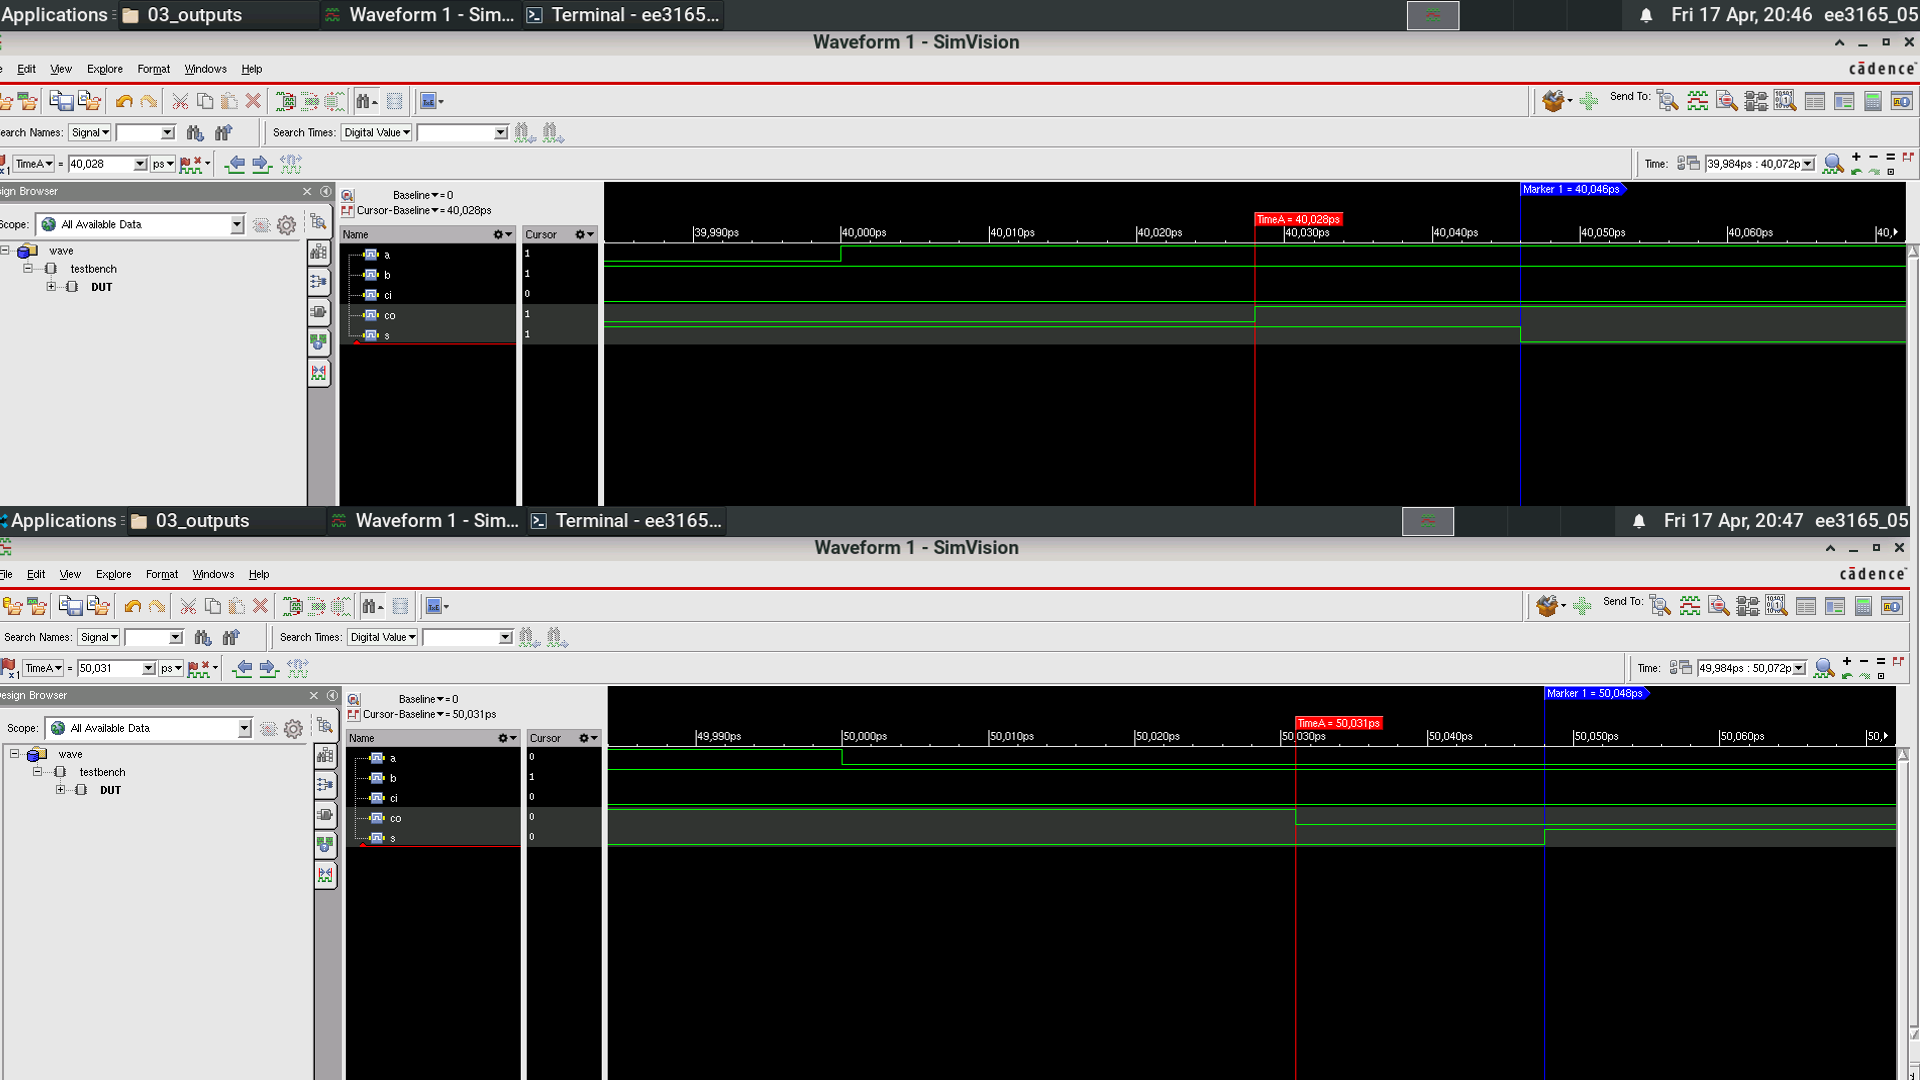
\includegraphics[width=\textwidth]{figures/fa_lvt_1v0_b_fast.png} \caption{Góc Fast} \end{subfigure} \hfill
    \begin{subfigure}[b]{0.48\textwidth} \centering 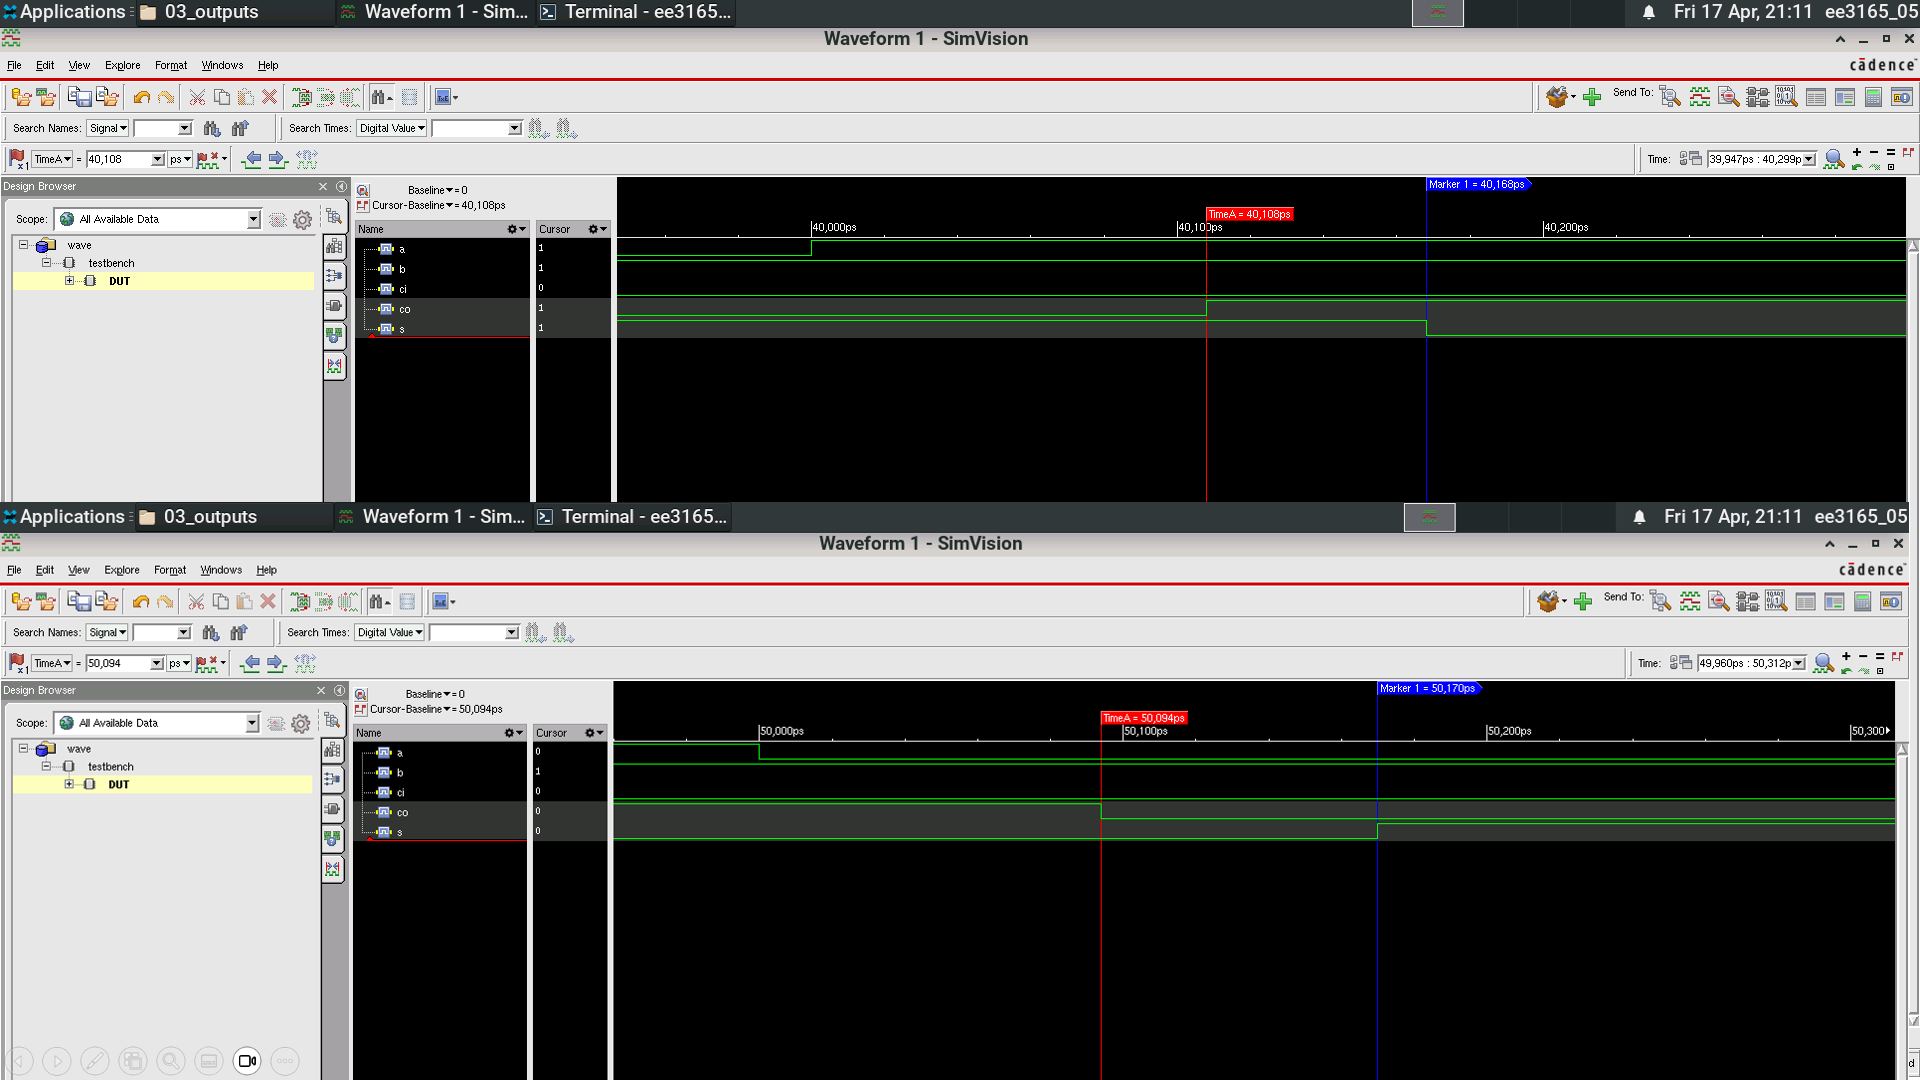
\includegraphics[width=\textwidth]{figures/fa_lvt_1v0_b_slow.png} \caption{Góc Slow} \end{subfigure}
    \caption{Dạng sóng đo độ trễ từ \textbf{B} tới các ngõ ra tại LVT 1.0V (Marker Đỏ: Cout, Xanh: Sum).}
\end{figure}

\textbf{Nhận xét (LVT - 1.0V):} Khi hệ thống bắt buộc phải hạ áp để tiết kiệm năng lượng, thư viện LVT phát huy tác dụng bù đắp vô cùng hiệu quả:
\begin{itemize}
    \item \textbf{Giải quyết điểm nghẽn thời gian:} So với góc chậm nhất của HVT (0.267 ns), linh kiện LVT đã kéo giảm độ trễ sườn lên của đường \texttt{Cin$\rightarrow$Cout} xuống chỉ còn 0.100 ns. Tương tự, đường \texttt{A$\rightarrow$Sum} cũng giảm từ 0.418 ns xuống 0.163 ns. Điều này giúp khối cộng duy trì được tần số hoạt động ổn định bất chấp nguồn điện suy giảm.
    \item \textbf{Gia tăng công suất tĩnh:} Sự cải thiện về tốc độ phải đánh đổi bằng mức tiêu thụ 6.44e-8 W ở góc chậm nhất, do đặc tính dòng rò dưới ngưỡng của linh kiện LVT luôn cao hơn HVT.
\end{itemize}

\textbf{2. Khảo sát LVT tại điện áp danh định (VDD = 1.2V)}

\begin{figure}[H] \centering
    \begin{subfigure}[b]{0.48\textwidth} \centering 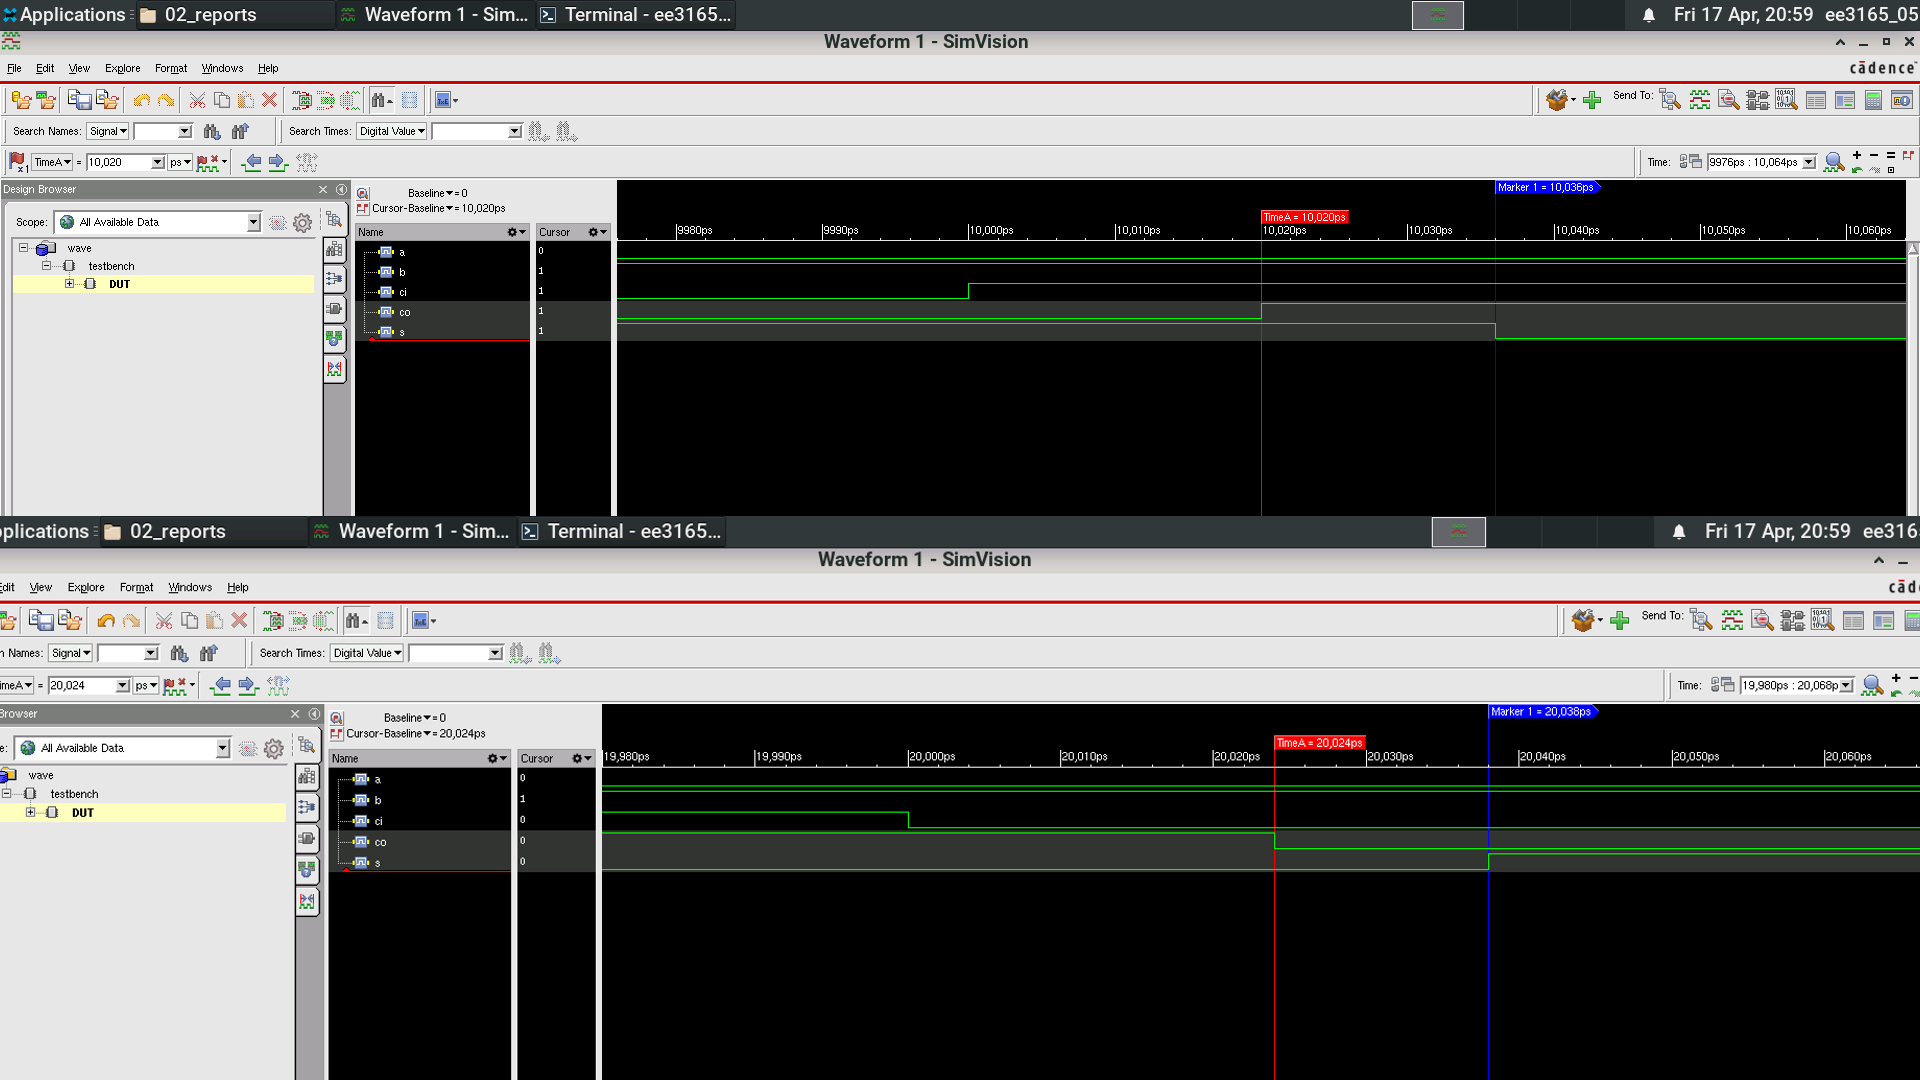
\includegraphics[width=\textwidth]{figures/fa_lvt_1v2_cin_fast.png} \caption{Góc Fast} \end{subfigure} \hfill
    \begin{subfigure}[b]{0.48\textwidth} \centering 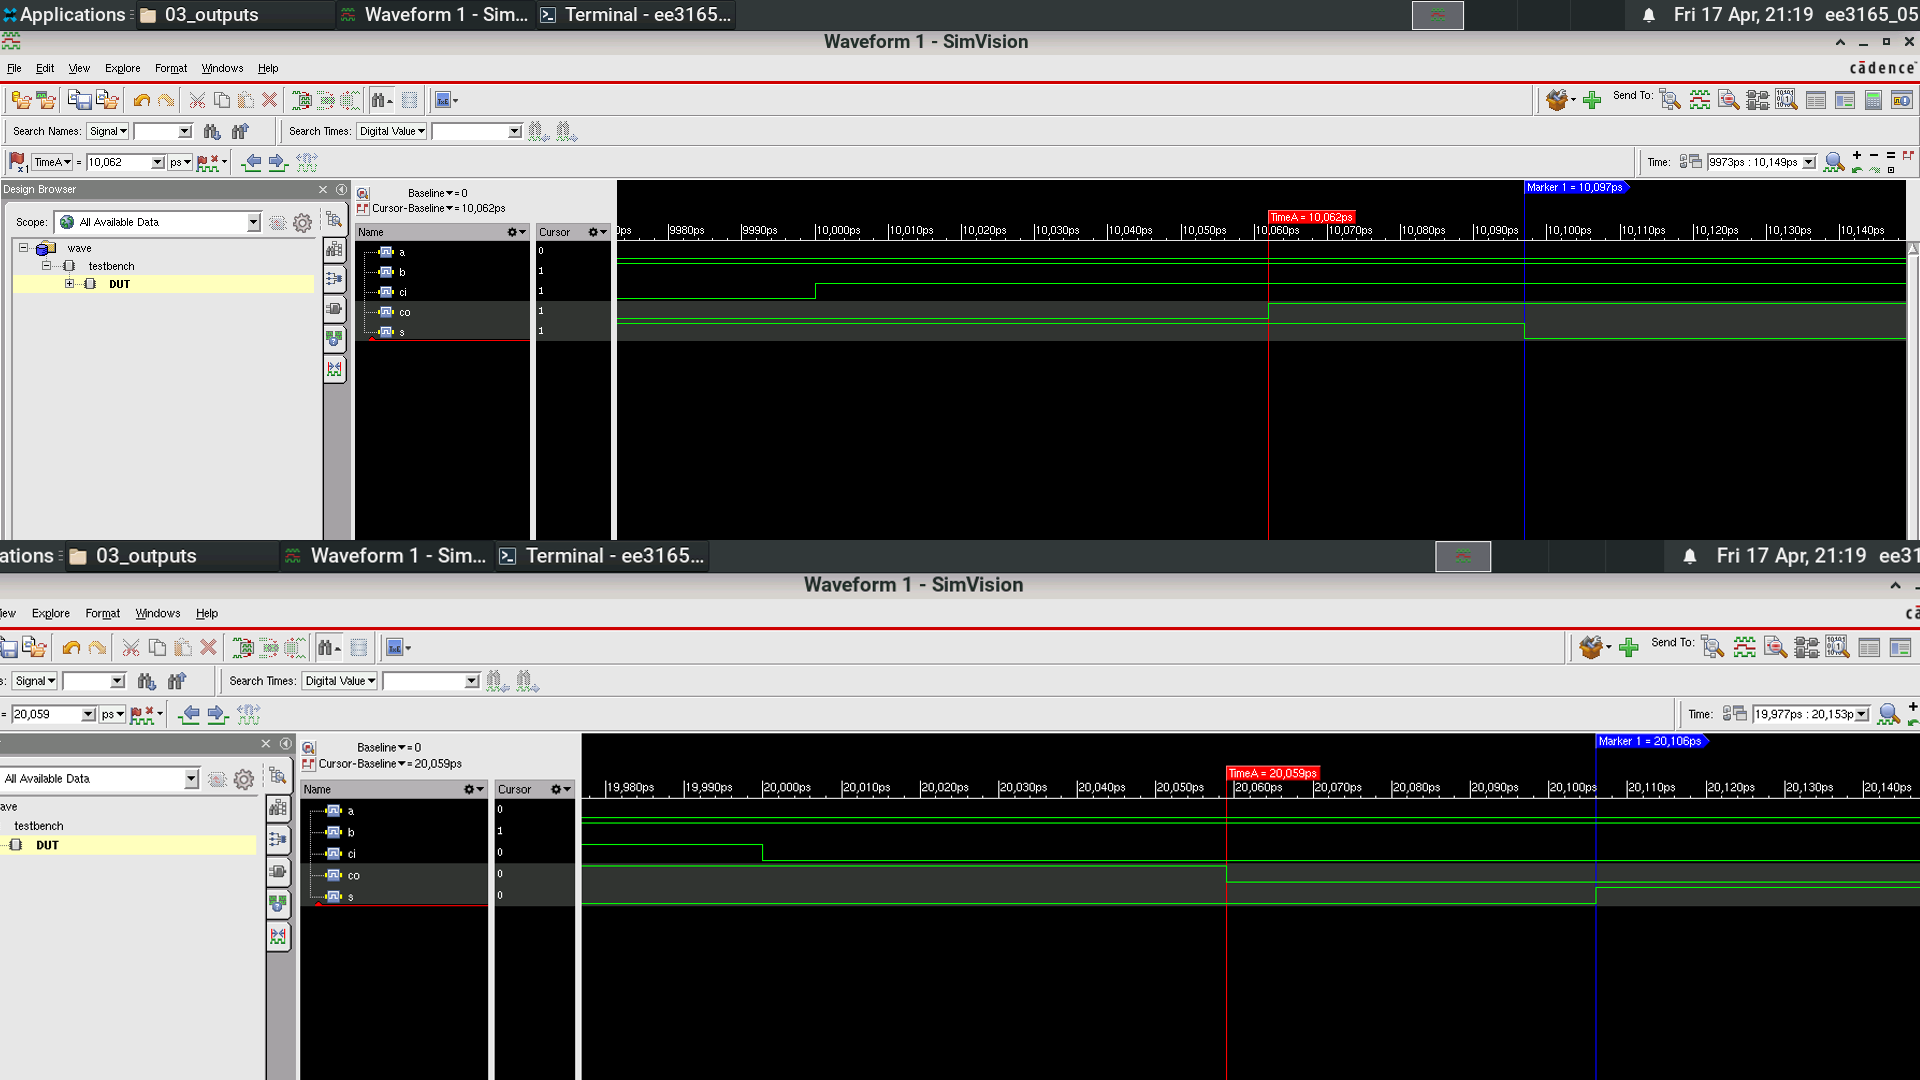
\includegraphics[width=\textwidth]{figures/fa_lvt_1v2_cin_slow.png} \caption{Góc Slow} \end{subfigure}
    \caption{Dạng sóng đo độ trễ từ \textbf{Cin} tới các ngõ ra tại LVT 1.2V (Marker Đỏ: Cout, Xanh: Sum).}
\end{figure}

\begin{figure}[H] \centering
    \begin{subfigure}[b]{0.48\textwidth} \centering 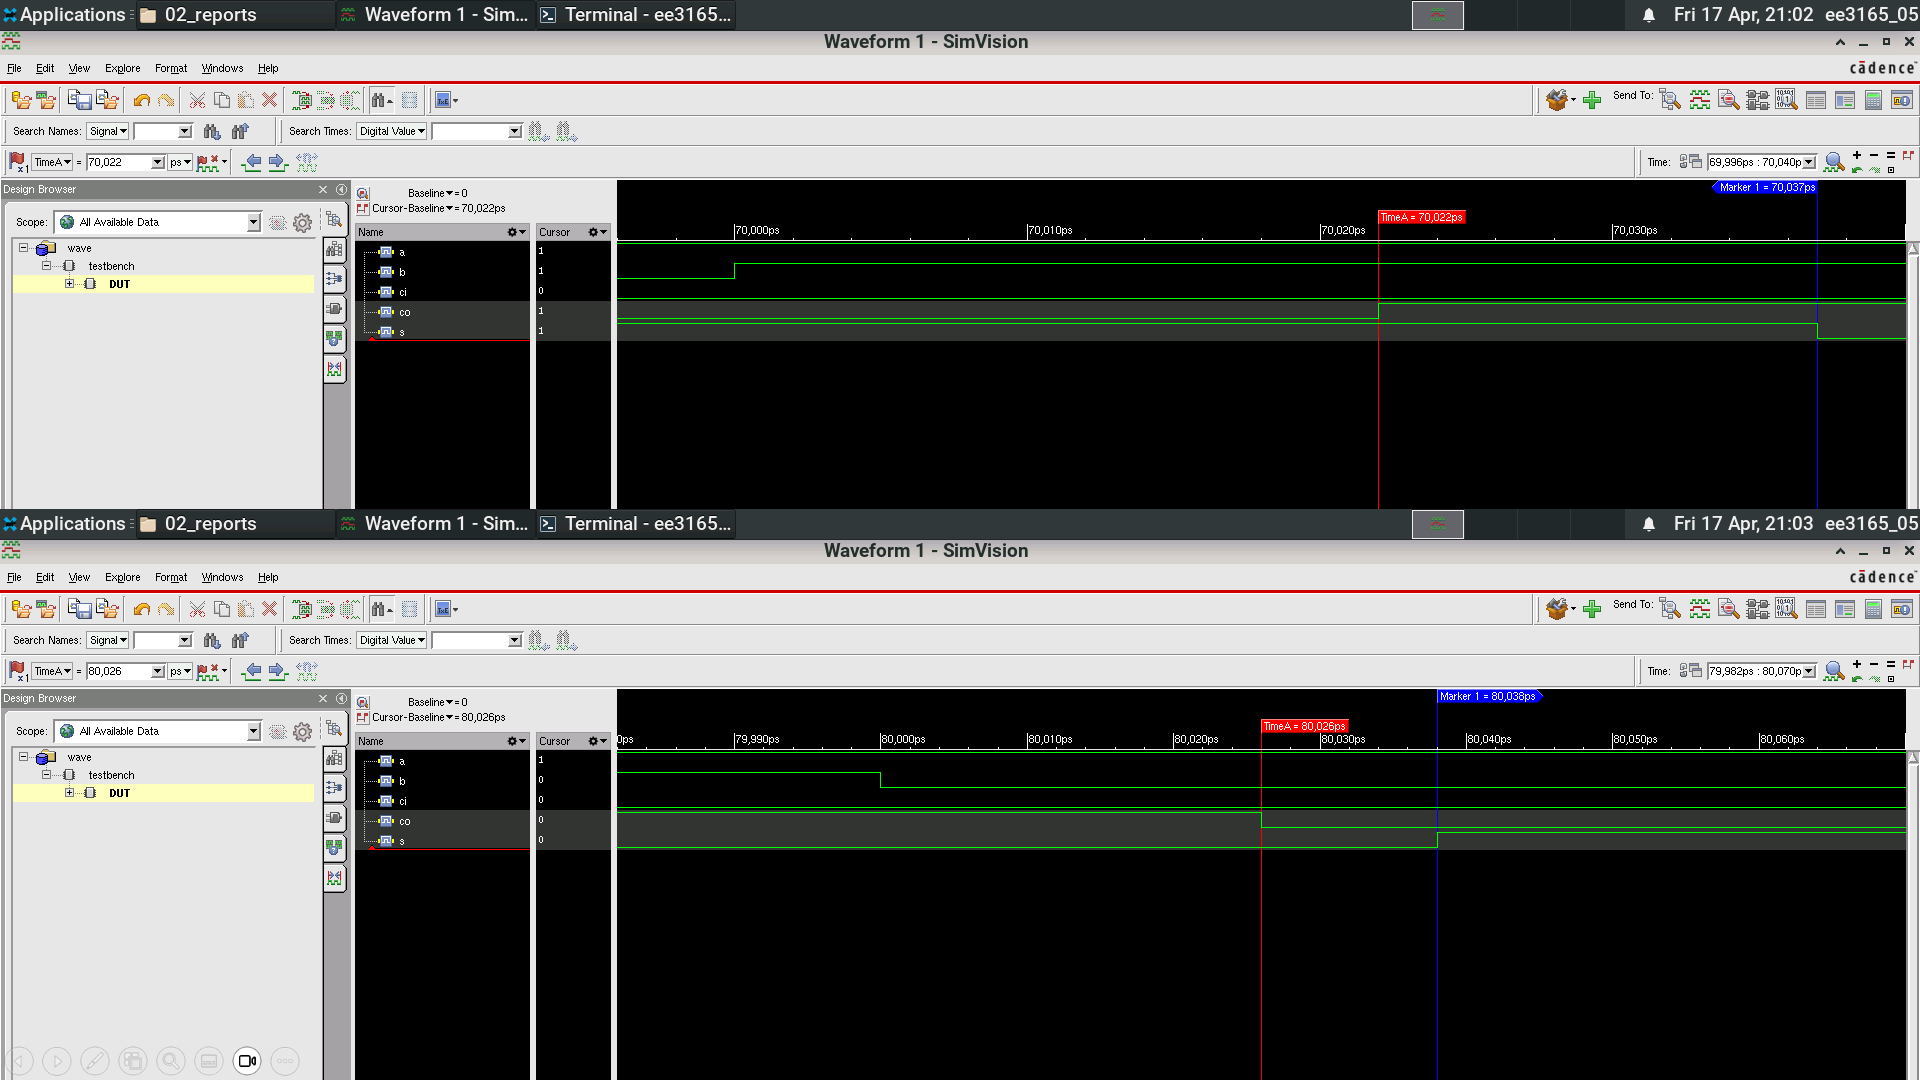
\includegraphics[width=\textwidth]{figures/fa_lvt_1v2_a_fast.png} \caption{Góc Fast} \end{subfigure} \hfill
    \begin{subfigure}[b]{0.48\textwidth} \centering 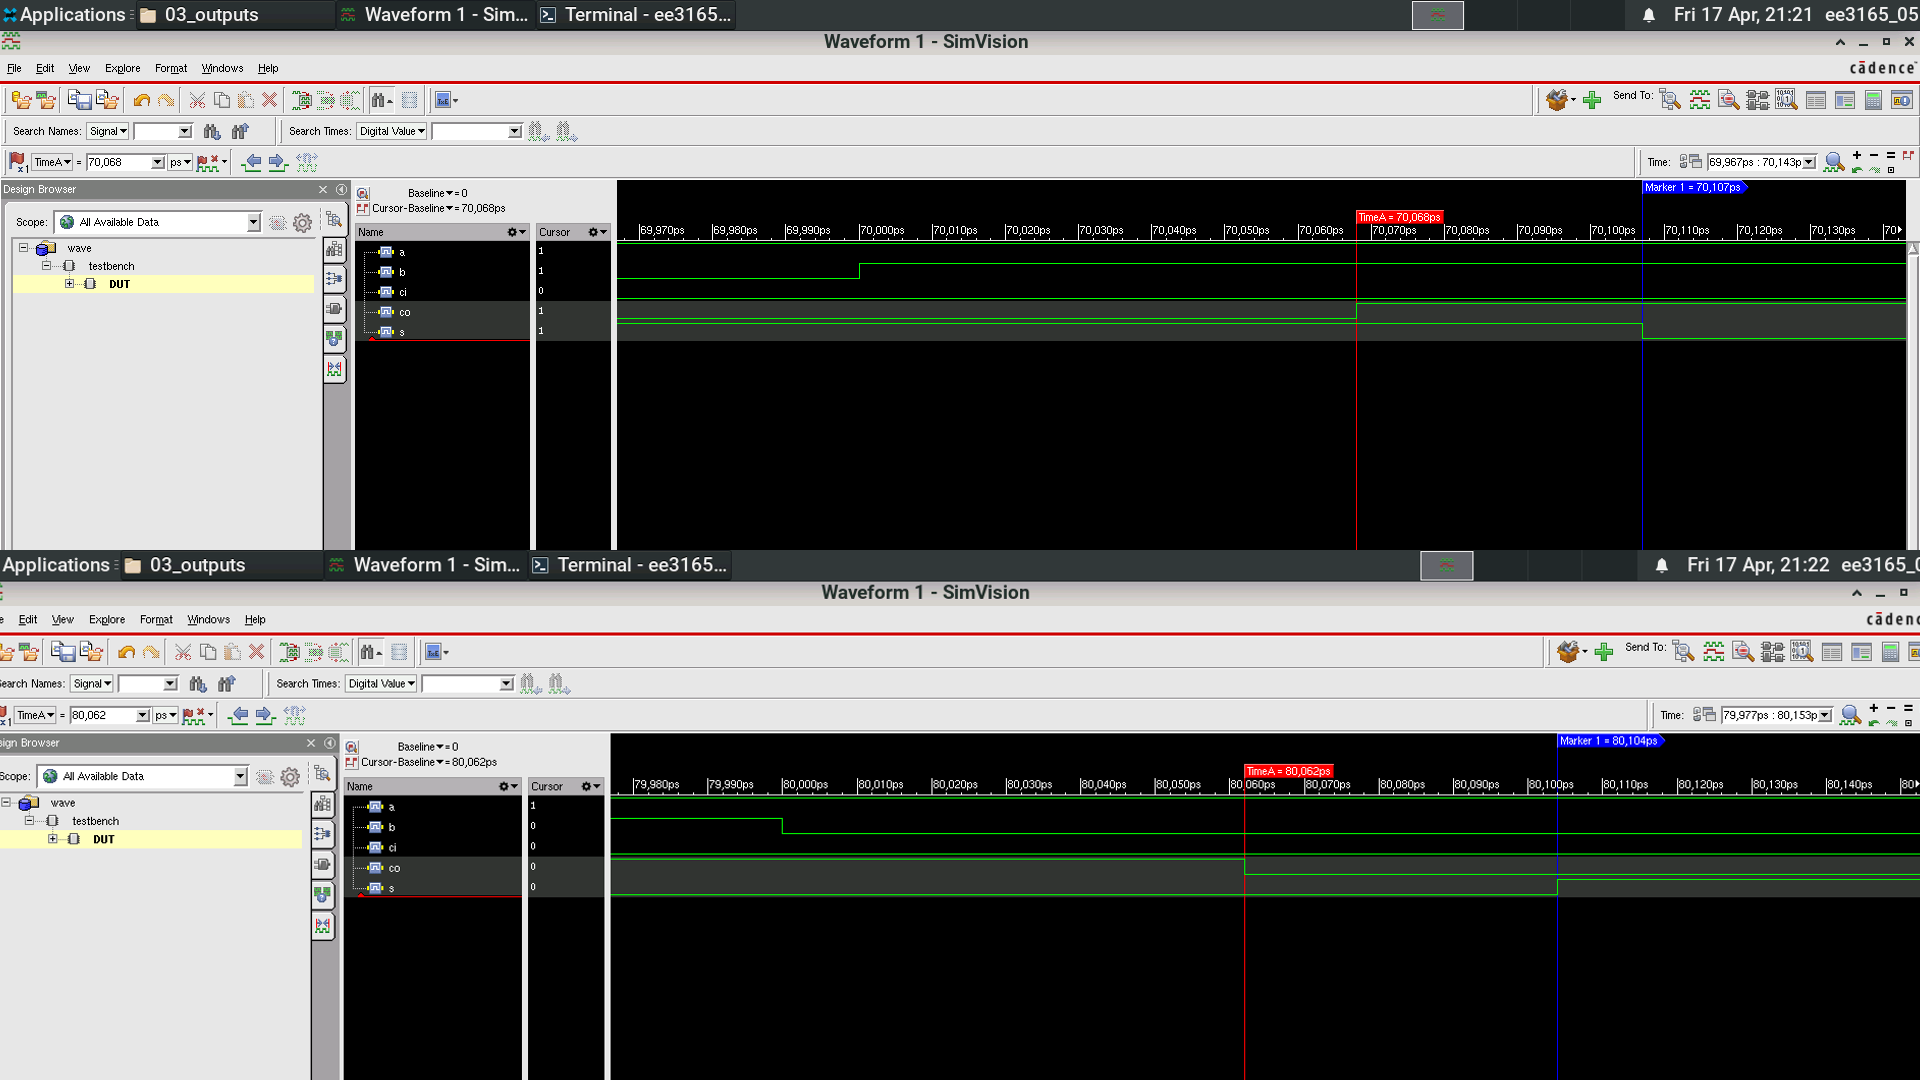
\includegraphics[width=\textwidth]{figures/fa_lvt_1v2_a_slow.png} \caption{Góc Slow} \end{subfigure}
    \caption{Dạng sóng đo độ trễ từ \textbf{A} tới các ngõ ra tại LVT 1.2V (Marker Đỏ: Cout, Xanh: Sum).}
\end{figure}

\begin{figure}[H] \centering
    \begin{subfigure}[b]{0.48\textwidth} \centering 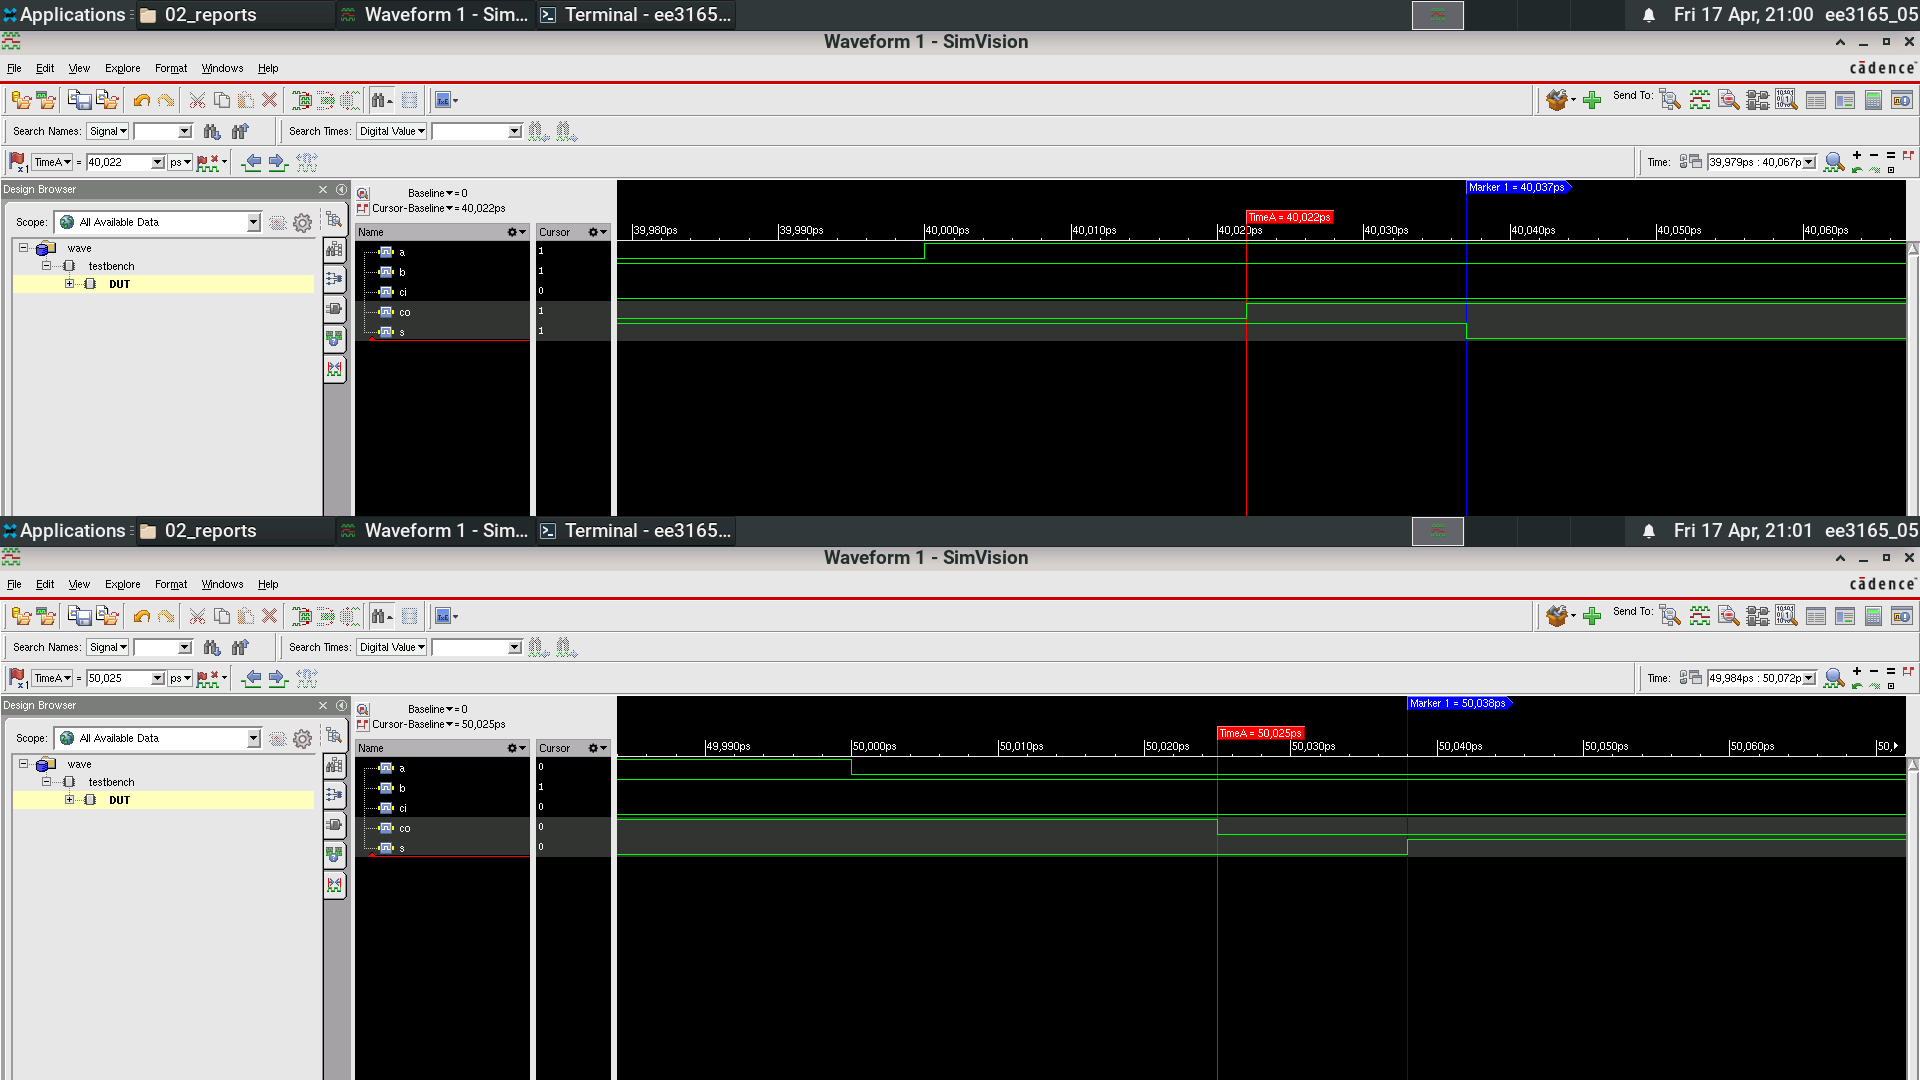
\includegraphics[width=\textwidth]{figures/fa_lvt_1v2_b_fast.png} \caption{Góc Fast} \end{subfigure} \hfill
    \begin{subfigure}[b]{0.48\textwidth} \centering 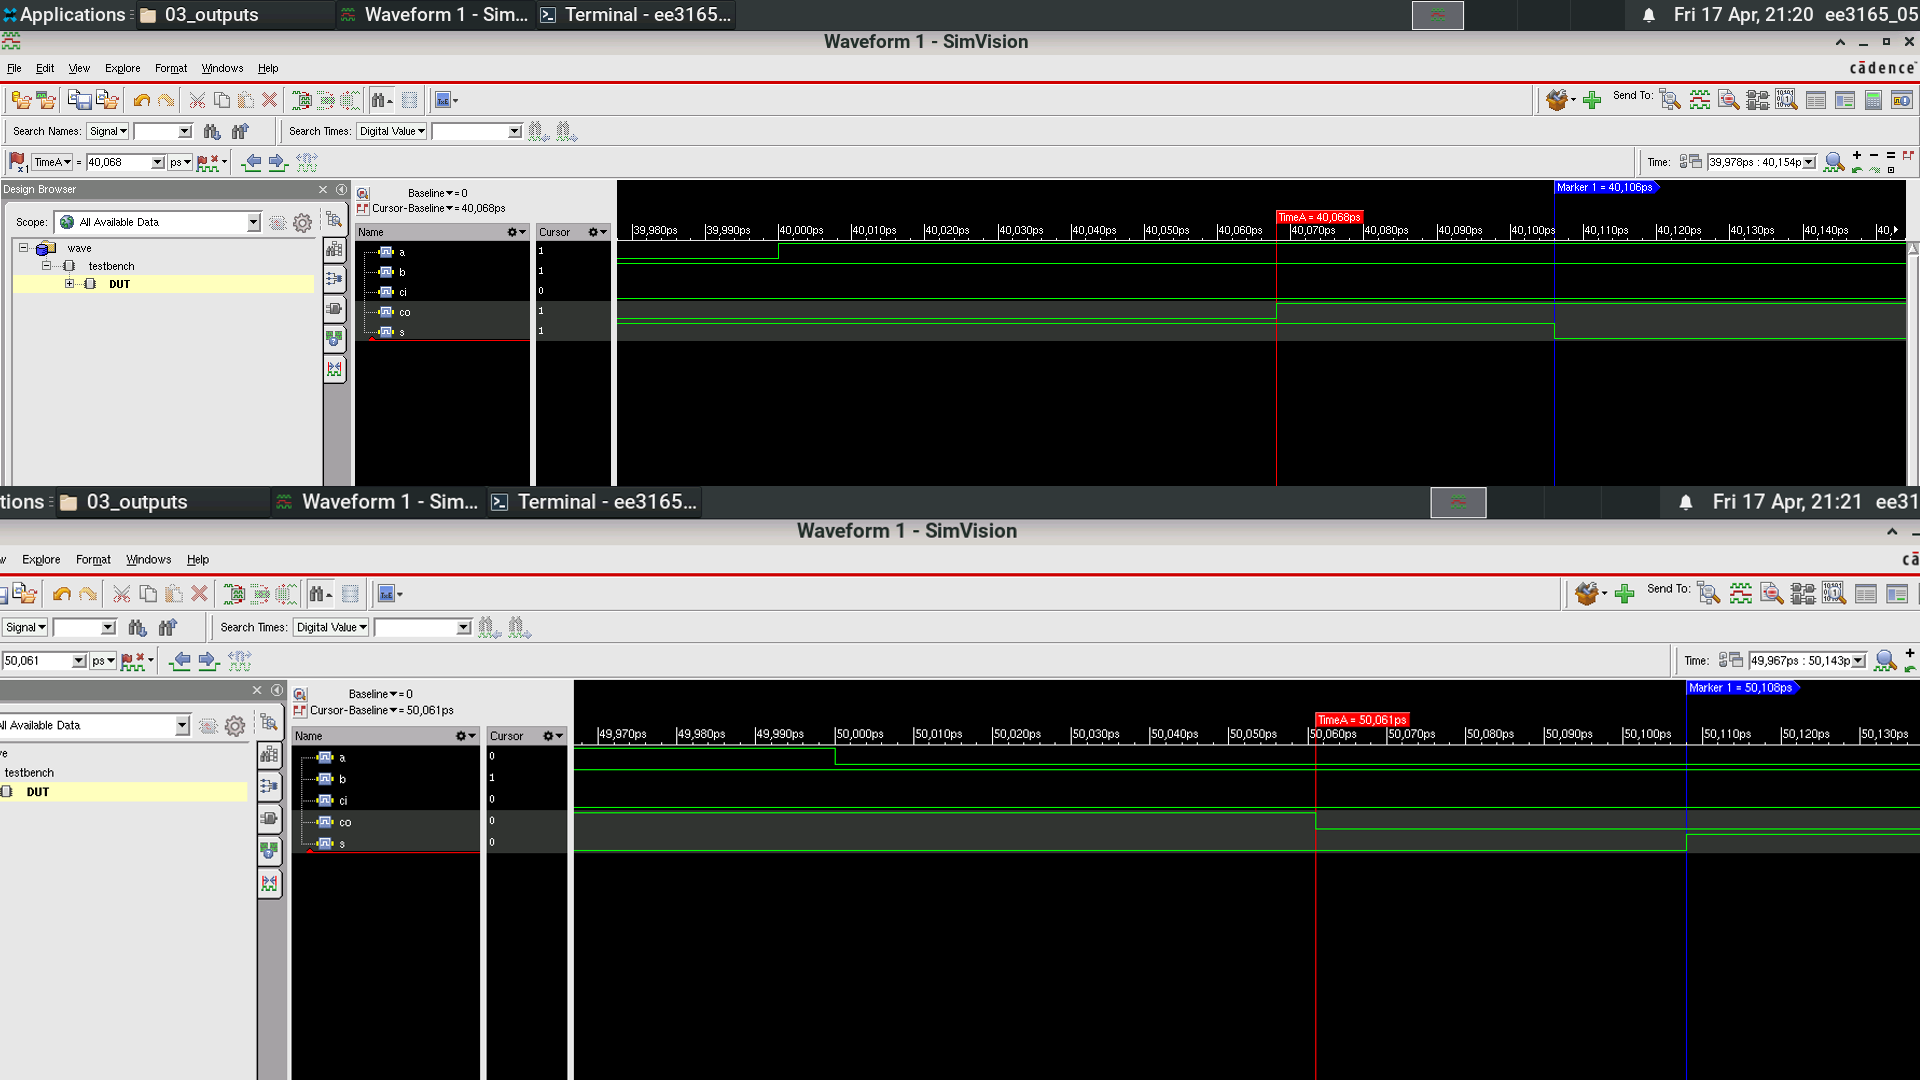
\includegraphics[width=\textwidth]{figures/fa_lvt_1v2_b_slow.png} \caption{Góc Slow} \end{subfigure}
    \caption{Dạng sóng đo độ trễ từ \textbf{B} tới các ngõ ra tại LVT 1.2V (Marker Đỏ: Cout, Xanh: Sum).}
\end{figure}

\textbf{Nhận xét (LVT - 1.2V):} 
\begin{itemize}
    \item \textbf{Hiệu năng cực đại:} Tại góc vận hành lý tưởng nhất, khối cộng loại bỏ hoàn toàn hiện tượng suy hao sườn xung. Đường truyền số nhớ \texttt{Cin$\rightarrow$Cout} chỉ mất 0.020 ns để phản hồi, đáp ứng xuất sắc cho các hệ thống vi xử lý yêu cầu xung nhịp vô cùng khắt khe.
    \item \textbf{Đỉnh điểm tiêu thụ điện:} Đây là cấu hình tiêu tốn năng lượng nhất toàn bài thí nghiệm với công suất tổng cộng lên tới 1.64e-7 W. Việc sử dụng bừa bãi linh kiện này sẽ dễ dàng dẫn đến các vấn đề nghiêm trọng về quản lý nhiệt độ.
\end{itemize}

\paragraph{C. Kết luận} 
Phân tích khối cộng toàn phần làm rõ đặc tính độ trễ phụ thuộc đường dẫn trong các mạch tổ hợp phức tạp. Dù diện tích luôn cố định ở 5.130 $\mu m^2$, sự chênh lệch thời gian giữa ngõ ra \texttt{Sum} và \texttt{Cout} là rất lớn do khác biệt về độ sâu logic. Trong thực tế thiết kế vi mạch, đường truyền số nhớ \texttt{Cin$\rightarrow$Cout} luôn là đường dẫn tới hạn quyết định tốc độ của toàn hệ thống. Do đó, giải pháp tối ưu hóa điện năng và tốc độ hiệu quả nhất là sử dụng thư viện LVT riêng cho các đường tạo số nhớ \texttt{Cout} để tăng tốc, đồng thời giữ các nhánh tạo tổng \texttt{Sum} ở dạng HVT để kìm hãm công suất rò rỉ.

\subsection{Area parameters}

Bảng dưới đây thống kê diện tích của 6 standard cells bao gồm NOT, OR2, NAND2, NOR2, MUX, và FULL ADDER qua 8 process corners.

\begin{table}[H]
    \centering
    \begin{tabular}{|l|c|c|c|c|c|c|}
        \hline
        \textbf{Process Corner (VDD, Vth)} & \textbf{NOT} & \textbf{OR2} & \textbf{NAND2} & \textbf{NOR2} & \textbf{MUX} & \textbf{FA} \\
        \hline
        Fast (FF), 1.0V, HVT & 0.684 & 1.368 & 1.026 & 1.026 & 2.394 & 5.130 \\ \hline
        Fast (FF), 1.2V, HVT & 0.684 & 1.368 & 1.026 & 1.026 & 2.394 & 5.130 \\ \hline
        Slow (SS), 1.0V, HVT & 0.684 & 1.368 & 1.026 & 1.026 & 2.394 & 5.130 \\ \hline
        Slow (SS), 1.2V, HVT & 0.684 & 1.368 & 1.026 & 1.026 & 2.394 & 5.130 \\ \hline
        Fast (FF), 1.0V, LVT & 0.684 & 1.368 & 1.026 & 1.026 & 2.394 & 5.130 \\ \hline
        Fast (FF), 1.2V, LVT & 0.684 & 1.368 & 1.026 & 1.026 & 2.394 & 5.130 \\ \hline
        Slow (SS), 1.0V, LVT & 0.684 & 1.368 & 1.026 & 1.026 & 2.394 & 5.130 \\ \hline
        Slow (SS), 1.2V, LVT & 0.684 & 1.368 & 1.026 & 1.026 & 2.394 & 5.130 \\ \hline
    \end{tabular}
    \caption{Area parameters ($\mu m^2$) của các cells qua 8 corners}
    \label{tab:exp1_area}
\end{table}

%--------------------------------------------------
\subsection{Power parameters}

Bảng dưới đây thống kê công suất tổng tiêu thụ của các cells qua 8 process corners. Số liệu được quy đổi sang đơn vị nanoWatt (nW) để thuận tiện cho việc so sánh.

\begin{table}[H]
    \centering
    \resizebox{\textwidth}{!}{
    \begin{tabular}{|l|c|c|c|c|c|c|}
        \hline
        \textbf{Process Corner (VDD, Vth)} & \textbf{NOT} & \textbf{OR2} & \textbf{NAND2} & \textbf{NOR2} & \textbf{MUX} & \textbf{FA} \\
        \hline
        Fast (FF), 1.0V, HVT & 5.93 & 17.37 & 10.60 & 10.75 & 36.59 & 87.21 \\ \hline
        Fast (FF), 1.2V, HVT & 8.61 & 25.32 & 15.41 & 15.66 & 54.70 & 135.37 \\ \hline
        Slow (SS), 1.0V, HVT & 3.99 & 11.47 & 7.21 & 7.31 & 23.96 & 53.70 \\ \hline
        Slow (SS), 1.2V, HVT & 5.82 & 16.88 & 10.47 & 10.65 & 36.23 & 84.07 \\ \hline
        Fast (FF), 1.0V, LVT & 7.80 & 22.38 & 14.25 & 14.40 & 46.14 & 113.15 \\ \hline
        Fast (FF), 1.2V, LVT & 11.35 & 33.45 & 20.10 & 20.34 & 64.89 & 164.42 \\ \hline
        Slow (SS), 1.0V, LVT & 5.49 & 12.64 & 7.74 & 7.82 & 27.20 & 64.42 \\ \hline
        Slow (SS), 1.2V, LVT & 7.97 & 18.42 & 11.18 & 11.35 & 40.56 & 99.01 \\ \hline
    \end{tabular}
    }
    \caption{Total Power parameters (nW) của các cells qua 8 corners}
    \label{tab:exp1_power}
\end{table}

%--------------------------------------------------
\subsection{Delay parameters}

Độ trễ truyền đạt của 6 cells được đo đạc qua 8 corners. Số liệu trong bảng được trình bày dưới dạng $t_{pLH} / t_{pHL}$ (ns). 

\textit{Lưu ý: Để thống nhất, số liệu đại diện được lấy từ đường dẫn ngõ vào A đến ngõ ra Y đối với các cổng logic cơ sở (NOT, OR2, NAND2, NOR2), đường dẫn D0 $\rightarrow$ Y đối với MUX, và đường dẫn tới hạn Cin $\rightarrow$ Cout đối với khối Full Adder.}


\begin{table}[H]
    \centering
    \resizebox{\textwidth}{!}{
    \begin{tabular}{|l|c|c|c|c|c|c|}
        \hline
        \textbf{Process Corner (VDD, Vth)} & \textbf{NOT} & \textbf{OR2} & \textbf{NAND2} & \textbf{NOR2} & \textbf{MUX} & \textbf{FA} \\
        \hline
        Fast (FF), 1.0V, HVT & 0.004/0.004 & 0.017/0.029 & 0.007/0.011 & 0.011/0.007 & 0.034/0.036 & 0.044/0.051 \\ \hline
        Fast (FF), 1.2V, HVT & 0.003/0.003 & 0.013/0.021 & 0.006/0.008 & 0.009/0.006 & 0.024/0.027 & 0.031/0.036 \\ \hline
        Slow (SS), 1.0V, HVT & 0.009/0.015 & 0.077/0.099 & 0.017/0.066 & 0.036/0.030 & 0.203/0.126 & 0.267/0.173 \\ \hline
        Slow (SS), 1.2V, HVT & 0.006/0.008 & 0.037/0.050 & 0.010/0.029 & 0.019/0.016 & 0.088/0.064 & 0.112/0.086 \\ \hline
        Fast (FF), 1.0V, LVT & 0.003/0.003 & 0.011/0.017 & 0.005/0.006 & 0.007/0.005 & 0.020/0.022 & 0.026/0.030 \\ \hline
        Fast (FF), 1.2V, LVT & 0.002/0.002 & 0.009/0.014 & 0.004/0.005 & 0.006/0.004 & 0.015/0.018 & 0.020/0.024 \\ \hline
        Slow (SS), 1.0V, LVT & 0.007/0.012 & 0.033/0.052 & 0.010/0.024 & 0.020/0.014 & 0.077/0.066 & 0.100/0.092 \\ \hline
        Slow (SS), 1.2V, LVT & 0.005/0.007 & 0.022/0.034 & 0.008/0.015 & 0.013/0.010 & 0.048/0.044 & 0.062/0.059 \\ \hline
    \end{tabular}
    }
    \caption{Delay parameters ($t_{pLH}/t_{pHL}$, ns) của các cells qua 8 corners}
    \label{tab:exp1_delay}
\end{table}

%---------------------------------------------------------

\subsection{Đánh giá tổng quan về PPA (Power - Performance - Area)}

Việc tổng hợp dữ liệu của 6 Standard Cells qua 8 process corners cho phép nhóm rút ra bức tranh toàn cảnh về sự đánh đổi trong thiết kế vi mạch mức vật lý:

\begin{itemize}
    \item \textbf{Area là đặc tính bất biến:} Bảng \ref{tab:exp1_area} minh chứng rõ ràng rằng kích thước vật lý của các cell không bị ảnh hưởng bởi điện áp nguồn (VDD) hay góc chế tạo (Process Corner). Cell càng phức tạp (như Full Adder) thì diện tích càng lớn ($5.130 \mu m^2$), gấp 7.5 lần so với cổng NOT ($0.684 \mu m^2$).
    \item \textbf{Mối quan hệ tỷ lệ thuận giữa Power và Delay:} 
    \begin{itemize}
        \item Để đạt được tốc độ cao nhất (Delay thấp nhất), thiết kế bắt buộc phải sử dụng thư viện LVT ở điện áp 1.2V. Đổi lại, cấu hình này luôn tiêu tốn công suất lớn nhất do dòng rò rỉ dưới ngưỡng cao.
        \item Ngược lại, cấu hình HVT ở 1.0V mang lại hiệu quả tiết kiệm điện năng tốt nhất (Power thấp nhất), nhưng lại đẩy mạch vào góc worst-case về thời gian (Delay cao nhất), dễ gây ra các vi phạm Setup Time.
    \end{itemize}
    \item \textbf{Chiến lược thiết kế Multi-Vth:} Từ các số liệu trên, ta thấy không có một corner hay thư viện nào là hoàn hảo tuyệt đối. Trong quy trình thiết kế thực tế, công cụ EDA sẽ tối ưu hóa bằng cách: Sử dụng phần lớn các cell \textbf{HVT ở điện áp danh định} để giữ công suất rò ở mức thấp, và chỉ chèn các cell \textbf{LVT} vào các đường dẫn tới hạn (Critical Paths - ví dụ đường Carry Chain của Full Adder) để đảm bảo hệ thống đạt được tần số xung nhịp mục tiêu.
\end{itemize}

%---------------------------------------------------------

\newpage
\section{Experiment 2}

%--------------------------------------------------
\subsection{Code và testbench}

Trình bày mã nguồn HDL và Testbench được sử dụng cho phần tử tuần tự D-FF.

\begin{lstlisting}[style={prettyverilog}, caption={code thiết kế D-FF}]
`timescale 1ns / 1ps
module dff (
    input  logic D,
    input  logic CK,
    output logic Q);
    always_ff @(posedge CK)
        Q <= D;
endmodule
\end{lstlisting}

\begin{lstlisting}[style={prettyverilog}, caption={code testbench D-FF}]
`timescale 1ns / 1ps
`ifdef GATE_LEVEL
    `include "../03_outputs/dff_netlist.sv"
    `include "../slow_vdd1v2_basicCells_lvt.v"
`else
    `include "../00_src/dff.sv"
`endif

module tb_dff;
    logic D, CK;
    logic Q;
    dff DUT (.D(D), .CK(CK), .Q(Q));

`ifdef ANNOTATION
    initial begin
        $sdf_annotate("../03_outputs/delay.sdf", DUT, ,
                      "annotate.log", "MAXIMUM");
    end
`endif

    initial begin
        $dumpfile("dff_wave.vcd");
        $dumpvars(0, tb_dff);
        CK = 0;
        forever #5 CK = ~CK;
    end

    initial begin
        D = 0; #12;
        D = 1; #10;
        D = 0; #10;
        D = 1; #10;
        D = 0; #8;
        $finish;
    end
endmodule
\end{lstlisting}

%--------------------------------------------------
\subsection{Area parameters}

Bảng dưới đây thống kê diện tích của D-FF qua 8 process corners. Diện tích là
thông số vật lý của cell, không phụ thuộc vào điều kiện PVT; do đó tất cả 8 corners
đều cho kết quả đồng nhất là \textbf{5.472\,$\mu m^2$}.

\begin{table}[H]
    \centering
    \begin{tabular}{|l|c|c|c|c|}
        \hline
        \textbf{Library Name} & \textbf{Process Corner} & \textbf{VDD (V)} & \textbf{Threshold} & \textbf{Area ($\mu m^2$)} \\
        \hline
        fast\_vdd1v0\_basicCells\_hvt & Fast (FF) & 1.0 V & HVT & 5.472 \\ \hline
        fast\_vdd1v2\_basicCells\_hvt & Fast (FF) & 1.2 V & HVT & 5.472 \\ \hline
        slow\_vdd1v0\_basicCells\_hvt & Slow (SS) & 1.0 V & HVT & 5.472 \\ \hline
        slow\_vdd1v2\_basicCells\_hvt & Slow (SS) & 1.2 V & HVT & 5.472 \\ \hline
        fast\_vdd1v0\_basicCells\_lvt & Fast (FF) & 1.0 V & LVT & 5.472 \\ \hline
        fast\_vdd1v2\_basicCells\_lvt & Fast (FF) & 1.2 V & LVT & 5.472 \\ \hline
        slow\_vdd1v0\_basicCells\_lvt & Slow (SS) & 1.0 V & LVT & 5.472 \\ \hline
        slow\_vdd1v2\_basicCells\_lvt & Slow (SS) & 1.2 V & LVT & 5.472 \\ \hline
    \end{tabular}
    \caption{Area parameters of D-FF across 8 process corners}
    \label{tab:exp2_area}
\end{table}

%--------------------------------------------------
\subsection{Power parameters}

Bảng dưới đây thống kê công suất của D-FF qua 8 process corners.

\begin{table}[H]
    \centering
    \begin{tabular}{|l|c|}
        \hline
        \textbf{Library Name} & \textbf{Total Power} \\
        \hline
        fast\_vdd1v0\_basicCells\_hvt & 5.72696e-08   \\ \hline
        fast\_vdd1v2\_basicCells\_hvt & 8.44054e-08   \\ \hline
        slow\_vdd1v0\_basicCells\_hvt & 4.93175e-08   \\ \hline
        slow\_vdd1v2\_basicCells\_hvt & 7.49199e-08   \\ \hline
        fast\_vdd1v0\_basicCells\_lvt & 7.23510e-08   \\ \hline
        fast\_vdd1v2\_basicCells\_lvt & 1.04679e-07   \\ \hline
        slow\_vdd1v0\_basicCells\_lvt & 5.75687e-08   \\ \hline
        slow\_vdd1v2\_basicCells\_lvt & 8.60509e-08   \\ \hline
    \end{tabular}
    \caption{Power parameters of D-FF across 8 process corners}
    \label{tab:exp2_power}
\end{table}

%--------------------------------------------------
\subsection{Delay parameters}

Độ trễ truyền dẫn của D-FF được tính từ cạnh lên của xung nhịp CK đến thời điểm
ngõ ra Q thay đổi trạng thái. Cột \emph{Rising Delay} ($t_{pLH}$) là độ trễ từ
CK$\uparrow$ đến Q$\uparrow$; cột \emph{Falling Delay} ($t_{pHL}$) là độ trễ từ
CK$\uparrow$ đến Q$\downarrow$.

\begin{table}[H]
    \centering
    \begin{tabular}{|l|c|c|}
        \hline
        \textbf{Library Name} & \textbf{Rising Delay (ns)} & \textbf{Falling Delay (ns)} \\
        \hline
        fast\_vdd1v0\_basicCells\_hvt & 0.051 & 0.058 \\ \hline
        fast\_vdd1v2\_basicCells\_hvt & 0.037 & 0.042 \\ \hline
        slow\_vdd1v0\_basicCells\_hvt & 0.243 & 0.292 \\ \hline
        slow\_vdd1v2\_basicCells\_hvt & 0.115 & 0.135 \\ \hline
        fast\_vdd1v0\_basicCells\_lvt & 0.029 & 0.033 \\ \hline
        fast\_vdd1v2\_basicCells\_lvt & 0.024 & 0.027 \\ \hline
        slow\_vdd1v0\_basicCells\_lvt & 0.106 & 0.121 \\ \hline
        slow\_vdd1v2\_basicCells\_lvt & 0.068 & 0.078 \\ \hline
    \end{tabular}
    \caption{Delay parameters of D-FF across 8 process corners}
    \label{tab:exp2_delay}
\end{table}

Nhóm tiếp tục thực hiện khảo sát đặc tính của D-FF trên cả hai loại thư viện HVT và
LVT để đánh giá sự đánh đổi giữa tốc độ và công suất.

% -------------------------------------------------------
\subsubsection*{A. Thư viện High Threshold Voltage (HVT)}

Đặc tính của các cell HVT là dòng rò thấp nhưng độ trễ lớn hơn.

\paragraph{1. Khảo sát HVT tại điện áp thấp (VDD = 1.0\,V)}

\begin{figure}[H]
    \centering
    \begin{subfigure}[b]{0.48\textwidth}
        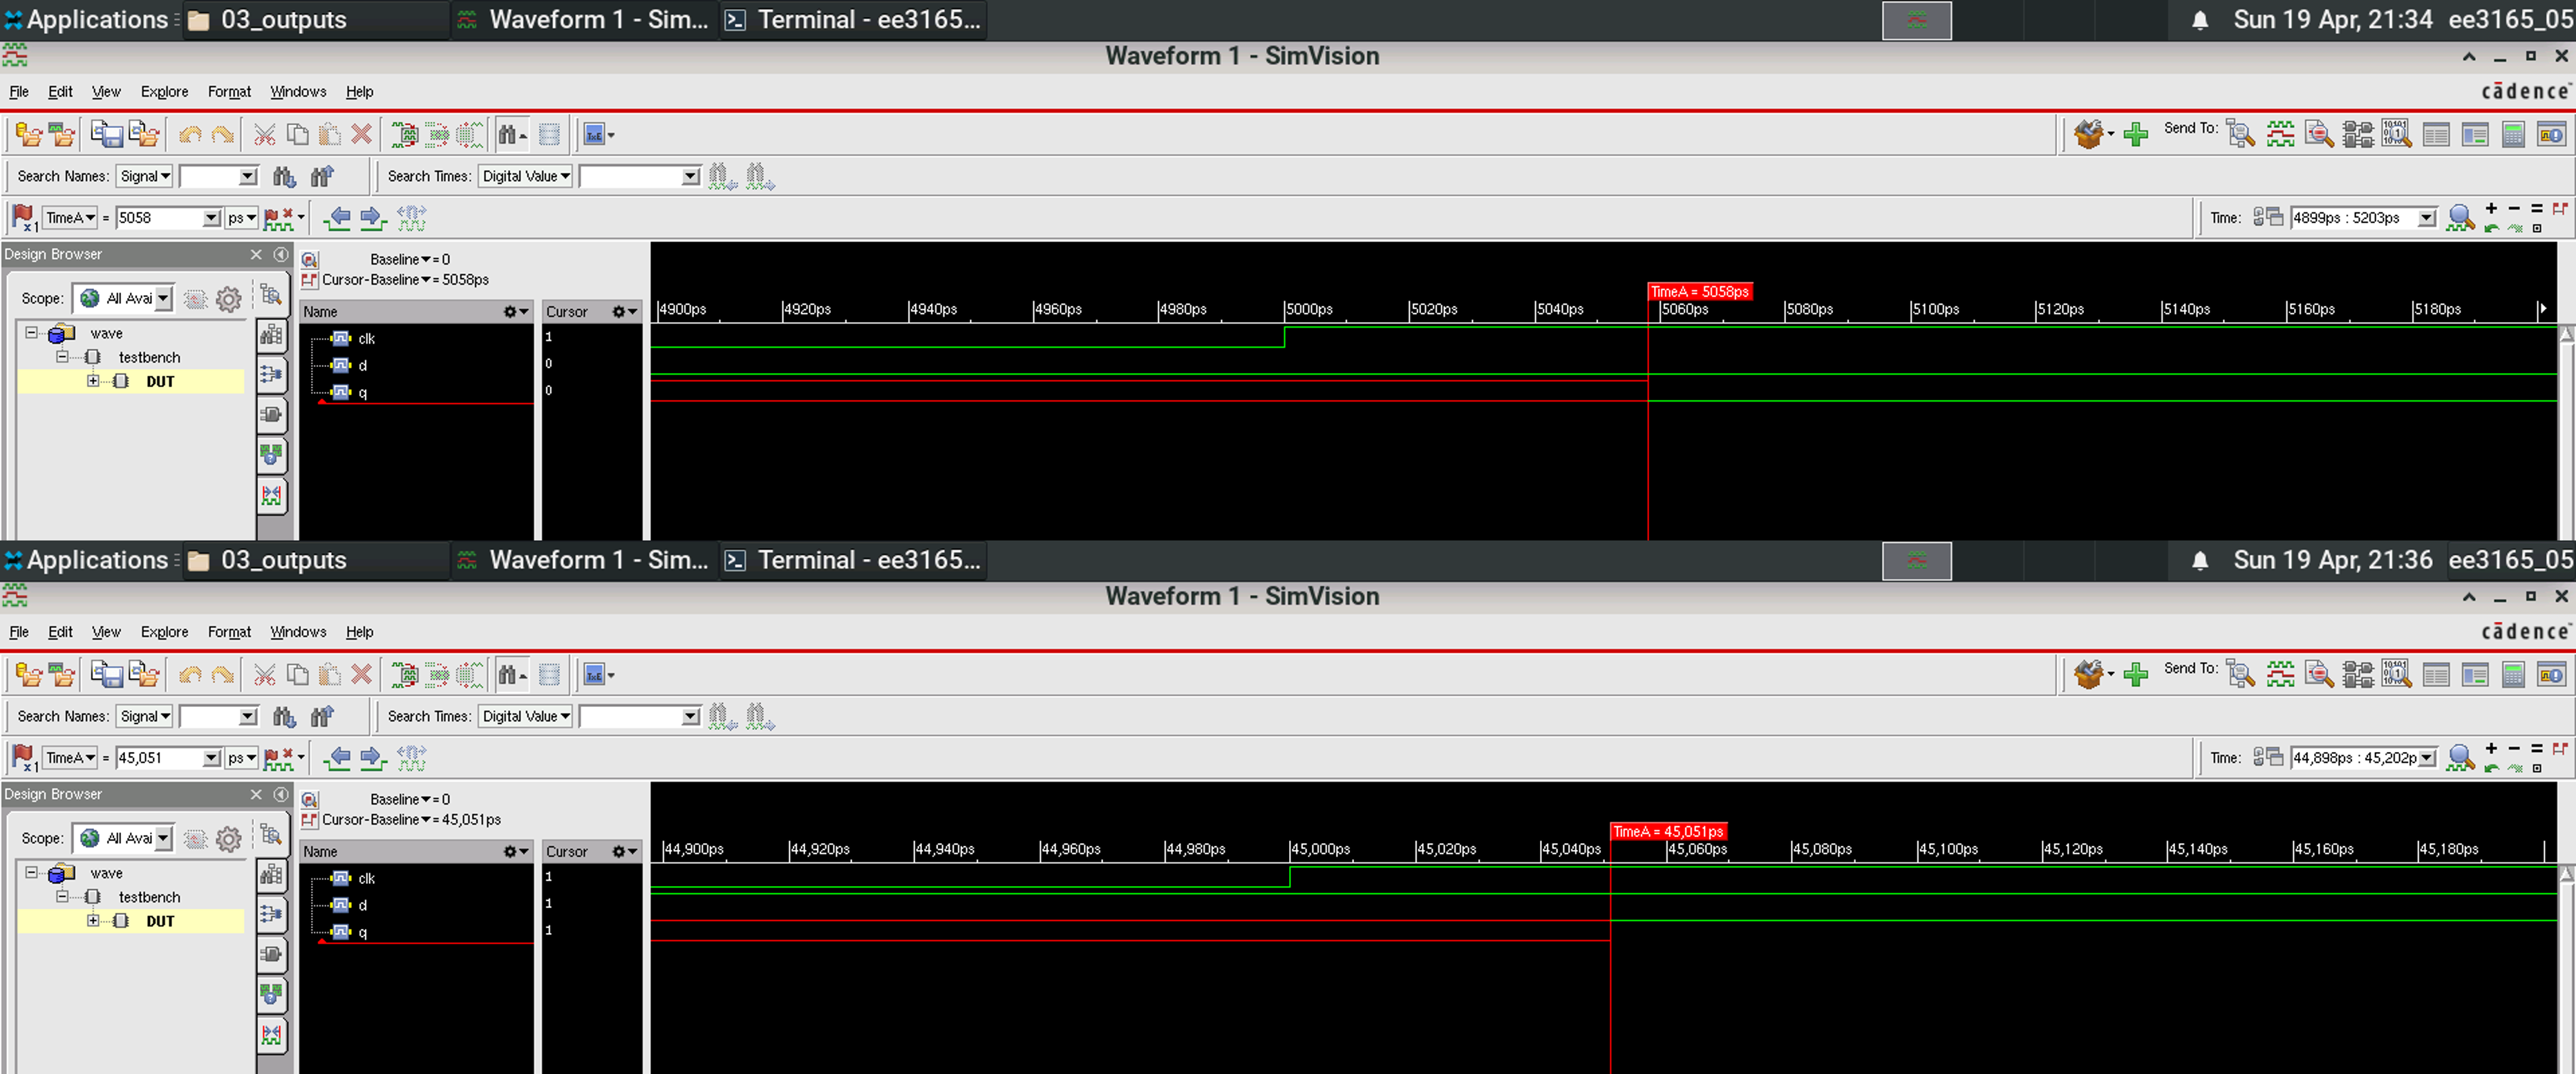
\includegraphics[width=\textwidth]{figures/dff_hvt_fast1v0_delay.png}
        \caption{Corner HVT Fast (fast\_vdd1v0)}
    \end{subfigure}
    \hfill 
    \begin{subfigure}[b]{0.48\textwidth}
        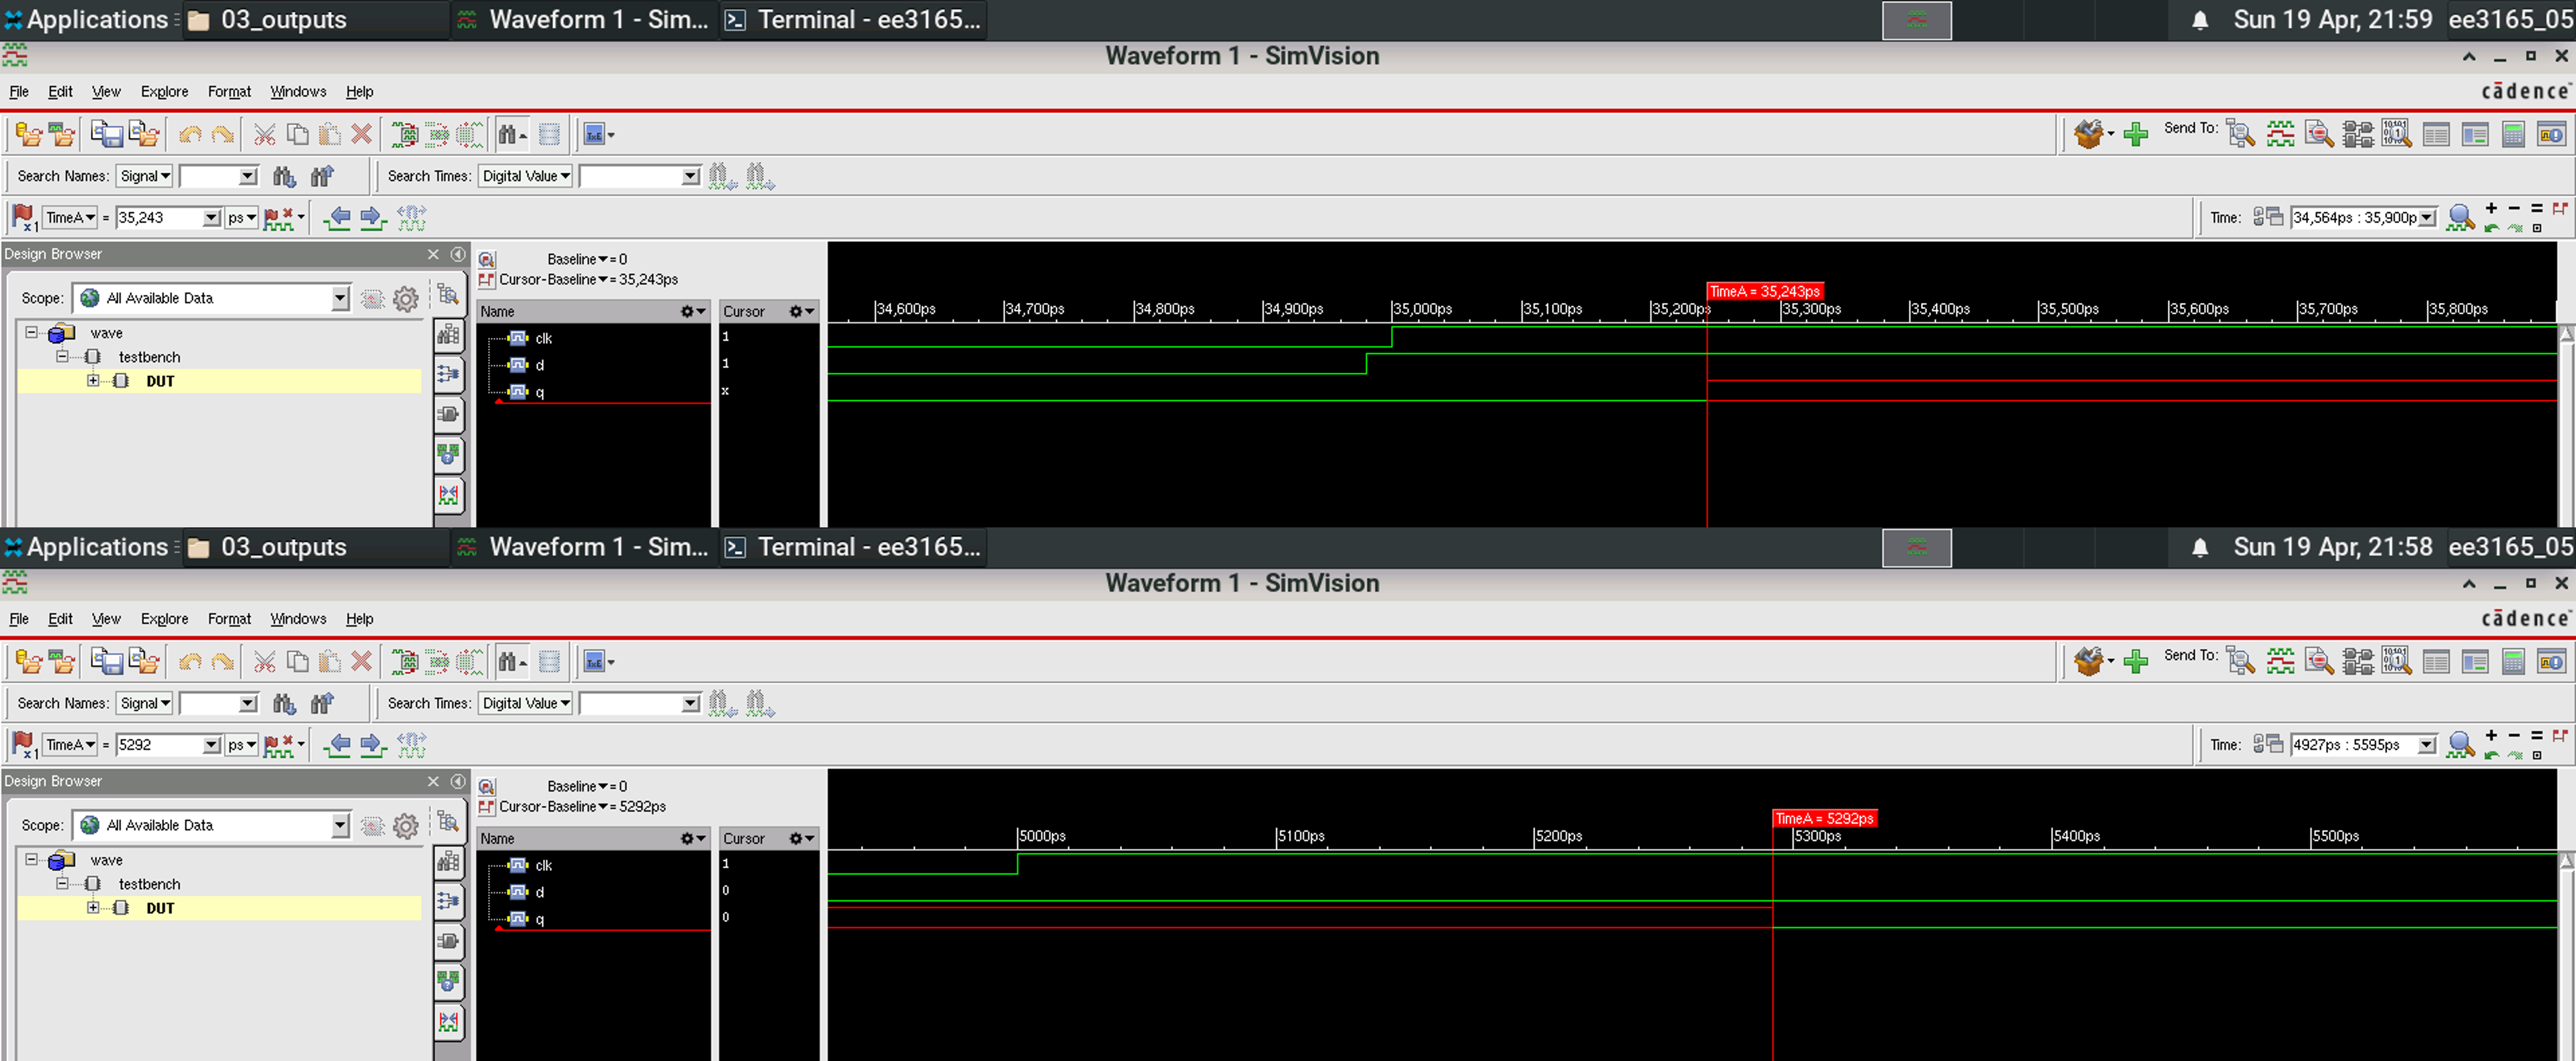
\includegraphics[width=\textwidth]{figures/dff_hvt_slow1v0_delay.png}
        \caption{Corner HVT Slow (slow\_vdd1v0)}
    \end{subfigure}
    \caption{Waveform đo độ trễ D-FF ở High Threshold Voltage (VDD = 1.0\,V).
    Hình trên: waveform khi D chuyển lên mức 1 (Rising Delay).
    Hình dưới: waveform khi D chuyển xuống mức 0 (Falling Delay).}
    \label{fig:dff_hvt_1v0_delay}
\end{figure}

\textbf{Nhận xét (HVT -- 1.0\,V):}
\begin{itemize}
    \item \textbf{Hiện tượng đói dòng:} Do điện áp ngưỡng ($V_{th}$) của cell HVT cao,
    khi hạ $V_{DD}$ xuống 1.0\,V, điện áp quá lái $V_{OV} = V_{DD} - V_{th}$ bị thu hẹp
    đáng kể. Dòng bão hòa $I_{on}$ suy giảm, làm chậm quá trình nạp/xả tụ ký sinh tại
    ngõ ra Q.
    \item \textbf{Độ trễ cao nhất ở góc Slow:} Tại corner \texttt{slow\_vdd1v0\_hvt},
    $t_{pHL}$ đạt 0.292\,ns -- mức worst-case lớn nhất trong 8 corners. Đây là ràng buộc
    quyết định tần số hoạt động tối đa của mạch tuần tự (tần số $f_{max} \leq 1/(t_{CK\to Q}
    + t_{setup} + t_{routing})$).
    \item \textbf{Tối ưu năng lượng:} Bù lại, tổng công suất tại góc này đạt mức thấp nhất
    ($4.932\times10^{-8}$\,W), phù hợp với các ứng dụng không yêu cầu tần số cao.
\end{itemize}

\paragraph{2. Khảo sát HVT tại điện áp danh định (VDD = 1.2\,V)}

\begin{figure}[H]
    \centering
    \begin{subfigure}[b]{0.48\textwidth}
        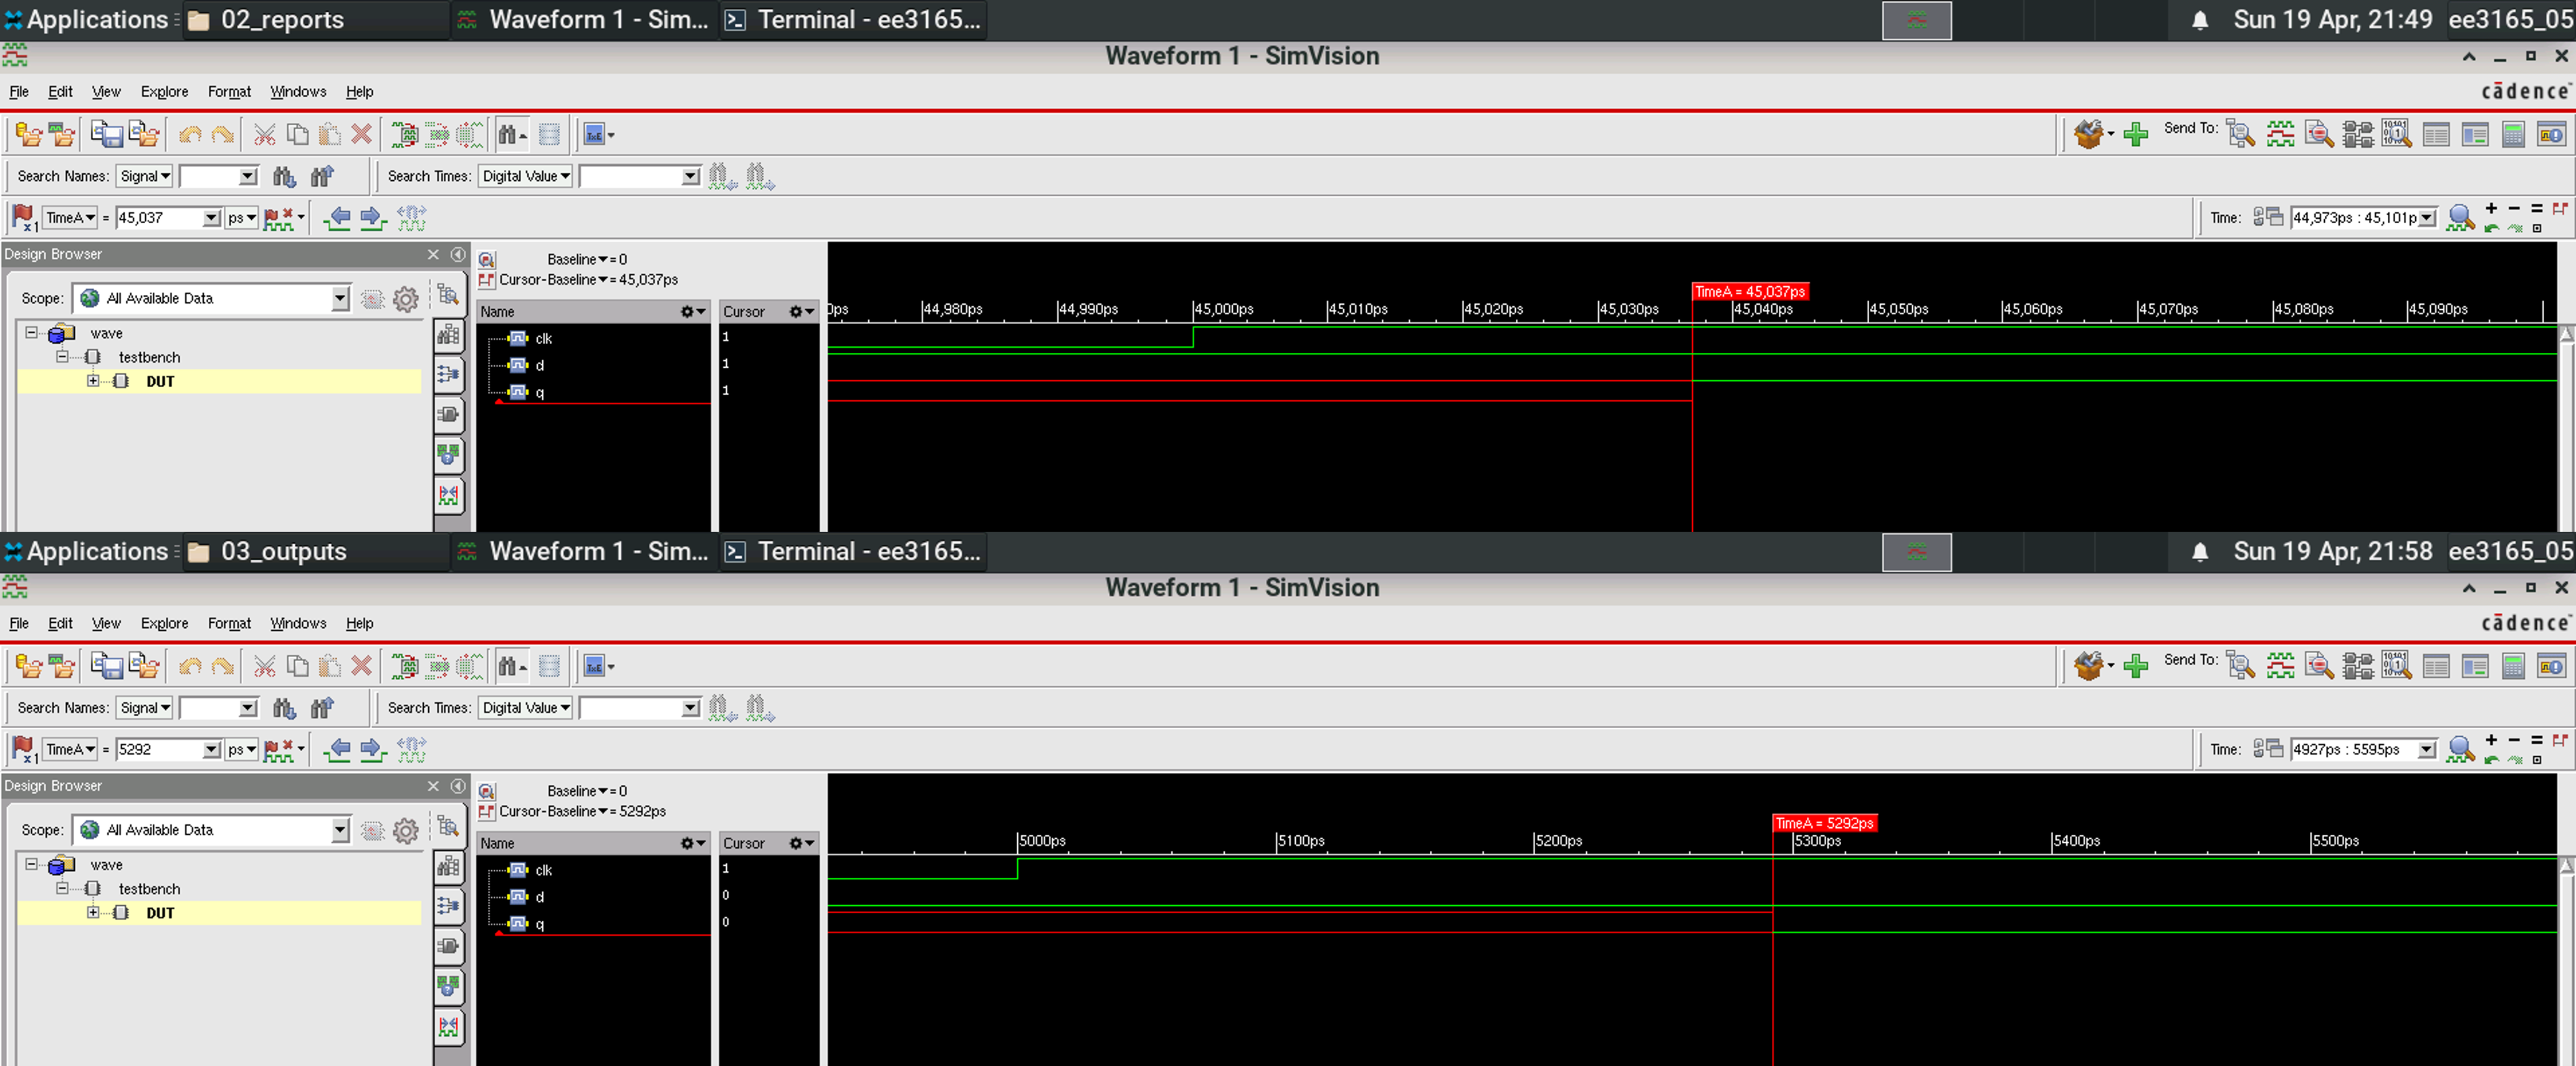
\includegraphics[width=\textwidth]{figures/dff_hvt_fast1v2_delay.png}
        \caption{Corner HVT Fast (fast\_vdd1v2)}
    \end{subfigure}
    \hfill
    \begin{subfigure}[b]{0.48\textwidth}
        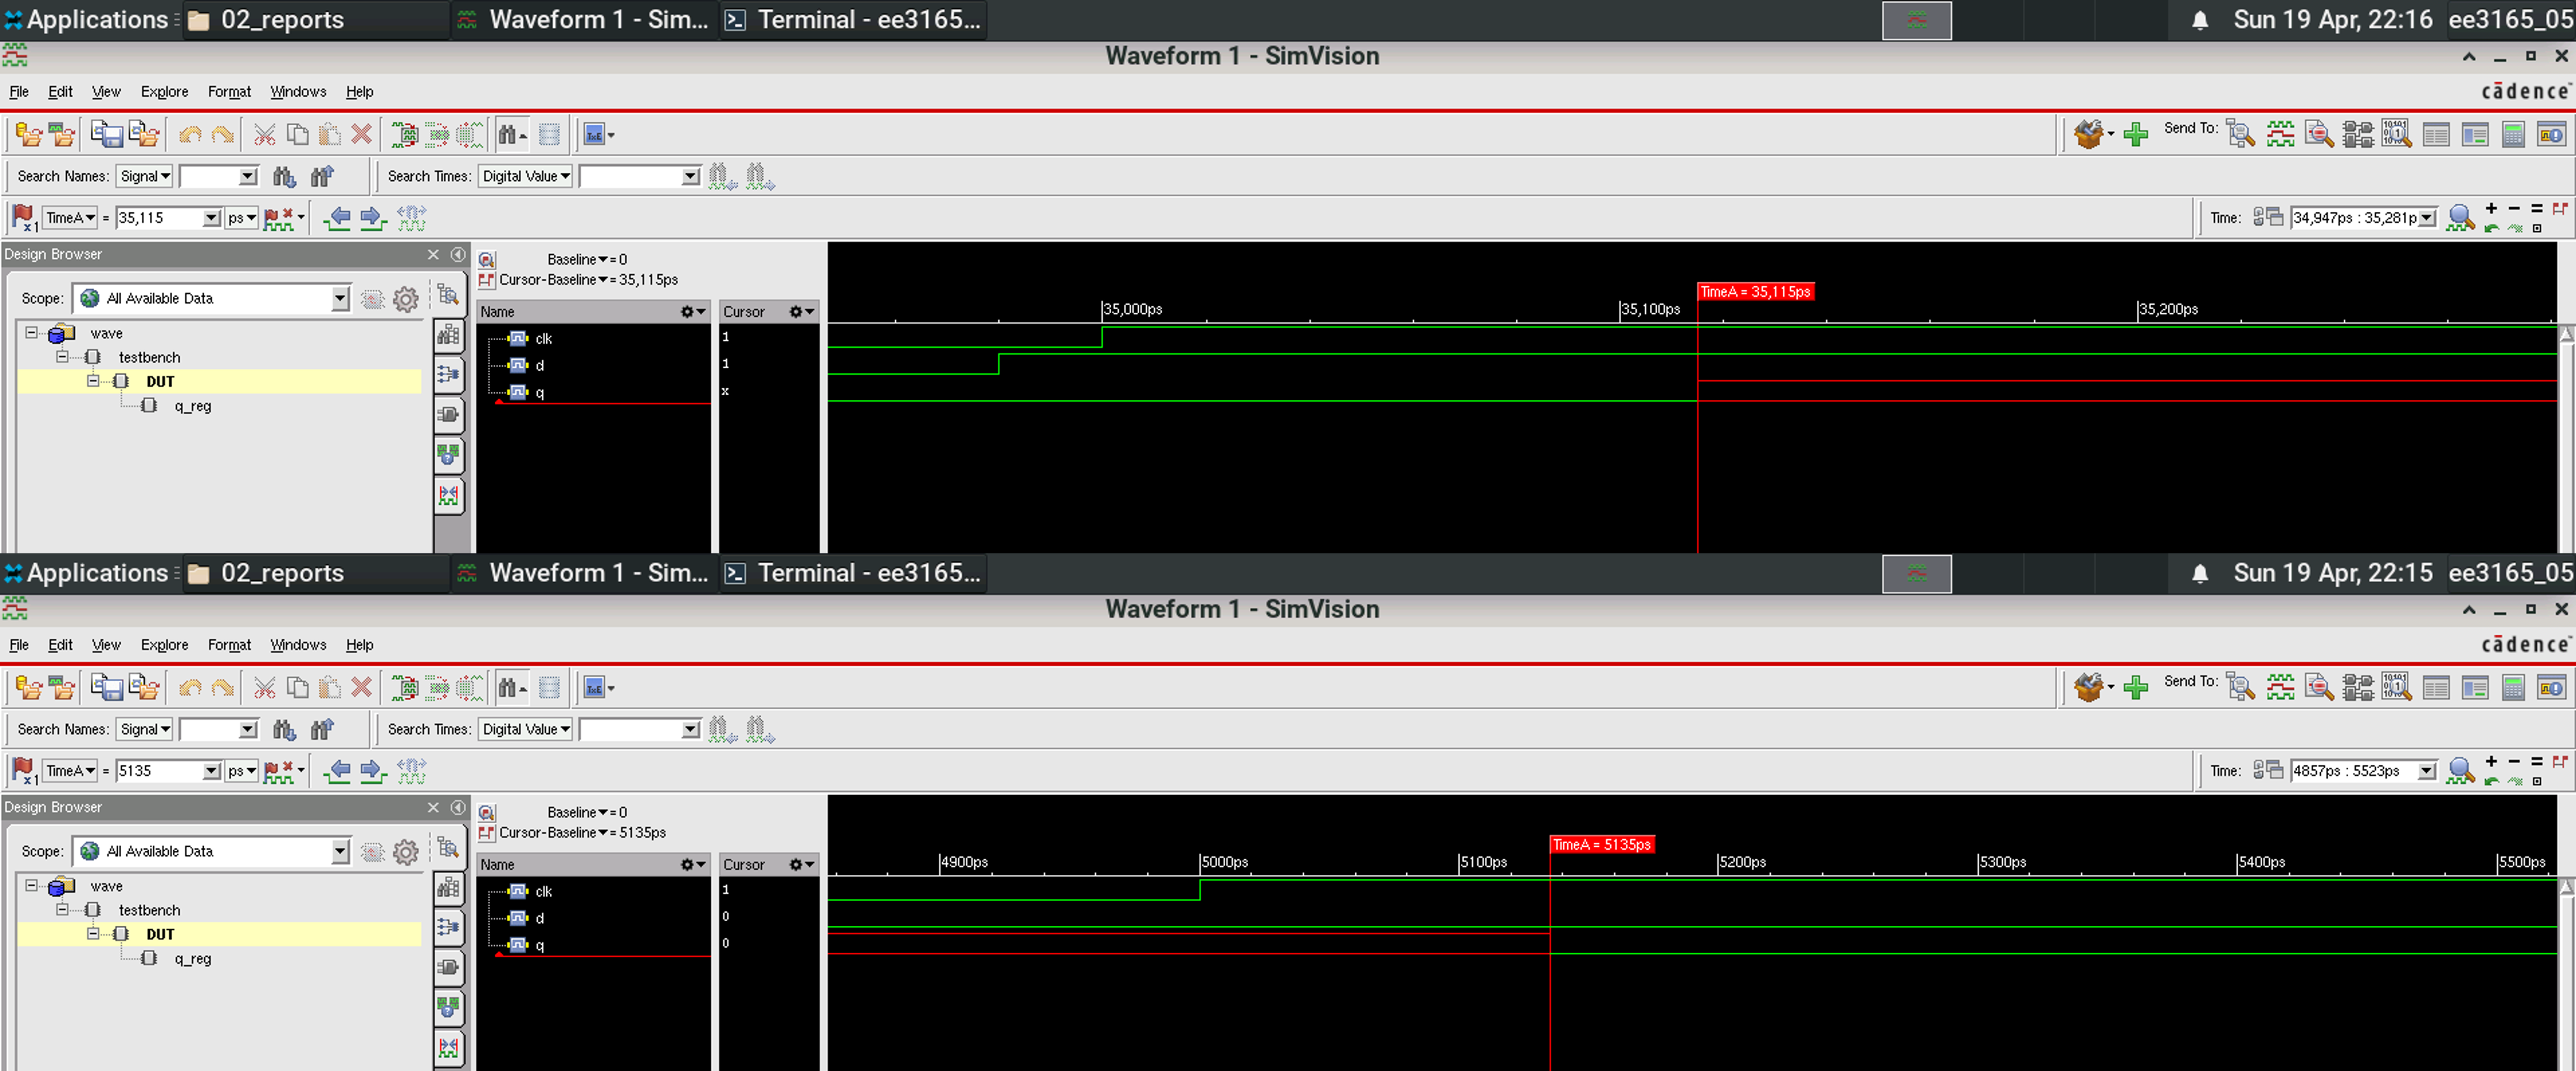
\includegraphics[width=\textwidth]{figures/dff_hvt_slow1v2_delay.png}
        \caption{Corner HVT Slow (slow\_vdd1v2)}
    \end{subfigure}
    \caption{Waveform đo độ trễ D-FF ở High Threshold Voltage (VDD = 1.2\,V).}
    \label{fig:dff_hvt_1v2_delay}
\end{figure}

\textbf{Nhận xét (HVT -- 1.2\,V):}
\begin{itemize}
    \item \textbf{Cải thiện tốc độ rõ rệt:} Nâng $V_{DD}$ lên 1.2\,V giúp tăng $V_{OV}$,
    qua đó tăng $I_{on}$. So với mức 1.0\,V, $t_{pHL}$ tại góc \texttt{fast\_vdd1v2\_hvt}
    giảm từ 0.058\,ns xuống 0.042\,ns -- cải thiện khoảng 28\%.
    \item \textbf{Sự đánh đổi về công suất:} Công suất tổng tăng do thành phần công suất
    động tỉ lệ với $V_{DD}^2$ ($P_{dyn} \propto C \cdot V_{DD}^2 \cdot f$).
    \item \textbf{Góc phù hợp cho thiết kế cân bằng:} Thư viện HVT tại 1.2\,V là lựa chọn
    lý tưởng cho phần lớn các thanh ghi trong thiết kế, đảm bảo cả hiệu năng lẫn khả năng
    kiểm soát rò rỉ điện tốt.
\end{itemize}

% -------------------------------------------------------
\subsubsection*{B. Thư viện Low Threshold Voltage (LVT)}

Các cell LVT cho tốc độ chuyển mạch nhanh hơn nhờ điện áp ngưỡng thấp, đổi lại công
suất tiêu thụ tĩnh sẽ cao hơn đáng kể.

\paragraph{1. Khảo sát LVT tại điện áp thấp (VDD = 1.0\,V)}

\begin{figure}[H]
    \centering
    \begin{subfigure}[b]{0.48\textwidth}
        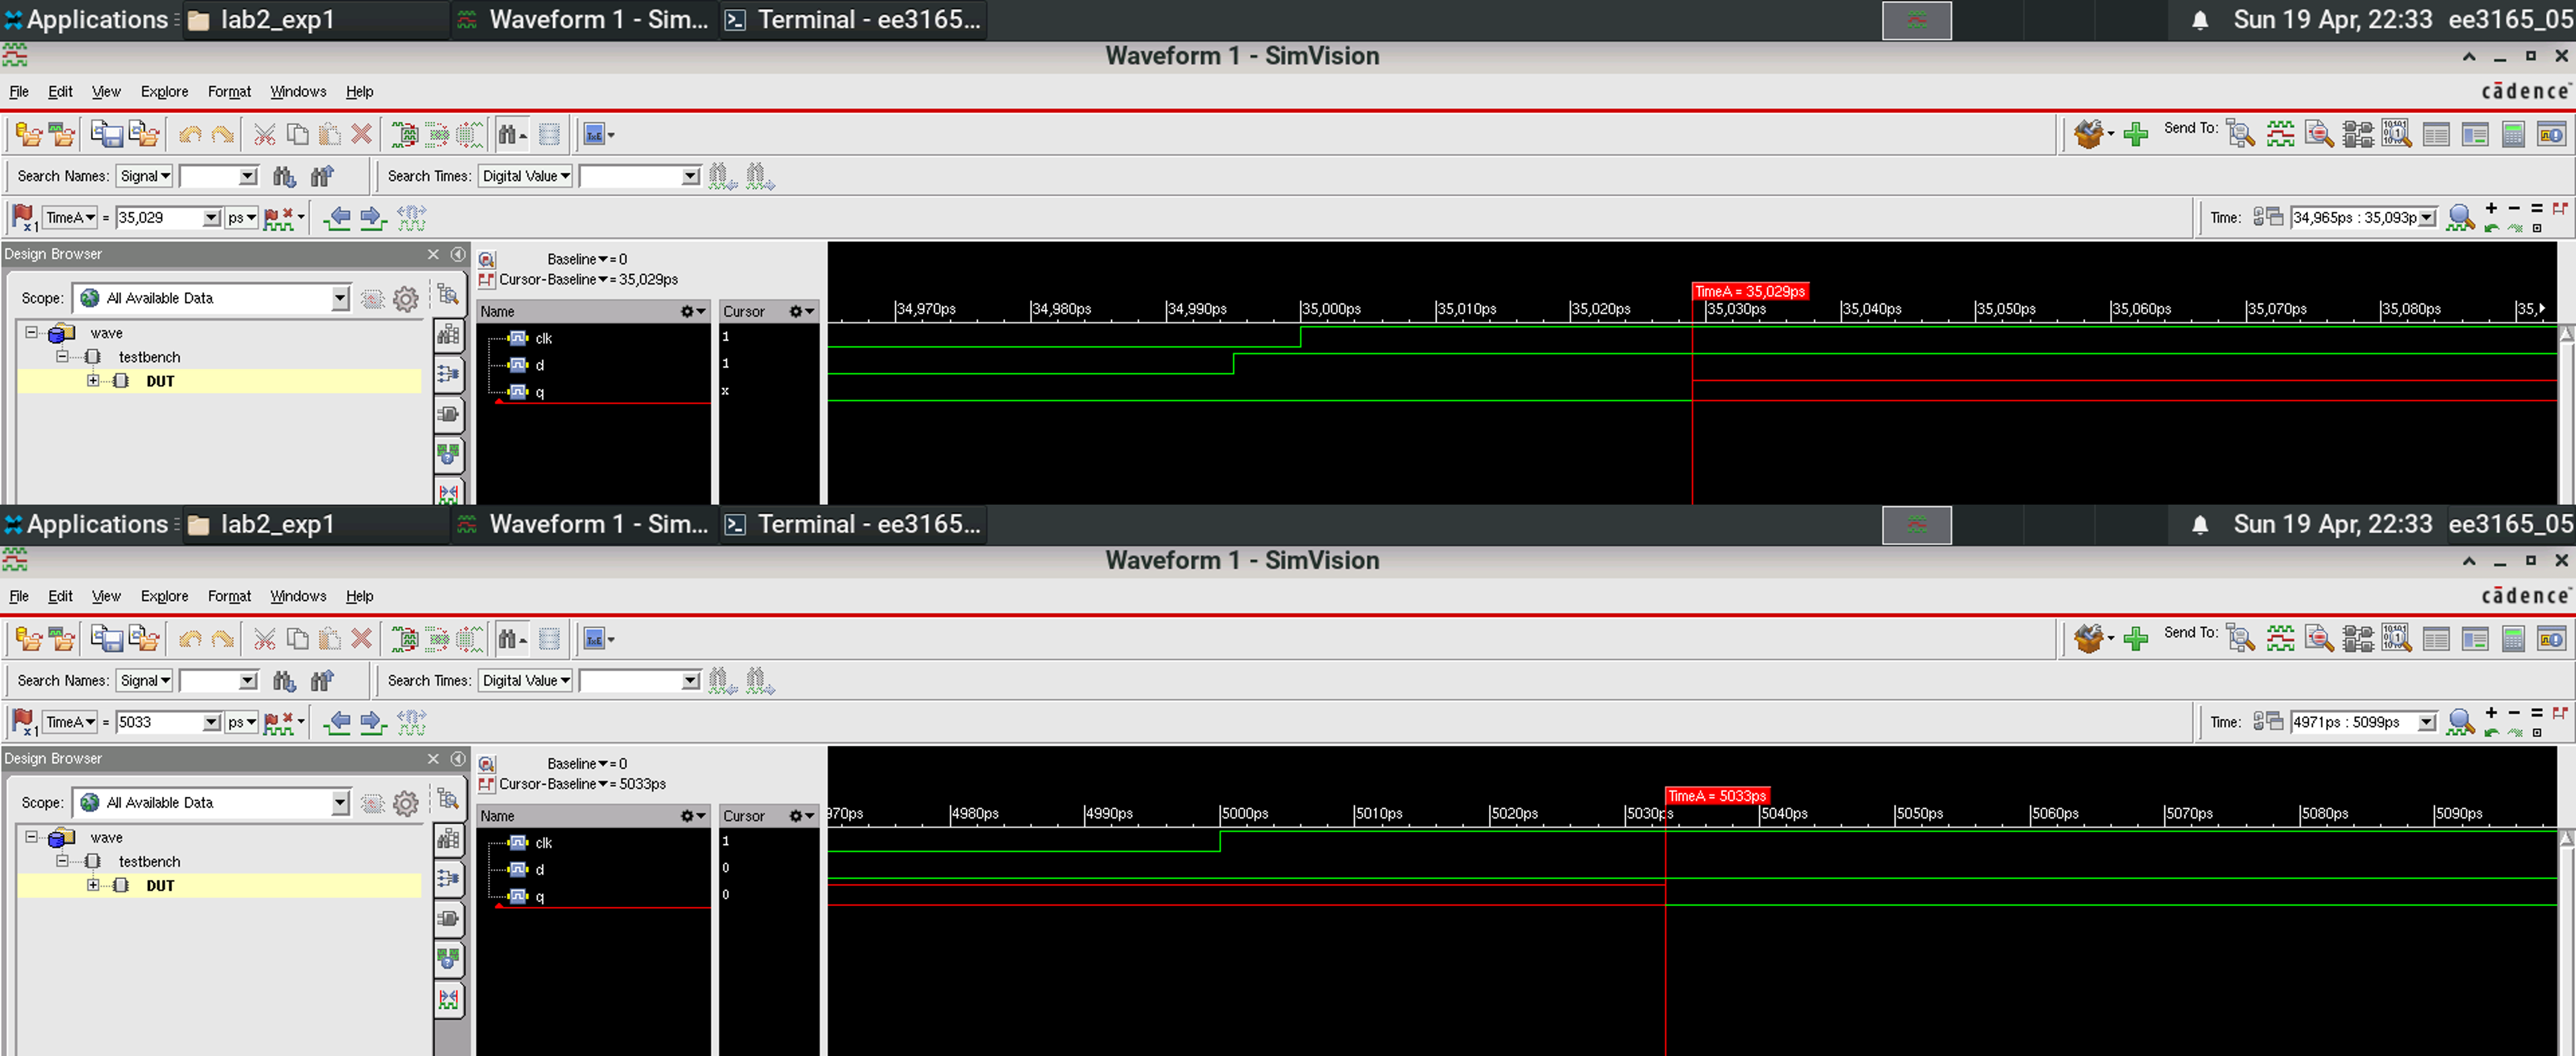
\includegraphics[width=\textwidth]{figures/dff_lvt_fast1v0_delay.png}
        \caption{Corner LVT Fast (fast\_vdd1v0)}
    \end{subfigure}
    \hfill
    \begin{subfigure}[b]{0.48\textwidth}
        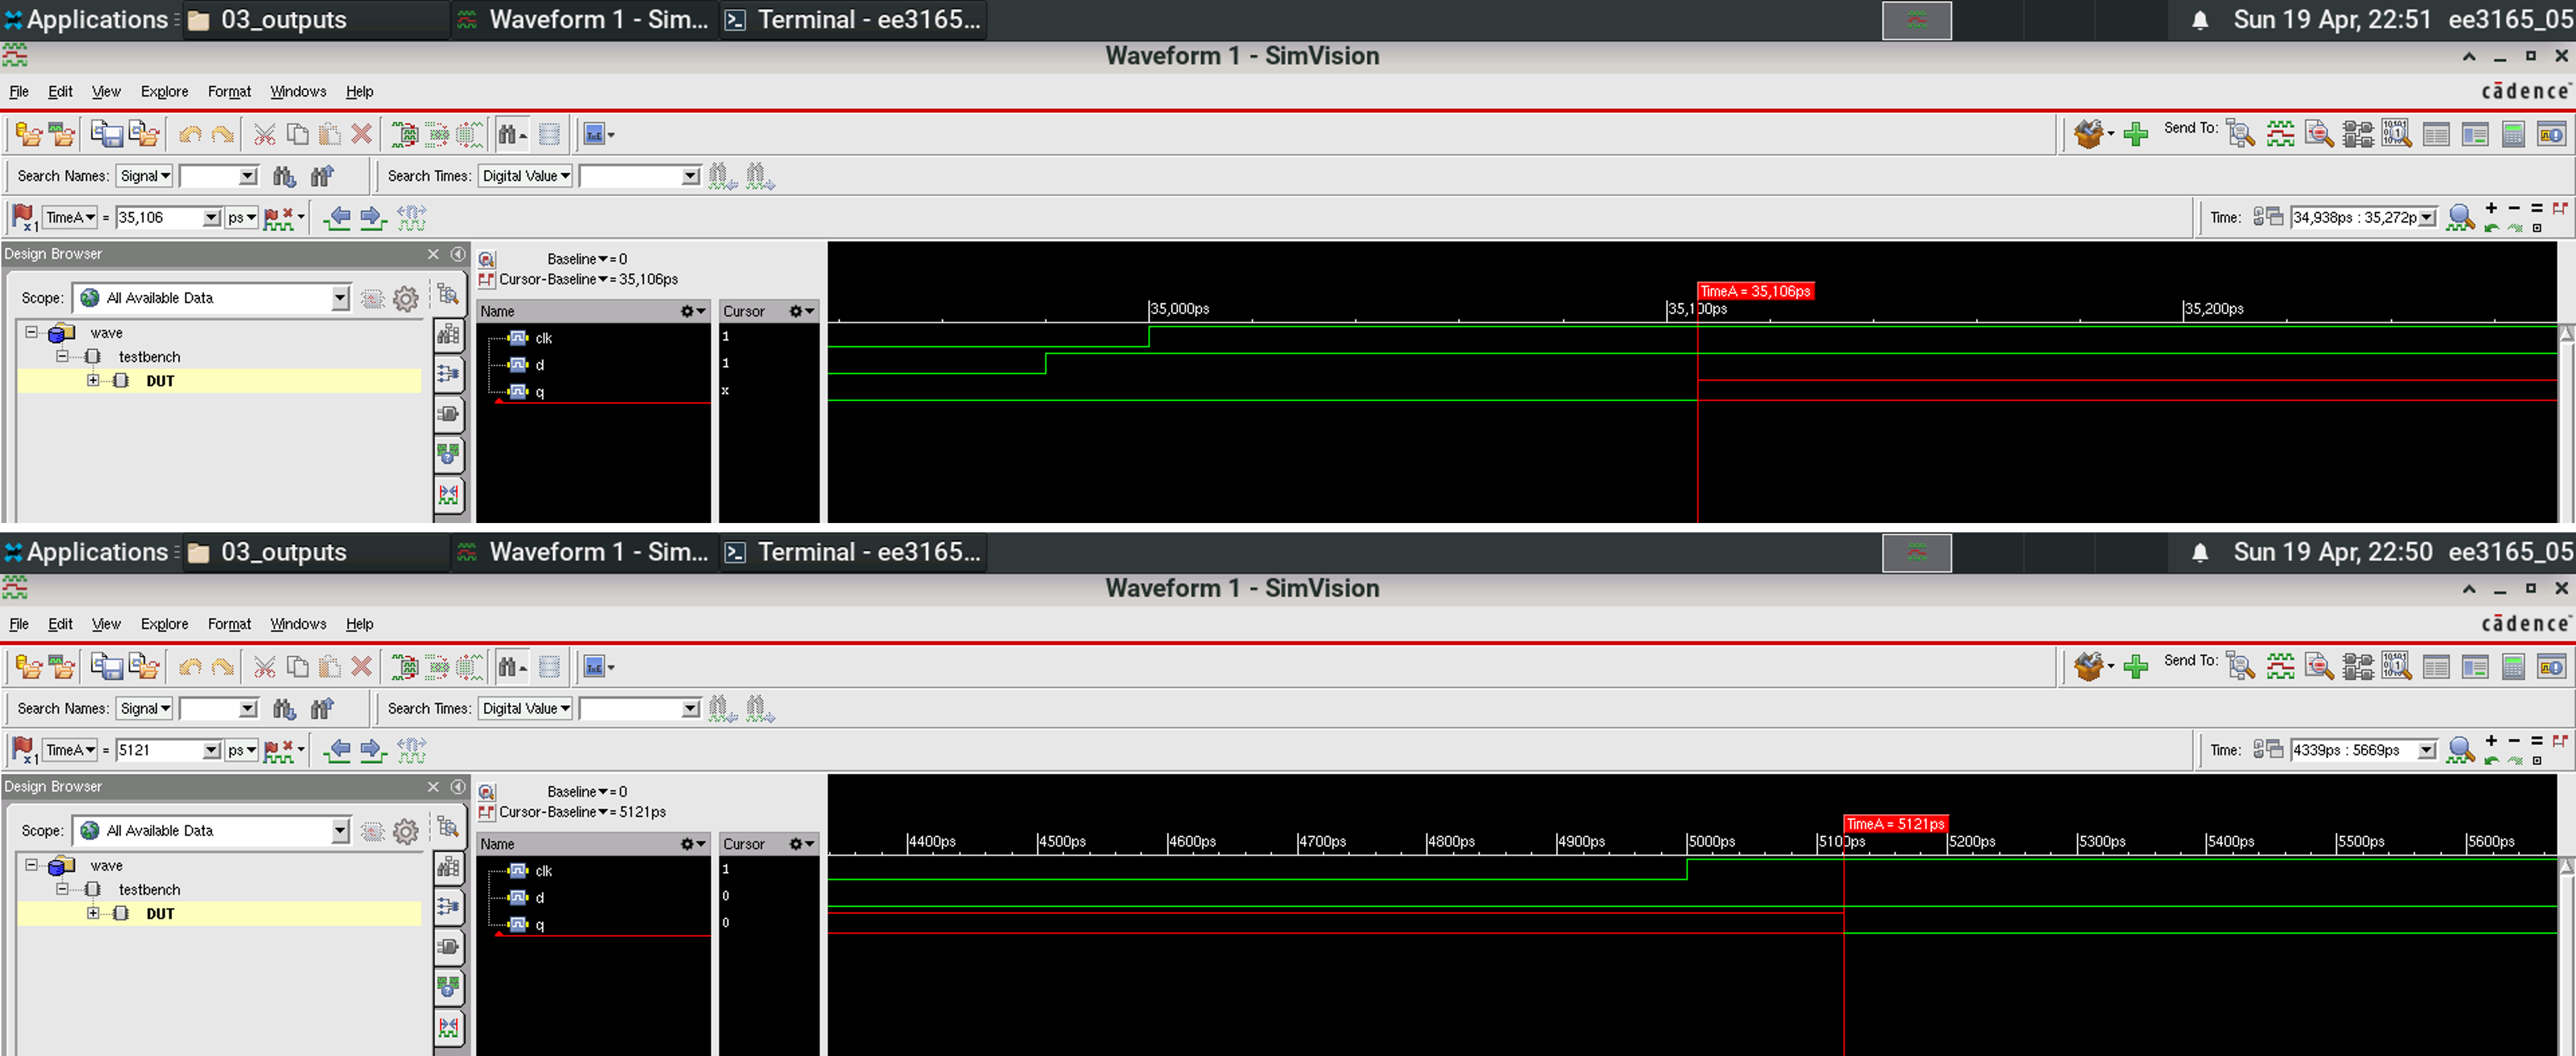
\includegraphics[width=\textwidth]{figures/dff_lvt_slow1v0_delay.png}
        \caption{Corner LVT Slow (slow\_vdd1v0)}
    \end{subfigure}
    \caption{Waveform đo độ trễ D-FF sử dụng thư viện LVT tại VDD = 1.0\,V.}
    \label{fig:dff_lvt_1v0_delay}
\end{figure}

\textbf{Nhận xét (LVT -- 1.0\,V):}
\begin{itemize}
    \item \textbf{Khả năng duy trì tốc độ:} Nhờ $V_{th}$ thấp, $V_{OV}$ của các transistor
    LVT vẫn đủ lớn ngay cả khi $V_{DD}$ chỉ còn 1.0\,V. Tại góc \texttt{slow\_vdd1v0\_lvt},
    $t_{pHL}$ chỉ là 0.121\,ns -- nhanh hơn đáng kể so với 0.292\,ns của HVT ở cùng điều kiện
    (cải thiện gần 60\%).
    \item \textbf{Ưu thế trong thiết kế Low Power:} Khi hệ thống bị giới hạn về điện áp nguồn
    (ứng dụng IoT, pin), D-FF LVT tại 1.0\,V giúp đảm bảo mạch tuần tự vẫn đáp ứng được ràng
    buộc Setup Time mà không cần nâng $V_{DD}$.
    \item \textbf{Sự đánh đổi về công suất tĩnh:} Dòng rò rỉ dưới ngưỡng (sub-threshold
    leakage) của LVT vẫn cao hơn HVT ngay cả ở 1.0\,V, do rào cản thế thấp.
\end{itemize}

\paragraph{2. Khảo sát LVT tại điện áp danh định (VDD = 1.2\,V)}

\begin{figure}[H]
    \centering
    \begin{subfigure}[b]{0.48\textwidth}
        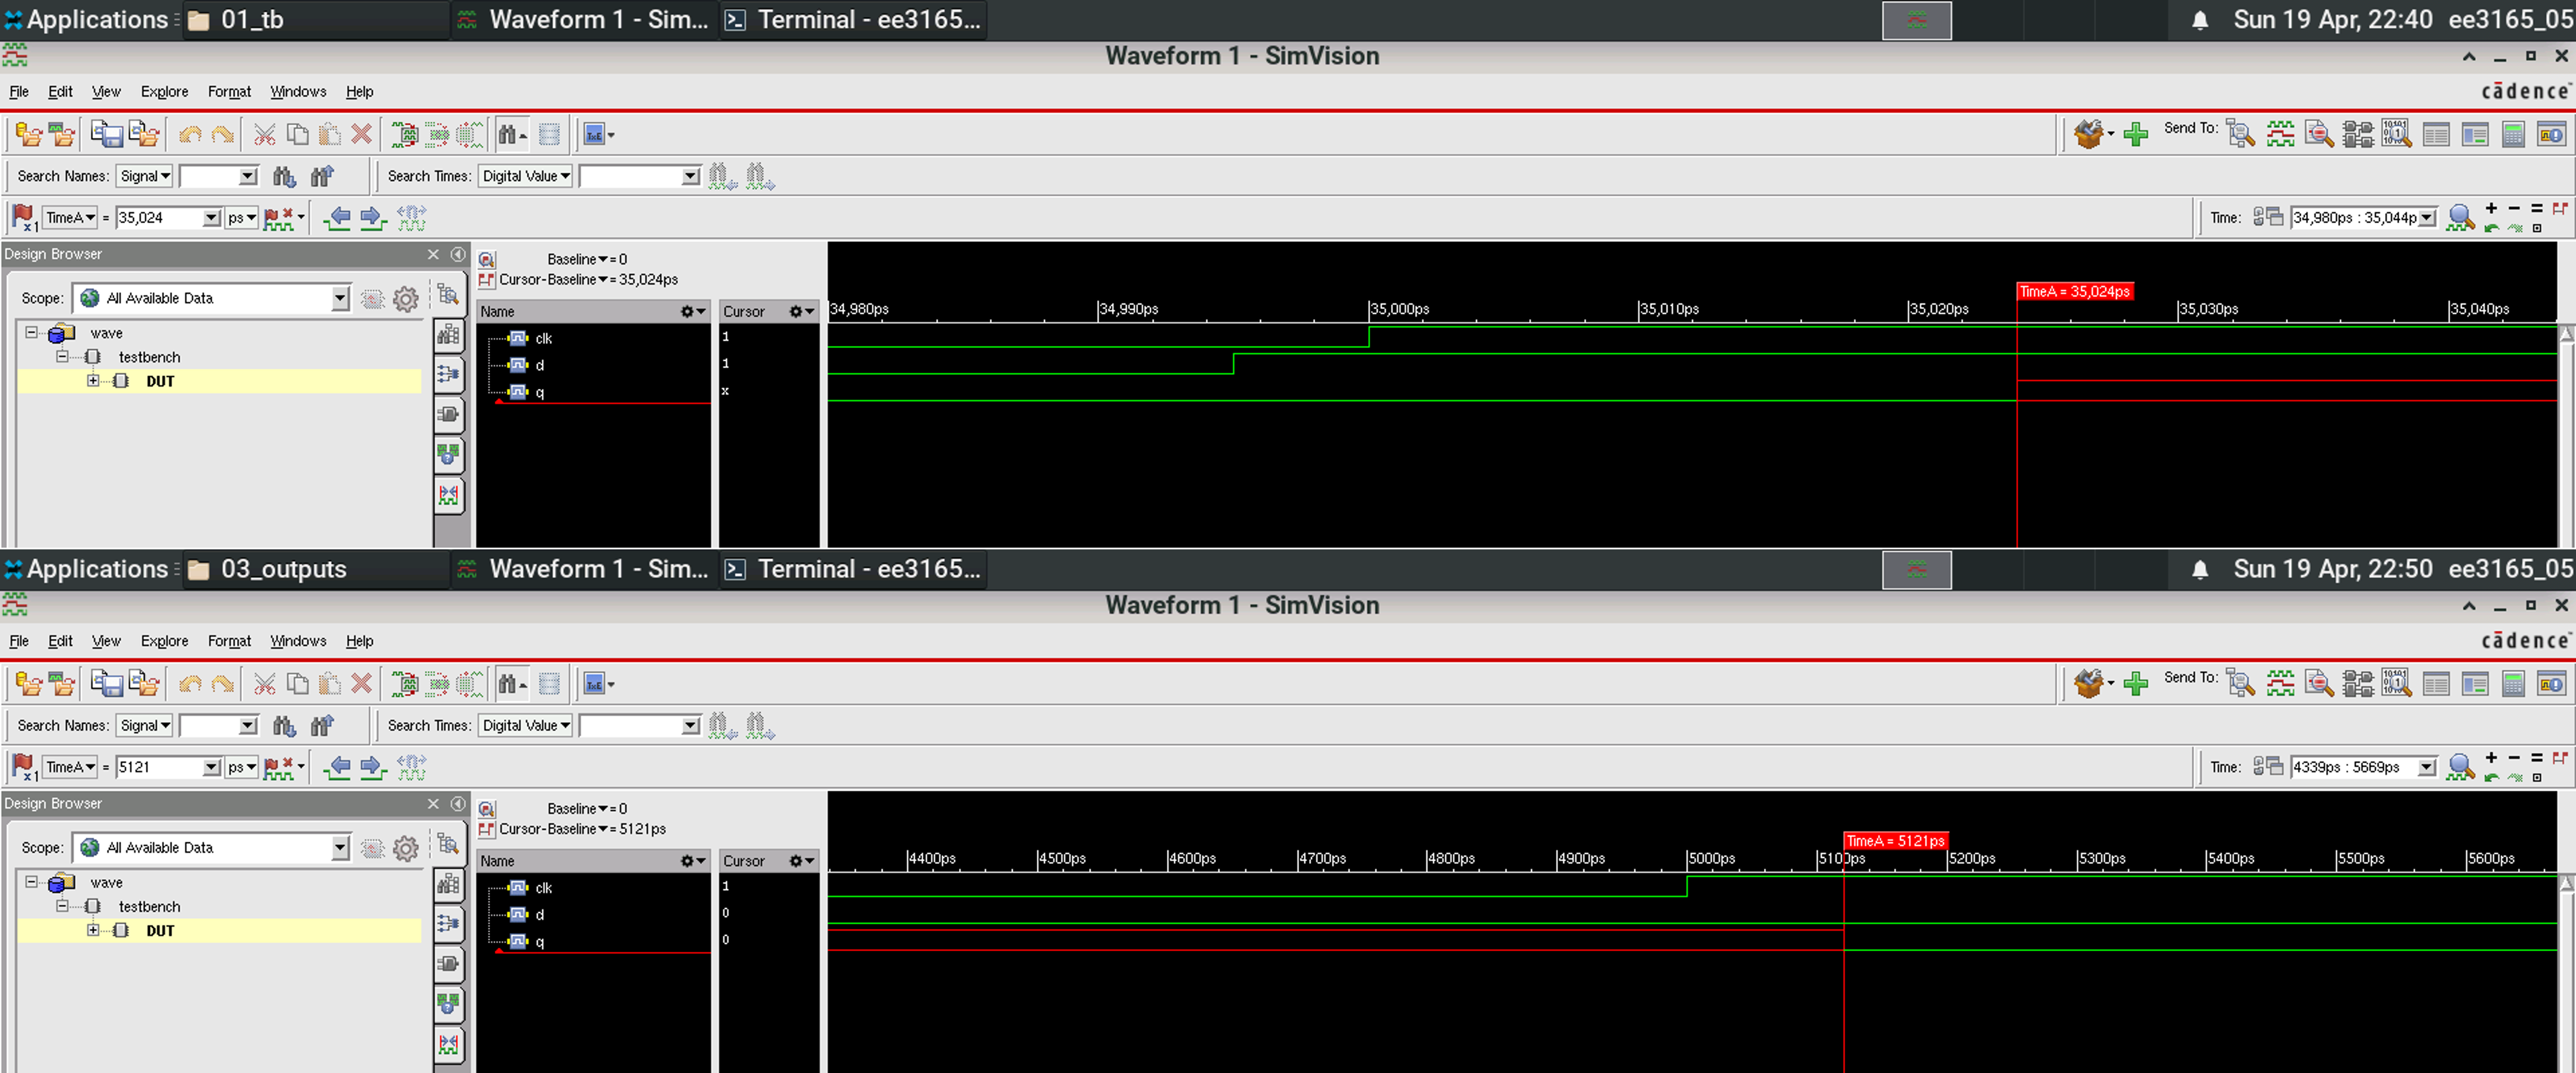
\includegraphics[width=\textwidth]{figures/dff_lvt_fast1v2_delay.png}
        \caption{Corner LVT Fast (fast\_vdd1v2)}
    \end{subfigure}
    \hfill 
    \begin{subfigure}[b]{0.48\textwidth}
        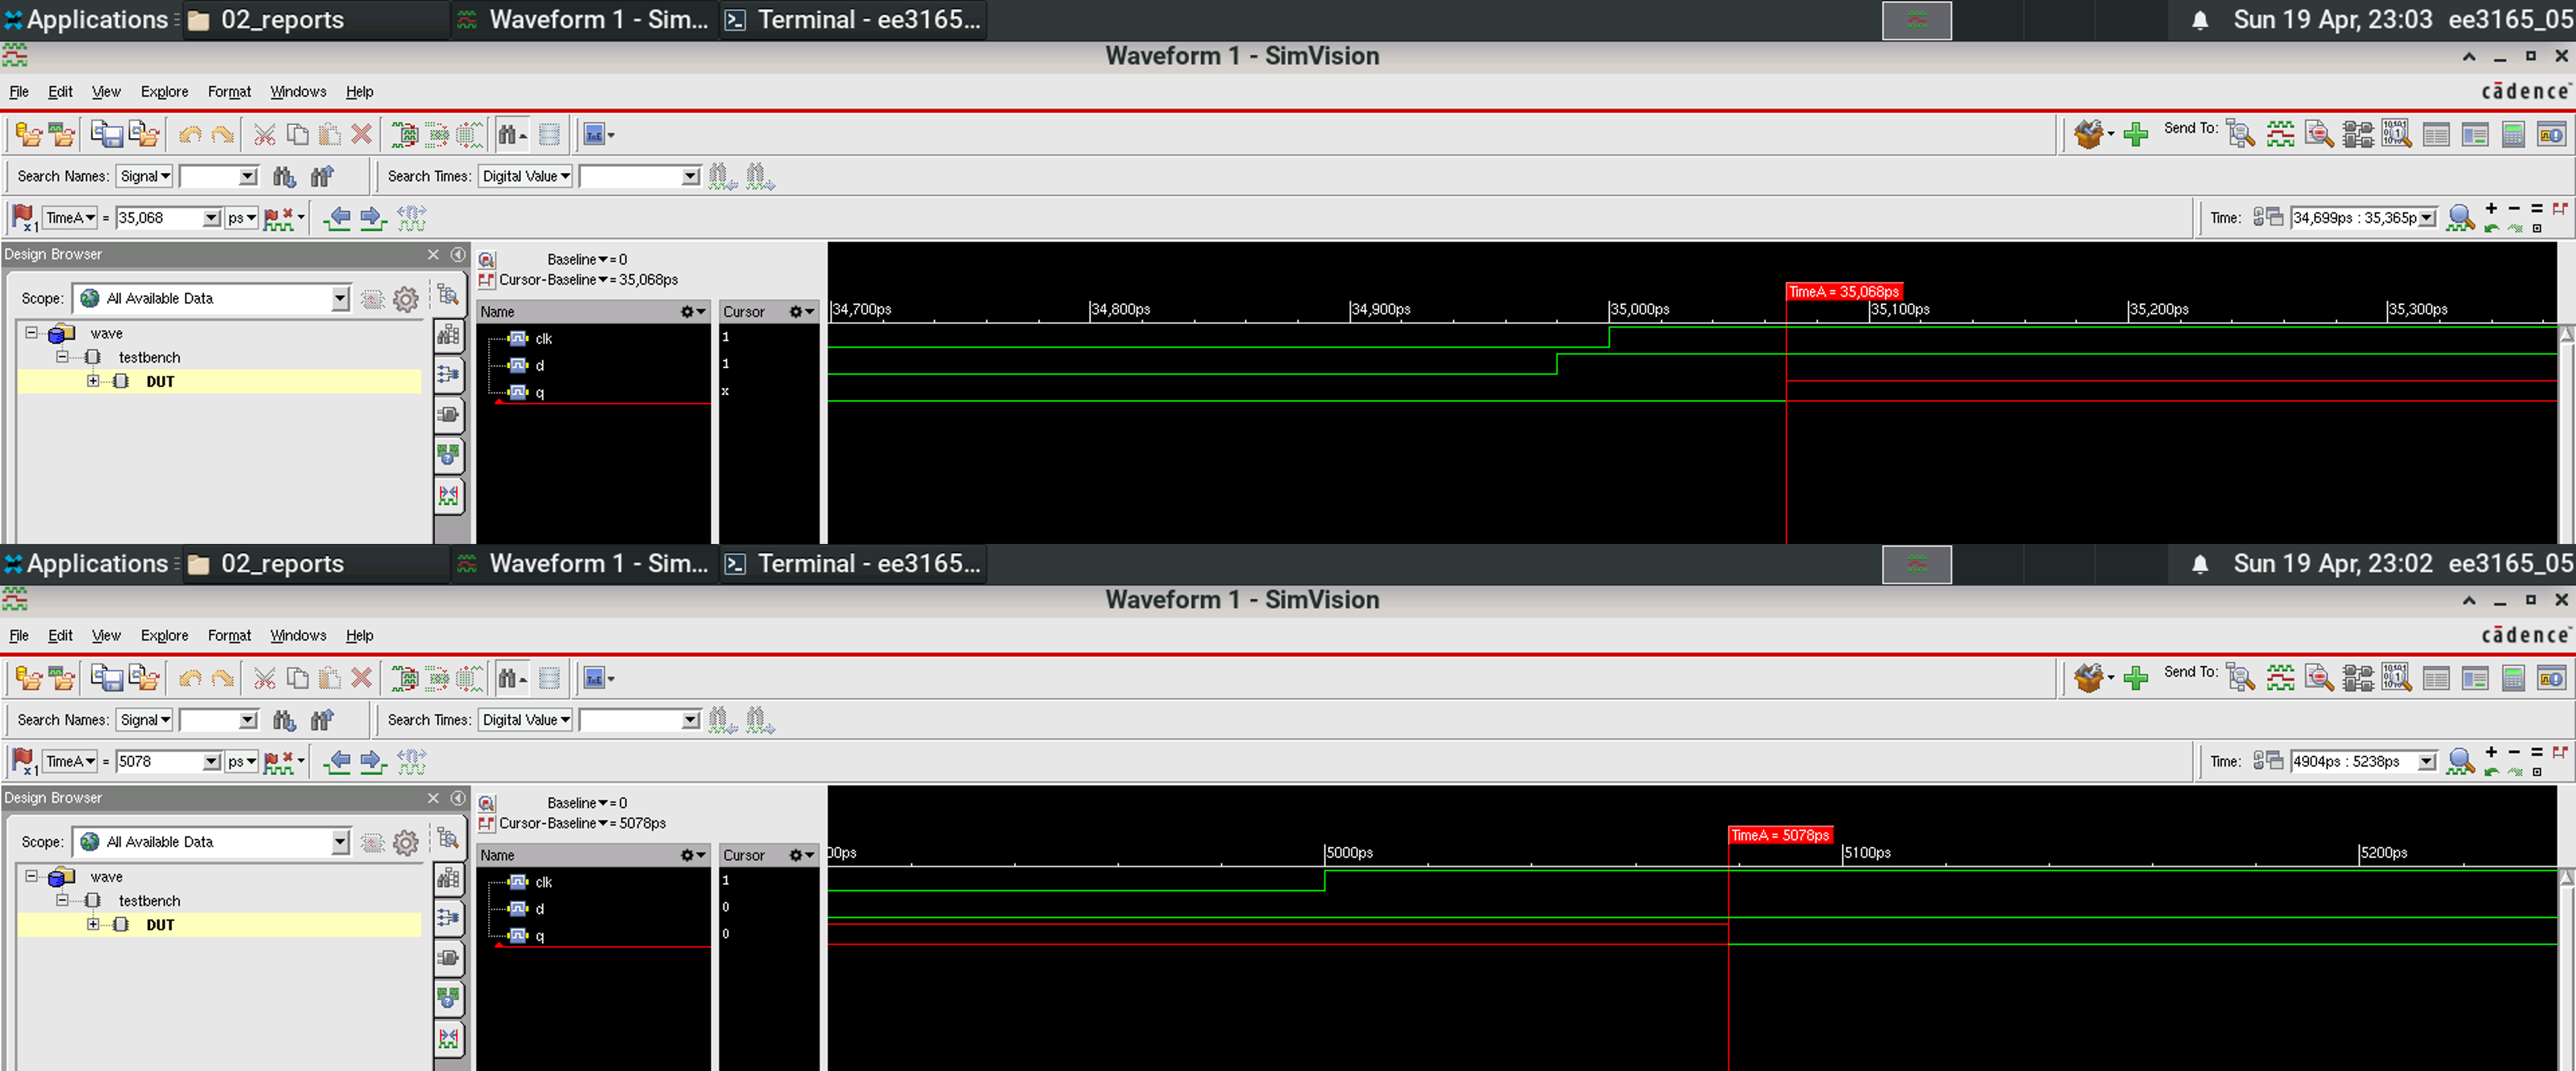
\includegraphics[width=\textwidth]{figures/dff_lvt_slow1v2_delay.png}
        \caption{Corner LVT Slow (slow\_vdd1v2)}
    \end{subfigure}
    \caption{Waveform đo độ trễ D-FF sử dụng thư viện LVT tại VDD = 1.2\,V.}
    \label{fig:dff_lvt_1v2_delay}
\end{figure}

\textbf{Nhận xét (LVT -- 1.2\,V):}
\begin{itemize}
    \item \textbf{Tốc độ cực hạn (Best-case Delay):} Sự kết hợp giữa $V_{th}$ thấp và $V_{DD}$
    cao tạo ra $I_{on}$ cực đại. Tại góc \texttt{fast\_vdd1v2\_lvt}, $t_{pLH}$ đạt 0.024\,ns và
    $t_{pHL}$ đạt 0.027\,ns -- đây là mức độ trễ thấp nhất trong tất cả 8 corners. Cấu hình
    này quyết định $f_{max}$ của toàn bộ chip.
    \item \textbf{Gia tăng công suất tĩnh:} Đây cũng là điều kiện mà dòng rò rỉ đạt mức cực
    đại ($1.047\times10^{-7}$\,W). Trong thực tế, kỹ sư chỉ nên dùng LVT tại 1.2\,V cho các
    thanh ghi nằm trên đường dẫn tới hạn (critical path), tránh lạm dụng gây ra vấn đề về
    nhiệt (thermal issues).
\end{itemize}

% -------------------------------------------------------
\subsubsection*{C. Kết luận}

Phân tích tổng thể D-FF qua 8 process corners cho thấy các quy luật tương tự với các
cổng logic tổ hợp đã khảo sát ở Experiment~1, nhưng với một số điểm đặc trưng riêng
của phần tử tuần tự:

\begin{itemize}
    \item \textbf{Đối với thư viện (HVT vs.\ LVT):} Thư viện LVT mang lại
    tốc độ chuyển mạch vượt trội nhưng dòng rò rỉ lớn. Trong thực tế, công cụ tổng hợp
    sẽ ưu tiên dùng D-FF HVT cho phần lớn thanh ghi và chỉ chèn D-FF LVT vào các thanh
    ghi nằm trên critical path.
    \item \textbf{Đối với giá trị điện áp (1.2\,V vs.\ 1.0\,V):} Hạ áp giúp tiết kiệm
    điện động đáng kể ($P_{dyn} \propto V_{DD}^2$) nhưng kéo dài $t_{CK \to Q}$, làm giảm
    $f_{max}$ của mạch.
    \item \textbf{Đặc trưng của phần tử tuần tự:} Không giống cổng tổ hợp, D-FF còn chịu
    ràng buộc về Setup Time và Hold Time -- các thông số này cũng thay đổi đáng kể theo
    corner PVT và phải được kiểm chứng kỹ lưỡng (xem Mục~2.5).
\end{itemize}

%--------------------------------------------------
\subsection{Setup and Hold time verification}

Dựa trên thông tin được trích xuất từ file SDF sau quá trình tổng hợp, các thông số
ràng buộc thời gian của D-FF được ghi nhận và kiểm chứng qua mô phỏng Gate-level.

Dưới đây là ví dụ nội dung file SDF được trích xuất ở corner \texttt{slow\_vdd1v2\_basicCells\_lvt},
tương ứng với cell \texttt{DFFHQX1LVT}:

\begin{lstlisting}[style={prettyverilog}, caption={SDF}]
(TIMESCALE 1ns)
(CELL
  (CELLTYPE "DFFHQX1LVT")
  (INSTANCE q_reg)
  (DELAY
    (ABSOLUTE
      (PORT CK (::0.000))
      (PORT D  (::0.000))
      (IOPATH CK Q (::0.068) (::0.078))
    )
  )
  (TIMINGCHECK
    (HOLD  (negedge D) (posedge CK) (::0.005))
    (HOLD  (posedge D) (posedge CK) (::0.000))
    (SETUP (negedge D) (posedge CK) (::0.016))
    (SETUP (posedge D) (posedge CK) (::0.036))
  )
)
\end{lstlisting}

Ý nghĩa các thông số trong file SDF:
\begin{itemize}
    \item \textbf{(IOPATH CK Q (::0.068) (::0.078)):} Khi có cạnh lên của xung nhịp CK, ngõ
    ra Q thay đổi sau một khoảng trễ nhất định. Giá trị 0.068\,ns là độ trễ từ cạnh lên CK
    đến khi Q chuyển lên mức 1 ($t_{pLH}$); 0.078\,ns là độ trễ đến khi Q chuyển xuống mức
    0 ($t_{pHL}$).
    \item \textbf{(HOLD (negedge D) (posedge CK) (::0.005)):} Sau cạnh lên của CK, tín hiệu
    D phải giữ ổn định ít nhất 0.005\,ns nếu D vừa chuyển xuống mức 0.
    \item \textbf{(HOLD (posedge D) (posedge CK) (::0.000)):} Nếu D vừa chuyển lên mức 1,
    không cần giữ ổn định sau cạnh lên CK (Hold Time = 0\,ns).
    \item \textbf{(SETUP (negedge D) (posedge CK) (::0.016)):} Tín hiệu D phải ổn định ít
    nhất 0.016\,ns \emph{trước} cạnh lên CK nếu D đang ở sườn xuống.
    \item \textbf{(SETUP (posedge D) (posedge CK) (::0.036)):} Tín hiệu D phải ổn định ít
    nhất 0.036\,ns trước cạnh lên CK nếu D đang ở sườn lên.
\end{itemize}

% LƯU Ý: Để cập nhật bảng khi có file SDF mới, mở file SDF, tìm block (TIMINGCHECK)
% và thay thế các giá trị tương ứng trong bảng bên dưới.
% Cú pháp: (SETUP (posedge D)(posedge CK)(::X)) -> cột "posedge D", hàng corner tương ứng
%           (SETUP (negedge D)(posedge CK)(::X)) -> cột "negedge D"
%           (HOLD  (posedge D)(posedge CK)(::X)) -> cột "posedge D" nhóm Hold
%           (HOLD  (negedge D)(posedge CK)(::X)) -> cột "negedge D" nhóm Hold

Bảng~\ref{tab:exp2_setup_hold} tổng hợp các giá trị Setup Time và Hold Time trích xuất
từ file SDF trên toàn bộ 8 corners.

\begin{table}[H]
    \centering
    \begin{tabular}{|l|c|c|c|c|}
        \hline
        \multirow{2}{*}{\textbf{Library Name}}
            & \multicolumn{2}{c|}{\textbf{Setup Time (ns)}}
            & \multicolumn{2}{c|}{\textbf{Hold Time (ns)}} \\
        \cline{2-5}
            & \textbf{posedge D} & \textbf{negedge D}
            & \textbf{posedge D} & \textbf{negedge D} \\
        \hline
        fast\_vdd1v0\_basicCells\_hvt & 0.025 & 0.019 & 0.000 & 0.000 \\ \hline
        fast\_vdd1v2\_basicCells\_hvt & 0.016 & 0.012 & 0.000 & 0.000 \\ \hline
        slow\_vdd1v0\_basicCells\_hvt & 0.177 & 0.058 & 0.000 & 0.051 \\ \hline
        slow\_vdd1v2\_basicCells\_hvt & 0.072 & 0.026 & 0.000 & 0.018 \\ \hline
        fast\_vdd1v0\_basicCells\_lvt & 0.013 & 0.010 & 0.000 & 0.000 \\ \hline
        fast\_vdd1v2\_basicCells\_lvt & 0.010 & 0.007 & 0.000 & 0.000 \\ \hline
        slow\_vdd1v0\_basicCells\_lvt & 0.061 & 0.029 & 0.000 & 0.014 \\ \hline
        slow\_vdd1v2\_basicCells\_lvt & 0.036 & 0.016 & 0.000 & 0.005 \\ \hline
    \end{tabular}
    \caption{Setup Time và Hold Time của D-FF qua 8 process corners (trích từ file SDF).}
    \label{tab:exp2_setup_hold}
\end{table}

Để kiểm chứng các ràng buộc trên, nhóm cố tình tạo ra các vi phạm bằng cách đặt tín
hiệu D thay đổi quá gần với cạnh lên của CK -- nhỏ hơn Setup Time yêu cầu -- rồi quan
sát phản ứng của ngõ ra Q trên dạng sóng.

\subsubsection*{A. Thư viện High Threshold Voltage (HVT)}

\paragraph{1. Kiểm chứng HVT tại VDD = 1.0\,V}

Tại corner \texttt{fast\_vdd1v0\_hvt}: Setup Time yêu cầu là 0.025\,ns (posedge D) và
0.019\,ns (negedge D). Nhóm đặt D thay đổi với khoảng cách $\Delta t = 0.005$\,ns trước
cạnh lên CK -- nhỏ hơn cả hai giá trị trên -- để kích hoạt vi phạm.

\begin{figure}[H]
    \centering
    \begin{subfigure}[b]{0.75\textwidth}
        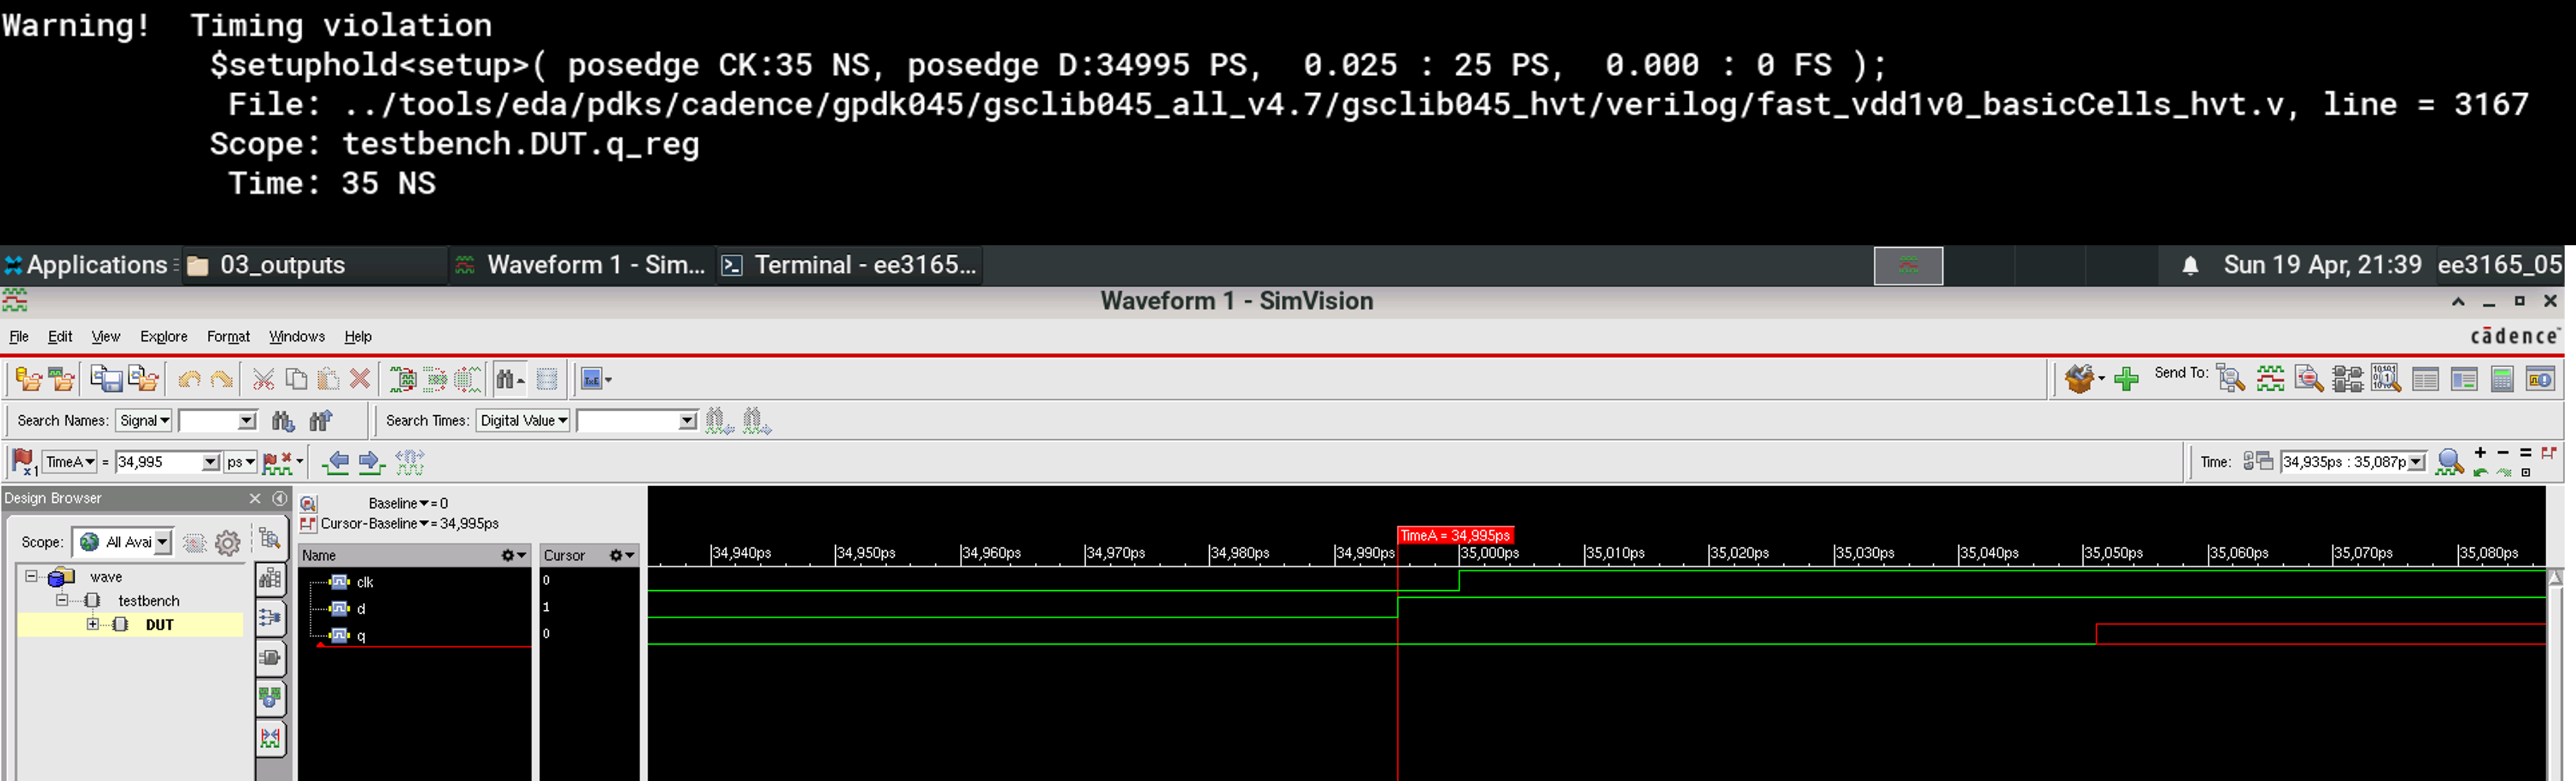
\includegraphics[width=\textwidth]{figures/dff_hvt_fast1v0_setup_posedge.png}
        \caption{D posedge: $\Delta t = 0.005$\,ns $<$ 0.025\,ns $\Rightarrow$ Q bị lỗi}
    \end{subfigure}
    \hfill
    \begin{subfigure}[b]{0.75\textwidth}
        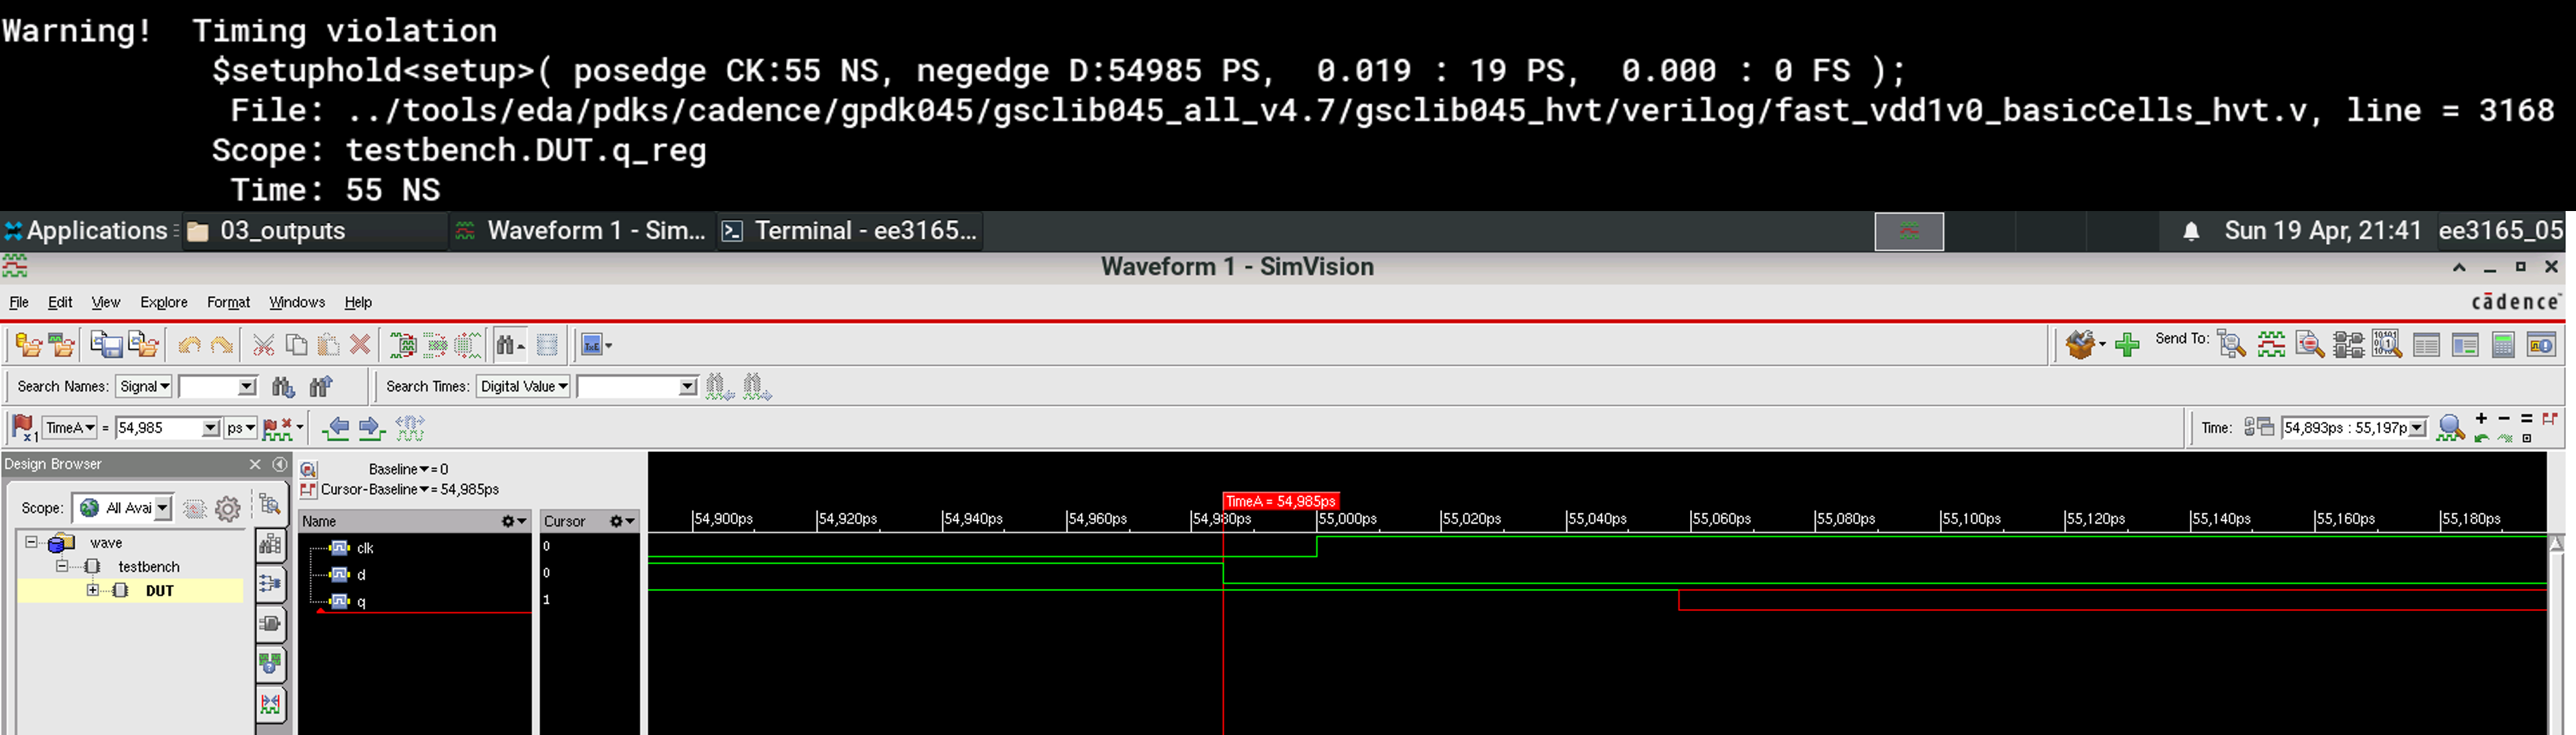
\includegraphics[width=\textwidth]{figures/dff_hvt_fast1v0_setup_negedge.png}
        \caption{D negedge: $\Delta t = 0.015$\,ns $<$ 0.019\,ns $\Rightarrow$ Q bị lỗi}
    \end{subfigure}
    \caption{Kiểm chứng vi phạm Setup Time của D-FF HVT tại VDD = 1.0\,V.}
    \label{fig:dff_hvt_fast1v0_setup}
\end{figure}

Tại corner \texttt{slow\_vdd1v0\_hvt}: Setup Time posedge D lên đến 0.177\,ns, đây là giá
trị lớn nhất trong 8 corners và là worst-case về ràng buộc thời gian. Hold Time
negedge D = 0.051\,ns $\neq 0$ -- đây là corner duy nhất trong nhóm HVT xuất hiện ràng
buộc Hold Time khác~0, yêu cầu kỹ sư thiết kế phải kiểm tra kỹ Hold Time violation.

\begin{figure}[H]
    \centering
    \begin{subfigure}[b]{0.75\textwidth}
        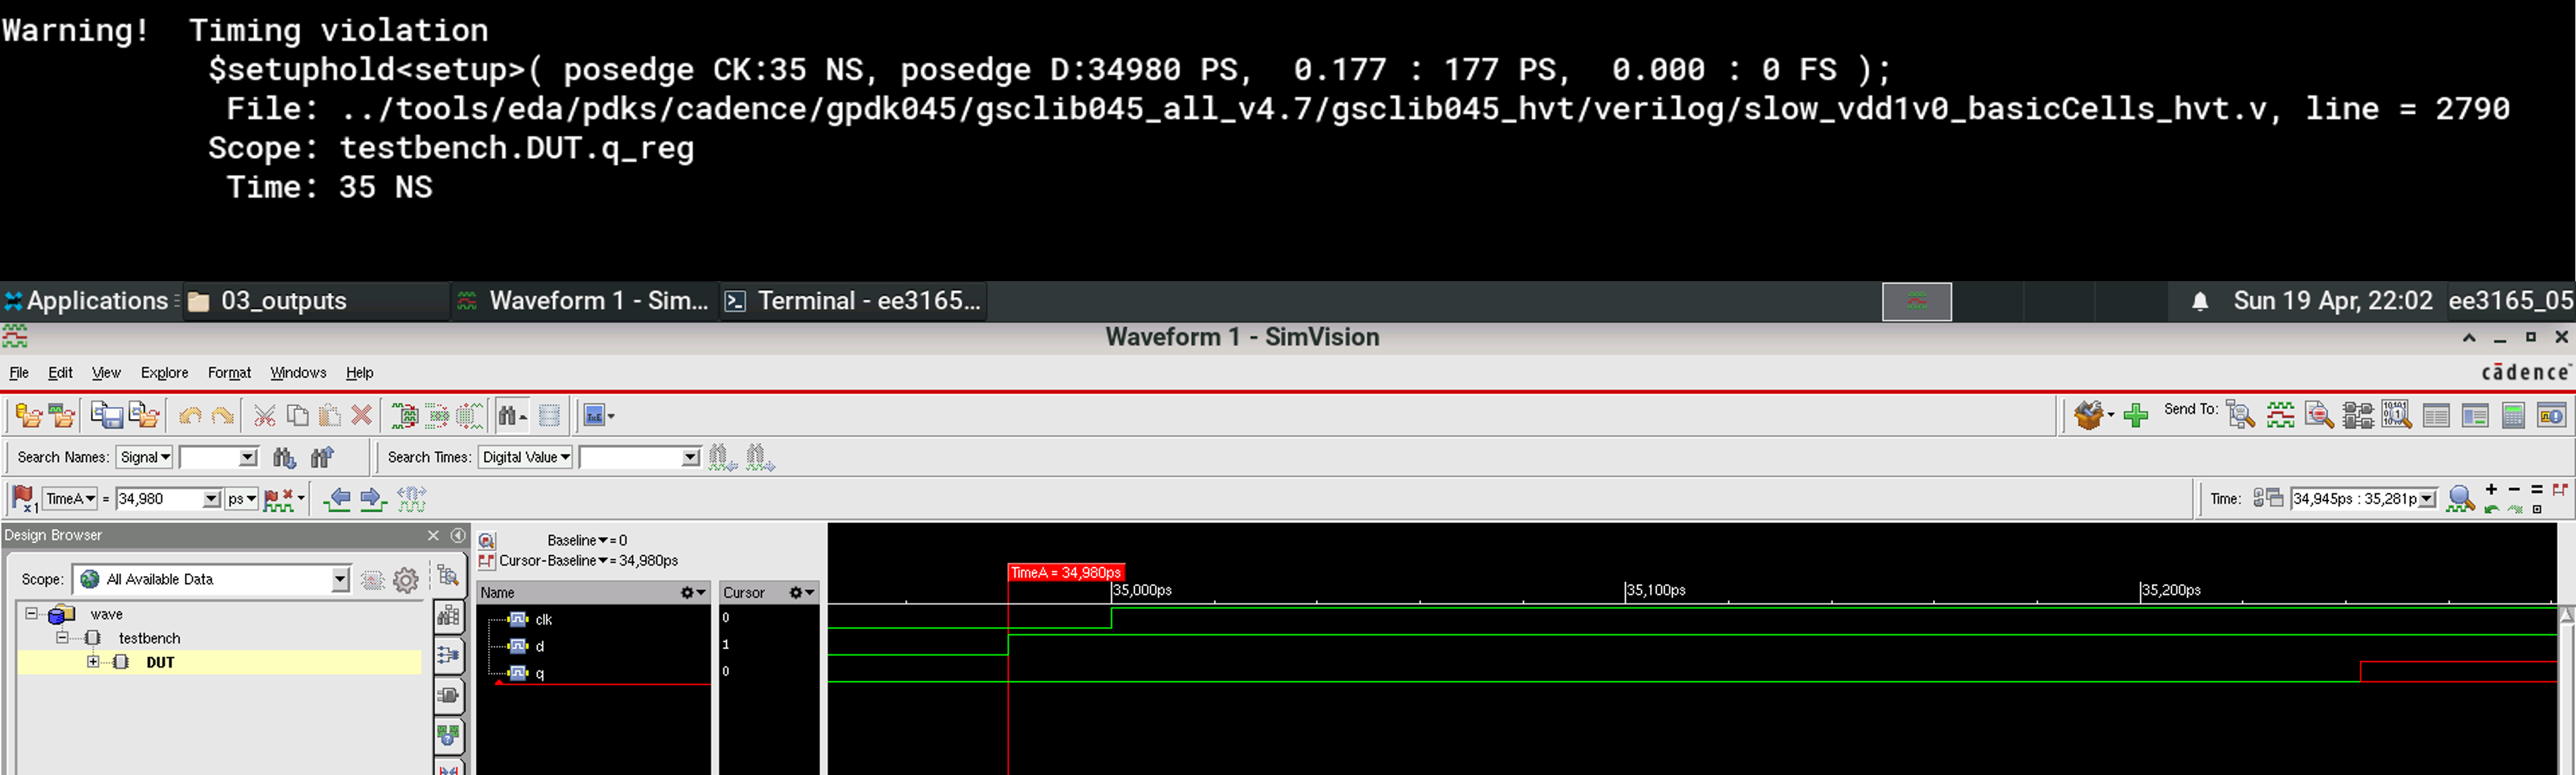
\includegraphics[width=\textwidth]{figures/dff_hvt_slow1v0_setup_posedge.png}
        \caption{D posedge: $\Delta t = 0.02$\,ns $<$ 0.177\,ns $\Rightarrow$ Q bị lỗi}
    \end{subfigure}
    \hfill 
    \begin{subfigure}[b]{0.75\textwidth}
        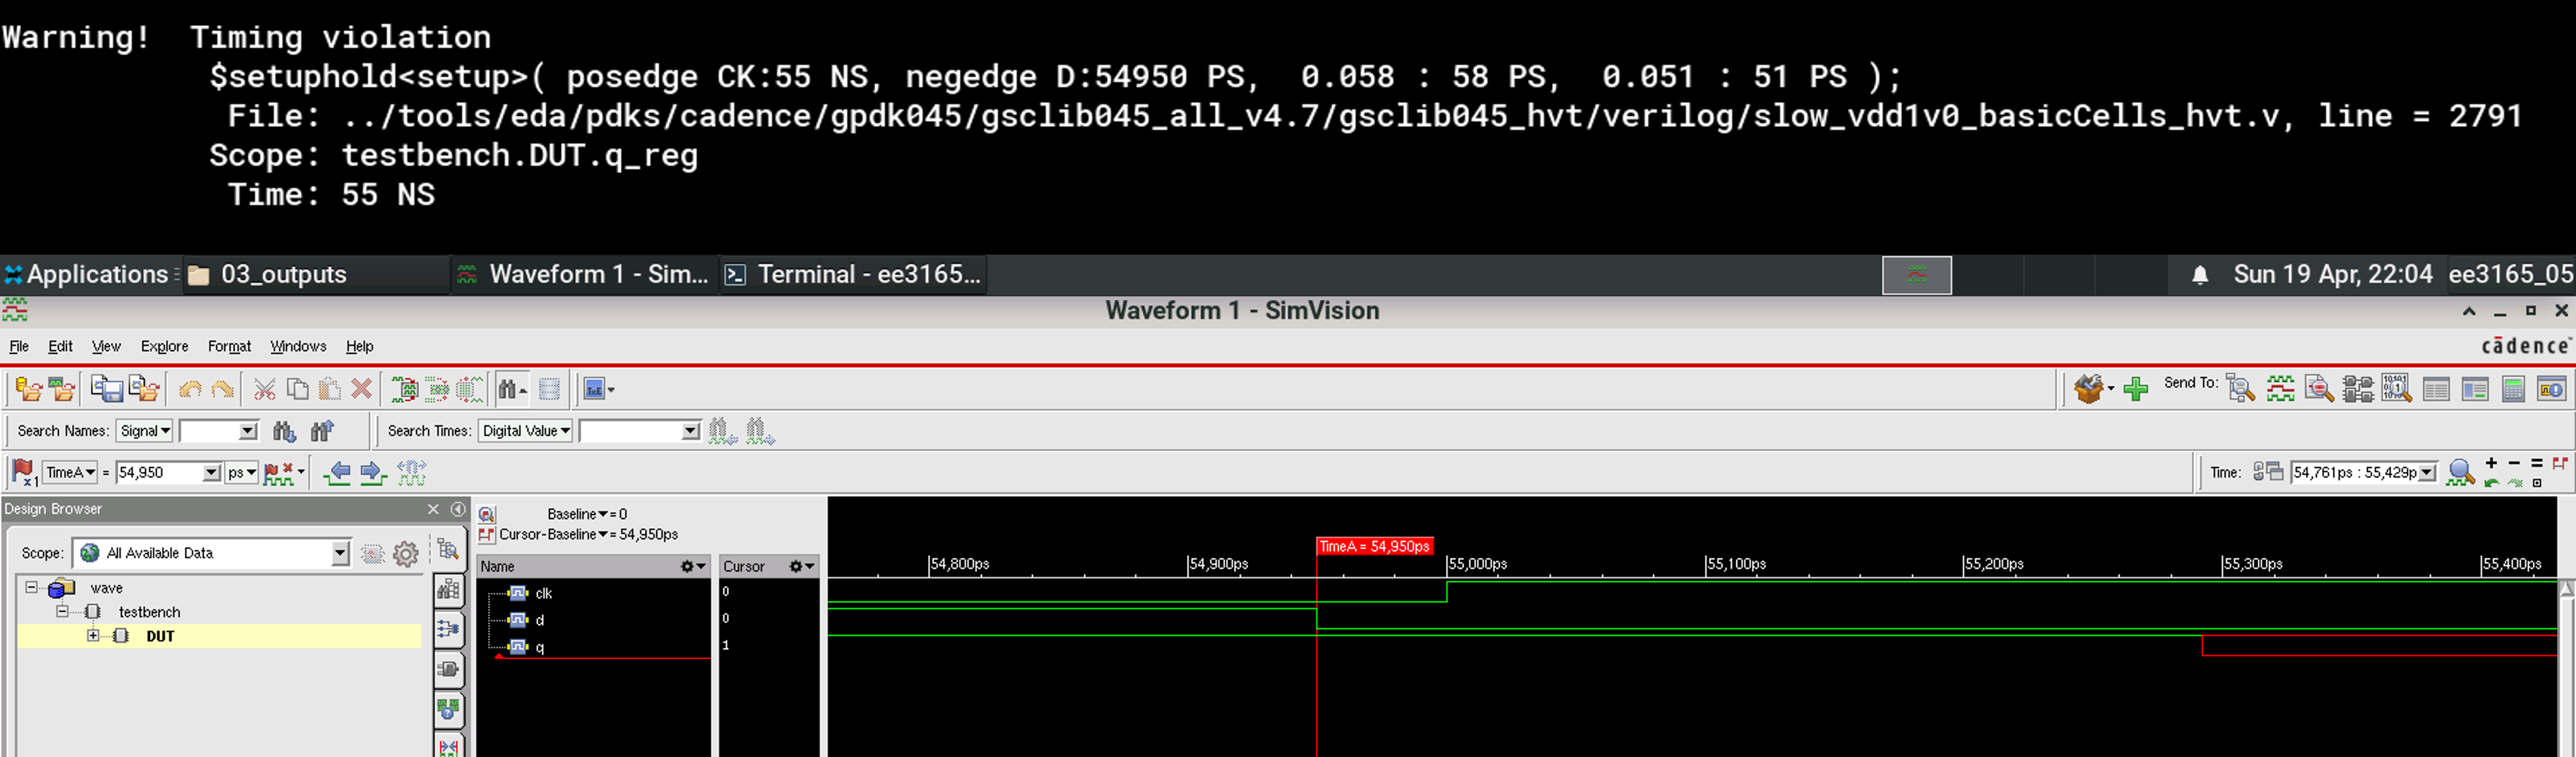
\includegraphics[width=\textwidth]{figures/dff_hvt_slow1v0_setup_negedge.png}
        \caption{D negedge: $\Delta t = 0.05$\,ns $<$ 0.058\,ns $\Rightarrow$ Q bị lỗi}
    \end{subfigure}
    \caption{Kiểm chứng vi phạm Setup Time của D-FF HVT tại VDD = 1.0\,V (Slow corner).}
    \label{fig:dff_hvt_slow1v0_setup}
\end{figure}

\paragraph{2. Kiểm chứng HVT tại VDD = 1.2\,V}

\begin{figure}[H]
    \centering
    \begin{subfigure}[b]{0.75\textwidth}
        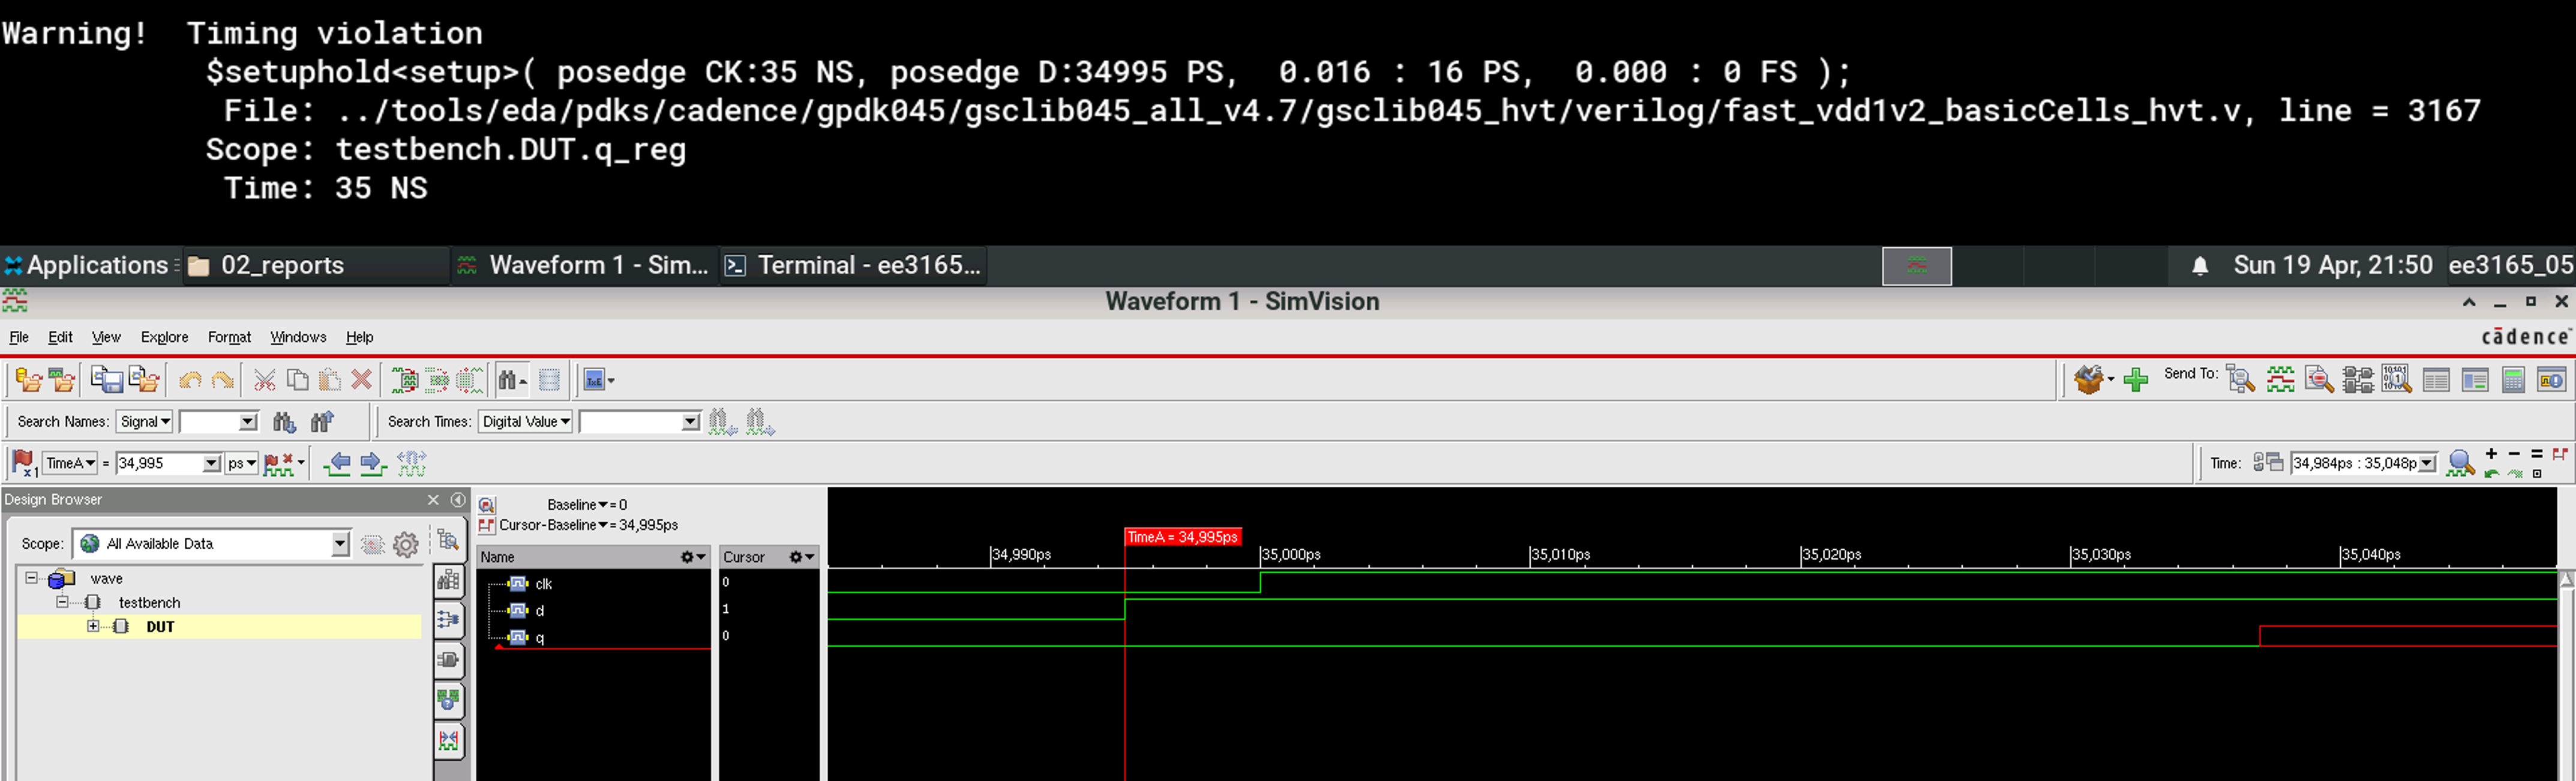
\includegraphics[width=\textwidth]{figures/dff_hvt_fast1v2_setup_posedge.png}
        \caption{D posedge: $\Delta t = 0.005$\,ns $<$ 0.016\,ns $\Rightarrow$ Q bị lỗi}
    \end{subfigure}
    \hfill
    \begin{subfigure}[b]{0.75\textwidth}
        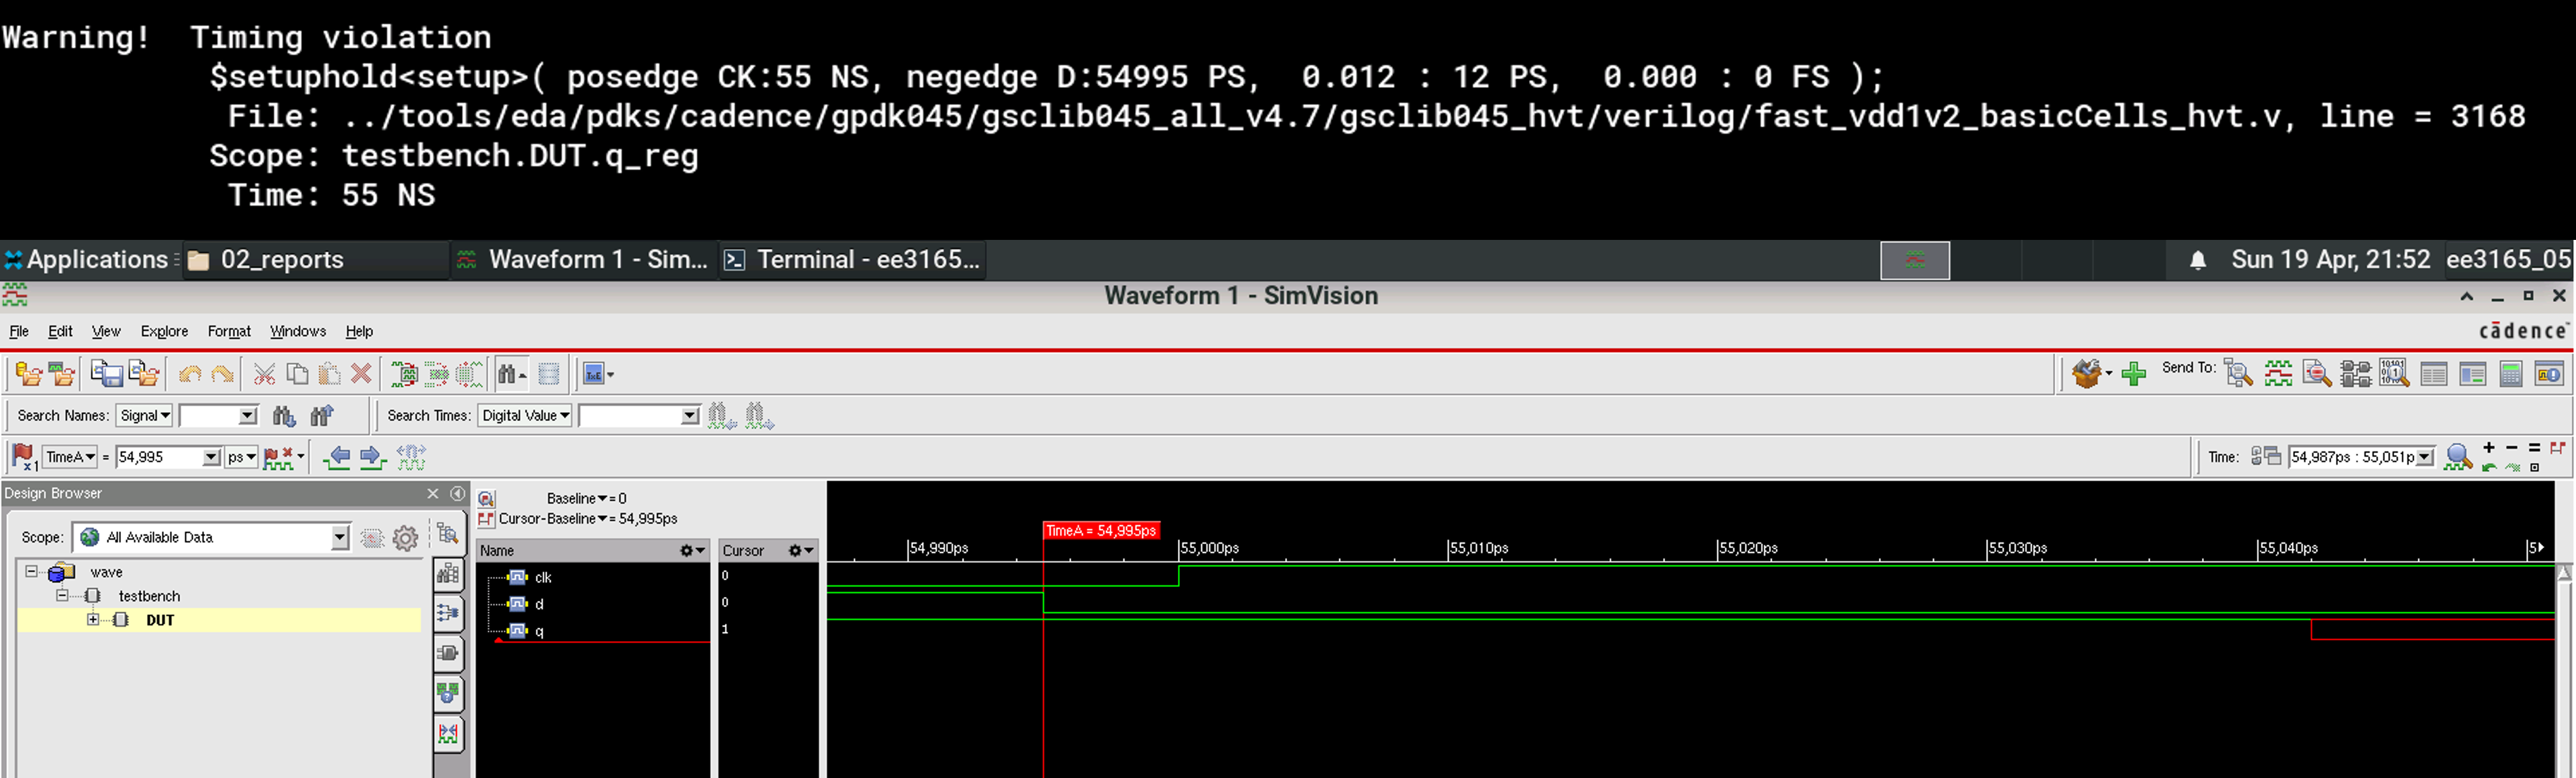
\includegraphics[width=\textwidth]{figures/dff_hvt_fast1v2_setup_negedge.png}
        \caption{D negedge: $\Delta t = 0.005$\,ns $<$ 0.012\,ns $\Rightarrow$ Q bị lỗi}
    \end{subfigure}
    \caption{Kiểm chứng vi phạm Setup Time của D-FF HVT tại VDD = 1.2\,V (Fast corner).}
    \label{fig:dff_hvt_fast1v2_setup}
\end{figure}

\begin{figure}[H]
    \centering
    \begin{subfigure}[b]{0.75\textwidth}
        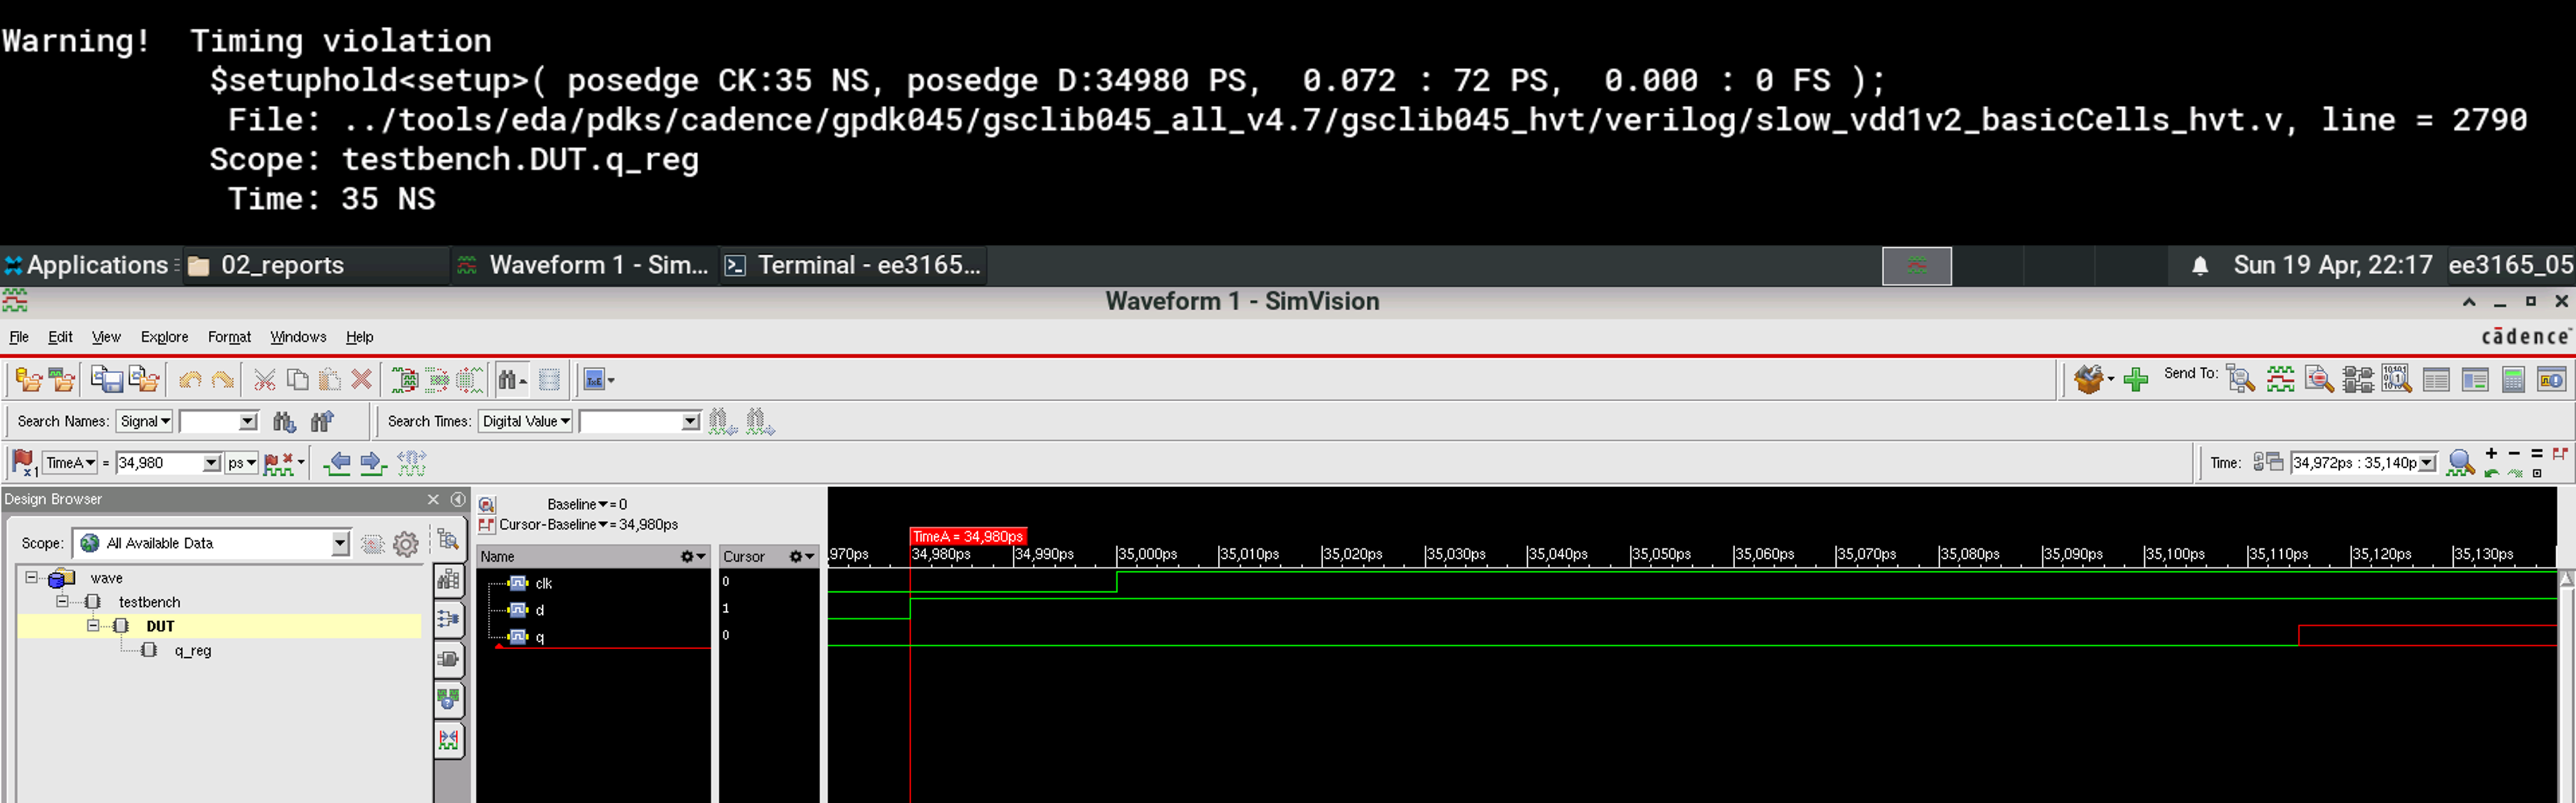
\includegraphics[width=\textwidth]{figures/dff_hvt_slow1v2_setup_posedge.png}
        \caption{D posedge: $\Delta t = 0.02$\,ns $<$ 0.072\,ns $\Rightarrow$ Q bị lỗi}
    \end{subfigure}
    \hfill
    \begin{subfigure}[b]{0.75\textwidth}
        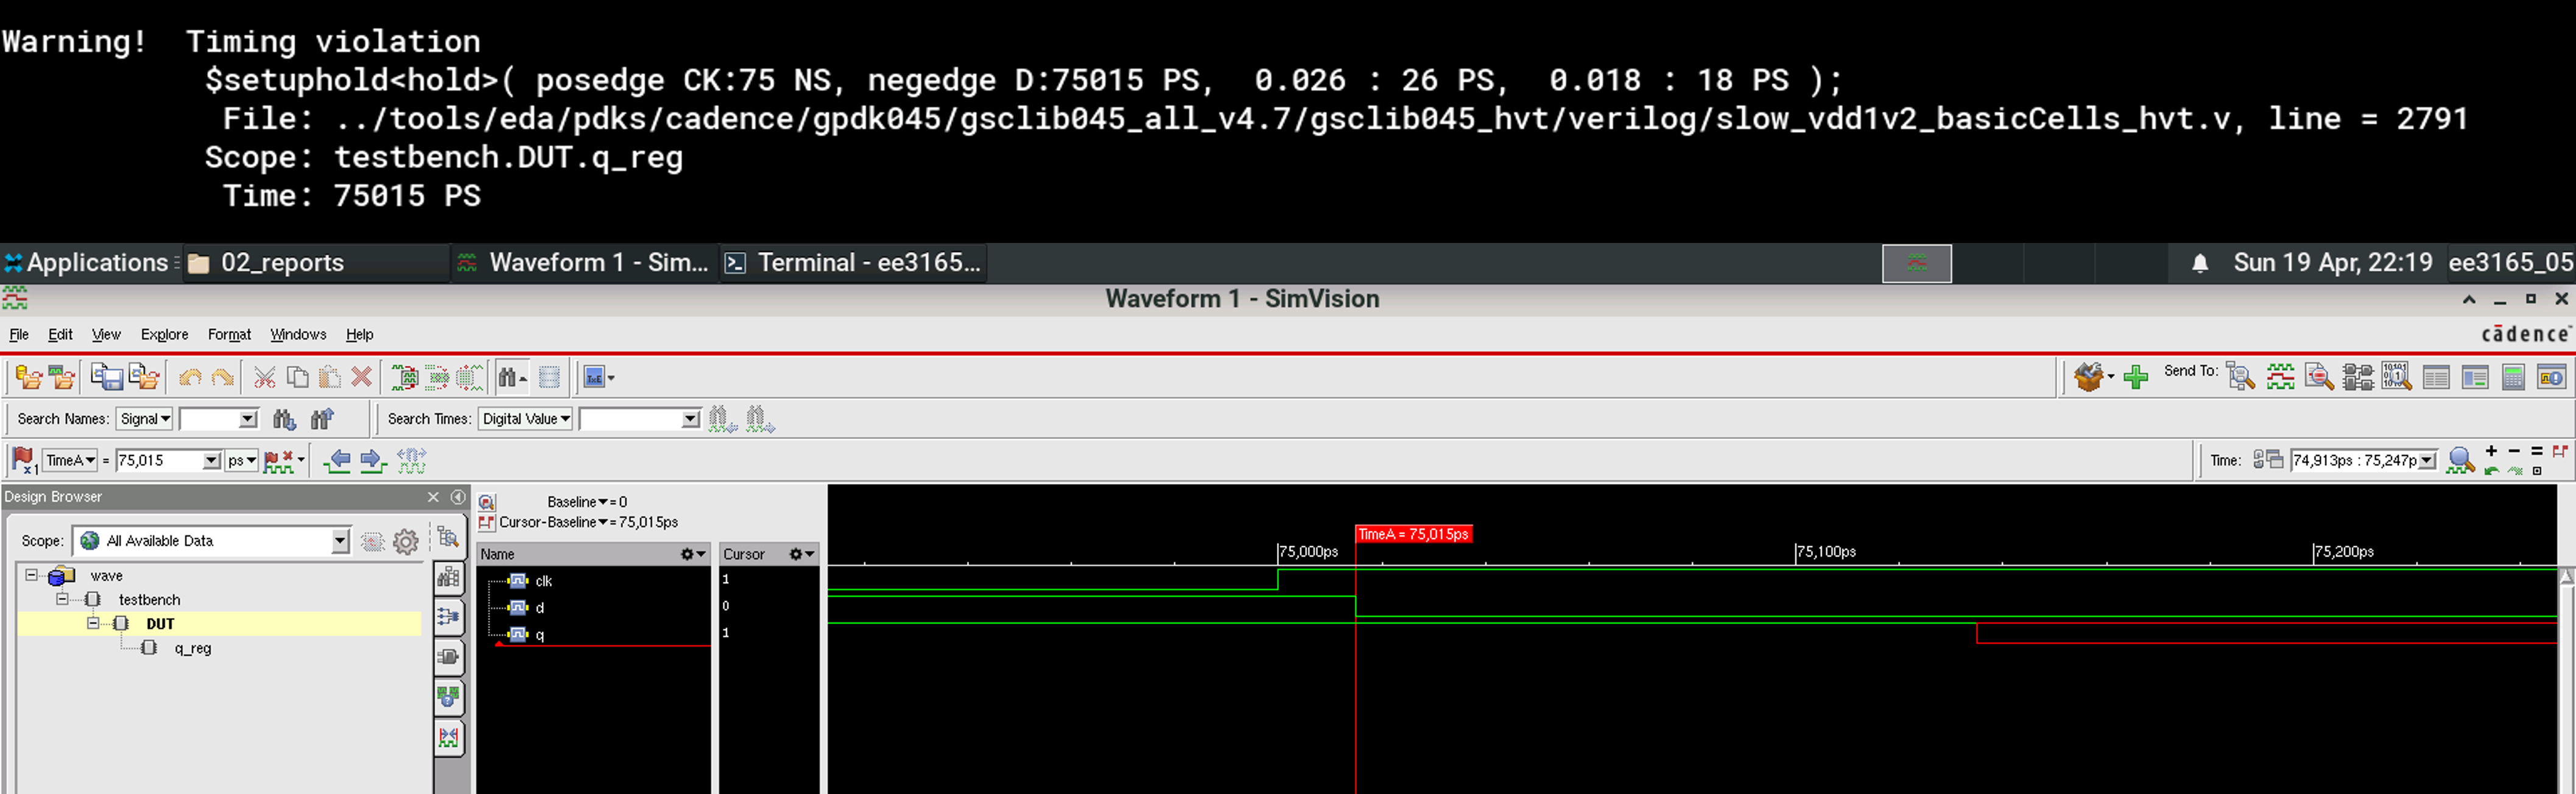
\includegraphics[width=\textwidth]{figures/dff_hvt_slow1v2_hold_negedge.png}
        \caption{D negedge Hold: $\Delta t = 0.015$\,ns $<$ 0.018\,ns $\Rightarrow$ Q bị lỗi}
    \end{subfigure}
    \caption{Kiểm chứng vi phạm Setup và Hold Time của D-FF HVT tại VDD = 1.2\,V (Slow corner).}
    \label{fig:dff_hvt_slow1v2}
\end{figure}

\subsubsection*{B. Thư viện Low Threshold Voltage (LVT)}

\paragraph{1. Kiểm chứng LVT tại VDD = 1.0\,V}

\begin{figure}[H]
    \centering
    \begin{subfigure}[b]{0.75\textwidth}
        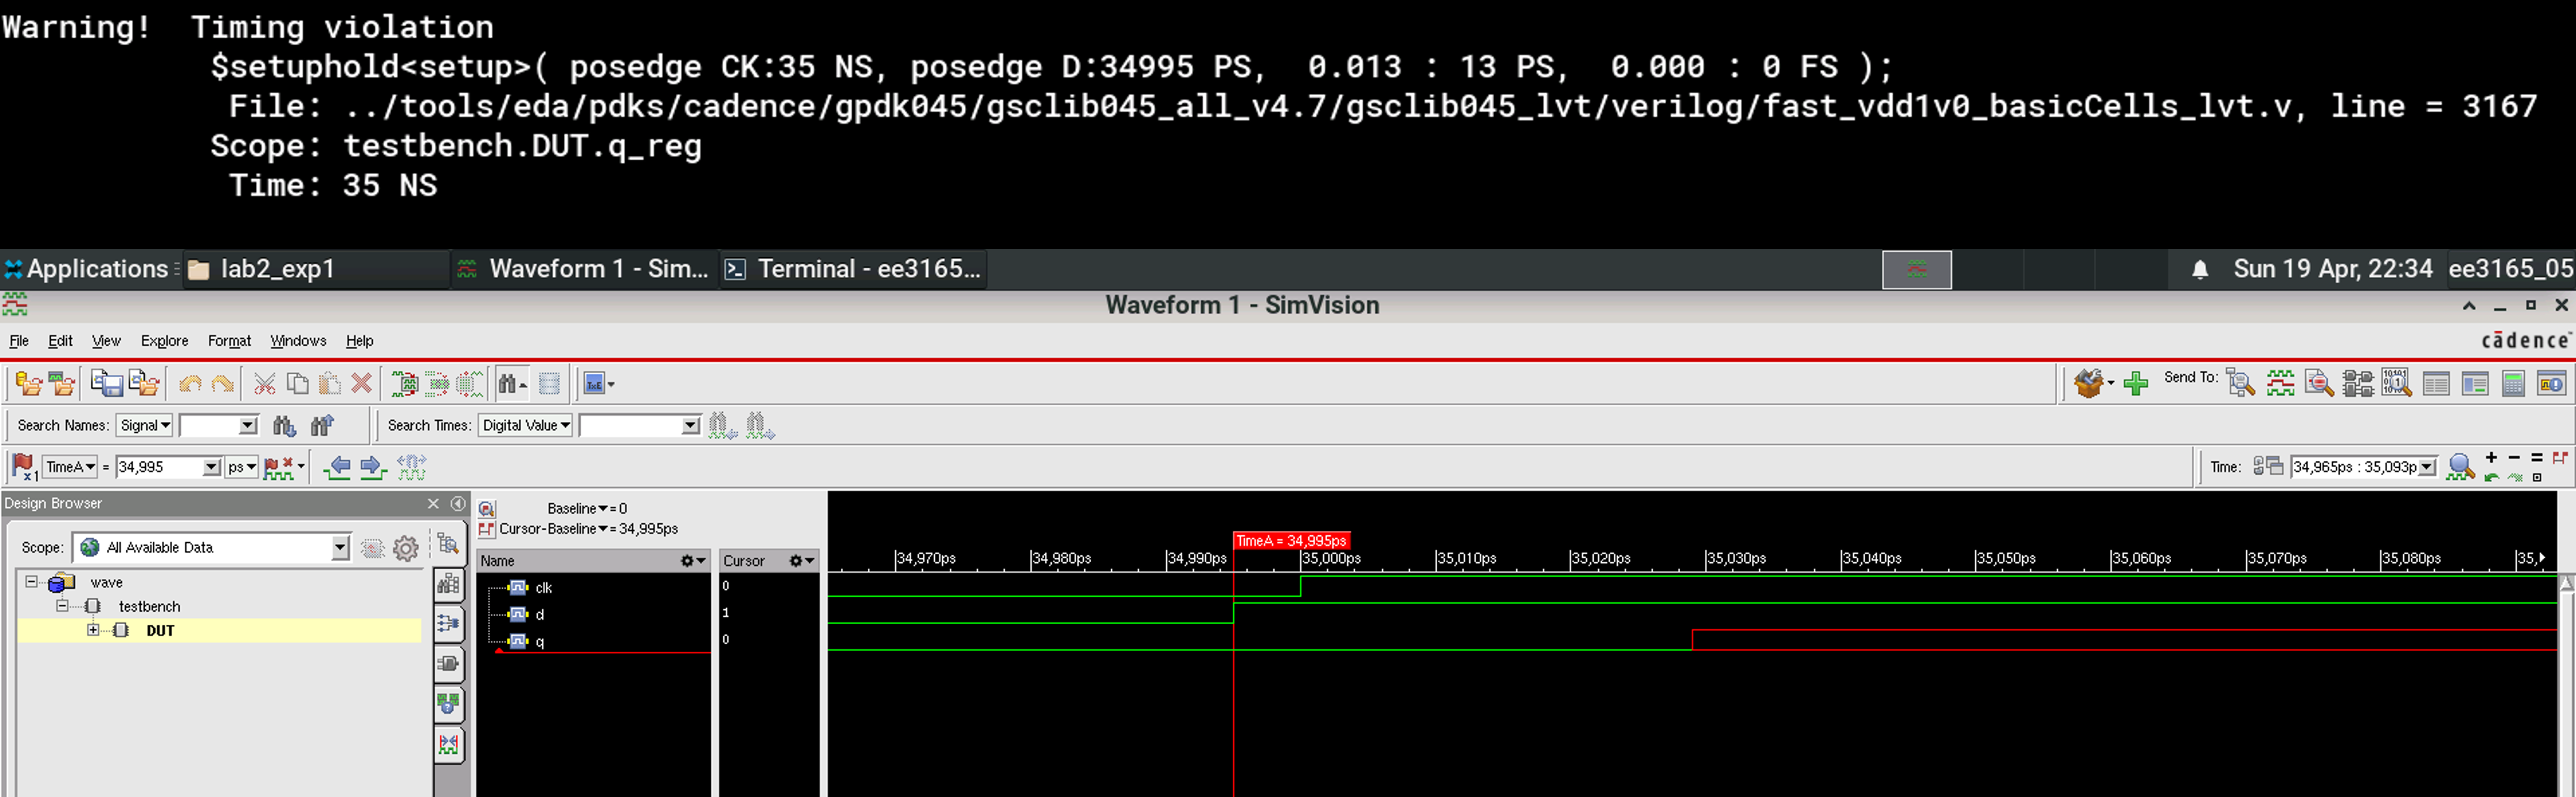
\includegraphics[width=\textwidth]{figures/dff_lvt_fast1v0_setup_posedge.png}
        \caption{D posedge: $\Delta t = 0.005$\,ns $<$ 0.013\,ns $\Rightarrow$ Q bị lỗi}
    \end{subfigure}
    \hfill
    \begin{subfigure}[b]{0.75\textwidth}
        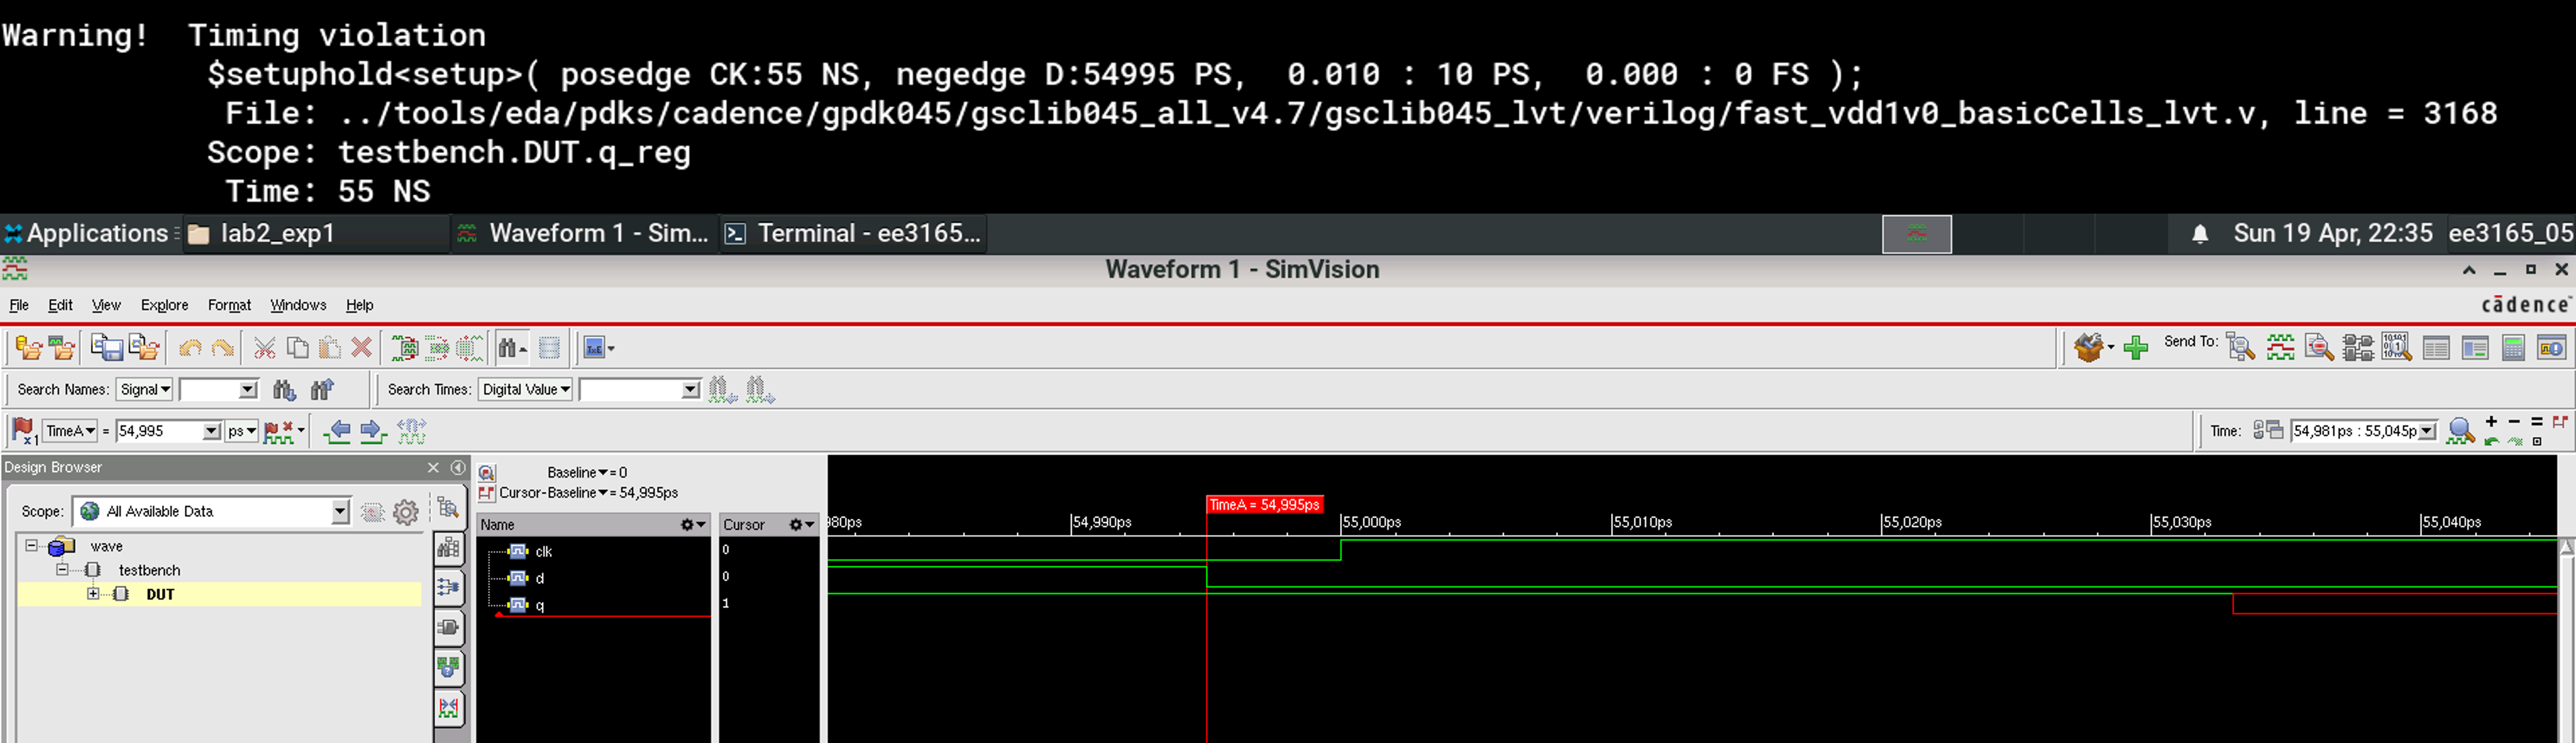
\includegraphics[width=\textwidth]{figures/dff_lvt_fast1v0_setup_negedge.png}
        \caption{D negedge: $\Delta t = 0.005$\,ns $<$ 0.010\,ns $\Rightarrow$ Q bị lỗi}
    \end{subfigure}
    \caption{Kiểm chứng vi phạm Setup Time của D-FF LVT tại VDD = 1.0\,V (Fast corner).}
    \label{fig:dff_lvt_fast1v0_setup}
\end{figure}

\begin{figure}[H]
    \centering
    \begin{subfigure}[b]{0.75\textwidth}
        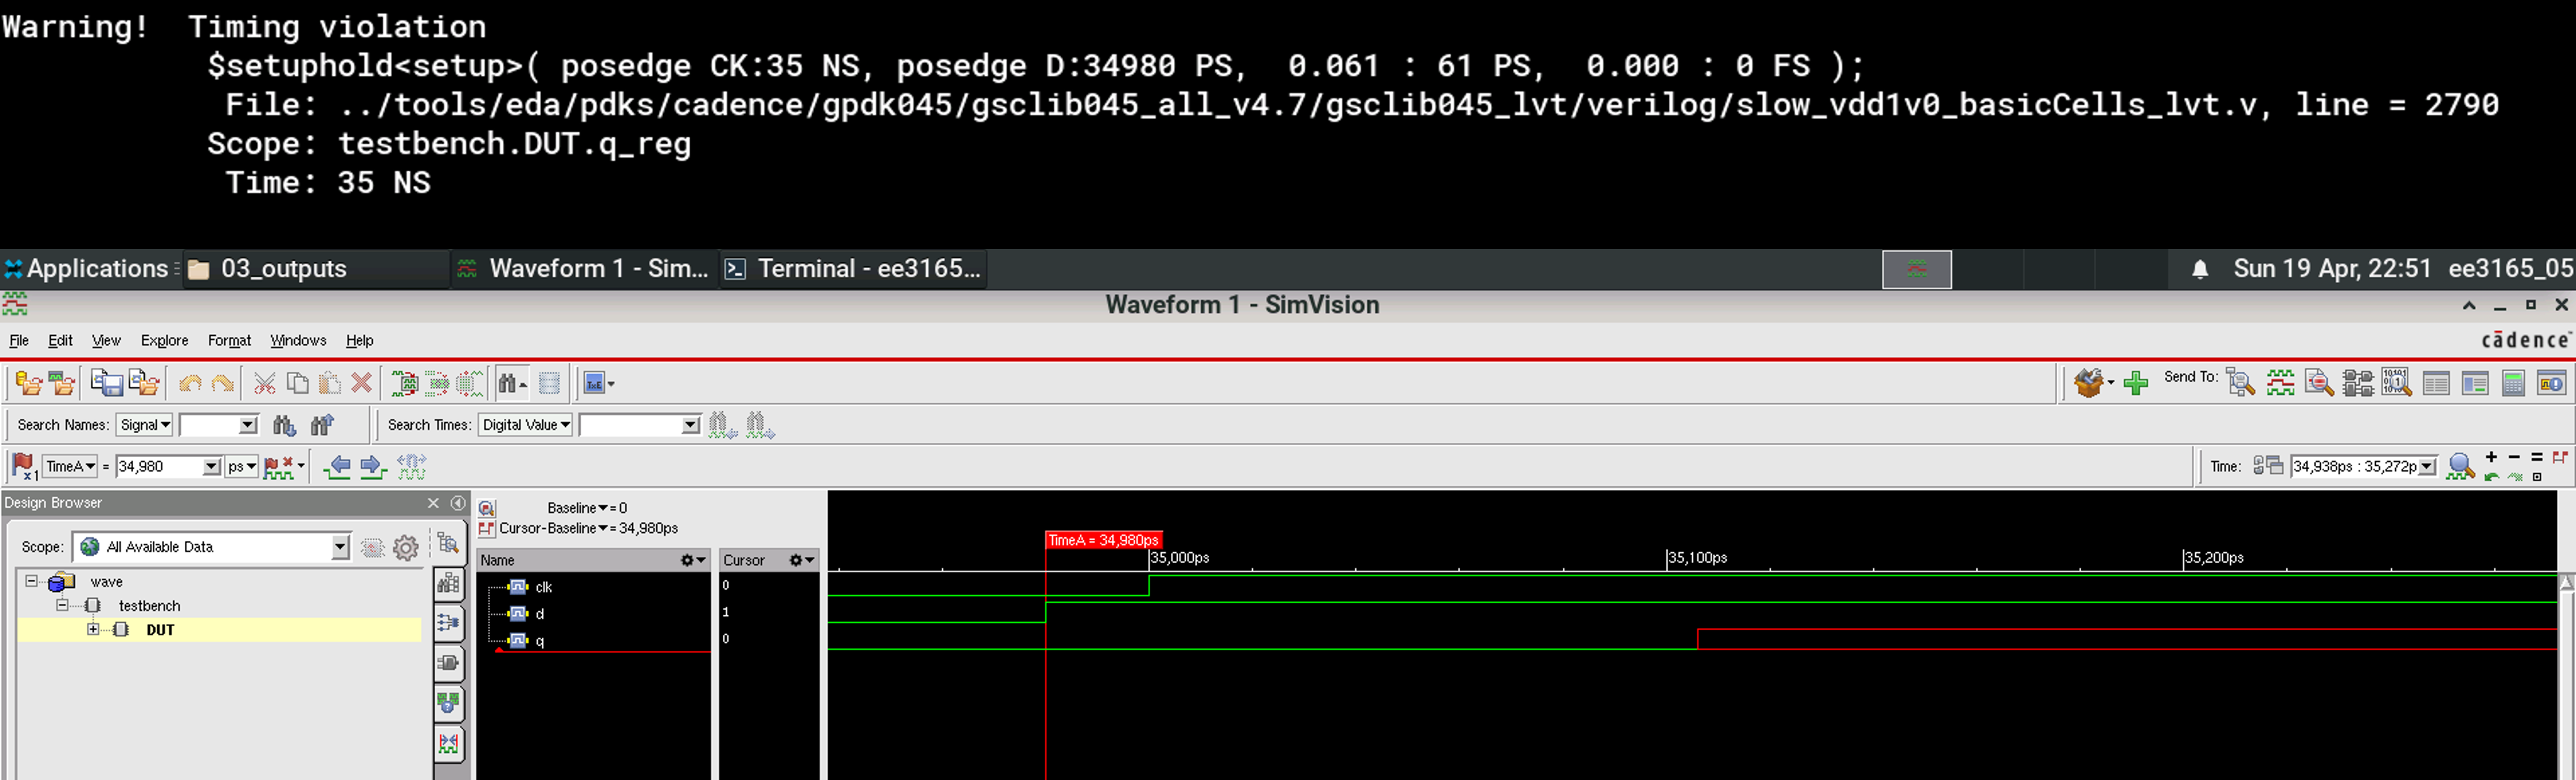
\includegraphics[width=\textwidth]{figures/dff_lvt_slow1v0_setup_posedge.png}
        \caption{D posedge: $\Delta t = 0.02$\,ns $<$ 0.061\,ns $\Rightarrow$ Q bị lỗi}
    \end{subfigure}

    \begin{subfigure}[b]{0.75\textwidth}
        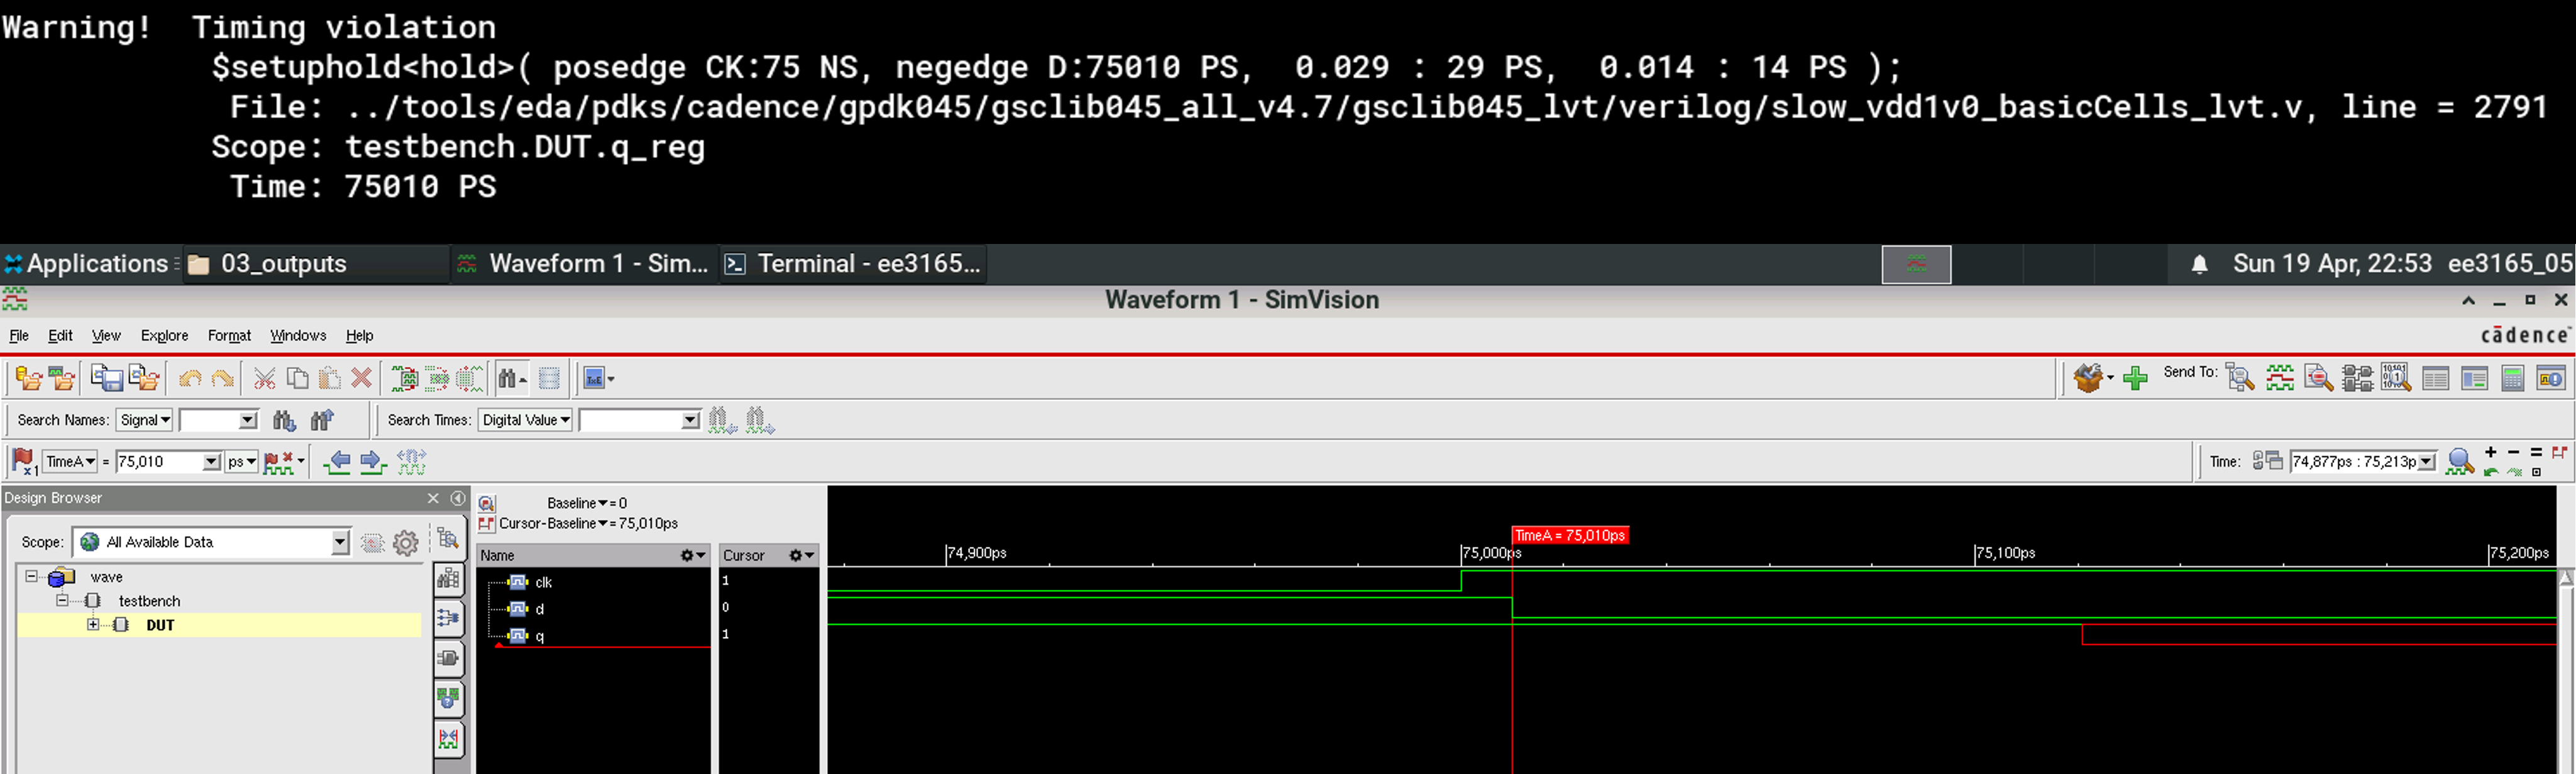
\includegraphics[width=\textwidth]{figures/dff_lvt_slow1v0_hold_negedge.png}
        \caption{D negedge Hold: $\Delta t = 0.01$\,ns $<$ 0.014\,ns $\Rightarrow$ Q bị lỗi}
    \end{subfigure}
    \caption{Kiểm chứng vi phạm Setup và Hold Time của D-FF LVT tại VDD = 1.0\,V (Slow corner).}
    \label{fig:dff_lvt_slow1v0}
\end{figure}

\paragraph{2. Kiểm chứng LVT tại VDD = 1.2\,V}

\begin{figure}[H]
    \centering
    \begin{subfigure}[b]{0.8\textwidth}
        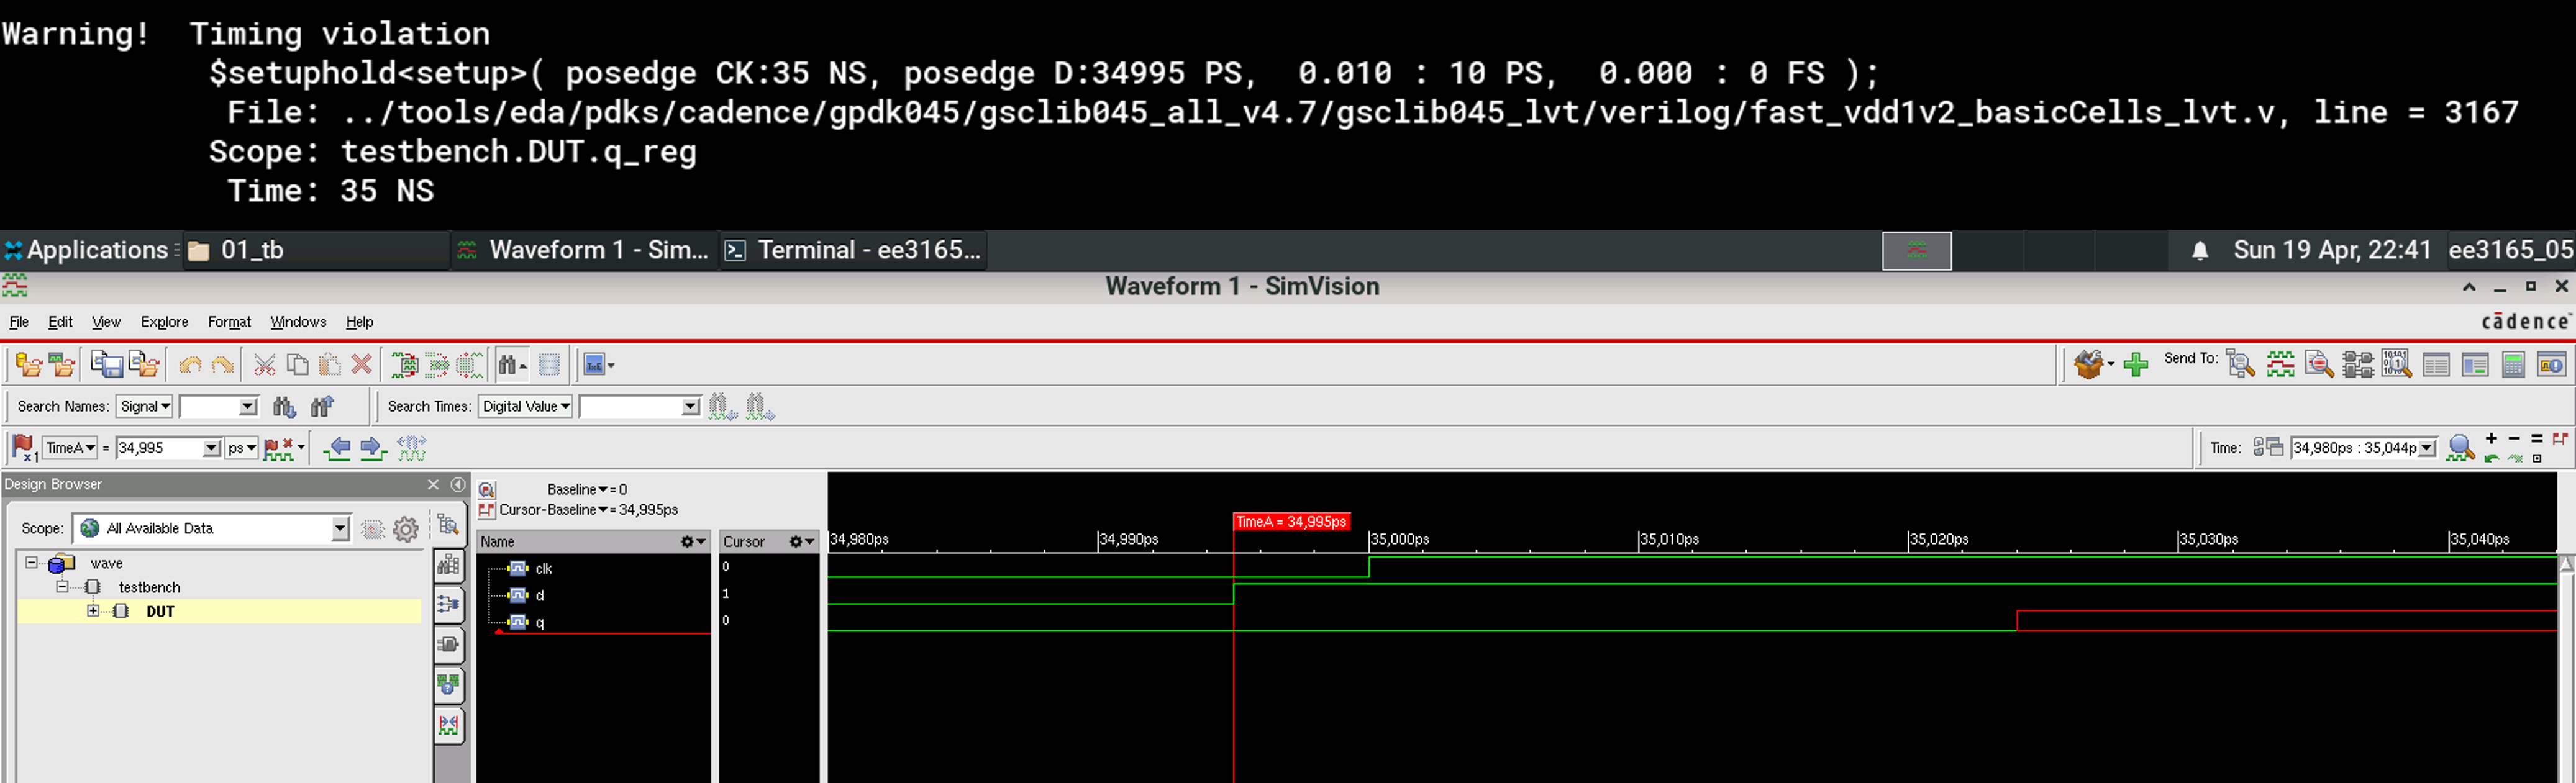
\includegraphics[width=\textwidth]{figures/dff_lvt_fast1v2_setup_posedge.png}
        \caption{D posedge: $\Delta t = 0.005$\,ns $<$ 0.010\,ns $\Rightarrow$ Q bị lỗi}
    \end{subfigure}
    \hfill
    \begin{subfigure}[b]{0.8\textwidth}
        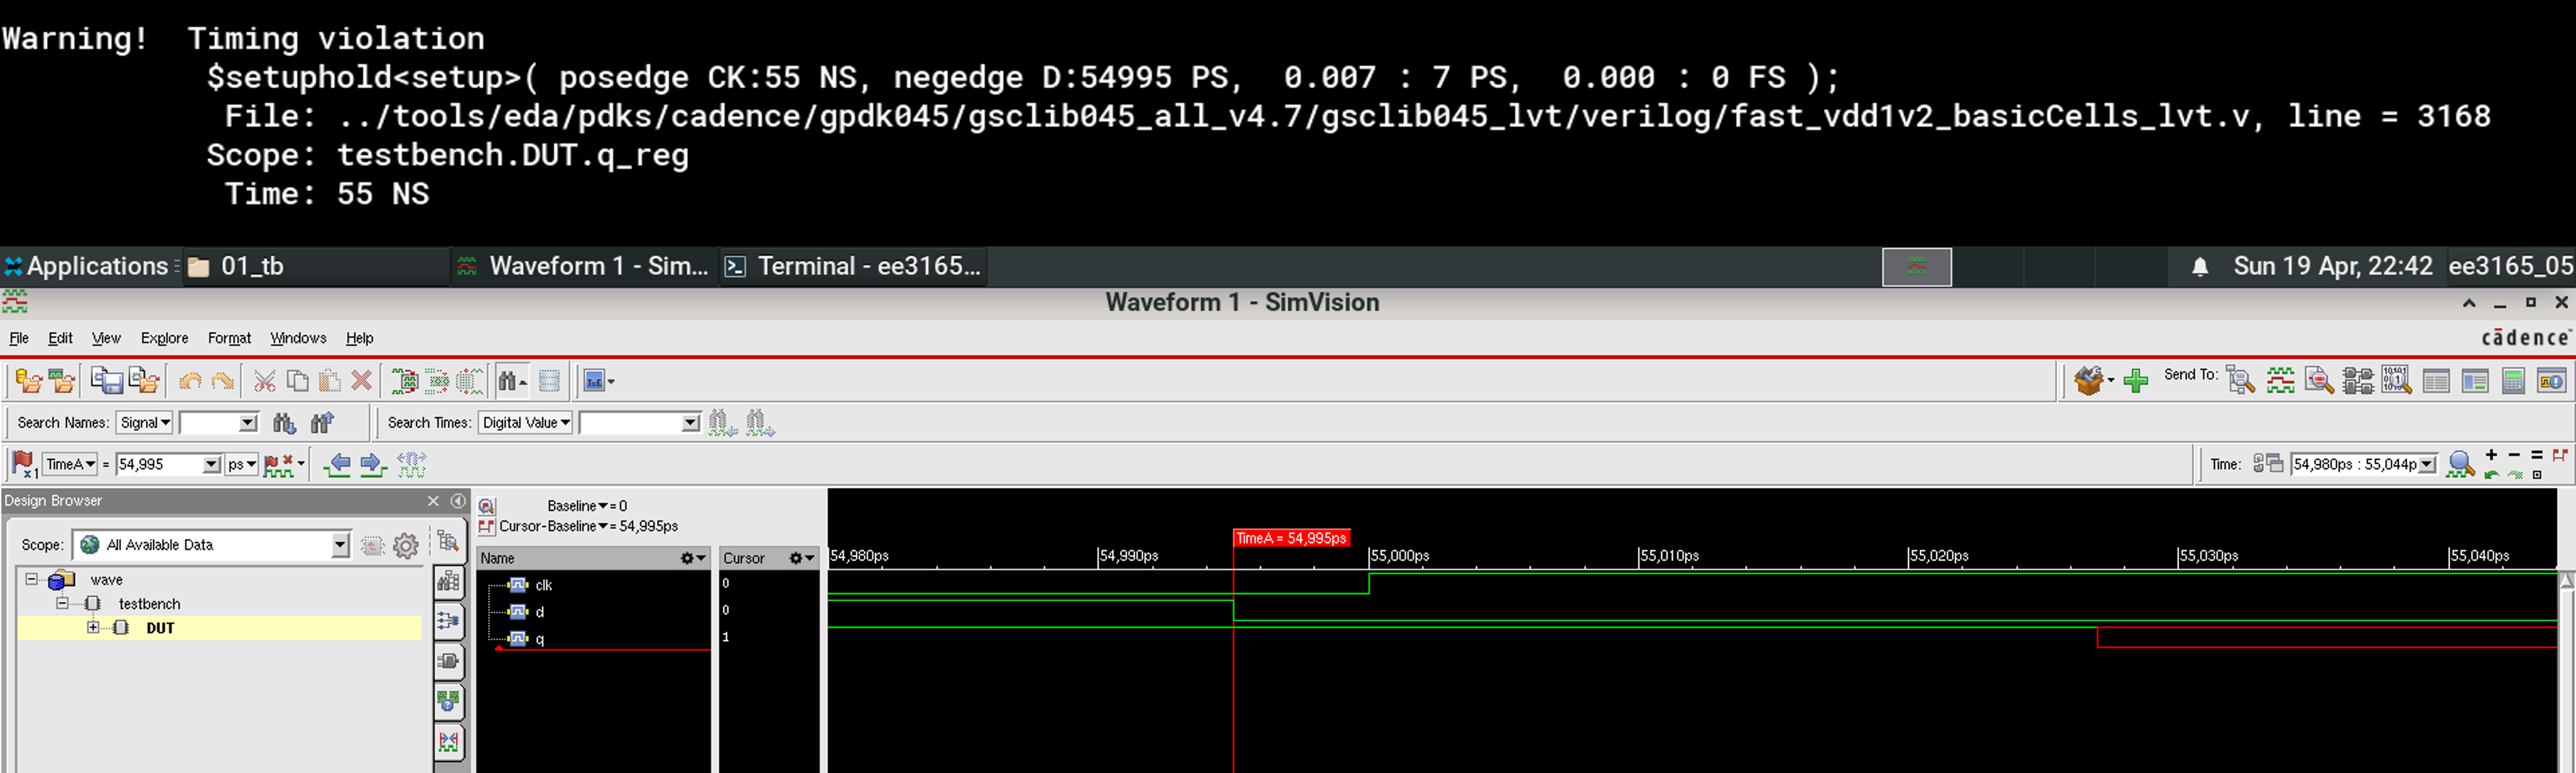
\includegraphics[width=\textwidth]{figures/dff_lvt_fast1v2_setup_negedge.png}
        \caption{D negedge: $\Delta t = 0.005$\,ns $<$ 0.007\,ns $\Rightarrow$ Q bị lỗi}
    \end{subfigure}
    \caption{Kiểm chứng vi phạm Setup Time của D-FF LVT tại VDD = 1.2\,V (Fast corner).}
    \label{fig:dff_lvt_fast1v2_setup}
\end{figure}

\begin{figure}[H]
    \centering
    \begin{subfigure}[b]{0.8\textwidth}
        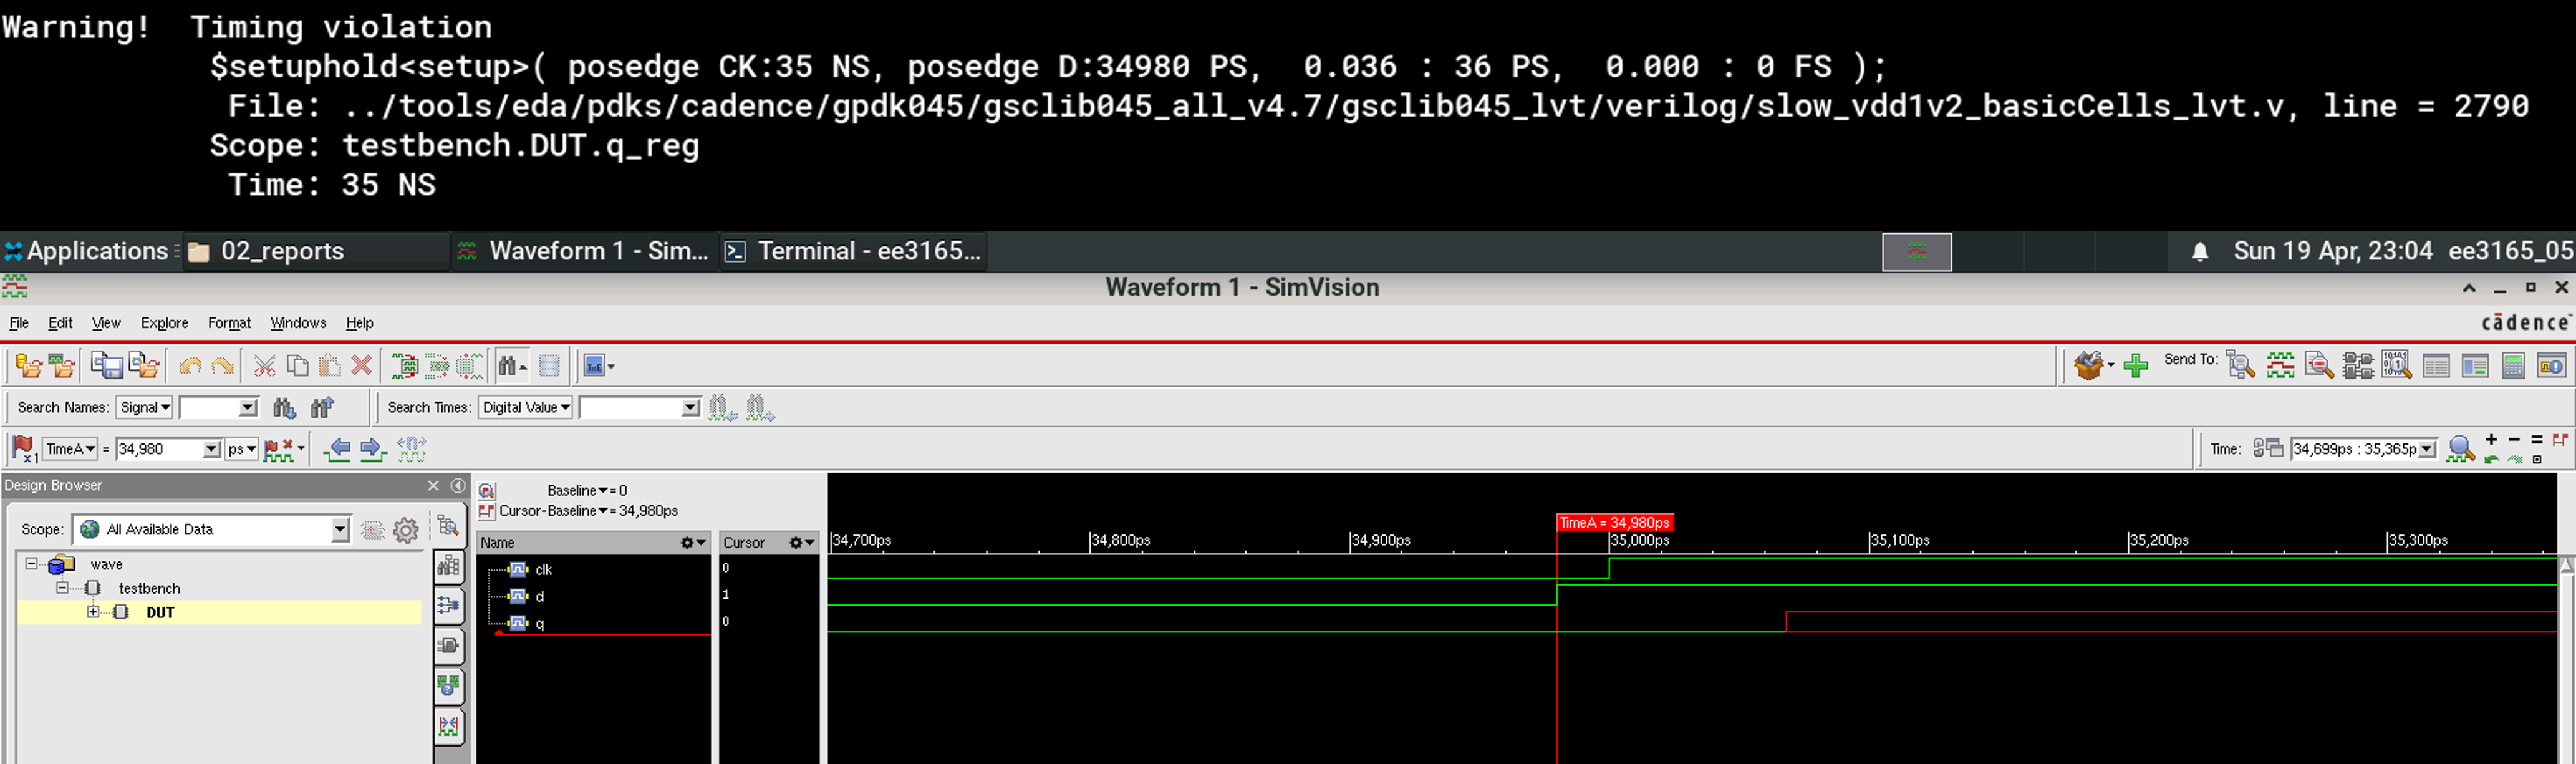
\includegraphics[width=\textwidth]{figures/dff_lvt_slow1v2_setup_posedge.png}
        \caption{D posedge: $\Delta t = 0.02$\,ns $<$ 0.036\,ns $\Rightarrow$ Q bị lỗi}
    \end{subfigure}
    \hfill
    \begin{subfigure}[b]{0.8\textwidth}
        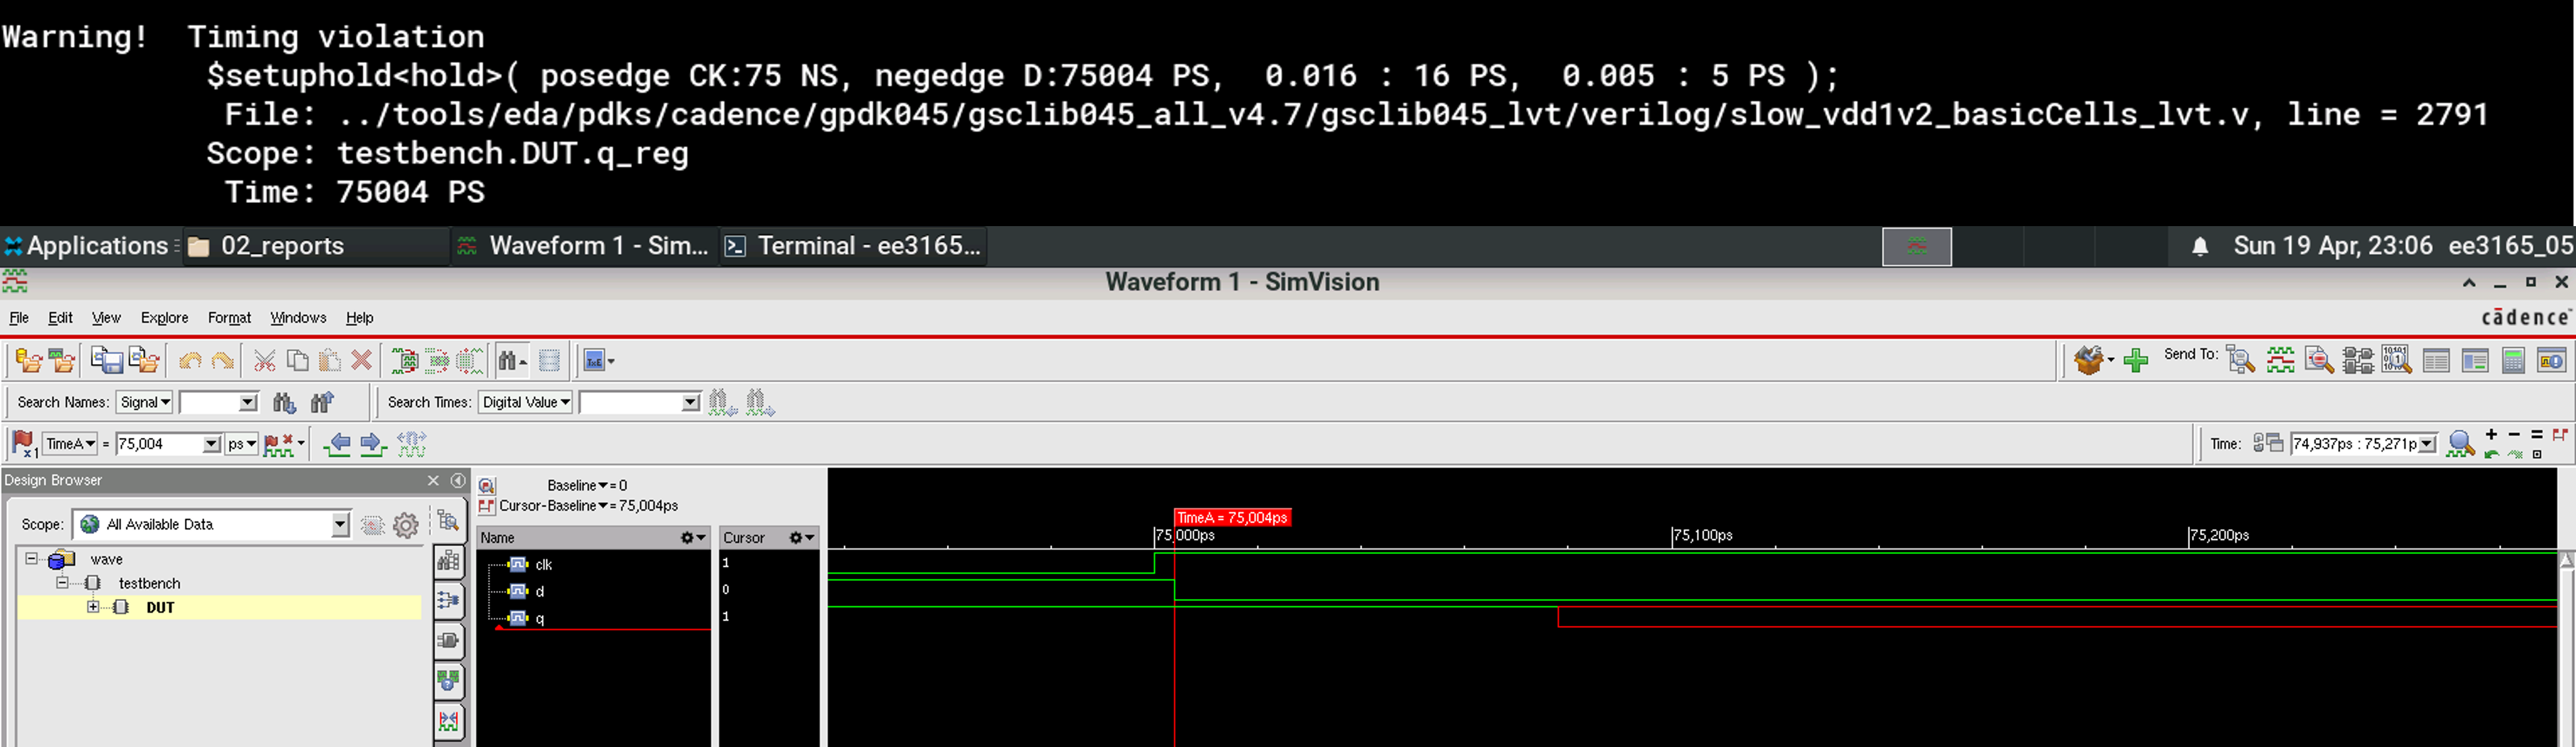
\includegraphics[width=\textwidth]{figures/dff_lvt_slow1v2_hold_negedge.png}
        \caption{D negedge Hold: $\Delta t = 0.004$\,ns $<$ 0.005\,ns $\Rightarrow$ Q bị lỗi}
    \end{subfigure}
    \caption{Kiểm chứng vi phạm Setup và Hold Time của D-FF LVT tại VDD = 1.2\,V (Slow corner).}
    \label{fig:dff_lvt_slow1v2}
\end{figure}

\subsubsection*{C. Kết luận về Setup và Hold Time}

Qua việc kiểm chứng vi phạm timing trên cả 8 corners, nhóm rút ra các nhận xét quan
trọng sau:

\begin{itemize}
    \item \textbf{Setup Time tăng mạnh ở góc Slow--1.0\,V--HVT:} Corner
    \texttt{slow\_vdd1v0\_hvt} có Setup Time posedge D lên đến 0.177\,ns -- gấp 7 lần so
    với \texttt{fast\_vdd1v2\_lvt} (0.024\,ns). Đây chính là \emph{worst-case timing path}
    mà kỹ sư phải ưu tiên đảm bảo khi sign-off.
    \item \textbf{Hold Time xuất hiện ở các góc Slow:} Điều đáng lưu ý là Hold Time $\neq 0$
    chỉ xuất hiện ở hai corners \texttt{slow\_vdd1v0} (cả HVT và LVT), \texttt{slow\_vdd1v2}
    (cả HVT và LVT). Ở các góc Fast, Hold Time bằng 0 -- tức là không có ràng buộc giữ dữ liệu.
    Điều này có nghĩa kỹ sư cần đặc biệt chú ý đến Hold Time violation khi mạch vận hành ở
    điều kiện Slow corner.
    \item \textbf{Tầm quan trọng của SDF annotation:} Chỉ khi chạy Gate-level simulation với
    file SDF được chú thích đầy đủ, mô phỏng mới phản ánh đúng hành vi timing thực tế của
    mạch. Mô phỏng RTL thuần túy không thể phát hiện các vi phạm Setup/Hold Time này.
\end{itemize}

% =========================================================

\section{Kết luận tổng kết}
Thông qua Lab 2: Synthesis và Standard Cell, nhóm đã đạt được những kết quả và hiểu biết sâu sắc về quy trình thiết kế vi mạch mức vật lý:
\begin{itemize}
    \item \textbf{Nắm vững luồng thiết kế:} Thành thạo việc viết mã RTL bằng SystemVerilog, viết Testbench kiểm chứng chức năng và sử dụng công cụ Genus để tổng hợp (Synthesis) ra sơ đồ mức cổng (Gate-level).
    \item \textbf{Phân tích đặc tính PVT:} Hiểu rõ bản chất vật lý của sự đánh đổi PPA (Power - Performance - Area). Nhận thức được nguyên nhân gây ra sự chênh lệch độ trễ do kiến trúc mạng Pull-up/Pull-down (như ở NAND và NOR), cũng như điểm nghẽn trên các đường dẫn tới hạn (như ngõ Cout của Full Adder).
    \item \textbf{Hiểu rành mạch về Timing Constraints:} Nắm vững cách các góc quy trình (FF, SS) tác động đến Setup Time và Hold Time của D-Flip Flop. Góc Slow thường là worst-case cho Setup Time, trong khi góc Fast quyết định các vi phạm về Hold Time.
    \item \textbf{Tối ưu hóa thiết kế (Multi-Vth):} Nắm được chiến lược phân bổ Standard Cell trong thực tế: Ưu tiên sử dụng cell HVT để tiết kiệm năng lượng rò rỉ và chỉ chèn cell LVT tại các đường truyền tới hạn để đảm bảo tần số hoạt động của chip.
\end{itemize}

\end{document}